
%%%%%%%%%%%%%%%%%%%%%%%%%%%%%  PREAMBLE  %%%%%%%%%%%%%%%%%%%%%%%%%%%%%

\documentclass[10pt,a4paper,openany]{book}

\usepackage{preamble}


%%%%%%%%%%%%%%%%%%%%%%%%%%%%%  DOCUMENT  %%%%%%%%%%%%%%%%%%%%%%%%%%%%%


% Boldface proof name
% \let\oldproofname=\proofname
% \renewcommand{\proofname}{\rm\bf{\oldproofname}}

% PORTADA/PREFACIO/ÍNDICE --------------------------------------------

\begin{document}
\frontmatter
\pagenumbering{roman}

% Portada
\begin{titlepage}
\newgeometry{top=4cm, bottom=3.5cm, left=3cm, right=3cm}
%
\centering
%
    {\includegraphics[width=0.2\textwidth]{Figures/LogoUsal.pdf}\par}
%
\vspace{.5cm}
% 
    {\bfseries\Large Universidad de Salamanca \par}
    \vspace{.3cm}
    {\scshape\large Facultad de Matem\'aticas \par}
%
\vspace{4cm}
%
    {\scshape\Huge Topolog\'ia \par}
    \vspace{.5cm}
    {\itshape\LARGE \thetitle \par}
%
    \vfill
%
     {\large \theauthor  \\
    Clases impartidas por Esteban G\'omez \par}
    \vspace{1cm}
    {\Large \thedate \par}
%
\restoregeometry
\end{titlepage}

 \tableofcontents

% Prefacio
%\include{Chapters/preface}
\cleardoublepage

% Índice
\let\cleardoublepage\clearpage %quita la página en blanco

% CUERPO -------------------------------------------------------------
\mainmatter
\pagenumbering{arabic}
\fancychapterstyle

\setcounter{chapter}{-1} \justifying
\chapter{Conceptos sobre teor\'ia de conjuntos}
\section{Conjuntos y pertenencia}

Sea $X$ un conjunto:
\begin{itemize}
    \item Si $x$ es un elemento de $X$, escribimos $x \in X$.
    \item Si consideramos el subconjunto unitario formado por $x$, escribimos $\{x\} \subseteq X$.
\end{itemize}

\begin{obs}
Los símbolos $\subset$ y $\subseteq$ se suelen emplear indistintamente en este contexto, pero es fundamental distinguir que:
$$
    x \in X \quad\text{no es lo mismo que}\quad \{x\} \subseteq X \text{}.
$$
\end{obs}

\paragraph{Partes de un conjunto:}
Dado un conjunto $X$, el \textbf{conjunto de las partes} de $X$, denotado por $\mathcal{P}(X)$, es la familia de todos los subconjuntos de $X$:
$$
    \mathcal{P}(X) = \{A \mid A \subseteq X\} \text{}.
$$
Por consiguiente, $A \subseteq X \iff A \in \mathcal{P}(X)$.

\section{Uniones e intersecciones}

Dados dos subconjuntos $A, B \subseteq X$:
\begin{align*}
    A \cup B &= \{x \in X \mid x \in A \text{ o } x \in B\} \subseteq X \text{}, \\
    A \cap B &= \{x \in X \mid x \in A \text{ y } x \in B\} \subseteq X \text{}.
\end{align*}

De manera general, sea $I$ un conjunto de índices y $\{A_i\}_{i \in I}$ una familia de subconjuntos de $X$ ($A_i \subseteq X$ para cada $i \in I$):
\begin{align*}
    \bigcup_{i \in I} A_i &= \{x \in X \mid x \in A_i \text{ para algún } i \in I\} \subseteq X \text{}, \\
    \bigcap_{i \in I} A_i &= \{x \in X \mid x \in A_i \text{ para todo } i \in I\} \subseteq X \text{}.
\end{align*}

\subsection*{Leyes distributivas}
Para cualesquiera $A, B, C \subseteq X$:
\begin{align*}
    A \cap (B \cup C) &= (A \cap B) \cup (A \cap C) \text{}, \\
    A \cup (B \cap C) &= (A \cup B) \cap (A \cup C) \text{}.
\end{align*}

\section{Complementario y Leyes de De Morgan}

Dado un subconjunto $A \subseteq X$, el \textbf{complementario} de $A$ respecto de $X$ es:
$$
    A^c = X \setminus A = \{x \in X \mid x \notin A\} \subseteq X \text{}.
$$
Se satisfacen inmediatamente las identidades:
$$
    A \cap A^c = \emptyset, \qquad A \cup A^c = X \text{}.
$$

\subsection*{Leyes de De Morgan}
Para dos subconjuntos $A, B \subseteq X$:
\begin{align*}
    (A \cap B)^c &= A^c \cup B^c \text{}, \\
    (A \cup B)^c &= A^c \cap B^c \text{}.
\end{align*}
De forma general, para cualquier familia indexada $\{A_i\}_{i \in I}$:
\begin{align*}
    \left( \bigcap_{i \in I} A_i \right)^c &= \bigcup_{i \in I} A_i^c \text{}, \\
    \left( \bigcup_{i \in I} A_i \right)^c &= \bigcap_{i \in I} A_i^c \text{}.
\end{align*}

\section{Relación de orden en $\mc P (X)$}

Sea $X$ un conjunto. En el conjunto de las partes $\mathcal{P}(X)$, la inclusión define una relación binaria:
$$
    A \le B \iff A \subseteq B \text{}.
$$
Esta relación es de \textbf{orden parcial} (dos elementos pueden o no estar relacionados). 

En este conjunto ordenado:
\begin{itemize}
    \item Para dos subconjuntos $A, B \subseteq X$:
    $$
        \sup(A, B) = A \cup B, \qquad \inf(A, B) = A \cap B \text{}.
    $$
    \item Para una familia $\{A_i\}_{i \in I}$ en $\mathcal{P}(X)$:
    $$
        \sup(A_i)_{i \in I} = \bigcup_{i \in I} A_i, \qquad \inf(A_i)_{i \in I} = \bigcap_{i \in I} A_i \text{}.
    $$
\end{itemize}

\section{Producto directo y unión disjunta}

\subsection*{Producto directo}
Sean $X$ e $Y$ conjuntos. El \textbf{producto directo} (o \textbf{cartesiano}) de $X$ e $Y$ es:
$$
    X \times Y \coloneqq \{(x, y) \mid x \in X, \; y \in Y\} \text{}.
$$
Para una familia arbitraria $\{X_i\}_{i \in I}$:
$$
    \prod_{i \in I} X_i \coloneqq \{(x_i)_{i \in I} \mid x_i \in X_i \text{ para todo } i \in I\} \text{}.
$$

\subsection*{Unión disjunta}
Para una familia $\{X_i\}_{i \in I}$, la \textbf{unión disjunta} (o \textbf{coproducto}) se define indexando cada elemento con su conjunto de procedencia:
$$
    \coprod_{i \in I} X_i \coloneqq \{(i, x) \mid i \in I, \; x \in X_i\} \text{}.
$$

\begin{ejem}
Para $I = \{1, 2\}$ con $X_1 = X_2 = \mathbb{R}$:
$$
    \mathbb{R} \sqcup \mathbb{R} = \coprod_{i \in \{1, 2\}} \mathbb{R}_i = \{(i, x) \mid i \in \{1, 2\}, \; x \in \mathbb{R}\} \text{}.
$$
Geométricamente, se visualizan como dos copias disjuntas de la recta real en el plano: una en $y = 1$ ($\mathbb{R}_1$) y otra en $y = 2$ ($\mathbb{R}_2$).
\end{ejem}

\begin{obs}
\begin{itemize}
    \item En general, dados $A, B \subseteq X$, se tiene $A \cap B \subseteq A \cup B \subseteq X$. En la unión usual $A \cup B$, los elementos repetidos no se duplican; si $A \cap B = \emptyset$, entonces $A \cup B \cong A \sqcup B$. En la unión disjunta, en cambio, los elementos comunes aparecen diferenciados por su índice.
    \item En álgebra lineal, dados dos espacios vectoriales $E$ y $E'$, el producto cartesiano se identifica formalmente con la suma directa externa: $E \oplus E' = E \times E'$.
\end{itemize}
\end{obs}

\section{Relaciones de equivalencia}

Sea $X$ un conjunto. Una \textbf{relación binaria} en $X$ es un subconjunto $R \subseteq X \times X$. Decimos que $x \in X$ está relacionado con $x' \in X$ (notado $x \, R \, x'$) si $(x, x') \in R \subseteq X \times X$.

\begin{defi}
Una relación $R$ se dice de \textbf{equivalencia} si verifica:
\begin{enumerate}
    \item[\textbf{a)}] \textbf{Reflexiva:} $\Delta_X \subseteq R$, es decir, $\forall x \in X$, $(x, x) \in R$, donde $\Delta_X = \{(x, x) \in X \times X \mid x \in X\}$ es la diagonal.
    \item[\textbf{b)}] \textbf{Simétrica:} Si $(x, x') \in R \Rightarrow (x', x) \in R$.
    \item[\textbf{c)}] \textbf{Transitiva:} Si $(x, x') \in R$ y $(x', x'') \in R \Rightarrow (x, x'') \in R$.
\end{enumerate}
\end{defi}

\section{Aplicaciones entre conjuntos}

\begin{defi}
Sean $X$ e $Y$ conjuntos. Una \textbf{aplicación} entre $X$ e $Y$ es un subconjunto $\Gamma_f \subseteq X \times Y$ (el \textbf{grafo de la función}) tal que para cada $x \in X$ existe un único elemento $y_x \in Y$ verificando:
$$
    (x, y_x) \in \Gamma_f \text{}.
$$
\end{defi}

\begin{nota}
Dada una aplicación $f$, escribimos:
$$
    \begin{aligned}
        f \colon X &\longrightarrow Y \text{} \\
        x &\longmapsto y_x \coloneqq f(x) \text{}
    \end{aligned}
$$
\end{nota}

\begin{ejem}
Dada la aplicación $f \colon \mathbb{R} \to \mathbb{R}$ con $x \mapsto x^2$, su gráfica es:
$$
    \Gamma_f = \{(x, x^2) \mid x \in \mathbb{R}\} \subset \mathbb{R} \times \mathbb{R} = \mathbb{R}^2 \text{}.
$$
\end{ejem}


Sea $f \colon X \to Y$ una aplicación entre conjuntos. Esta induce dos aplicaciones entre las familias de partes:
\[
    \mathcal{P}(X) \underset{f^*}{\overset{f_*}{\rightleftarrows}} \mathcal{P}(Y)
\]
donde para cada $A \subseteq X$, $f_*(A) = f(A) \subseteq Y$ (\textbf{imagen directa}), y para cada $B \subseteq Y$, $f^*(B) = f^{-1}(B) \subseteq X$ (\textbf{imagen recíproca} o \textbf{anti-imagen}, no existe la inversa a $f$). En general, $f^*$ funciona mejor, pues
$$f^*(\emptyset) = \emptyset \qquad f_*(\emptyset) = \emptyset$$
$$\qquad f^*(Y) = X \qquad f_*(X) = \Im\, f \subset Y$$
\begin{propi}
Para la aplicación anti-imagen $f^*$ se verifican de forma general las siguientes identidades:
\begin{align*}
    f^*\left(\bigcup_{i \in I} B_i\right) &= \bigcup_{i \in I} f^*(B_i), \\
    f^*\left(\bigcap_{i \in I} B_i\right) &= \bigcap_{i \in I} f^*(B_i), \\
    f^*(Y \setminus B) &= X \setminus f^*(B).
\end{align*}
En cambio, para la imagen directa $f_*$:
\begin{align*}
    f_*\left(\bigcup_{i \in I} A_i\right) &= \bigcup_{i \in I} f_*(A_i), \\
    f_*\left(\bigcap_{i \in I} A_i\right) &\subseteq \bigcap_{i \in I} f_*(A_i), \\
    f_*(X \setminus A) &\ne Y \setminus f_*(A) \quad \text{(en general)}.
\end{align*}
En particular:
\begin{itemize}
    \item Si $f$ es \textbf{epiyectiva} (\textbf{sobreyectiva}), $Y = f_*(X)$ y $f_*(X \setminus A) \supseteq Y \setminus f_*(A)$.
    \item Si $f$ es \textbf{inyectiva}, $f_*(X \setminus A) \subseteq Y \setminus f_*(A)$ y $f_*(A_1 \cap A_2) = f_*(A_1) \cap f_*(A_2)$.
    \item Si $f$ es \textbf{biyectiva}, $f_*(X \setminus A) = Y \setminus f_*(A)$.
\end{itemize}
Por tanto, la anti-imagen $f^* \colon \mathcal{P}(Y) \to \mathcal{P}(X)$ preserva siempre uniones, intersecciones y complementarios.
\end{propi}


\subsection*{Tipos de aplicaciones}
Sea $f \colon X \to Y$ una aplicación:
\begin{itemize}
    \item $f$ es \textbf{epiyectiva} (o \textbf{sobreyectiva}) si $\operatorname{Im}(f) = Y$.
    \item $f$ es \textbf{inyectiva} si dados $x, x' \in X$ con $f(x) = f(x') \Rightarrow x = x'$.
    \item $f$ es \textbf{biyectiva} si es epiyectiva e inyectiva a la vez.
\end{itemize}

\begin{propi}[Factorización canónica]
Toda aplicación factoriza a través de una aplicación epiyectiva, una biyectiva y una inyectiva:
$$
    X \xrightarrow{\;e\;} \modulo{X}{\sim} \xrightarrow{\;\bar{f}\;} \operatorname{Im}(f) \xrightarrow{\;i\;} Y \text{},
$$
donde $e$ es sobreyectiva (paso al cociente), $\bar{f}$ es una biyección e $i$ es la inclusión (inyectiva).
\end{propi}

\subsection*{Imagen directa e imagen recíproca}
Dada una aplicación $f \colon X \to Y$ y subconjuntos $A \subseteq X$, $B \subseteq Y$:
\begin{itemize}
    \item \textbf{Imagen directa:}
    $$
        f(A) = \{y \in Y \mid \exists x \in A \text{ tal que } f(x) = y\} \subseteq Y \text{}.
    $$
    \item \textbf{Imagen recíproca (anti-imagen):}
    $$
        f^{-1}(B) = \{x \in X \mid f(x) \in B\} \subseteq X \text{}.
    $$
    \begin{obs}
        Para definir la anti-imagen $f^{-1}(B)$, $f$ \textbf{no} tiene por qué tener inversa; se trata de una preimagen de subconjuntos.
    \end{obs}
\end{itemize}

\begin{propi}
Dados $A \subseteq X$ y $B \subseteq Y$, se verifica:
\begin{enumerate}
    \item $A \subseteq f^{-1}(f(A))$, dándose la igualdad si $f$ es inyectiva.
    \item $f(f^{-1}(B)) \subseteq B$, dándose la igualdad si $f$ es epiyectiva.
\end{enumerate}
\end{propi}

\subsection*{Proyecciones e inmersiones canónicas}
Sea $\{X_i\}_{i \in I}$ una familia de conjuntos no vacíos y fijemos $j \in I$.

\begin{enumerate}
    \item En el producto directo $\prod_{i \in I} X_i$, se tiene la \textbf{proyección canónica}:
    $$
        \begin{aligned}
            \pi_j \colon \prod_{i \in I} X_i &\longrightarrow X_j \text{} \\
            (x_i)_{i \in I} &\longmapsto x_j \text{}
        \end{aligned}
    $$
    Son siempre aplicaciones epiyectivas.

    \item En la unión disjunta $\coprod_{i \in I} X_i$, se tienen las \textbf{inmersiones canónicas}:
    $$
        \begin{aligned}
            \rho_j \colon X_j &\longrightarrow \coprod_{i \in I} X_i \text{} \\
            x_j &\longmapsto (j, x_j) \text{}
        \end{aligned}
    $$
    Son siempre aplicaciones inyectivas.
\end{enumerate}





























\chapter{Espacios topol\'ogicos}\section{Espacios topológicos, abiertos y cerrados}

\begin{defi}
Un \textbf{espacio topológico} es un par \((X, \mc T)\), donde \(X\) es un conjunto y \(\mc T \subseteq \mathcal{P}(X)\) es una familia de subconjuntos de \(X\) que satisface:
\begin{enumerate}
    \item[\textbf{1)}] \(\emptyset, X \in \mc T\).
    \item[\textbf{2)}] Si \(U_1, \ldots, U_n \in \mc T \Rightarrow U_1 \cap \ldots \cap U_n \in \mc T\) (la intersección finita de abiertos es abierta).
    \item[\textbf{3)}] Si \(\{U_i\}_{i \in I} \subseteq \mc T \Rightarrow \bigcup_{i \in I} U_i \in \mc T\) (la unión arbitraria de abiertos es abierta).
\end{enumerate}
A la familia \(\mc T\) se le denomina \textbf{topología por abiertos}.
\end{defi}

\begin{defi}
Los subconjuntos \(U \subseteq X\) tales que \(U \in \mc T\) se llaman \textbf{abiertos} del espacio topológico \((X, \mc T)\).
\end{defi}

\begin{defi}
Los \textbf{cerrados} del espacio topológico \((X, \mc T)\) son los subconjuntos de \(X\) de la forma:
\[
    X \setminus U = U^c, \quad \text{con } U \in \mc T \text{}.
\]
La familia de cerrados de \((X, \mc T)\) se denota por \(\mathcal{C}_\mc T \subseteq \mathcal{P}(X)\).
\end{defi}

\begin{ejem}[Topologías canónicas]
Sea \(X\) un conjunto:
\begin{itemize}
    \item \textbf{Topología trivial:} \(\mc T_{\text{trivial}} = \{\emptyset, X\}\).
    \item \textbf{Topología discreta:} \(\mc T_{\text{discreta}} = \mathcal{P}(X)\) (todos los subconjuntos de \(X\) son simultáneamente abiertos y cerrados).
    \item \textbf{Espacio de Sierpiński:} Si \(X = \{a, b\}\), la familia \(\mc T = \{\emptyset, X, \{a\}\}\) define una topología en \(X\).
    \item \textbf{Topología cofinita:} En un conjunto \(X\), se define:
    \[
        \mc T_{\text{cof}} \coloneqq \{U \subseteq X \mid X \setminus U \text{ es finito}\} \cup \{\emptyset\} \text{}.
    \]
    Comprobemos que \(\mc T_{\text{cof}}\) es una topología:
    \begin{enumerate}
        \item[\textbf{1)}] \(\emptyset \in \mc T_{\text{cof}}\) por definición, y \(X \in \mc T_{\text{cof}}\) pues \(X \setminus X = \emptyset\), que es finito.
        \item[\textbf{2)}] Sean \(U_1, U_2 \in \mc T_{\text{cof}} \setminus \{\emptyset\}\). Entonces \((U_1 \cap U_2)^c = U_1^c \cup U_2^c\), que es finito por ser unión de dos finitos, luego \(U_1 \cap U_2 \in \mc T_{\text{cof}}\).
        \item[\textbf{3)}] Si \(\{U_i\}_{i \in I} \subseteq \mc T_{\text{cof}} \setminus \{\emptyset\}\), entonces \(\left(\bigcup_{i \in I} U_i\right)^c = \bigcap_{i \in I} U_i^c\), que es finito puesto que la intersección arbitraria de conjuntos finitos es finita (basta fijar un \(i_0\) y \(\bigcap U_i^c \subseteq U_{i_0}^c\)).
    \end{enumerate}
    La familia de cerrados es \(\mathcal{C}_{\mc T_{\text{cof}}} = \{C \subseteq X \mid C \text{ es finito}\} \cup \{X\}\). Si \(X\) es finito, \(\mc T_{\text{cof}} = \mathcal{P}(X) = \mc T_{\text{discreta}}\).
    \item \textbf{Topología cocontable:} En un conjunto \(X\), se define:
    \[
        \mc T_{\text{cocont}} \coloneqq \{U \subseteq X \mid X \setminus U \text{ es contable (finito o numerable)}\} \cup \{\emptyset\} \text{}.
    \]
    Análogamente se verifica que es topología usando que la unión finita de numerables es numerable y la intersección arbitraria de numerables está contenida en cualquiera de ellos. Si \(X\) es numerable, \(\mc T_{\text{cocont}} = \mc T_{\text{discreta}}\). En general, \(\mc T_{\text{cof}} \subseteq \mc T_{\text{cocont}} \subseteq \mathcal{P}(X)\).
    \item \textbf{Topología métrica usual en \(\mathbb{R}\):}
    \[
        \mc T_d = \{U \subseteq \mathbb{R} \mid \forall x \in U, \; \exists \varepsilon_x > 0 \text{ tal que } B_d(x, \varepsilon_x) \subseteq U\} \text{}.
    \]
    Comprobemos los axiomas:
    \begin{enumerate}
        \item[\textbf{1)}] \(\emptyset \in \mc T_d\) por vacuidad; \(\mathbb{R} \in \mc T_d\) tomando cualquier \(\varepsilon > 0\).
        \item[\textbf{2)}] Si \(U_1, U_2 \in \mc T_d\) y \(x \in U_1 \cap U_2\), existen \(\varepsilon_1, \varepsilon_2 > 0\) con \(B_d(x, \varepsilon_1) \subseteq U_1\) y \(B_d(x, \varepsilon_2) \subseteq U_2\). Tomando \(\varepsilon \coloneqq \min\{\varepsilon_1, \varepsilon_2\} > 0\), se cumple \(B_d(x, \varepsilon) \subseteq U_1 \cap U_2\), luego \(U_1 \cap U_2 \in \mc T_d\).
        \item[\textbf{3)}] Si \(\{U_i\}_{i \in I} \subseteq \mc T_d\) y \(x \in \bigcup_{i \in I} U_i\), existe \(i_0 \in I\) con \(x \in U_{i_0}\). Existe \(\varepsilon_x > 0\) tal que \(B_d(x, \varepsilon_x) \subseteq U_{i_0} \subseteq \bigcup_{i \in I} U_i\), luego \(\bigcup U_i \in \mc T_d\).
    \end{enumerate}
    Los intervalos abiertos \((a, b) \in \mc T_d\): dado \(x \in (a, b)\), basta tomar \(\varepsilon = \min\{x - a, b - x\} > 0\). Los cerrados \([a, b] \notin \mc T_d\), pero \([a, b]^c = (-\infty, a) \cup (b, \infty) \in \mc T_d\), luego \([a, b] \in \mathcal{C}_{\mc T_d}\).
    \item \textbf{Topología de Kolmogorov en \(\mathbb{R}\):}
    \[
        \mc T_{\text{kol}} \coloneqq \{(a, \infty) \mid a \in \mathbb{R}\} \cup \{\emptyset, \mathbb{R}\} \text{}.
    \]
    Es topología porque \(\bigcap_{i=1}^n (a_i, \infty) = (\max\{a_1, \ldots, a_n\}, \infty)\) y para uniones arbitrarias \(\bigcup_{i \in I} (a_i, \infty) = (\inf_{i \in I} a_i, \infty)\) si el ínfimo existe finito, o \(\mathbb{R}\) si \(\inf a_i = -\infty\). Se cumple \(\mc T_{\text{kol}} \subsetneq \mc T_d\).
\end{itemize}
\end{ejem}

\subsection{Comparación de topologías}
\begin{defi} Sean \(\mc T_1, \mc T_2 \subseteq \mathcal{P}(X)\) dos topologías sobre el mismo conjunto \(X\). Se dicen \textbf{comparables} si \(\mc T_1 \subseteq \mc T_2\) o \(\mc T_2 \subseteq \mc T_1\).

Si \(\mc T_1 \subsetneq \mc T_2\), se dice que \(\mc T_2\) es \textbf{más fina} que \(\mc T_1\), y que \(\mc T_1\) es \textbf{más grosera} que \(\mc T_2\).
\end{defi}
\begin{ejems} \,
    \begin{itemize}
    \item En general, \(\mc T_{\text{cocont}}\) es más fina que \(\mc T_{\text{cof}}\) ($\mc T_{\text{cof}} \subsetneq \mc T_{\text{cocont}}$).
    \item En $\bb R$, \(\mc T_d\) es más fina que \(\mc T_{\text{kol}}\) ($\mc T_{\text{kol}} \subsetneq \mc T_d$).  
    \item Sin embargo \(\mc T_d\) y \(\mc T_{\text{cocont}}\) no son comparables, pues $(0,1)\in \mc T_d$ pero $\bb R- (0,1)$ no es contable, luego $(0,1) \nin \mc T_{cocont}$.  
    \item \(\mc T_d\) es más fina que \(\mc T_{\text{cof}}\) ($\mc T_{\text{cof}} \subsetneq\mc T_{d}$).
    \begin{dem}
        Sea $A \in \mc T_{cof}, \, \bb R-A$ es finito $\Rightarrow A=\{p_1, \ldots, p_r\}$. Para que $A\in \mc T_d$ se tiene que verificar que $\forall x\in A \, \exists \, \varepsilon_x > 0 / B(x,\varepsilon_x) = (x-\varepsilon_x, x+\varepsilon_x) \subseteq A$. 

        Sea $x \in A\Rightarrow x\nin \bb R-A = \{p_1, \ldots, p_r\} \Rightarrow |x-p_i|=|\varepsilon_i| > 0 $ y llamamos $\varepsilon\coloneqq \min \{\varepsilon_i\}$. As\'i, $\varepsilon_x = \frac{\varepsilon}{2}$, y entonces $p_i\nin B_d(x,\varepsilon) \subset A = \bb R - \{p_1, \ldots, p_r\} \, \forall i$
    \end{dem}
    \end{itemize}
\end{ejems}

\section{Bases de una topología}

\begin{defi}
Sea \((X, \mc T)\) un espacio topológico. Una familia \(\mathcal{B} \subseteq \mc T\) es una \textbf{base} de la topología \(\mc T\) si para todo abierto \(U \in \mc T\) y para todo punto \(x \in U\), existe un elemento \(B_x \in \mathcal{B}\) tal que:
\[
    x \in B_x \subseteq U \text{}.
\]
Equivalentemente, \(\mathcal{B} \subseteq \mc T\) es base si todo abierto \(U \in \mc T\) $(U\neq \emptyset$, esto diferencia ambas definiciones, pues $\emptyset$ no es uni\'on de abiertos de $\mc B$) se puede escribir como unión de elementos de \(\mathcal{B}\):
\[
    U = \bigcup_{x \in U} B_x, \quad B_x \in \mathcal{B} \text{}.
\]

Si $\mc B$ es base de la topolog\'ia $\mc T$, escribimos $\mc T = <\mc B>$ y a los abiertos de $\mc B$ se les llama \textbf{abiertos básicos}.
\end{defi}

\begin{center}
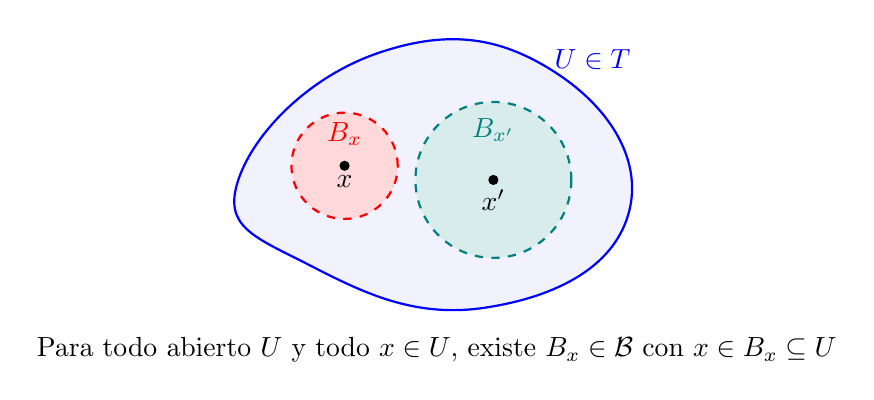
\begin{tikzpicture}[scale=0.9]
    % Abierto U grande
    \draw[thick,blue,fill=blue!5] plot[smooth cycle,tension=0.8] coordinates {(0,0) (2,1.8) (4.5,1.5) (5.5,-0.5) (3.5,-1.8) (1,-1.2)};
    \node[blue] at (5,1.7) {\(U \in \mc T\)};
    
    % Elementos basicos B_x alrededor de puntos
    \draw[thick,red,dashed,fill=red!15] (1.5,0.2) circle (0.75cm);
    \filldraw[black] (1.5,0.2) circle (1.8pt) node[below] {\(x\)};
    \node[red] at (1.5,0.65) {\(B_x\)};
    
    \draw[thick,teal,dashed,fill=teal!15] (3.6,0) circle (1.1cm);
    \filldraw[black] (3.6,0) circle (1.8pt) node[below] {\(x'\)};
    \node[teal] at (3.6,0.7) {\(B_{x'}\)};
    
    \node at (2.8,-2.4) [align=center] {Para todo abierto \(U\) y todo \(x \in U\), existe \(B_x \in \mathcal{B}\) con \(x \in B_x \subseteq U\)};
\end{tikzpicture}
\end{center}

\begin{ejem}
En \((\mathbb{R}, \mc T_d)\):
\begin{itemize}
    \item \(\mathcal{B} = \{B_d(x, \varepsilon) \mid x \in \mathbb{R}, \; \varepsilon > 0\}\) es base.
    \item \(\mathcal{B}_1 = \{(a, b) \mid a < b, \; a, b \in \mathbb{R}\}\) es base.
    \item \(\mathcal{B}_2 = \{(a, b) \mid a < b, \; a, b \in \mathbb{Q}\}\) es base numerable de \(\mc T_d\). Nótese que \(\mathcal{B}_2 \subsetneq \mathcal{B}_1\).
    \item \(\mathcal{B}_3 = \{(a, b) \mid a, b \in \mathbb{R} \setminus \mathbb{Q} = \bb I \}\) es también base.
\end{itemize}
\end{ejem}
Sea $X$ un conjunto
\begin{teo}
Un subconjunto \(\mathcal{B} \subseteq \mathcal{P}(X)\) es base de una topología \(\mc T\) en \(X\) de la cual \(\mathcal{B}\) es base si y solo si \(\mathcal{B}\) satisface:
\begin{enumerate}
    \item[\textbf{1)}] Para todo \(x \in X\), existe \(B_x \in \mathcal{B}\) tal que \(x \in B_x\) (es decir, \(\bigcup_{B \in \mathcal{B}} B = X\)).
    \item[\textbf{2)}] Dados \(B_1, B_2 \in \mathcal{B}\), para cada \(x \in B_1 \cap B_2\) existe \(B_x' \in \mathcal{B}\) tal que \(x \in B_x' \subseteq B_1 \cap B_2\).
\end{enumerate}
Dicha topología \(\mc T\) es única y es $\mc T = <\mc B>$.
\end{teo}

\begin{dem} \, 
\begin{itemize}
    \item[(\(\Rightarrow\))] Sea \(\mc T\) una topología en \(X\) y sea \(\mathcal{B}\) una base de \(\mc T\).
    \begin{itemize}
        \item Como \(X \in \mc T\), para cada \(x \in X\) existe \(B_x \in \mathcal{B}\) tal que \(x \in B_x \subseteq X\). Luego se cumple 1.
        \item Sean \(B_1, B_2 \in \mathcal{B} \subseteq \mc T\). Por ser \(\mc T\) topología, \(B_1 \cap B_2 \in \mc T\). Al ser \(B_1 \cap B_2\) un abierto y \(\mathcal{B}\) base, para cada \(x \in B_1 \cap B_2\) existe \(B_x' \in \mathcal{B}\) tal que \(x \in B_x' \subseteq B_1 \cap B_2\). Luego se cumple 2.
    \end{itemize}
    \item[(\(\Leftarrow\))] Sea $\mc B \subset \mc P(X)$ verificando 1) y 2), se define la familia:
    \[
        \mc T \coloneqq \{U \subseteq X \mid \forall x \in U, \; \exists B_x \in \mathcal{B} \text{ con } x \in B_x \subseteq U\} \text{}.
    \]
    Veamos que \(\mc T\) es una topología en \(X\):
    \begin{enumerate}
        \item[\textbf{a)}] \(\emptyset \in \mc T\) por definición de $\mc T$. Por la condición 1, para cada \(x \in X\) existe \(B_x \in \mathcal{B}\) con \(x \in B_x \subseteq X\), luego \(X \in \mc T\).
        \item[\textbf{b)}] Sean \(U_1, \ldots, U_n \in \mc T\) y sea \(x \in U_1 \cap \cdots \cap U_n\). Como \(x \in U_i\, \forall i, \ldots, n\), existe \(B_i \in \mathcal{B}\) con \(x \in B_i \subseteq U_i\). Entonces \(x \in B_1 \cap \cdots \cap B_n \subset U_1 \cap \cdots \cap U_n\). Por la condición 2, existe \(B \in \mathcal{B}\) tal que:
        \[
            x \in B \subseteq B_1 \cap \cdots \cap B_n \subseteq U_1 \cap \cdots \cap U_n \text{}.
        \]
        Por consiguiente, \( U_1 \cap \cdots \cap U_n \in \mc T\).
        \item[\textbf{c)}] Sea \(\{U_i\}_{i \in I} \subseteq \mc T\) y sea \(x \in \bigcup_{i \in I} U_i\). Existe \(i_0 \in I\) tal que \(x \in U_{i_0}\). Como \(U_{i_0} \in \mc T\), existe \(B_x \in \mathcal{B}\) tal que:
        \[
            x \in B_x \subseteq U_{i_0} \subseteq \bigcup_{i \in I} U_i \text{}.
        \]
        Por consiguiente, \( \displaystyle \bigcup_{i \in I} U_i \in \mc T\).
    \end{enumerate}
    Así, \(\mc T\) es una topología en \(X\). Además, \(\mathcal{B} \subseteq \mc T\) (tomando \(B_x = B\) para cada \(x \in B\)), y por la propia definición de \(\mc T\), \(\mathcal{B}\) es base de \(\mc T\).
    
    \item[\textbf{Unicidad:}] Si existiera otra topología \(\mc T'\) con base \(\mathcal{B}\), todo abierto de \(\mc T'\) sería unión de elementos de \(\mathcal{B}\) (que pertenecen a \(\mc T\)), luego \(\mc T' \subseteq \mc T\). Recíprocamente, todo abierto de \(\mc T\) es unión de elementos de \(\mathcal{B} \subseteq \mc T'\), luego \(\mc T \subseteq \mc T'\), concluyendo que \(\mc T = \mc T'\).
\end{itemize}
\end{dem}

\begin{obs}
La condición 2 del teorema es equivalente a exigir que para cualesquiera \(B_1, \ldots, B_n \in \mathcal{B}\) y para cada \(x \in \bigcap_{k=1}^n B_k\), existe \(B_x \in \mathcal{B}\) con \(x \in B_x \subseteq \bigcap_{k=1}^n B_k\).
\end{obs}

\begin{dem}
Para \(n = 2\) es la propia condición 2. Supongamos cierto para \(n-1\): si \(x \in \bigcap_{k=1}^n B_k\), entonces \(x \in (\bigcap_{k=1}^{n-1} B_k) \cap B_n\). Por hipótesis de inducción, existe \(B_x^{n-1} \in \mathcal{B}\) con \(x \in B_x^{n-1} \subseteq \bigcap_{k=1}^{n-1} B_k\). Entonces \(x \in B_x^{n-1} \cap B_n\), y aplicando el caso \(n=2\) existen \(B_x \in \mathcal{B}\) con \(x \in B_x \subseteq B_x^{n-1} \cap B_n \subseteq \bigcap_{k=1}^n B_k\).
\end{dem}

\begin{ejer}[Topología de Sorgenfrey o del límite inferior]
En \(\mathbb{R}\), consideremos la familia de intervalos semiabiertos \(\mathcal{B} = \{[a, b) \mid a < b, \; a, b \in \mathbb{R}\} \subset \mathcal{P}(\mathbb{R})\). Se verifican las condiciones del teorema
\begin{enumerate}
    \item[\textbf{1)}] Para todo \(x \in \mathbb{R}\), \(x \in [x, x+1) \in \mathcal{B}\).
    \item[\textbf{2)}] Dados \([a, b), [a', b') \in \mathcal{B}\), su intersección es:
    \[
        [a, b) \cap [a', b') = \begin{cases} \emptyset & \text{si } \max\{a, a'\} \ge \min\{b, b'\}, \\ [\max\{a, a'\}, \min\{b, b'\}) \in \mathcal{B} & \text{si } \max\{a, a'\} < \min\{b, b'\}. \end{cases} \text{}
    \]
\end{enumerate}
Por tanto, \(\mathcal{B}\) es base de una topología en \(\mathbb{R}\), denotada \(\mc T_{\text{Sorg}}\) (o \(\mathbb{R}_l\)). Se verifica que \(\mc T_d \subsetneq \mc T_{\text{Sorg}}\), puesto que todo intervalo abierto usual es unión de intervalos de \(\mathcal{B}\):
\[
    (a, b) = \bigcup_{n=1}^\infty \left[a + \frac{1}{n}, b\right) \in \mc T_{\text{Sorg}} \text{},
\]
mientras que \([a, b) \notin \mc T_d\).
\end{ejer}
Sabemos que $\mc T_d=<\mc B>$, siendo $\mc B=\{(a,b), \, / \,  a,b \in \bb R\}$. Si demostramos que $\mc B \subset \mc T_{Sorg}\Rightarrow <\mc B>=\mc T_d \subseteq \mc T_{Sorg}$ (\textbf{Observaci\'on:} La diferencia entre $\mc B$ y $<\mc B>$ es que en $<\mc B>$ est\'an las uniones arbitrarias). 

Sea $(a,b)\in \mc T_d$ veamos si $(a,b)\in \mc T_{Sorg} \iff \forall \, x\in (a,b) \, \exists \, B_x\subset \mc B_{Sorg}\, / \, x\in B_x \subset(a,b)$. Queremos encontrar un intervalo de la forma $[\,\,)$ que contenga a $x$ y est\'e contenido en $(a,b)$. 

Sea $x\in (a,b) \Rightarrow x\neq b \Rightarrow b-x = \varepsilon'>0, \, \varepsilon = \frac{\varepsilon}{2}$. As\'i $[x,x+\varepsilon)=B\subset (a,b)$ es el intervalo que busc\'abamos ya que $x\in B \subset(a,b)$. 

Por tanto, $[a,b) \in \mc T_{Sorg}$ pero $[a,b)\nin \mc T_d$.

Para la otra inclusi\'on basta ver que no se cumple si encontramos un elementos de $\mc T_{Sorg}$ que no est\'a en $\mc T_d$ (trivial). 
\begin{ejer}
Si $\mc B$ es base de una topolog\'ia en $X$, entonces $<\mc B>$ es la menor topolog\'ia de $X$ que contiene a $\mc B$.
\end{ejer}
\begin{ejer}
Ya sabemos que $\mc T_d\subset \mc T_{Sorg}$ y que $[a,b)\in \mc T_{Sorg}$. ¿$(-\infty,a), (-\infty,a], (b,\infty), [b,\infty)$ son abiertos, cerrados o ambos por la $\mc T_{Sorg}$? 
\begin{itemize}
    \item $(-\infty, a) \in \mc T_d \Rightarrow (-\infty, a) \in \mc T_{Sorg}$ pues $\mc T_d\subset \mc T_{Sorg}$
    \item $(-\infty,a]$. $\forall \, x\in (-\infty,a] \, \exists [\,\,)\, / \, x\in [\,\,) \subset(-\infty,a]?$
    
    Para $a\in (-\infty,a], \, [a,a+\varepsilon) \nsubseteq (-\infty,a]\Rightarrow $ no abierto.
    \item $(b,\infty) \in \mc T_d \Rightarrow (b,\infty)\in \mc T_{Sorg}$.
    \item $[b,\infty)\, \forall \, x\in [b,\infty)\, \exists\,[x,x+1) \, / \, x \in [x,x+1) \subset [b, \infty) \Rightarrow $ es abierto.
    
    Veamos si son cerrados
    \item  $(-\infty,a)^c=[a,\infty)$ es abierto para $\mc T_S \Rightarrow (-\infty,a)$ es cerrado.
    \item $(-\infty,a]^c = (a,\infty)$ es abierto para $\mc T_S \Rightarrow (-\infty,a]$ es cerrado.
    \item $(b,\infty)^c = (-\infty,b]$ no abierto $\Rightarrow (b,\infty)$ no cerrado.
    \item $[b,\infty)^c = (-\infty, b)$ es abierto $\Rightarrow [b,\infty)$ es cerrado.
\end{itemize}
Tenemos pues, por definici\'on, $[a,b)$ son abiertos para $\mc T_{Sorg}$. Sus complementarios son $(-\infty,a) \cup [b,\infty)$ abiertos por ser ambos abiertos, luego $[a,b)$ son cerrados. 

\underline{Conclusi\'on}: $[a,b)$ son abiertos y cerrados.

En cambio, $(a,b]$ no es abierto para $\mc T_{Sorg}$ pues $(a,b]^c = \underbrace{(-\infty,a]}_{no \, ab.}\cup \underbrace{(b,\infty)}_{ab.}$ no es abierto, debido al punto $a\in (-\infty,a]\cup [b,\infty)$ (NO porque no ab $\cup$ ab no sea abierto, lo podr\'ia llegar ser).

\underline{Conclusi\'on}: $(a,b]$ no son abiertos ni cerrados.
\end{ejer}
\begin{ejer}
    Sean $\mc T \subset \mc T'$ dos topolog\'ias en $X$, entonces todo abierto por $\mc T$ es abierto por $\mc T'$. Demostrar que si $C \subset X$ es cerrado por $\mc T$, entonces es cerrado por $\mc T'$. 
\end{ejer}
\begin{sol}
Si $C$ cerrado por $\mc T$, $C^c = U= X-C$ abierto por $\mc T$, como $\mc T \subset \mc T'$, $U \in \mc T \subset \mc T' \Rightarrow U = C^c \in \mc T'$ por lo que su complementario $C$ es cerrado en $\mc T'$.  OJO: $\mc P(X) - \mc T \neq \mc C_{\mc T}$
\end{sol}
\section{Topología por cerrados}

Sea \((X, \mc T)\) un espacio topológico. La familia de cerrados se define como \(\mathcal{C}_\mc T \coloneqq \{X \setminus U \mid U \in \mc T\} \subseteq \mathcal{P}(X)\), es decir, el conjunto de los complementarios de los abiertos de la topología $\mc T$.

\begin{prop}
La familia \(\mathcal{C}_\mc T\) verifica las siguientes propiedades:
\begin{enumerate}
    \item[\textbf{1)}] \(\emptyset, X \in \mathcal{C}_\mc T\).
    \item[\textbf{2)}] Si \(C_1, \ldots, C_n \in \mathcal{C}_\mc T \Rightarrow C_1 \cup \ldots \cup C_n \in \mathcal{C}_\mc T\) (uniones finitas de cerrados son cerradas).
    \item[\textbf{3)}] Si \(\{C_i\}_{i \in I} \subseteq \mathcal{C}_\mc T \Rightarrow \bigcap_{i \in I} C_i \in \mathcal{C}_\mc T\) (intersecciones arbitrarias de cerrados son cerradas).
\end{enumerate}
\end{prop}

\begin{dem}
\begin{enumerate}
    \item[\textbf{1)}] \(\emptyset = X \setminus X\) con \(X \in \mc T\), y \(X = X \setminus \emptyset\) con \(\emptyset \in \mc T\), luego \(\emptyset, X \in \mathcal{C}_\mc T\).
    \item[\textbf{2)}] Sean \(C_1, \ldots, C_n \in \mathcal{C}_\mc T\). Existen \(U_1, \ldots, U_n \in \mc T\) tales que \(C_k = X \setminus U_k\). Por las leyes de De Morgan:
    \[
        \bigcup_{k=1}^n C_k = \bigcup_{k=1}^n (X \setminus U_k) = X \setminus \left(\bigcap_{k=1}^n U_k\right) \text{}.
    \]
    Como \(\mc T\) es topología, \(\bigcap_{k=1}^n U_k \in \mc T\), y su complementario pertenece a \(\mathcal{C}_\mc T\).
    \item[\textbf{3)}] Sea \(\{C_i\}_{i \in I} \subseteq \mathcal{C}_\mc T\), con \(C_i = X \setminus U_i\) para \(U_i \in \mc T\). Por las leyes de De Morgan:
    \[
        \bigcap_{i \in I} C_i = \bigcap_{i \in I} (X \setminus U_i) = X \setminus \left(\bigcup_{i \in I} U_i\right) \text{}.
    \]
    Como \(\bigcup_{i \in I} U_i \in \mc T\), su complementario pertenece a \(\mathcal{C}_\mc T\).
\end{enumerate}
\end{dem}
\begin{obs}
    Para ciertas topolog\'ias es mucho m\'as c\'omodo hablar en t\'erminos de cerrados.
    \begin{itemize}
        \item $\mc C_{\mc T_{cof}} = \{A\subset X \, / \, A \text{ es finito}\} \cup \{X\}$
        \item $\mc C_{\mc T_{cocont}} = \{A\subset X \, / \, A \text{ es contable}\} \cup \{X\}$
    \end{itemize}
\end{obs}
\begin{ejem}
\begin{enumerate}
    \item Sea $X=\{a,b,c\}$ nuestro conjunto, si $\mc T=\{\emptyset, X, \{a\},\{b,c\}\}$ es nuestra topolog\'ia por abiertos de $X$, $\mc C_{\mc T} = \{X, \emptyset,\{b,c\},\{a\}\}$ es nuestra topol\'ia por cerrados.
    
    En $(X,\mc T)$ los abiertos y cerrados son los mismos subconjuntos y hay subconjuntos que no son ni abiertos ni cerrados, como por ejemplo $\{a,b\}$.
    \item Sea $(\bb R, \mc T_d)$,
    \begin{itemize}
        \item $(a,b) \in \mc T_d$
        \item $[a,b] \in \mc C_{\mc T_d}$ pues $\bb R - [a,b] = (-\infty,a) \cup(b,\infty) \in \mc T_d$. Adem\'as, $[a,b]\nin \mc T_d$ pues tomando $a\in [a,b] \, \nexists \, B(a, \varepsilon) \subset [a,b]$.
        \item Por tanto, $ [a,b],[a,b),(a,b] \nin \mc T_d$
        \item Adem\'as, haciendo complementarios $(a,b] \nin \mc C_{\mc T_d}, \, [a,b) \nin \mc C_{\mc T_d}, \, (-\infty, a] \nin \mc C_{\mc T_d}$
        \item $\{0\}^c=(-\infty,0) \cup (0,\infty) \Rightarrow 0 \in \mc C_{\mc T_d}$ es decir, que el complementario de cualquier $x\in \bb R$ es uni\'on de dos abiertos, por lo tanto abierto, y esto nos dice que $\{x\}$ es cerrado en $(\bb R, \mc T_d)$.
    \end{itemize}
\end{enumerate}
\end{ejem}

\begin{teo}
Sea \(X\) un conjunto y sea \(\mathcal{C} \subseteq \mathcal{P}(X)\) una familia de subconjuntos. Existe una (única) topología \(\mc T\) por abiertos en \(X\) tal que \(\mathcal{C}_\mc T = \mathcal{C}\) si y solo si \(\mathcal{C}\) satisface las condiciones 1, 2 y 3 de la proposición anterior.
\end{teo}

\begin{dem}
Si \(\mathcal{C}\) verifica las tres condiciones, definiendo \(\mc T \coloneqq \{X \setminus C \mid C \in \mathcal{C}\}\), al tomar complementarios las tres condiciones de \(\mathcal{C}\) se traducen directamente (por De Morgan) en los tres axiomas de topología por abiertos de la Definición 1.1.
\end{dem}

\begin{defi}
Sea \((X, \mc T)\) un espacio topológico y \(\mathcal{C}\) su familia de cerrados. Una subfamilia \(\mathcal{B}_{\text{cerr}} \subseteq \mathcal{C}\) es una \textbf{base de cerrados} si para todo cerrado \(C \in \mathcal{C}\) y todo punto \(x \notin C\), existe un elemento básico \(B_x \in \mathcal{B}_{\text{cerr}}\) tal que:
\[
    C \subseteq B_x \quad \text{y} \quad x \notin B_x \text{}.
\]
Equivalentemente, todo cerrado \(C \in \mathcal{C}\) es intersección de elementos de \(\mathcal{B}_{\text{cerr}}\): \(C = \bigcap_{i \in I} B_i\) con \(B_i \in \mathcal{B}_{\text{cerr}}\).
\end{defi}

\begin{center}
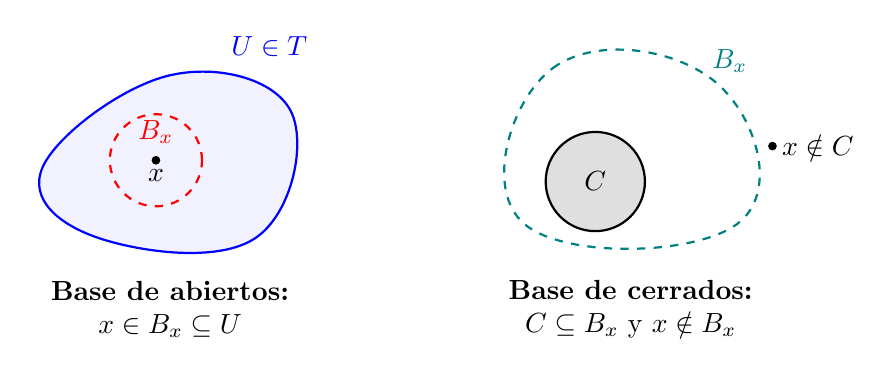
\begin{tikzpicture}[scale=0.9]
    % Base por abiertos
    \begin{scope}[shift={(0,0)}]
        \draw[thick,blue,fill=blue!5] plot[smooth cycle,tension=0.7] coordinates {(0,0) (1.8,1.3) (3.5,0.8) (3,-1) (0.8,-1)};
        \node[blue] at (3.2,1.7) {\(U \in \mc T\)};
        \draw[thick,red,dashed] (1.6,0.1) circle (0.65cm);
        \filldraw[black] (1.6,0.1) circle (1.5pt) node[below] {\(x\)};
        \node[red] at (1.6,0.5) {\(B_x\)};
        \node at (1.8,-2) [align=center] {\textbf{Base de abiertos:} \\ \(x \in B_x \subseteq U\)};
    \end{scope}
    
    % Base por cerrados
    \begin{scope}[shift={(7,0)}]
        \draw[thick,fill=gray!25] (0.8,-0.2) circle (0.7cm);
        \node at (0.8,-0.2) {\(C\)};
        \draw[thick,teal,dashed] plot[smooth cycle,tension=0.8] coordinates {(-0.2,-0.8) (0.2,1.4) (2.5,1.2) (2.8,-0.8)};
        \node[teal] at (2.7,1.5) {\(B_x\)};
        \filldraw[black] (3.3,0.3) circle (1.5pt) node[right] {\(x \notin C\)};
        \node at (1.3,-2) [align=center] {\textbf{Base de cerrados:} \\ \(C \subseteq B_x\) y \(x \notin B_x\)};
    \end{scope}
\end{tikzpicture}
\end{center}

\section{Subbases de una topología}

\begin{defi}
Un subconjunto \(S\mc B \subseteq \mathcal{P}(X)\) es una \textbf{subbase} de una topología en \(X\) si cubre a \(X\): para todo \(x \in X\) existe \(S \in S\mathcal{B}\) tal que \(x \in S\) (\(X = \bigcup_{S \in S\mathcal{B}} S\)).
\end{defi}

La base generada por \(S\mathcal{B}\) es la familia de todas las intersecciones finitas:
\[
    S\mc B \subset \mathcal{B}_{S\mathcal{B}} = \{B\subset X \, / \, B=S_1 \cap \ldots \cap S_n \mid S_j \in S\mathcal{B}, \; n \in \mathbb{N}\} \text{},
\]
base de una topolog\'ia y la topología generada por \(S\mathcal{B}\) es:
\[
    \mc T_{S\mathcal{B}}  = \mc T_{\mc B_{S\mc B}} = <\mc B_{S\mc B}> = \left\{\bigcup_{j \in J} (V_{j, 1} \cap \ldots \cap V_{j, n_j}) \;\middle|\; V_{j, r} \in \mathcal{S}\right\} \cup \{\emptyset\} \text{}.
\] es decir, las uniones arbitrarias de intersecciones finitas de elementos de $S\mc B$. 

\begin{ejem}
En \(\mathbb{R}\):
\begin{itemize}
    \item \(S\mathcal{B} \coloneqq \{(-\infty, b), (a, \infty) \mid a, b \in \mathbb{R}\}\) es subbase de la topología usual \(\mc T_d\): para cada \(x \in \mathbb{R}\), \(x \in (x - 1, \infty) \in \mathcal{S}\). Además, \((a, b) = (-\infty, b) \cap (a, \infty) \in \mathcal{B}_{S\mathcal{B}}\), lo que genera la base de intervalos usual y demuestra que \(\mc T_{S\mathcal{B}} = \mc T_d\).
    \item \(S\mathcal{B}' \coloneqq \{(-\infty, b], [a, \infty) \mid a, b \in \mathbb{R}\}\) es subbase de la topología discreta \(\mc T_{\text{discreta}}\), ya que considerando $x \in \bb R$ buscamos un abierto de la subbase que lo contenga \(\{x\} = (-\infty, x] \cap [x, \infty) \in \mathcal{B}_{S\mathcal{B}'}\), haciendo que todos los conjuntos unitarios sean abiertos, lo que demuestra que $<S\mc B'>= \mc T_{disc}$. Pues $Y = \displaystyle \bigcup_{y\in Y} \{y\}$ cada subconjunto es uni\'on de sus puntos.
\end{itemize}
\end{ejem}

\section{Bases y subbases de una topolog\'ia por cerrados}
Todas las demostraciones son pasando al complementario.

Sea $(X,\mc C)$ esapcio topol\'ogico por cerrados. \begin{defi}
    $\mc B \subset \mc P(X)$ es un \textbf{base por cerrados} (o \textbf{base de $\mc C$}) si para todo cerrado $C$ y para todo $x\nin C$, existe $B \in \mc B$ tal que $x\nin B \supset C \iff X \neq C =\displaystyle \bigcap_{B_i \in \mc B} B_i$, es decir, todo cerrado es intersecci\'on de cerrados de la base. 
\end{defi}
\begin{defi} La base $\mc B$ genera una topolog\'ia por abiertos 
    $$\mc C_{\mc B} = <\mc B> = \{C \subset X \, / \, \forall x \nin C, \text{ existe } B_x \in \mc B \, / \, x \nin B_x \supset C\}  =\left\{\bigcap_{B_i \in \mc B} B_i \right\}\cup \{X\}$$
    Los cerrados de una base de $\mc C$ se llaman \textbf{cerrados básicos}, y son los complementarios de los abiertos b\'asicos.

\end{defi}
\begin{prop}
Si $X$ es conjunto, $\mc B \subset \mc P(X)$, $\mc B$ es una base por cerrados si y solo si
\begin{enumerate}
    \item $\forall\, x\in X$, existe $b\in \mc B$ tal que $x\nin B$.
    \item $\forall \, B_1,B_2 \in \mc B$ y para todo $x \in B_1\cup B_2$, existe $B_x \in \mc B$ tal que $x \nin B_x \supseteq B_1 \cup B_2$.
\end{enumerate}
\end{prop}
\begin{defi}
    Una \textbf{subbase por cerrados} $S\mc B$ es un subconjunto $S\mc B\subset \mc P(X)$ que verifica 
    \begin{enumerate}
        \item $\forall \, x\in X$, existe $S\in S\mc B$ tal que $x\nin S$. $\mc B_{S\mc B}$
        \item $<\mc B_{S\mc B}> = \mc T_{S\mc B}$ con $\mc B_{S\mc B} \coloneqq \{S_1\cup \cdots \cup S_n \, / \,S_i\in S\mc B \}$, es decir, son uniones finitas de intersecciones arbitrarias. 
    \end{enumerate}
\end{defi}
\section{Elementos de un espacio topol\'ogico}
Sea $X$ un espacio topol\'ogico y sea $Y\subseteq X$ un subconjunto
\begin{defi} El \textbf{interior} de un subconjunto $Y\subset X$ es el mayor abierto de $X$ contenido en $Y$:
    $$Y^{\circ} = \{y\in Y \, / \, \text{ existe un abierto } U_y \text{ tal que } y\in U_y \subset Y\} = \bigcup_{U\subset Y} U$$
    Siempre existe $\emptyset$ lo verifica y es abierto en $X$. Adem\'as, si $V \subseteq X$ es abierto, $V\subset Y \Rightarrow V \subseteq Y^{\circ}$.
\end{defi}
\begin{defi}
El \textbf{cierre} (o \textbf{clausura} o \textbf{adherencia}) de un subconjunto $Y \subseteq X$ es el menor cerrado de $X$ que contiene a $Y$:
\[
    \overline{Y} \coloneqq \bigcap_{\substack{Y \subseteq C \\ C \in \mathcal{C}_\mc T}} C.
\]
Se cumple que $Y \subseteq \overline{Y}$. 
\end{defi}
\begin{prop}
\[
    \overline{Y} = \{x \in X \mid \text{ para todo abierto } U_x \ni x \text{ se verifica que } U_x \cap Y \ne \emptyset\}.
\]
\end{prop}
\begin{dem}
\begin{itemize}
    \item[($\subseteq$)] Sea $x \in \overline{Y}$ y sea $U_x$ un abierto con $x \in U_x$. Supongamos que $U_x \cap Y = \emptyset$. Entonces $Y \subseteq X \setminus U_x$. Como $X \setminus U_x$ es cerrado, por definición de cierre $\displaystyle \overline{Y} = \bigcap_{\substack{C' cualquiera \\ C' \supset Y}} C ' \subseteq C' \Rightarrow x \in X \setminus U_x$, contradiciendo que $x \in U_x$. Por tanto, $U_x \cap Y \ne \emptyset$.
    \item[($\supseteq$)] Veamos que $x\in \overline Y = \bigcap C \iff x\in C \, / \, \forall C \supset Y$. Sea $C$ cerrado, $C\supset Y$ y supongamos que $x\nin C \Rightarrow x \in X-C = U$ abierto. Como $Y\subset C$, $X-C \cap Y=\emptyset$. Por definci\'on del cierre, $U\cap Y = \emptyset$ llegando a contradicci\'on, al suponer que $x\nin C$.
\end{itemize}
\end{dem}
\begin{defi}
    Sea $Y\subset X$, se llaman \textbf{puntos de acumulación} al subconjunto:
    $$Y' = \{x\in X \mid \text{para todo abierto } U_x \text{ con } x\in U_x, \, U_x \cap Y \neq \emptyset, \{x\}\}$$

\end{defi}
\begin{obs}
    $Y' \subset \overline{Y}$ (ejercicio).
\end{obs}
\begin{defi}Se definen los \textbf{puntos aislados} de $Y$ como
    $$Y^a = \{y\in Y \mid \text{ existe un abierto } U_y, y\in U_y \text{ tal que } U_y \cap Y = \{y\} \} = \{y \in Y \mid y \in Y'\}\subset Y$$
\end{defi}
\begin{defi}
    Se define la \textbf{frontera} de $Y$ como 
    $$Fr(Y) = \overline{Y} \cap \overline{(X-Y)}$$
\end{defi}
\begin{defi}
    Se define el \textbf{borde} de $Y$ como 
    $$b(Y) = Y \cap Fr(Y) = Y \cap \overline{(X-Y)}$$ 
\end{defi}
\begin{defi}
    Se define el \textbf{exterior} de $Y$ como 
    $$Ext(Y)=(X-Y)^{\circ}$$
\end{defi}
\begin{propis}
\begin{enumerate}
    \item $\overline{Y} = Y \cup Y' = Y^a \sqcup Y'$
    \begin{dem}
        $\subseteq) $ Sea $x\in \overline{Y}$, 

        Si $x\in Y$, hemos acabado.

        Si $x\nin Y$, por ser $x\nin \overline{Y} \Rightarrow \forall\, U_x$ abierto, $U_x\cap Y \neq \emptyset$ y $U_x\cap Y \neq x$ pues $x\nin Y \Rightarrow x\in Y' \Rightarrow x\in Y \cup Y'$

        $\supseteq)$ Como $Y \subset \overline{Y}$ y $Y' \subset \overline{Y} \Rightarrow Y \cup Y' \subset \overline{Y}$, luego
        $$Y\cap Y' = Y-Y^a \Rightarrow \overline{Y} = Y^a \cup Y' = Y^a \sqcup Y'$$
    \end{dem}
    \item $Y^{\circ} \cap b(Y) = \emptyset$
    \begin{dem}
        Sea $x\in Y^{\circ} \Rightarrow x \overset{?}{\nin} b(Y)$

        $x\in Y^{\circ} \Rightarrow$ existe $U_x$ abierto con $x\in U_x \subset Y \Rightarrow x\nin b(Y) \Rightarrow Y^{\circ} \cap b(Y) = \emptyset$
    \end{dem}
    \item $Y^{\circ} \cap Fr(Y) = \emptyset$ (se deduce de lo anterior)
    
    $Y^{\circ} \cap b(Y)  = Y^{\circ} \cap Fr(Y)$ porque $Y^{\circ} \subseteq Y$.
\end{enumerate}
\end{propis}



\begin{ejem}
En $(\mathbb{R}, \mc T_d)$, sea $Y = [0, 1)$:
\begin{itemize}
    \item $Y^\circ = (0, 1)$, $\overline{Y} = [0, 1]$, $Y' = [0, 1]$, $Y^a = \emptyset$.
    \item $X \setminus Y = (-\infty, 0) \cup [1, \infty)$, $\overline{X \setminus Y} = (-\infty, 0] \cup [1, \infty)$.
    \item $\operatorname{Fr}(Y) = \{0, 1\}$.
    \item $b(Y) = \{0\}$.
    \item $\operatorname{Ext}(Y) = (-\infty, 0) \cup (1, \infty)$.
\end{itemize}
\end{ejem}

\begin{ejem}
En $\mathbb{R}^2$ con la topología usual, sea $Y = [1, 3) \times [1, 2) \cup \{(4, 1), (5, 1)\}$:
\begin{itemize}
    \item $Y^\circ = (1, 3) \times (1, 2)$.
    \item $\overline{Y} = [1, 3] \times [1, 2] \cup \{(4, 1), (5, 1)\}$.
    \item $Y' = [1, 3] \times [1, 2]$.
    \item $Y^a = \{(4, 1), (5, 1)\}$.
\end{itemize}
\end{ejem}
\begin{prop}
    $Y$ es cerrado $\iff Fr(Y) \subset Y$.
\end{prop}
\begin{dem}
    $\Rightarrow) \, Y$ cerrado $\Rightarrow Y = \bar Y \supset Fr(Y) \Rightarrow Fr(Y) \subset Y$

    $\Leftarrow)$ Sabemos que $\bar Y = Y^{\circ} \sqcup Fr(Y)\subset Y$ (pues $Y^{\circ}, Fr(Y)\subset Y$). Luego
    $$\overline{Y} = Y^{\circ} \sqcup Fr(Y) \subset Y \subset \overline{Y} \Rightarrow Y = \overline{Y} \Rightarrow Y \text{ es cerrado.}$$
\end{dem}

\section{Propiedades fundamentales de los operadores}

\begin{propi}
Sean $X$ un espacio topológico e $Y \subseteq X$. Se verifican:
\begin{enumerate}
    \item[\textbf{I.}] $Y^\circ \cap \operatorname{Fr}(Y) = \emptyset$.
    \item[\textbf{II.}] $\operatorname{Ext}(Y) \cap \operatorname{Fr}(Y) = \emptyset$.
    \item[\textbf{III.}] $Y^\circ \cap b(Y) = \emptyset$.
    \item[\textbf{IV.}] $Y = Y^\circ \sqcup b(Y)$.
    \item[\textbf{V.}] $\overline{Y} = Y^\circ \sqcup \operatorname{Fr}(Y)$.
    \item[\textbf{VI.}] $Y$ es abierto $\iff b(Y) = \emptyset$.
    \item[\textbf{VII.}] $Y$ es cerrado $\iff \operatorname{Fr}(Y) \subseteq Y$.
    \item[\textbf{VIII.}] $\operatorname{Ext}(Y) = X \setminus \overline{Y}$.
    \item[\textbf{IX.}] $\overline{X \setminus Y} = X \setminus Y^\circ$.
    \item[\textbf{X.}] $\overline{Y^\circ} \subseteq \overline{Y}$ (en general no se da la igualdad).
    \item[\textbf{XI.}] $Y^\circ \subseteq (\overline{Y})^\circ$ (en general no se da la igualdad).
\end{enumerate}
\end{propi}

\begin{dem}
\begin{itemize}
    \item[\textbf{I.}] $Y^\circ \cap \operatorname{Fr}(Y) = Y^\circ \cap (\overline{Y} \cap \overline{X \setminus Y}) = Y^\circ \cap \overline{X \setminus Y} = \emptyset$, pues si $y \in Y^\circ$, existe un abierto $U_y \subseteq Y$, con lo cual $U_y \cap (X \setminus Y) = \emptyset$, lo que implica $y \notin \overline{X \setminus Y}$.
    \item[\textbf{II.}] $\operatorname{Ext}(Y) \cap \operatorname{Fr}(Y) = (X \setminus Y)^\circ \cap \operatorname{Fr}(X \setminus Y) = \emptyset$ aplicando la propiedad I a $X \setminus Y$.
    \item[\textbf{III.}] $Y^\circ \cap b(Y) = Y^\circ \cap (Y \cap \operatorname{Fr}(Y)) = Y^\circ \cap \operatorname{Fr}(Y) = \emptyset$.
    \item[\textbf{IV.}] Si $y \in Y$, o bien $y \in Y^\circ$, o bien para todo abierto $U \ni y$ se tiene $U \not\subseteq Y$, es decir, $U \cap (X \setminus Y) \ne \emptyset$, lo que implica $y \in \overline{X \setminus Y}$; luego $y \in Y \cap \overline{X \setminus Y} = b(Y)$. La unión es disjunta por III.
    \item[\textbf{V.}] Análoga a IV usando $\overline{Y}$ y $\operatorname{Fr}(Y)$.
    \item[\textbf{VI.}] $Y$ es abierto $\iff Y = Y^\circ \iff b(Y) = Y \setminus Y^\circ = \emptyset$.
    \item[\textbf{VII.}] $Y$ es cerrado $\iff X \setminus Y$ es abierto $\iff b(X \setminus Y) = \emptyset \iff (X \setminus Y) \cap \operatorname{Fr}(Y) = \emptyset \iff \operatorname{Fr}(Y) \subseteq Y$.
    \item[\textbf{VIII.}] $x \in \operatorname{Ext}(Y) \iff x \in (X \setminus Y)^\circ \iff \exists U_x \text{ abierto con } U_x \subseteq X \setminus Y \iff U_x \cap Y = \emptyset \iff x \notin \overline{Y} \iff x \in X \setminus \overline{Y}$.
    \item[\textbf{IX.}] Tomando complementarios en VIII: $\overline{X \setminus Y} = X \setminus (X \setminus (X \setminus Y))^\circ = X \setminus Y^\circ$.
    \item[\textbf{X.}] Como $Y^\circ \subseteq Y \Rightarrow \overline{Y^\circ} \subseteq \overline{Y}$. En $(\mathbb{R}, \mc T_d)$, para $\mathbb{Q}$ se tiene $\mathbb{Q}^\circ = \emptyset \Rightarrow \overline{\mathbb{Q}^\circ} = \emptyset \ne \mathbb{R} = \overline{\mathbb{Q}}$.
    \item[\textbf{XI.}] Como $Y^\circ$ es un abierto contenido en $Y \subseteq \overline{Y}$, necesariamente $Y^\circ \subseteq (\overline{Y})^\circ$. Para $\mathbb{Q}$ en $\mathbb{R}$: $\mathbb{Q}^\circ = \emptyset$, pero $(\overline{\mathbb{Q}})^\circ = \mathbb{R}^\circ = \mathbb{R}$.
\end{itemize}
\end{dem}

\section{Subconjuntos densos y clausura relativa}

\begin{defi}
Sea $X$ un espacio topológico e $Y \subseteq X$. Se dice que $Y$ es \textbf{denso} en $X$ si su cierre es el espacio total:
\[
    \overline{Y} = X.
\]
\end{defi}

\begin{prop}
Un subconjunto $Y \subseteq X$ es denso $\iff$ todo abierto no vacío $U \subseteq X$ corta a $Y$ ($U \cap Y \ne \emptyset$).
\end{prop}

\begin{dem}
($\Rightarrow$) Sea $U \ne \emptyset$ abierto en $X$. Sea $x \in U$. Como $X = \overline{Y}$, $x \in \overline{Y}$, por lo que todo entorno abierto de $x$ corta a $Y$; en particular, $U \cap Y \ne \emptyset$.

($\Leftarrow$) Sea $x \in X$. Todo abierto $U \ni x$ es no vacío, luego corta a $Y$, de donde $x \in \overline{Y}$. Por tanto, $X \subseteq \overline{Y} \Rightarrow \overline{Y} = X$.
\end{dem}

\begin{prop}
Sea $Y \subseteq X$ un subespacio topológico y sea $Z \subseteq Y$. Denotemos por $\overline{Z}^X$ la clausura de $Z$ en $X$. Entonces $Z$ es cerrado en $Y$ si y solo si:
\[
    Z = \overline{Z}^X \cap Y.
\]
\end{prop}

\begin{dem}
Si $Z$ es cerrado en $Y$, existe un cerrado $C \subseteq X$ tal que $Z = C \cap Y$. Como $Z \subseteq C$ y $C$ es cerrado en $X$, $\overline{Z}^X \subseteq C$. Por ende, $Z \subseteq \overline{Z}^X \cap Y \subseteq C \cap Y = Z$, de modo que $Z = \overline{Z}^X \cap Y$. El recíproco es inmediato, ya que $\overline{Z}^X$ es cerrado en $X$.
\end{dem}
\begin{ejem}
    $\bb Q$ es denso en $\bb R$.
\end{ejem}
\begin{ejem}
    Sea $(\bb R, \mc T_{kol})$, siendo $\mc T_{kol} = \{\emptyset, \bb R\} \cup \{(a,\infty), \, a \in \bb R\}$, consideremos $Y = \{0\} \cup [1,\infty)$. Tenemos que $\mc C_{\mc T_{kol}}= \{\emptyset, \bb R\} \cup\{(-\infty, a] , \, a\in \bb R\}$. Calculemos $Y$ aplicando operadores.
    \begin{itemize}
        \item $Y^{\circ} = (1, \infty)$. Por reducción al absurdo. Sea $b \in Y \subset (-\infty, a], b+(a-b)+2000 \in Y$ pero $b+(a-b)+2000 \nin (-\infty, a]$. 
        \item $X-Y = (-\infty, 0) \cup (0,1)$.
        \item $\overline{Y} = \bb R$. \textcolor{red}{TERMINAR DE CALCULAR EL RESTO}. 
    \end{itemize}
\end{ejem}



\section{Subespacios topol\'ogicos}

Sea \((X, \mc T_X)\) un espacio topológico y sea \(Y \subseteq X\) un subconjunto. Se tiene la aplicaci\'on inclusi\'on
$$\bt Y \rar[hook]{i} & X \\[-5mm] y \rarmaps & y \et$$
de forma que se induce la aplicaci\'on 
$$\bt \mc P(X) \rar[hook]{i^*} & \mc P(Y) &[-11mm] \\[-5mm]
 A \rarmaps & i^*(A) &[-12mm] = i^{-1}(A) = A \cap Y  \\[-5mm] 
 \mc T_X \rarmaps & i^*(\mc T_X) &[-11mm] = \{V \subset Y: \text{existe } &[-11mm] U \in \mc T_X \text{ tal que } i^*(U)=U\cap Y=V\} =:\mc T_X |_Y
\et$$
\begin{prop}
    $\mc T_X|_Y$ es una topolog\'ia en $Y$. 
\end{prop}\begin{dem}
    Por las propiedades de $i^*$. 
\end{dem}
\begin{defi}
Se tiene que $(Y, \mc T_X|_Y)$ es un espacio topol\'ogico, y decimos que $Y\subset (X,\mc T_X)$ es un \textbf{subespacio topológico} si en $Y$ tenemos la topolog\'ia $\mc T_X|_Y$. 
\end{defi}
\begin{defi}
    $V$ es \textbf{abierto en $Y$} si existe un abierto $U$ de $X$ tal que $U\cap Y = V$ (igual para cerrados por la intersecci\'on de complementarios). 
\end{defi}
\begin{obs}
    ¿Es $V$ abierto en $X$? Solo si $Y\subset X$ es abierto en $X$. Igual para cerrados. Diremos que abierto de abierto es abierto en el ambiente $X$ y cerrado de cerrado es cerrado en el ambiente. 
\end{obs}
\begin{ejer}
    Sea $Z \subset Y$, se verifica que $Z$ es cerrado si y solo si $\overline{Z^X} \cap Y = Z$.  
\end{ejer}
\begin{dem}
    (Nota: no es el \'unico cerrado que lo verifica pero es el menor cerrado de $X$ que lo verifica)

    $\Rightarrow) $ $Z$ cerrado en $Y \Rightarrow$ existe $C\subset X$ tal que $C\cap Y = Z \Rightarrow Z \subset C$ y como $Z \subset \overline{Z^X}$, $\overline{Z^X}\subset C \Rightarrow Z \cap Y = Z \subset \overline{Z^X} \cap Y \subset C \cap Y =Z\Rightarrow \overline{Z^X} \cap Y = Z$.
    
    $\Leftarrow)$ Existe $\overline{Z^X}$ cerrado en $X$ tal que $\overline{Z^X} \cap Y =Z \Rightarrow Z$ es cerrado en $Y$.
\end{dem}
\begin{prop}
    Un punto $y\in Y$ es \textbf{aislado en $Y$} $\iff \{y\} \subset Y$ es abierto en $Y$.
\end{prop}
\begin{dem}
    $y \in Y$ es aislado en $Y \,\iff \, $ existe un abierto $U \subset X$ tal que $U\cap Y = \{y\} \iff \{y\}$ es abierto en $Y$.
\end{dem}
\begin{prop}
    Sea $(X, \mc T_X)$ espacio topol\'ogico. Entonces un subconjunto $A\subset X$ es abierto en $X\, \iff \, $ para todo $x\in A$ existe un abierto $U_X \in \mc T_X$ tal que $x\in U_x\subset A \, \iff \, x\in A^{\circ} \, \forall \, x \in A \, \iff \, A = A^{\circ} \, \iff \, A \text{ es abierto. }$
\end{prop}

\section{Entornos}
\begin{defi}
Sea \((X, \mc T)\) un espacio topológico y sea \(x \in X\). Un subconjunto \(V \subseteq X\) es un \textbf{entorno} del punto \(x\) si existe un abierto \(U \in \mc T\) tal que:
\[
    x \in U \subseteq V \text{}.
\]
Denotamos la familia de entornos de \(x\) por \(\mathcal{E}_{\mc T_x}(x) = \{V \subseteq X \mid V \text{ es entorno de } x\} \subset \mc P (X)\).
\end{defi}

\begin{obs}
Un subconjunto \(W \subseteq X\) es abierto si y solo si es entorno de todos sus puntos. En efecto: si \(W\) es abierto, tomando \(U = W\) se tiene \(x \in W \subseteq W\). Recíprocamente, si \(W\) es entorno de cada \(x \in W\), existe un abierto \(U_x\) con \(x \in U_x \subseteq W\), luego \(\displaystyle W = \bigcup_{x \in W} U_x\) es abierto.
\end{obs}
Se denota $\{ \mc E(x)\}_{x \in X}$ a la familia de familias de entornos, que son subconjuntos.
\begin{teo}
Sea \((X, \mc T)\) un espacio topológico. Para cada \(x \in X\), la familia \(\mathcal{E}_\mc T(x)\) (\'o $\{ \mc E(x)\}_{x \in X}$) verifica:
\begin{enumerate}
    \item[\textbf{1)}] Si \(V \in \mathcal{E}_\mc T(x) \Rightarrow x \in V\).
    \item[\textbf{2)}] Si \(V_1, V_2 \in \mathcal{E}_\mc T(x) \Rightarrow V_1 \cap V_2 \in \mathcal{E}_\mc T(x)\).
    \item[\textbf{3)}] Si \(V \in \mathcal{E}_\mc T(x)\) y \(V \subseteq W \subseteq X \Rightarrow W \in \mathcal{E}_\mc T(x)\).
    \item[\textbf{4)}] Para cada \(V \in \mathcal{E}_\mc T(x)\), existe \(W \in \mathcal{E}_\mc T(x)\) tal que para todo \(y \in W\), \(V \in \mathcal{E}_\mc T(y)\).
\end{enumerate}
\end{teo}

\begin{dem}
\begin{enumerate}
    \item Si \(V \in \mathcal{E}_\mc T(x)\), por definición existe \(U \in \mc T\) con \(x \in U \subseteq V \Rightarrow x \in V\).
    \item Si \(V_1, V_2 \in \mathcal{E}_\mc T(x)\), existen \(U_1, U_2 \in \mc T\) con \(x \in U_1 \subseteq V_1\) y \(x \in U_2 \subseteq V_2\). Entonces:
    \[
        x \in U_1 \cap U_2 \subseteq V_1 \cap V_2 \text{}.
    \]
    Como \(U_1 \cap U_2 \in \mc T\), se deduce que \(V_1 \cap V_2 \in \mathcal{E}_\mc T(x)\).
     \item Si \(V \in \mathcal{E}(x)\) y \(W \subseteq X\) con \(V \subseteq W\), tenemos que existe \(U_x\) abierto tal que
    \[
        x \in U_x \subseteq V \subseteq W \Rightarrow W \in \mathcal{E}(x).
    \]
        \item Si \(V \in \mathcal{E}(x)\), existe \(U_x\) abierto tal que \(x \in \underbrace{U_x}_{\equiv W} \subseteq V \Rightarrow W \in \mathcal{E}(x)\) y \(W\) es abierto \(\Rightarrow\) es entorno de todos sus puntos,
    \[
        \forall y \in W : U_y = W \Rightarrow U_y = W \in \mathcal{E}(y) \Rightarrow V \in \mathcal{E}(y). \tag*{\(\blacksquare\)}
    \]
\end{enumerate}
\end{dem}
\begin{ejem}
    En $(\bb R, \mc T_d)$, $U \subset \bb R$ es abierto si para cada $x\in U$ existe $\varepsilon>0$ tal que $B(x,\varepsilon) \subset U$
    $$\mc E_{\mc T_d}(x) = \{V\subset \bb R : \text{ existe } \varepsilon>0 \text{ tal que } (x-\varepsilon, x+\varepsilon)\subset U\} = \{B_d(x, \varepsilon)\}``="\mc E_{\mc T_d}(x)$$
    se pone la \'ultima igualdad entre comillas pues las bolas son una base, y con estas se construyen todos los entornos, pero no es realmente una igualdad. 
\end{ejem}
\begin{obs}
        Comprobar cuando dé base de entornos \(\leftarrow\) Son una base, con esto construyes todos los entornos (no es realmente una igualdad). Para cada punto \(x\).
    \end{obs}
\begin{teo}
Sea \(X\) un conjunto y sea \(\{\mathcal{E}'(x)\}_{x \in X}\) una familia de subconjuntos de \(X\) asignada a cada punto \(x \in X\) que satisface los axiomas 1, 2, 3 y 4 anteriores. Entonces existe una \textbf{única} topología \(\mc T_{\{\mc E'(x)\}}\) en \(X\) tal que \(\{\mathcal{E}_{\mc T_{\{\mc E'(x)\}}}(x) \}= \{\mathcal{E}'(x)\}\) para todo \(x \in X\), donde $\mc T_{\{\mc E'(x)\}}=\{U\subset X \mid \text{ para todo } x\in U, U\in \mc E'(x)\}$.
\end{teo}

\begin{teo}
    Sea \(X\) un conjunto y para cada \(x \in X\), sea \(\mathcal{E}'(x) \subseteq \mathcal{P}(X)\). Para cada punto \(x \in X\), la familia \(\mathcal{E}'(x)\) verifica que:
    \begin{enumerate}
        \item Para todo \(V' \in \mathcal{E}'(x)\), \(x \in V'\).
        \item Si \(V_1', V_2' \in \mathcal{E}'(x)\), entonces \(V_1' \cap V_2' \in \mathcal{E}'(x)\).
        \item Si \(V' \in \mathcal{E}'(x)\) y \(W' \subseteq X\) es un subconjunto con \(V' \subseteq W'\), entonces \(W' \in \mathcal{E}'(x)\).
        \item Si \(V' \in \mathcal{E}'(x)\), entonces existe \(W' \in \mathcal{E}'(x)\) tal que para todo \(y \in W'\) se verifica que \(V' \in \mathcal{E}'(y)\).
    \end{enumerate}
    si y solo si existe una única topología en \(X\), \(\mc T_{(\mathcal{E}'(x))}\), tal que \(\{\mathcal{E}_{\mc T_{(\mathcal{E}'(x))}}(x)\}_{x \in X} = \{\mathcal{E}'(x)\}_{x \in X}\).
    
    Además, se verifica que
    \[
        \mc T_{(\mathcal{E}'(x))} = \{ U \subseteq X : \text{para todo } x \in U, \, U \in \mathcal{E}'(x) \}.
    \]
\end{teo}

\begin{dem} 
        \(\Rightarrow) \) Se verifica por el teorema anterior. Unicidad:
        \[
            \mathcal{E}_{\mc T_{(\mathcal{E}'(x))}}(x) = \mathcal{E}'(x) \quad \forall x \in X \quad (\mc T \text{ otra topología} \Rightarrow \text{son los mismos entornos} \] \[ \Rightarrow \text{mismos abiertos} \Rightarrow \text{misma topología}).
        \]
        
        \(\Leftarrow )\) Veamos que \(\mc T_{\mathcal{E}'}\) es topología por abiertos:
        \begin{enumerate}
            \item \(\emptyset \in \mc T_{\mathcal{E}'}\) por vacuidad (si el vacío no tiene puntos).
            
            \(X \in \mc T_{\mathcal{E}'}\), pues para cada \(x \in X\), sea \(V' \in \mathcal{E}'(x)\). Se tiene que \(\underbrace{x \in V'}_{(1)} \subseteq \underbrace{X \Rightarrow X \in \mathcal{E}'(x)}_{(3)}\), luego \(X \in \mc T_{\mathcal{E}'}\).
% ==========================================
% PÁGINA 8 (Continuación / Foto 2)
% ==========================================
            \item \(U_1, U_2 \in \mc T_{\mathcal{E}'} \stackrel{?}{\Rightarrow} U_1 \cap U_2 \in \mc T_{\mathcal{E}'}\).
            
            Sea \(x \in U_1 \cap U_2 \Rightarrow x \in U_1 \in \mc T_{\mathcal{E}'} \Rightarrow U_1 \in \mathcal{E}'(x)\), y como \(x \in U_2 \in \mc T_{\mathcal{E}'} \Rightarrow U_2 \in \mathcal{E}'(x)\) (por ser abiertos).
            
            Entonces \(U_1, U_2 \in \mathcal{E}'(x) \underset{(2)}{\Rightarrow} U_1 \cap U_2 \in \mathcal{E}'(x) \Rightarrow U_1 \cap U_2 \in \mc T_{\mathcal{E}'}\) (se verifica la definición para cada \(x\)).
            
            \item Sea \(\{U_i\}_{i \in I} \subseteq \mc T_{\mathcal{E}'} \stackrel{?}{\Rightarrow} \displaystyle \bigcup_{i \in I} U_i \in \mc T_{\mathcal{E}'}\).
            
            Sea \(x \in \displaystyle  \bigcup_{i \in I} U_i \Rightarrow \exists i_0 \in I\) tal que \(x \in U_{i_0} \in \mc T_{\mathcal{E}'} \Rightarrow U_{i_0} \in \mathcal{E}'(x)\).
            
            Como \(x \in U_{i_0} \subseteq \displaystyle  \bigcup_{i \in I} U_i \underset{(3)}{\Rightarrow} \displaystyle  \bigcup_{i \in I} U_i \in \mathcal{E}'(x) \Rightarrow \bigcup_{i \in I} U_i \in \mc T_{\mathcal{E}'}\).
        \end{enumerate}
   
    Probamos ahora la igualdad. Para cada \(x \in X\), \(\mathcal{E}_{\mc T_{\mathcal{E}'}}(x) = \mathcal{E}'(x) \quad (\subseteq \text{ y } \supseteq)\):
    \begin{itemize}
        \item[\(\underline{\subseteq)}\)] Sea \(V \in \mathcal{E}_{\mc T_{\mathcal{E}'}}(x)\), es decir, \(V\) es entorno del punto \(x\) por la topología \(\mc T_{\mathcal{E}'} \Rightarrow \text{ existe } U \in \mc T_{\mathcal{E}'}\) tal que \(x \in \underbrace{U \subseteq V}_{U \in \mathcal{E}'(x)} \underset{(3)}{\Rightarrow} V \in \mathcal{E}'(x)\).
        
        \item[\(\underline{\supseteq)}\)] Sea \(V' \in \mathcal{E}'(x)\). Queremos demostrar que \(V'\) es entorno del punto \(x\) por la topología \(\mc T_{\mathcal{E}'}\), es decir, que existe un abierto \(U \in \mc T_{\mathcal{E}'}\) tal que \(x \in U \subseteq V'\).
        
        Sea \(U \coloneqq \{ y \in X : V' \in \mathcal{E}'(y) \} \ni x\).
        
        Si \(y \in U \Rightarrow V' \in \mathcal{E}'(y) \underset{(1)}{\Rightarrow} y \in V' \Rightarrow x \in U \subseteq V'\) (todo punto \(y\) de \(U\) está en \(V'\)).
        
        Hay que ver que \(U\) es abierto por \(\mc T_{\mathcal{E}'}\) (\(\forall y \in U, \, U \in \mathcal{E}'(y)\)):
        
        Sea \(y \in U \Rightarrow V' \in \mathcal{E}'(y)\).
        
        Por la propiedad (4), existe \(W' \in \mathcal{E}'(y)\) tal que para todo \(z \in W'\), \(V' \in \mathcal{E}'(z) \underset{(1)}{\Rightarrow} z \in V' \stackrel{?}{\Rightarrow} W' \subseteq U\). Y como \(W' \in \mathcal{E}'(y) \Rightarrow U \in \mathcal{E}'(y) \Rightarrow U \in \mc T_{\mathcal{E}'}\), luego \(U\) es abierto.
    \end{itemize}
\end{dem}

\section{Bases de entornos}

Sea \(X\) espacio topológico, \(\{\mathcal{E}(x)\}_{x \in X}\) entornos.

\begin{defi}
    Se dice que una familia \(\{\mathcal{B}(x)\}_{x \in X}\) con \(\mathcal{B}(x) \subseteq \mathcal{P}(X)\) es una \textbf{base de entornos} (o \textbf{sistema fundamental de entornos}) si se verifica que para todo entorno \(V \in \mathcal{E}(x)\), existe \(B \in \mathcal{B}(x)\) tal que \(x \in B \subseteq V\).
\end{defi}

Si \(\{\mathcal{B}(x)\}_{x \in X}\) es base de entornos de \((X, \mc T)\), se verifica:
\begin{enumerate}
    \item Para todo \(B \in \mathcal{B}(x)\), \(x \in B\).
    \item Para todo \(B_1, B_2 \in \mathcal{B}(x)\), existe \(B_3 \in \mathcal{B}(x)\) tal que \(x \in B_3 \subseteq B_1 \cap B_2\).
    \item Para cada \(B \in \mathcal{B}(x)\), existe \(B' \in \mathcal{B}(x)\) tal que para todo \(y \in B'\), existe \(B_y \in \mathcal{B}(y)\) tal que \(y \in B_y \subseteq B\) (\(B \in \mathcal{E}(y)\)).
\end{enumerate}


% ==========================================
% PÁGINA 9 (Foto 1)
% ==========================================
\begin{teo}
    \(\iff ) \) \(X\) es un conjunto, \(\{\mathcal{B}(x)\}_{x \in X}\) con \(\mathcal{B}_x \subseteq \mathcal{P}(X)\), verificando 1), 2) y 3), entonces existe una única topología en \(X\) tal que \(\{\mathcal{B}(x)\}_{x \in X}\) es una base de entornos de esa topología:
    \[
        \mathcal{E}(x) = \{ V \subseteq X \mid \exists B \in \mathcal{B}(x), \, x \in B \subseteq V \}.
    \]
\end{teo}

\begin{dem}
    Ejercicio. (Secci\'on anterior)
\end{dem}

\begin{ejem}
    \((X, \mc T)\) espacio topológico.   
    Para cada \(x \in X\), consideramos $$\mathcal{B}(x) \coloneqq \{ U \text{ abiertos tales que } x \in U \} = \{ \text{entornos abiertos de } x \}$$
    \(\{\mathcal{B}(x)\}\) es una base de entornos.
    
    Si consideramos ahora \(\mathcal{B}'(x) \coloneqq \{ \text{entornos cerrados de } x \}\), ¿son base de entornos?
    
    Todo entorno debe tener un entorno cerrado:
    \[
        \forall V \in \mathcal{E}(x), \text{ ¿existe un entorno cerrado } W \in \mathcal{E}(x), \text{ tal que } x \in W \subseteq V\text{?}
    \]
    \[
        \exists U \text{ abierto con } x \in U \subseteq V \Rightarrow x \in \overline{U} \subseteq \overline{V} \Rightarrow \text{No todo entorno tendrá un entorno cerrado.}
    \]
    \begin{quote}
        \small Debe verificarse que el espacio sea localmente compacto y \(T_2\).
    \end{quote}
\end{ejem}

\begin{obs}
    Una propiedad se verifica para un entorno (o para todos los entornos de un punto) si y solo si se verifica para un abierto (o para todos los abiertos) que contengan al punto.  
    Todo lo de abiertos vale para entornos (p.ej. definiciones de elementos topológicos).
\end{obs}

\section{Límites en un espacio topológico}
Sea \(X\) espacio topológico y sea \(\{x_n\}_{n \in \mathbb{N}}\) una sucesión de puntos de \(X\). Podemos ver \(\{x_n\}\) como una aplicación:
\[
    \begin{aligned}
        \mathbb{N} &\longrightarrow X \\
        n &\longmapsto x_n
    \end{aligned}
\]

Diremos que una sucesión es \textbf{constante} si existe \(n_0 \in \mathbb{N}\) tal que \(\forall n \ge n_0\), \(x_n = x_{n_0} = \ldots\) (para los límites, que todos los términos sean iguales o que a partir de uno dado sean iguales se comporta igual, por eso podemos tomar esta definición).

\begin{defi}
    Un punto \(y \in X\) es \textbf{límite} de la sucesión \(\{x_n\}_{n \in \mathbb{N}}\) si para todo abierto \(U_y\) con \(y \in U_y\) (o entorno del punto \(y\), \(V\)), se verifica que existe \(n_0 \in \mathbb{N}\) tal que \(\forall n \ge n_0\),
    \[
        x_n \in U_y \quad (x_n \in V). \qquad [n_0(U_y) \text{ o } n_0(V) \text{ depende del abierto}]
    \]
    Puede que el límite no sea único.
\end{defi}

\begin{ejem} En \((\mathbb{R}, \mc T_d)\) se tiene la noción de límite conocida:
    \[
        \{x_n\} \xrightarrow[n \to \infty]{} y = \lim \{x_n\}  \quad \text{si} \quad \forall \varepsilon > 0, \, \exists n_0 \in \mathbb{N} \text{ tal que } \forall n \ge n_0,
    \]
    \[
        d(x_n, y) = |x_n - y| < \varepsilon \quad (\forall B_d(y,\varepsilon)), \quad \text{es decir, } x_n \in B_d(y,\varepsilon).
    \]
\end{ejem}

% ==========================================
% PÁGINA 10 (Foto 4)
% ==========================================
\begin{ejems}
    \hfill
    \begin{enumerate}
        \item \((\mathbb{R}, \mc T_d)\):\quad \(\{\frac{1}{n}\}_{n \in \mathbb{N}} \xrightarrow[n \to \infty]{} 0\).
        
        \item \((\mathbb{R}, \mc T_{\text{Sorg}} = \langle \{ [a, b) : a, b \in \mathbb{R} \} \rangle)\):
        \begin{align*}            
            \left\{\frac{1}{n}\right\}_{n \in \mathbb{N}} & \xrightarrow[n \to \infty]{} 0  \\
            \left\{-\frac{1}{n}\right\}_{n \in \mathbb{N}} & \longrightarrow y \in \mathbb{R} , \quad y \in [a,b), \quad a \le y < b
                \end{align*}
        \begin{itemize}
            \item Si \(y \ge 0 \Rightarrow [y, b) \cap \{-\frac{1}{n}\}_{n \in \mathbb{N}} = \emptyset\).
            
            \item Si \(y < 0 \Rightarrow y \in [a,b)\). Sea \(b < 0 \Rightarrow y \in [a, b) \Rightarrow \exists n_0 \in \mathbb{N}\) tal que $0 > -\frac{1}{n_0} > b$.
            
            \begin{center}
            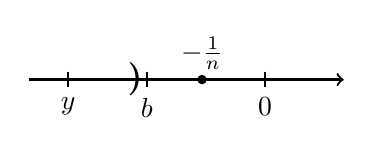
\begin{tikzpicture}[scale=1]
                \draw[thick, ->] (-3,0) -- (1,0);
                \draw[thick] (-2.5,0.1) -- (-2.5,-0.1) node[below] {\(y\)};
                \draw[thick] (-1.5,0.1) -- (-1.5,-0.1) node[below] {\(b\)};
                \node at (-1.65, 0) [scale=1.2] {\textbf{)}};
                \draw[thick] (0,0.1) -- (0,-0.1) node[below] {$0$};
                \filldraw (-0.8,0) circle (1.5pt) node[above] {\(-\frac{1}{n}\)};
            \end{tikzpicture}
            \end{center}
            \(\forall n \ge n_0, \quad b < - \frac{1}{n_0} \le - \frac{1}{n} < 0\). A partir de un \(n_0\) no hay ninguno.
            \[
                \Rightarrow \forall n \ge n_0, \quad -\frac{1}{n} \notin [a, b).
            \]
        \end{itemize}
        No puede ser límite \(\Rightarrow \{-\frac{1}{n}\}_{n \in \mathbb{N}}\) no tiene límite en este espacio topológico.
        
        \item \((\mathbb{R}, \mc T = \{ (-n, n) : n \in \mathbb{N} \} \cup \{ \emptyset, X \})\):
        \[
             \left\{\frac{1}{n}\right\}_{n \in \mathbb{N}} \longrightarrow
            \begin{cases}
                0 & (\text{todos los abiertos contienen al } 0) \\
                \frac{1}{2} & \\
                \lambda \in \mathbb{R} & (\text{converge a cualquier } \lambda \in (-n, n))
            \end{cases}
            \Rightarrow \text{tiene infinitos límites.}
        \]
        \[
            (-n, n) \quad \forall n \in \mathbb{N} \quad \text{y} \quad  \left\{\frac{1}{n}\right\}_{n \ge 1},
        \]
        \[
            (-n, n) \cap  \left\{\frac{1}{n}\right\}_{n \in \mathbb{N}} =  \left\{\frac{1}{n}\right\}_{n \ge 2}.
        \]
    \end{enumerate}
\end{ejems}

\begin{prop}
    Si la sucesión \(\{x_n\}_{n \in \mathbb{N}}\) \textbf{no constante} tiene por límite el punto \(y \in X\), entonces para cualquier subconjunto \(A \subseteq X\) tal que \(\{x_n\}_{n \in \mathbb{N}} \subseteq A\), se verifica que \(y\) es punto de acumulación de \(A\).
\end{prop}

\begin{dem}
    Para todo abierto \(U_y\), veamos que \((U_y \cap A) \setminus \{y\} \ne \emptyset\).
    
    Como \(y\) es límite, \(\exists n_0 \in \mathbb{N}\) tal que \(\forall n \ge n_0\),
    \[
        x_n \in U_y \Rightarrow \underbrace{x_n}_{\in A} \in U_y \cap A \Rightarrow x_n \in U_y \cap A \quad \text{con } x_n \ne y.
    \]
\end{dem}

\begin{obs}
    El recíproco en general es falso.
\end{obs}

\section{Condiciones o axiomas de separaci\'on}
Sea $X$ un espacio topol\'ogico. 
\begin{defi} Se tienen las siguientes definiciones de condiciones de separaci\'on 
    \begin{itemize}
        \item Un espacio topol\'ogico $X$ es \textbf{$T_0$} (o \textbf{de Kolmogorov}) si para cualesquiera puntos distintos $x\neq x' \in X$ existe un abierto $U_x$ con $x\in U_x$ y $x'\nin U_x$ \underline{o} existe un abierto $U_{x'}$ con $x'\in U_{x'}$ y $x\nin U_{x'}$.
        \item Un espacio topol\'ogico $X$ es \textbf{$T_1$} (o \textbf{de Fréchet}) si para cualesquiera puntos distintos $x\neq x' \in X$ existe un abierto $U_x$ con $x\in U_x$ y $x'\nin U_x$ \underline{y} existe un abierto $U_{x'}$ con $x'\in U_{x'}$ y $x\nin U_{x'}$. 
        \item Un espacio topol\'ogico $X$ es \textbf{$T_2$} (o \textbf{separado} o \textbf{de Hausdorff}) si para cualesquiera puntos distintos $x\neq x' \in X$ existe un abierto $U_x$ con $x\in U_x$ y existe un abierto $U_{x'}$ con $x'\in U_{x'}$ tal que $U_x\cap U_{x'} = \emptyset$. 
        \item Un espacio topol\'ogico $X$ es \textbf{regular} si para cualquier punto $x \in X$ y cualquier cerrado $C\subset X$ con $x\nin C$ existen abiertos $U_x$ y $U_C$ con $x\in U_x$ y $C\subset U_C$ tal que $U_x\cap U_{C} = \emptyset$.
        \item Un espacio topol\'ogico $X$ es \textbf{$T_3$} si es regular y $T_1$ (los puntos son cerrados). 
        \item Un espacio topol\'ogico $X$ es \textbf{normal} si para cualesquiera cerrados $C$ y $C'$ con $C\cap C'=\emptyset$ existen abiertos con $C \subset U_C, \, C'\subset U_{C'}$ tal que $U_C \cap U_{C'}=\emptyset$. 
        \item Un espacio topol\'ogico $X$ es \textbf{$T_4$} si es normal y $T_1$.  
    \end{itemize}
\end{defi}
\begin{obs}
    $T_4  \Rightarrow T_3 \Rightarrow T_2 \Rightarrow T_1 \Rightarrow T_0$.

    Regular $\Rightarrow T_2 \, \iff \{x\}$ es cerrado para todo $x\in X$. 
\end{obs}
\begin{prop}
    Un espacio topol\'ogico $X$ es $T_0$ $\iff$ se verifica que para cualesquiera puntos $x,x' \in X$, $x\neq x' \iff \overline{\{x\}} \neq \overline{\{x'\}} $. 
\end{prop}
\begin{dem}
$\Rightarrow) $ Es trivial que $\overline{\{x\}}\neq \overline{\{x'\}} \Rightarrow x\neq x'$. 

Veamos que $x\neq x' \Rightarrow \overline{\{x\}} \neq \overline{\{x'\}}$. Sean $x\neq x'$, como el espacio es $T_0$ 
$$\begin{cases}
\text{existe } U_x \ni x \text{ con } x' \nin U_x \\[-2mm]  \qquad \text{\'o} \\[-2mm]  \text{existe } U_{x'} \text{ con } x \nin U_{x'} 
\end{cases}\Rightarrow \begin{cases}
U_{x} \cap \{x'\} = \emptyset  \\[-2mm] \qquad  \text{\'o} \\[-2mm]  U_{x'} \cap \{x\} = \emptyset 
\end{cases} \Rightarrow \begin{cases}
x \nin \overline{\{x'\}} \ni x'  \\[-2mm] \qquad  \text{\'o} \\[-2mm]  x' \nin \overline{\{x\}} \ni x
\end{cases} \Rightarrow \overline{\{x\}} \neq  \overline{\{x'\}}$$
$\Leftarrow) $ Sea $x\neq x'\in X$, como $\overline{\{x\}} \neq \overline{\{x'\}}$ por hip\'otesis, 
$$\Rightarrow \begin{cases}
    x\nin \overline{\{x'\}} \\[-2mm] \qquad  \text{ \'o } \\[-2mm] x' \nin \overline{\{x\}} 
\end{cases} \Rightarrow \begin{cases}
    \exists \, U_x \text{ con } U_x \cap \{x'\} =\emptyset \iff x'\nin U_x \\[-2mm] 
    \qquad \text{ \'o} \\
    \exists \, U_{x'} \text{ con } U_{x'} \cap \{x\} =\emptyset \iff x \nin U_{x'}
\end{cases}$$

$\Leftarrow)$ Sean $x \ne x' \in X$. Como $\overline{\{x\}} \ne \overline{\{x'\}}$ por hipótesis, $\implies x \notin \overline{\{x'\}}$ o $x' \notin \overline{\{x\}}$.
    \begin{align*}
        \implies & \exists U_x \text{ abierto con } U_x \cap \{x'\} = \emptyset \iff x' \notin U_x \\
        & \exists U_{x'} \text{ abierto con } U_{x'} \cap \{x\} = \emptyset \iff x \notin U_{x'}
    \end{align*}
    $\implies$ Es $T_0$.
\end{dem}
\begin{prop}
    Un espacio topol\'ogico es $T_1 \, \iff $ todos los puntos de $X$ son cerrados (dicho de otra forma, $\mc T_{cof} \subset \mc T_X$). 
\end{prop}
\begin{dem}
$\Leftarrow) $ Sean $x\neq x'$, $U_x = X- \{x'\}$ y $U_{x'} = X - \{x\}$ son abiertos por ser complementarios de cerrados y $x\in U_x$ pero $x'\nin U_x$, y $x'\in U_{x'}$ pero $x\nin U_{x'}$, que es la condici\'on de $T_1$.

$\Rightarrow)$ Sea $x\in X$ veamos que $\{x\}$ es cerrado. Supongamos que no, entonces $\{x\} \neq \overline{\{x\}}$ con $x'\in \overline{\{x\}}$ y $x\neq x'$, si fuera $T_1$ existe un abierto $U_{x'}$ con $x'\in U_{x'}$, $U_{x'}\cap \{x\} \neq \emptyset$ por propiedades del cierre, por lo que $x \in U_{x'}$ y no ser\'ia $T_1$, llegando a contradicci\'on. Por lo que $\{x\}$ es cerrado. 
\end{dem}

% ==========================================
% PÁGINA 1
% ==========================================
 

\begin{prop}
    Un espacio topológico $X$ es $T_1 \iff$ todos los puntos de $X$ son cerrados.
\end{prop}

\begin{dem} $\Leftarrow)$ Sean $x \ne x'$.
        \[
            \text{Consideramos  } \,  
            \begin{aligned}
                U_x &= X \setminus \{x'\} \ni x \\
                U_{x'} &= X \setminus \{x\} \ni x'
            \end{aligned}
            \quad \text{(abiertos)} \implies \text{Es } T_1.
        \]
        \begin{flushright}
            \footnotesize
            $\rightarrow$ Todos los subconjuntos finitos de puntos son cerrados (uniones finitas de cerrados). \\
            $T_1 \iff \mc T_{cof} \subset \mc T_X$.
        \end{flushright}

        $\Rightarrow)$ Sea $x \in X$. Queremos ver que $\{x\}$ es cerrado.
        
        Supongamos que $\{x\}$ no es cerrado $\iff \{x\} \ne \overline{\{x\}} \implies$ existe $x' \in \overline{\{x\}}$ con $x' \ne x$. Por tanto, 
        \[
            \forall \, U_{x'} \text{ abierto con } x' \in U_{x'}, \quad U_{x'} \cap \{x\} \ne \emptyset \implies x \in U_{x'} \implies \bot \quad (\forall \text{ abierto}).
        \]
\end{dem}

\begin{prop}
    $X$ es $T_2 \iff$ dados $x, x' \in X$ con $x \ne x'$, entonces existe un entorno cerrado $V_x$ con $x \in V_x \not\ni x'$ y viceversa, existe un entorno cerrado $V_{x'}$ con $x' \in V_{x'} \not\ni x$.
\end{prop}

\begin{dem} \, 
    
    $\Rightarrow)$ Sean $x \ne x' \in X$. Por ser $X$ $T_2$, existen abiertos $U_x, U_{x'}$ con $U_x \cap U_{x'} = \emptyset \implies U_x \subseteq \underbrace{X \setminus U_{x'}}_{\text{(Cerrado)}}$. Como $X \setminus U_{x'}$ es cerrado, entonces $x \in U_x \subseteq \underbrace{\overline{U}_x}_{V_x} \subseteq X \setminus U_{x'}$, y concluimos.
\end{dem}

\begin{obs}
    Si $V_x$ es entorno cerrado de $x$, entonces existe un abierto $U_x$ con $$x \in U_x \subseteq \underbrace{\overline{U}_x}_{\substack{\text{entorno} \\ \text{cerrado}}} \subseteq \underbrace{V_x}_{\substack{\text{entorno} \\ \text{cerrado}}}$$
\end{obs}

\begin{dem}[Continuación Prop.] \, 

        $\Leftarrow)$ Sean $x \ne x' \in X$. Por hipótesis, existen cerrados $V_x, V_{x'}$ tal que $x \notin V_{x'}, \, x' \notin V_x$. Entonces, existe un abierto $U_x$ tal que $x \in U_x \subseteq V_x$.      
        Sea $U_{x'} = X \setminus V_x$, que es abierto, y $x' \in X \setminus V_x$. Tenemos que $U_x \cap U_{x'} = \emptyset \implies X$ es $T_2$.
\end{dem}

\begin{prop}
    Si $X$ es $T_2$, si una sucesión de puntos $\{x_n\}_{n \in \mathbb{N}} \subseteq X$ tiene límite, este límite es único.
\end{prop}

\begin{dem}
    Supongamos que la sucesión tiene dos límites, $\lim \{x_n\} = x, \, x'$ y que $x \ne x'$. Por ser $T_2$, existen abiertos $U_x, U_{x'}$ tales que $U_x \cap U_{x'} = \emptyset$.
    
% ==========================================
% PÁGINA 2 (pág. 11)
% ==========================================
    \begin{align*}
        \lim \{x_n\} = x \text{ y } x \in U_x &\implies \exists n_0(U_x) \text{ tal que } \forall n \ge n_0, \, x_n \in U_x. \\
        \lim \{x_n\} = x' \text{ y } x' \in U_{x'} &\implies \exists n_0'(U_{x'}) \text{ tal que } \forall n \ge n_0', \, x_n \in U_{x'}.
    \end{align*}
    Sea $N_0 = \max\{n_0, n_0'\}$.
    \[
        \forall n \ge N_0 \implies 
        \begin{cases} 
            \ge n_0 \implies x_n \in U_x \\ 
            \ge n_0' \implies x_n \in U_{x'} 
        \end{cases} 
        \implies x_n \in U_x \cap U_{x'} \ne \emptyset, \quad \forall n \ge N_0 \implies \bot.
    \]
    \end{dem}
\begin{prop}
    $X$ es regular $\iff$ para todo $x \in X$ y todo abierto $U_x$ con $x \in U_x$, existe un entorno (abierto) $V_x$ de $x$ tal que $x \in V_x \subseteq \overline{V}_x \subseteq U_x$.\vspace{-0.3cm}
    \[\vspace{-0.4cm}
        \Updownarrow
    \]
    \begin{center}
        \small Los entornos cerrados de un punto forman base de entornos del punto.
    \end{center}
    Es decir, los entornos cerrados forman base $\iff X$ es regular.
\end{prop}

\begin{dem} $\Rightarrow) $ Sea $x \in X$ y $U_x$ abierto. $x \notin X \setminus U_x \coloneqq C$ cerrado. Por ser $X$ regular, existen abiertos $V_x \ni x, \, V_C \supset C$ tales que $V_x \cap V_C = \emptyset$.    
        Esto implica que $V_x \subseteq X \setminus V_C \subseteq X \setminus C = U_x \implies x \in V_x \subseteq \overline{V}_x \subseteq X \setminus V_C \subseteq U_x$.

        $\Leftarrow)$ Sea $x \in X, \, C \subseteq X$ cerrado con $x \notin C \implies x \in X \setminus C \coloneqq U_x$ abierto.     
        Por hipótesis, existe $V_x$ abierto con $x \in V_x \subseteq \overline{V}_x \subseteq U_x$.
        Luego $x \in V_x$ y $X \setminus U_x \subseteq \underbrace{X \setminus \overline{V}_x}_{V_C \text{ abierto}}$, con $C = X \setminus U_x$, y $V_x \cap V_C = \emptyset$ porque $V_x \subseteq \overline{V}_x \implies X \setminus \overline{V}_x = V_C$.
\end{dem}

\begin{prop}
    $X$ es normal $\iff$ para todo cerrado $C$ y todo abierto $U_C$ con $C \subseteq U_C$, existe un abierto $V_C$ tal que $C \subseteq V_C \subseteq \overline{V}_C \subseteq U_C$.
    
    Entonces, entornos cerrados de un cerrado son base de entornos de cerrados.
\end{prop}

\begin{dem}
    (\textcolor{red}{Ejercicio}).
\end{dem}

\begin{ejem}
    \hfill
    \begin{itemize}
        \item $(X, \mc T_{\text{trivial}})$ no verifica $T_0$, luego no verifica ninguna condición de separación.
        \item $(X, \mc T_{\text{dis}})$ verifica todas.
        \item $(X = \{0, 1\}, \mc T = \{\emptyset, X, \{1\}\})$ es $T_0$ (puedo separar el $1$), pero \textbf{no} $T_1$ (los puntos no son cerrados, el cero sí y el uno no) $\rightarrow \text{Existe } \{1\} \text{ abierto tal que } 1 \in \{1\}, \, 0 \notin \{1\}$.
        \item $(\mathbb{R}^n, \mc T_d)$ es $T_4$ (probar).
    \end{itemize}
\end{ejem}





























































































\begin{comment}
\section{Subespacios topológicos (Topología relativa)}

\begin{defi}
Sea \((X, \mc T_X)\) un espacio topológico y sea \(Y \subseteq X\) un subconjunto. La \textbf{topología inducida} (o relativa) en \(Y\) por \(X\), denotada por \(\mc T_{|Y}\), es:
\[
    \mc T_{|Y} \coloneqq \{U \cap Y \mid U \in \mc T\} \subseteq \mathcal{P}(Y) \text{}.
\]
El par \((Y, \mc T_{|Y})\) se denomina \textbf{subespacio topológico} de \((X, \mc T)\).
\end{defi}

\begin{prop}
\(\mc T_{|Y}\) es una topología en \(Y\).
\end{prop}

\begin{dem}
\begin{enumerate}
    \item[\textbf{1)}] \(\emptyset = \emptyset \cap Y \in \mc T_{|Y}\) (pues \(\emptyset \in \mc T\)) e \(Y = X \cap Y \in \mc T_{|Y}\) (pues \(X \in \mc T\)).
    \item[\textbf{2)}] Sean \(W_1, \ldots, W_n \in \mc T_{|Y}\). Para cada \(k\), existe \(U_k \in \mc T\) tal que \(W_k = U_k \cap Y\). Entonces:
    \[
        W_1 \cap \ldots \cap W_n = (U_1 \cap Y) \cap \ldots \cap (U_n \cap Y) = (U_1 \cap \ldots \cap U_n) \cap Y \text{}.
    \]
    Como \(U_1 \cap \ldots \cap U_n \in \mc T\), se deduce que \(W_1 \cap \ldots \cap W_n \in \mc T_{|Y}\).
    \item[\textbf{3)}] Sea \(\{W_i\}_{i \in I} \subseteq \mc T_{|Y}\). Para cada \(i \in I\), existe \(U_i \in \mc T\) con \(W_i = U_i \cap Y\). Por distributividad:
    \[
        \bigcup_{i \in I} W_i = \bigcup_{i \in I} (U_i \cap Y) = \left(\bigcup_{i \in I} U_i\right) \cap Y \text{}.
    \]
    Como \(\bigcup_{i \in I} U_i \in \mc T\), su intersección con \(Y\) pertenece a \(\mc T_{|Y}\).
\end{enumerate}
\end{dem}

\begin{obs}
\begin{itemize}
    \item Un abierto \(W \in \mc T_{|Y}\) no tiene por qué ser abierto en \((X, \mc T)\).
    \item Si \(Y \in \mc T\) (es decir, \(Y\) es un subconjunto abierto de \(X\)), entonces todo abierto relativo de \(Y\) es abierto en \(X\), y \(\mc T_{|Y} \subseteq \mc T\).
\end{itemize}
\end{obs}

\begin{ejem}
En \((\mathbb{R}, \mc T_d)\), consideremos \(Y = [1, 2) \cup \{3\} \subset \mathbb{R}\):
\begin{itemize}
    \item \([1, 2) = (0, 2) \cap Y\), con \((0, 2) \in \mc T_d\). Por tanto, \([1, 2)\) es abierto en \((Y, \mc T_{|Y})\), aunque no es abierto en \((\mathbb{R}, \mc T_d)\).
    \item \(\{3\} = (2, 4) \cap Y\), con \((2, 4) \in \mc T_d\). Por tanto, \(\{3\}\) es un abierto en \((Y, \mc T_{|Y})\).
\end{itemize}
\end{ejem}

\section{Topología por entornos}


\begin{teo}
Sea \(X\) un conjunto y sea \(\{\mathcal{E}'(x)\}_{x \in X}\) una familia de subconjuntos de \(X\) asignada a cada punto \(x \in X\) que satisface los axiomas 1, 2, 3 y 4 anteriores. Entonces existe una \textbf{única} topología \(\mc T'\) en \(X\) tal que \(\mathcal{E}_{\mc T'}(x) = \mathcal{E}'(x)\) para todo \(x \in X\).
\end{teo}

\begin{dem}
Definimos la familia:
\[
    \mc T' \coloneqq \{U \subseteq X \mid \forall x \in U, \; U \in \mathcal{E}'(x)\} \text{}.
\]
\begin{itemize}
    \item[\textbf{a)}] \(\mc T'\) es topología:
    \begin{itemize}
        \item \(\emptyset \in \mc T'\) por vacuidad. Para todo \(x \in X\), por el axioma 1 tenemos \(x \in V\) para cualquier \(V \in \mathcal{E}'(x)\), y como \(V \subseteq X\), por el axioma 3 se tiene \(X \in \mathcal{E}'(x)\), luego \(X \in \mc T'\).
        \item Si \(U_1, U_2 \in \mc T'\) y \(x \in U_1 \cap U_2\), entonces \(U_1 \in \mathcal{E}'(x)\) y \(U_2 \in \mathcal{E}'(x)\). Por el axioma 2, \(U_1 \cap U_2 \in \mathcal{E}'(x)\), luego \(U_1 \cap U_2 \in \mc T'\).
        \item Si \(\{U_i\}_{i \in I} \subseteq \mc T'\) y \(x \in \bigcup_{i \in I} U_i\), existe \(j \in I\) con \(x \in U_j\), luego \(U_j \in \mathcal{E}'(x)\). Al ser \(U_j \subseteq \bigcup U_i\), por el axioma 3 se tiene \(\bigcup U_i \in \mathcal{E}'(x)\), luego \(\bigcup U_i \in \mc T'\).
    \end{itemize}
    \item[\textbf{b)}] Coincidencia de entornos:
    \begin{itemize}
        \item Si \(V \in \mathcal{E}_{\mc T'}(x)\), existe \(U \in \mc T'\) con \(x \in U \subseteq V\). Por definición de \(\mc T'\), \(U \in \mathcal{E}'(x)\), y por el axioma 3, \(V \in \mathcal{E}'(x)\).
        \item Si \(V' \in \mathcal{E}'(x)\), definimos \(U \coloneqq \{y \in X \mid V' \in \mathcal{E}'(y)\}\). Por el axioma 1, \(y \in U \Rightarrow y \in V'\), luego \(U \subseteq V'\). Veamos que \(U \in \mc T'\): si \(y \in U\), entonces \(V' \in \mathcal{E}'(y)\); por el axioma 4, existe \(W \in \mathcal{E}'(y)\) tal que para todo \(z \in W\) se cumple \(V' \in \mathcal{E}'(z)\) (lo que significa \(W \subseteq U\)), luego por el axioma 3, \(U \in \mathcal{E}'(y)\). Por tanto, \(U \in \mc T'\). Como \(x \in U \subseteq V'\), deducimos que \(V' \in \mathcal{E}_{\mc T'}(x)\).
    \end{itemize}
    \item[\textbf{c)}] Unicidad: si \(\mc T''\) tuviera los mismos entornos, un subconjunto sería abierto si y solo si es entorno de todos sus puntos, lo que forzaría \(\mc T'' = \mc T'\).
\end{itemize}
\end{dem}

\subsection{Bases de entornos (Sistemas fundamentales de entornos)}

\begin{defi}
Sea \((X, \mc T)\) un espacio topológico y \(x \in X\). Una subfamilia \(\mathcal{B}(x) \subseteq \mathcal{E}(x)\) es una \textbf{base de entornos} de \(x\) si para todo entorno \(V \in \mathcal{E}(x)\) existe \(B_x \in \mathcal{B}(x)\) tal que:
\[
    x \in B_x \subseteq V \text{}.
\]
\end{defi}

\begin{prop}
Si \(\{\mathcal{B}(x)\}_{x \in X}\) es una base de entornos para cada \(x \in X\), entonces verifica:
\begin{enumerate}
    \item[\textbf{1)}] \(\forall B \in \mathcal{B}(x)\), \(x \in B\).
    \item[\textbf{2)}] \(\forall B_1, B_2 \in \mathcal{B}(x)\), existe \(B_0 \in \mathcal{B}(x)\) tal que \(B_0 \subseteq B_1 \cap B_2\).
    \item[\textbf{3)}] \(\forall B \in \mathcal{B}(x)\), existe \(B_x \in \mathcal{B}(x)\) tal que para todo \(y \in B_x\) existe \(B_y \in \mathcal{B}(y)\) con \(B_y \subseteq B\).
\end{enumerate}
\end{prop}

\begin{dem}
\begin{enumerate}
    \item[\textbf{1)}] Como \(\mathcal{B}(x) \subseteq \mathcal{E}(x)\), todo \(B \in \mathcal{B}(x)\) es entorno de \(x\), luego \(x \in B\).
    \item[\textbf{2)}] Sean \(B_1, B_2 \in \mathcal{B}(x) \subseteq \mathcal{E}(x)\). Su intersección \(B_1 \cap B_2 \in \mathcal{E}(x)\). Como \(\mathcal{B}(x)\) es base de entornos, existe \(B_0 \in \mathcal{B}(x)\) con \(B_0 \subseteq B_1 \cap B_2\).
    \item[\textbf{3)}] Sea \(B \in \mathcal{B}(x) \subseteq \mathcal{E}(x)\). Por el axioma 4 de entornos, existe \(W \in \mathcal{E}(x)\) tal que para todo \(y \in W\) se tiene \(B \in \mathcal{E}(y)\). Como \(\mathcal{B}(x)\) es base de entornos, existe \(B_x \in \mathcal{B}(x)\) con \(B_x \subseteq W\). Entonces para todo \(y \in B_x \subseteq W\), se cumple \(B \in \mathcal{E}(y)\); como \(\mathcal{B}(y)\) es base de entornos, existe \(B_y \in \mathcal{B}(y)\) tal que \(B_y \subseteq B\).
\end{enumerate}
\end{dem}

\begin{teo}
Dada una familia \(\{\mathcal{B}(x)\}_{x \in X}\) de subconjuntos de \(X\) que satisface las tres propiedades anteriores, existe una única topología en \(X\) de la cual \(\{\mathcal{B}(x)\}\) son bases de entornos.
\end{teo}

\begin{dem}
Definimos para cada \(x \in X\):
\[
    \mathcal{E}(x) \coloneqq \{V \subseteq X \mid \exists B_x \in \mathcal{B}(x) \text{ tal que } x \in B_x \subseteq V\} \text{}.
\]
Comprobamos que \(\mathcal{E}(x)\) verifica los 4 axiomas del Teorema 5.2:
\begin{enumerate}
    \item[\textbf{1)}] Si \(V \in \mathcal{E}(x)\), existe \(B_x \in \mathcal{B}(x)\) con \(x \in B_x \subseteq V\). Por la propiedad 1, \(x \in B_x\), luego \(x \in V\).
    \item[\textbf{2)}] Si \(V_1, V_2 \in \mathcal{E}(x)\), existen \(B_1, B_2 \in \mathcal{B}(x)\) con \(B_1 \subseteq V_1\) y \(B_2 \subseteq V_2\). Por la propiedad 2, existe \(B_0 \in \mathcal{B}(x)\) con \(B_0 \subseteq B_1 \cap B_2 \subseteq V_1 \cap V_2\), luego \(V_1 \cap V_2 \in \mathcal{E}(x)\).
    \item[\textbf{3)}] Si \(V \in \mathcal{E}(x)\) y \(V \subseteq W\), existe \(B_x \in \mathcal{B}(x)\) con \(B_x \subseteq V \subseteq W\), luego \(W \in \mathcal{E}(x)\).
    \item[\textbf{4)}] Si \(V \in \mathcal{E}(x)\), existe \(B \in \mathcal{B}(x)\) con \(B \subseteq V\). Por la propiedad 3, existe \(B_x \in \mathcal{B}(x)\) tal que para todo \(y \in B_x\) existe \(B_y \in \mathcal{B}(y)\) con \(B_y \subseteq B \subseteq V\). Tomamos \(W \coloneqq B_x \in \mathcal{B}(x) \subseteq \mathcal{E}(x)\). Para todo \(y \in W\), como \(B_y \subseteq V\), se sigue que \(V \in \mathcal{E}(y)\).
\end{enumerate}
Por el Teorema 5.2, existe una única topología inducida que tiene a \(\mathcal{E}(x)\) como entornos y a \(\mathcal{B}(x)\) como bases de entornos.
\end{dem}

\begin{ejem}
En \((\mathbb{R}^n, d)\) con la distancia euclídea usual:
\begin{itemize}
    \item \(\mathcal{B}(x) = \{B_d(x, \varepsilon) \mid \varepsilon > 0\}\) es una base de entornos de \(x\).
    \item \(\mathcal{B}'(x) = \{B_d(x, \nicefrac{1}{n}) \mid n \in \mathbb{N}\}\) es una base numerable de entornos de \(x\).
    \item \(\overline{\mathcal{B}}(x) = \{\overline{B_d}(x, \nicefrac{1}{n}) \mid n \in \mathbb{N}\}\) (bolas cerradas) también forma una base de entornos, puesto que \(\overline{B_d}(x, \nicefrac{1}{2n}) \subseteq B_d(x, \nicefrac{1}{n})\).
\end{itemize}
\end{ejem}











\chapter{Elementos de un espacio topológico}
Sea $X$ un espacio topológico e $Y \subseteq X$ un subconjunto.

\section{Interior, cierre y puntos especiales}


\begin{defi}
El conjunto de los \textbf{puntos de acumulación} de $Y$ (o conjunto derivado), denotado por $Y'$, es:
\[
    Y' \coloneqq \{x \in X \mid \forall U_x \text{ abierto con } x \in U_x, \; (U_x \setminus \{x\}) \cap Y \ne \emptyset\}.
\]
Se verifica que:
\[
    \overline{Y} = Y \cup Y'.
\]
\end{defi}

\begin{dem}
Sea $x \in \overline{Y}$. Para todo entorno abierto $U_x \ni x$, $U_x \cap Y \ne \emptyset$. Pueden darse dos casos:
\begin{enumerate}
    \item Existe algún $U_x$ tal que $U_x \cap Y = \{x\}$, lo cual implica $x \in Y \subseteq Y \cup Y'$.
    \item Para todo $U_x$, $U_x \cap Y \ne \{x\}$, lo cual equivale a $(U_x \setminus \{x\}) \cap Y \ne \emptyset$, luego $x \in Y' \subseteq Y \cup Y'$.
\end{enumerate}
Recíprocamente, como $Y \subseteq \overline{Y}$ e $Y' \subseteq \overline{Y}$, se tiene $Y \cup Y' \subseteq \overline{Y}$.
\end{dem}

\begin{defi}
Los \textbf{puntos aislados} de $Y$ son aquellos puntos de $Y$ que no son de acumulación:
\[
    Y^a \coloneqq \{y \in Y \mid \exists U_y \subseteq X \text{ abierto con } y \in U_y \text{ tal que } U_y \cap Y = \{y\}\}.
\]
Equivalentemente, $Y^a = \{y \in Y \mid \{y\} \text{ es abierto en } (Y, \mc T_{|Y})\}$. Se verifica que $\overline{Y} = Y^a \sqcup Y'$.
\end{defi}

\begin{ejem}
En $\mathbb{R}^2$ con la topología usual, sea $Y = [1, 3) \times [1, 2) \cup \{(4, 1), (5, 1)\}$:
\begin{itemize}
    \item $Y^\circ = (1, 3) \times (1, 2)$.
    \item $\overline{Y} = [1, 3] \times [1, 2] \cup \{(4, 1), (5, 1)\}$.
    \item $Y' = [1, 3] \times [1, 2]$.
    \item $Y^a = \{(4, 1), (5, 1)\}$.
\end{itemize}
\end{ejem}

\begin{defi}
La \textbf{frontera} de $Y$ se define como:
\[
    \operatorname{Fr}(Y) = \partial(Y) \coloneqq \overline{Y} \cap \overline{X \setminus Y} = \operatorname{Fr}(X \setminus Y).
\]
\end{defi}

\begin{defi}
El \textbf{borde} de $Y$ es:
\[
    b(Y) \coloneqq Y \cap \operatorname{Fr}(Y) = Y \cap (\overline{Y} \cap \overline{X \setminus Y}) = Y \cap \overline{X \setminus Y}.
\]
\end{defi}

\begin{defi}
El \textbf{exterior} de $Y$ es el interior de su complementario:
\[
    \operatorname{Ext}(Y) \coloneqq (X \setminus Y)^\circ.
\]
\end{defi}

\begin{ejem}
En $(\mathbb{R}, \mc T_d)$, sea $Y = [0, 1)$:
\begin{itemize}
    \item $Y^\circ = (0, 1)$, $\overline{Y} = [0, 1]$, $Y' = [0, 1]$, $Y^a = \emptyset$.
    \item $X \setminus Y = (-\infty, 0) \cup [1, \infty)$, $\overline{X \setminus Y} = (-\infty, 0] \cup [1, \infty)$.
    \item $\operatorname{Fr}(Y) = \{0, 1\}$.
    \item $b(Y) = \{0\}$.
    \item $\operatorname{Ext}(Y) = (-\infty, 0) \cup (1, \infty)$.
\end{itemize}
\end{ejem}

\section{Propiedades fundamentales de los operadores}

\begin{propi}
Sean $X$ un espacio topológico e $Y \subseteq X$. Se verifican:
\begin{enumerate}
    \item[\textbf{I.}] $Y^\circ \cap \operatorname{Fr}(Y) = \emptyset$.
    \item[\textbf{II.}] $\operatorname{Ext}(Y) \cap \operatorname{Fr}(Y) = \emptyset$.
    \item[\textbf{III.}] $Y^\circ \cap b(Y) = \emptyset$.
    \item[\textbf{IV.}] $Y = Y^\circ \sqcup b(Y)$.
    \item[\textbf{V.}] $\overline{Y} = Y^\circ \sqcup \operatorname{Fr}(Y)$.
    \item[\textbf{VI.}] $Y$ es abierto $\iff b(Y) = \emptyset$.
    \item[\textbf{VII.}] $Y$ es cerrado $\iff \operatorname{Fr}(Y) \subseteq Y$.
    \item[\textbf{VIII.}] $\operatorname{Ext}(Y) = X \setminus \overline{Y}$.
    \item[\textbf{IX.}] $\overline{X \setminus Y} = X \setminus Y^\circ$.
    \item[\textbf{X.}] $\overline{Y^\circ} \subseteq \overline{Y}$ (en general no se da la igualdad).
    \item[\textbf{XI.}] $Y^\circ \subseteq (\overline{Y})^\circ$ (en general no se da la igualdad).
\end{enumerate}
\end{propi}

\begin{dem}
\begin{itemize}
    \item[\textbf{I.}] $Y^\circ \cap \operatorname{Fr}(Y) = Y^\circ \cap (\overline{Y} \cap \overline{X \setminus Y}) = Y^\circ \cap \overline{X \setminus Y} = \emptyset$, pues si $y \in Y^\circ$, existe un abierto $U_y \subseteq Y$, con lo cual $U_y \cap (X \setminus Y) = \emptyset$, lo que implica $y \notin \overline{X \setminus Y}$.
    \item[\textbf{II.}] $\operatorname{Ext}(Y) \cap \operatorname{Fr}(Y) = (X \setminus Y)^\circ \cap \operatorname{Fr}(X \setminus Y) = \emptyset$ aplicando la propiedad I a $X \setminus Y$.
    \item[\textbf{III.}] $Y^\circ \cap b(Y) = Y^\circ \cap (Y \cap \operatorname{Fr}(Y)) = Y^\circ \cap \operatorname{Fr}(Y) = \emptyset$.
    \item[\textbf{IV.}] Si $y \in Y$, o bien $y \in Y^\circ$, o bien para todo abierto $U \ni y$ se tiene $U \not\subseteq Y$, es decir, $U \cap (X \setminus Y) \ne \emptyset$, lo que implica $y \in \overline{X \setminus Y}$; luego $y \in Y \cap \overline{X \setminus Y} = b(Y)$. La unión es disjunta por III.
    \item[\textbf{V.}] Análoga a IV usando $\overline{Y}$ y $\operatorname{Fr}(Y)$.
    \item[\textbf{VI.}] $Y$ es abierto $\iff Y = Y^\circ \iff b(Y) = Y \setminus Y^\circ = \emptyset$.
    \item[\textbf{VII.}] $Y$ es cerrado $\iff X \setminus Y$ es abierto $\iff b(X \setminus Y) = \emptyset \iff (X \setminus Y) \cap \operatorname{Fr}(Y) = \emptyset \iff \operatorname{Fr}(Y) \subseteq Y$.
    \item[\textbf{VIII.}] $x \in \operatorname{Ext}(Y) \iff x \in (X \setminus Y)^\circ \iff \exists U_x \text{ abierto con } U_x \subseteq X \setminus Y \iff U_x \cap Y = \emptyset \iff x \notin \overline{Y} \iff x \in X \setminus \overline{Y}$.
    \item[\textbf{IX.}] Tomando complementarios en VIII: $\overline{X \setminus Y} = X \setminus (X \setminus (X \setminus Y))^\circ = X \setminus Y^\circ$.
    \item[\textbf{X.}] Como $Y^\circ \subseteq Y \Rightarrow \overline{Y^\circ} \subseteq \overline{Y}$. En $(\mathbb{R}, \mc T_d)$, para $\mathbb{Q}$ se tiene $\mathbb{Q}^\circ = \emptyset \Rightarrow \overline{\mathbb{Q}^\circ} = \emptyset \ne \mathbb{R} = \overline{\mathbb{Q}}$.
    \item[\textbf{XI.}] Como $Y^\circ$ es un abierto contenido en $Y \subseteq \overline{Y}$, necesariamente $Y^\circ \subseteq (\overline{Y})^\circ$. Para $\mathbb{Q}$ en $\mathbb{R}$: $\mathbb{Q}^\circ = \emptyset$, pero $(\overline{\mathbb{Q}})^\circ = \mathbb{R}^\circ = \mathbb{R}$.
\end{itemize}
\end{dem}

\section{Subconjuntos densos y clausura relativa}

\begin{defi}
Sea $X$ un espacio topológico e $Y \subseteq X$. Se dice que $Y$ es \textbf{denso} en $X$ si su cierre es el espacio total:
\[
    \overline{Y} = X.
\]
\end{defi}

\begin{prop}
Un subconjunto $Y \subseteq X$ es denso $\iff$ todo abierto no vacío $U \subseteq X$ corta a $Y$ ($U \cap Y \ne \emptyset$).
\end{prop}

\begin{dem}
($\Rightarrow$) Sea $U \ne \emptyset$ abierto en $X$. Sea $x \in U$. Como $X = \overline{Y}$, $x \in \overline{Y}$, por lo que todo entorno abierto de $x$ corta a $Y$; en particular, $U \cap Y \ne \emptyset$.

($\Leftarrow$) Sea $x \in X$. Todo abierto $U \ni x$ es no vacío, luego corta a $Y$, de donde $x \in \overline{Y}$. Por tanto, $X \subseteq \overline{Y} \Rightarrow \overline{Y} = X$.
\end{dem}

\begin{prop}
Sea $Y \subseteq X$ un subespacio topológico y sea $Z \subseteq Y$. Denotemos por $\overline{Z}^X$ la clausura de $Z$ en $X$. Entonces $Z$ es cerrado en $Y$ si y solo si:
\[
    Z = \overline{Z}^X \cap Y.
\]
\end{prop}

\begin{dem}
Si $Z$ es cerrado en $Y$, existe un cerrado $C \subseteq X$ tal que $Z = C \cap Y$. Como $Z \subseteq C$ y $C$ es cerrado en $X$, $\overline{Z}^X \subseteq C$. Por ende, $Z \subseteq \overline{Z}^X \cap Y \subseteq C \cap Y = Z$, de modo que $Z = \overline{Z}^X \cap Y$. El recíproco es inmediato, ya que $\overline{Z}^X$ es cerrado en $X$.
\end{dem}






























\section{Límites de sucesiones}

\begin{defi}
Sea $X$ un espacio topológico y $\{x_n\}_{n \in \mathbb{N}} \subseteq X$ una sucesión de puntos en $X$ (es decir, una aplicación $x \colon \mathbb{N} \to X$). Se dice que un punto $y \in X$ es \textbf{límite} de la sucesión $\{x_n\}$ (y escribimos $\lim_{n \to \infty} x_n = y$) si para todo entorno $V \in \mathcal{E}(y)$ (o para todo abierto $U \ni y$), existe $n_0(V) \in \mathbb{N}$ tal que:
\[
    \forall n \ge n_0(V), \quad x_n \in V.
\]
\end{defi}

\begin{defi}
Una sucesión $\{x_n\}$ es \textbf{no constante} si para todo $n_0 \in \mathbb{N}$ existe $n > n_0$ tal que $x_n \ne x_{n_0}$. Si una sucesión es constante a partir de un término, existe $n_0$ tal que $\forall n \ge n_0$, $x_n = x_{n_0}$, en cuyo caso $\lim x_n = x_{n_0}$.
\end{defi}

\begin{propi}
Sea $\{x_n\} \subseteq X$ una sucesión no constante tal que $\lim_{n \to \infty} x_n = y$. Si consideramos el conjunto de sus términos $S = \{x_n\}_{n \in \mathbb{N}} \subseteq X$, entonces $y \in S'$. En particular, si $S \subseteq A$, entonces $y \in A'$.
\end{propi}

\begin{dem}
Basta probar que para todo entorno $V \in \mathcal{E}(y)$, $(V \setminus \{y\}) \cap S \ne \emptyset$. Como $\lim x_n = y$, existe $n_0$ tal que $\forall n \ge n_0$, $x_n \in V$. Al ser $\{x_n\}$ no constante, existen términos con $x_n \ne y$, luego $(V \setminus \{y\}) \cap S \ne \emptyset$, concluyendo que $y \in S'$.
\end{dem}

\begin{obs}
El recíproco no es cierto en general (en espacios métricos $(\mathbb{R}^n, \mc T_d)$ sí lo es). Además, en un espacio topológico general, el límite de una sucesión \textbf{no tiene por qué ser único}.
\end{obs}

\begin{ejem}
\begin{itemize}
    \item En $(\mathbb{R}, \mc T = \{\emptyset, \mathbb{R}\} \cup \{(-n, n) \mid n \in \mathbb{N}\})$, consideremos $\{\nicefrac{1}{n}\}$. Se tiene que $\lim_{n \to \infty} \nicefrac{1}{n} = a$ para \textbf{todo} $a \in \mathbb{R}$, ya que dado cualquier abierto no vacío $(-m, m)$, existe $n_0$ a partir del cual $\nicefrac{1}{n} \in (-m, m)$ y todo punto $a$ está en algún $(-m, m)$.
    \item En la recta de Sorgenfrey $(\mathbb{R}, \mc T_{\text{Sorg}})$: para la sucesión $\{-\nicefrac{1}{n}\}$, se tiene que $\lim_{n \to \infty} (-\nicefrac{1}{n})$ no converge a $0$, pues $[0, 1) \cap \{-\nicefrac{1}{n}\} = \emptyset$. En cambio, $\{\nicefrac{1}{n}\}$ sí converge únicamente a $0$.
\end{itemize}
\end{ejem}

\section{Axiomas de separación}

Sea $X$ un espacio topológico:
\begin{itemize}
    \item \textbf{Axioma $T_0$ (de Kolmogorov):} Para cualesquiera $x \ne x' \in X$, existe un abierto $U_x$ con $x \in U_x$ y $x' \notin U_x$, o bien existe un abierto $U_{x'}$ con $x' \in U_{x'}$ y $x \notin U_{x'}$.
    \item \textbf{Axioma $T_1$ (de Fréchet):} Para cualesquiera $x \ne x' \in X$, existe un abierto $U_x$ con $x \in U_x$, $x' \notin U_x$, y existe un abierto $U_{x'}$ con $x' \in U_{x'}$, $x \notin U_{x'}$.
    \item \textbf{Axioma $T_2$ (de Hausdorff o separado):} Para cualesquiera $x \ne x' \in X$, existen abiertos disjuntos $U_x, U_{x'}$ con $x \in U_x$, $x' \in U_{x'}$ y $U_x \cap U_{x'} = \emptyset$.
    \item \textbf{Axioma $T_3$ (regular):} $X$ es $T_1$ y para todo punto $x \in X$ y todo cerrado $C \subseteq X$ con $x \notin C$, existen abiertos disjuntos $U_x, U_C$ tales que $x \in U_x$, $C \subseteq U_C$ y $U_x \cap U_C = \emptyset$.
    \item \textbf{Axioma $T_{3\,1/2}$ (de Tychonoff o completamente regular):} $X$ es $T_1$ y para todo $x \in X$ y todo cerrado $C \subseteq X$ con $x \notin C$, existe una función continua $f \colon X \to [0, 1]$ tal que $f(x) = 0$ y $f(C) = \{1\}$.
    \item \textbf{Axioma $T_4$ (normal):} $X$ es $T_1$ y para cualesquiera cerrados disjuntos $C_1, C_2 \subseteq X$ ($C_1 \cap C_2 = \emptyset$), existen abiertos disjuntos $U_{C_1}, U_{C_2}$ con $C_1 \subseteq U_{C_1}$, $C_2 \subseteq U_{C_2}$ y $U_{C_1} \cap U_{C_2} = \emptyset$.
\end{itemize}

\begin{obs}
Se verifican las implicaciones:
\[
    T_4 \Rightarrow T_{3\,1/2} \Rightarrow T_3 \Rightarrow T_2 \Rightarrow T_1 \Rightarrow T_0.
\]
En un espacio $T_2$, si una sucesión converge, su límite es \textbf{único}.
\end{obs}

\begin{ejem}
\begin{itemize}
    \item $(X, \mc T_{\text{trivial}})$ con $|X| \ge 2$ no verifica ningún axioma de separación.
    \item El espacio de Sierpiński $X = \{a, b\}$ con $\mc T = \{\emptyset, X, \{a\}\}$ es $T_0$, pero no es $T_1$.
    \item $(\mathbb{R}^n, \mc T_d)$ es un espacio $T_4$ (y por tanto cumple todos los axiomas anteriores).
\end{itemize}
\end{ejem}

\subsection*{Caracterizaciones de los axiomas de separación}

\begin{prop}
Un espacio topológico $X$ es $T_0 \iff$ puntos distintos tienen clausuras distintas, es decir:
\[
    x \ne y \Rightarrow \overline{\{x\}} \ne \overline{\{y\}}.
\]
\end{prop}

\begin{dem}
($\Rightarrow$) Supongamos que $\overline{\{x\}} = \overline{\{y\}}$. Como $x \in \overline{\{x\}} = \overline{\{y\}}$, todo abierto que contiene a $x$ corta a $\{y\}$, es decir, contiene a $y$. Análogamente, todo abierto que contiene a $y$ contiene a $x$. Por tanto, no puede existir un abierto que contenga a uno sin contener al otro, contradiciendo que $X$ es $T_0$.

($\Leftarrow$) Si $x \ne y$ y $\overline{\{x\}} \ne \overline{\{y\}}$, existe sin pérdida de generalidad un punto $z \in \overline{\{x\}} \setminus \overline{\{y\}}$. Como $z \notin \overline{\{y\}}$, existe un abierto $U$ con $z \in U$ tal que $U \cap \{y\} = \emptyset$, luego $y \notin U$. Como $z \in \overline{\{x\}}$, $U \cap \{x\} \ne \emptyset \Rightarrow x \in U$. Así, $U$ contiene a $x$ pero no a $y$, concluyendo que $X$ es $T_0$.
\end{dem}

\begin{prop}
Un espacio topológico $X$ es $T_1 \iff$ todos los conjuntos unitarios $\{x\}$ son cerrados ($\overline{\{x\}} = \{x\}$ para todo $x \in X$).
\end{prop}

\begin{dem}
($\Rightarrow$) Para todo $y \ne x$, por ser $T_1$ existe un abierto $U_y$ con $y \in U_y$ y $x \notin U_y$. Entonces $X \setminus \{x\} = \bigcup_{y \ne x} U_y$ es unión de abiertos, luego es abierto, y $\{x\}$ es cerrado.

($\Leftarrow$) Si los puntos son cerrados, para $x \ne y$, $U_x = X \setminus \{y\}$ es un abierto con $x \in U_x$, $y \notin U_x$, y $U_y = X \setminus \{x\}$ es un abierto con $y \in U_y$, $x \notin U_y$. Por tanto, $X$ es $T_1$.
\end{dem}

\begin{prop}
Un espacio topológico $X$ es $T_2 \iff$ para cualesquiera $x \ne y \in X$, existen abiertos $U_x, U_y$ tales que:
\[
    \overline{U}_x \cap U_y = \emptyset.
\]
\end{prop}

\begin{dem}
($\Rightarrow$) Si $X$ es $T_2$, existen abiertos disjuntos $U_x, V$ con $x \in U_x$, $y \in V$. Como $U_x \subseteq X \setminus V$ y $X \setminus V$ es cerrado, $\overline{U}_x \subseteq X \setminus V$, de donde $\overline{U}_x \cap V = \emptyset$. Tomando $U_y = V$ se tiene el resultado.

($\Leftarrow$) Si $\overline{U}_x \cap U_y = \emptyset$, como $U_x \subseteq \overline{U}_x$, se deduce $U_x \cap U_y = \emptyset$, luego $X$ es $T_2$.
\end{dem}

\begin{prop}
Un espacio $T_1$ es $T_3 \iff$ para todo punto $x \in X$ y todo abierto $U \ni x$, existe un abierto $V$ tal que:
\[
    x \in V \subseteq \overline{V} \subseteq U.
\]
\end{prop}

\begin{dem}
($\Rightarrow$) Sea $x \in U$ abierto. El conjunto $C = X \setminus U$ es cerrado y $x \notin C$. Por ser $T_3$, existen abiertos disjuntos $V_x, V_C$ con $x \in V_x$ y $C \subseteq V_C$. Como $V_x \cap V_C = \emptyset$, $V_x \subseteq X \setminus V_C \Rightarrow \overline{V}_x \subseteq X \setminus V_C \subseteq X \setminus C = U$.

($\Leftarrow$) Sea $C$ cerrado y $x \notin C$. Entonces $U = X \setminus C$ es un abierto que contiene a $x$. Por hipótesis, existe un abierto $V_1$ con $x \in V_1 \subseteq \overline{V}_1 \subseteq U$. Tomando $V_2 = X \setminus \overline{V}_1$, $V_2$ es abierto, $C = X \setminus U \subseteq V_2$ y $V_1 \cap V_2 = \emptyset$. Luego $X$ es $T_3$.
\end{dem}

\begin{obs}
La proposición anterior equivale a afirmar que en un espacio regular, los entornos cerrados de cada punto forman una base de entornos de dicho punto.
\end{obs}

\begin{prop}
Un espacio $T_1$ es $T_4 \iff$ para todo cerrado $C \subseteq X$ y todo abierto $U$ con $C \subseteq U$, existe un abierto $V$ tal que:
\[
    C \subseteq V \subseteq \overline{V} \subseteq U.
\]
\end{prop}

\begin{dem}
($\Rightarrow$) Si $C \subseteq U$, $C' = X \setminus U$ es cerrado y disjunto con $C$. Por ser $T_4$, existen abiertos disjuntos $V, V'$ con $C \subseteq V$ y $C' \subseteq V'$. Entonces $\overline{V} \subseteq X \setminus V' \subseteq X \setminus C' = U$.

($\Leftarrow$) Si $C_1 \cap C_2 = \emptyset$, $C_1 \subseteq X \setminus C_2 = U$ abierto. Existe un abierto $V$ con $C_1 \subseteq V \subseteq \overline{V} \subseteq U$. Tomando $V_2 = X \setminus \overline{V}$, $V$ y $V_2$ son abiertos disjuntos que separan $C_1$ y $C_2$.
\end{dem}

\begin{defi}
Sea $X$ un espacio topológico y $A \subseteq X$. Un subconjunto $W \subseteq X$ es un \textbf{entorno de $A$} si existe un abierto $V \subseteq X$ tal que $A \subseteq V \subseteq W$.
\end{defi}

\begin{obs}
De forma análoga al caso de puntos, la caracterización de $T_4$ equivale a que los entornos cerrados de un conjunto cerrado forman una base de entornos de dicho cerrado.
\end{obs}

\begin{obs}
En un espacio topológico $X$, todo punto $x \in X$ es un conjunto abierto $\iff X$ tiene la topología discreta.
\end{obs}

























\chapter{Aplicaciones continuas}

\section{Definición de aplicación continua}

\begin{defi}
Sean $(X, \mc T_X)$ e $(Y, \mc T_Y)$ espacios topológicos. Una aplicación $f \colon (X, \mc T_X) \to (Y, \mc T_Y)$ se dice \textbf{continua} si:
\[
    f^*(\mc T_Y) \subseteq \mc T_X.
\]
Es decir, para todo abierto $V \in \mc T_Y$, su anti-imagen es abierta en $X$:
\[
    f^{-1}(V) \in \mc T_X.
\]
Son condiciones equivalentes:
\begin{enumerate}
    \item[\textbf{1)}] $f$ es continua.
    \item[\textbf{2)}] Para todo cerrado $Z \subseteq Y$, su anti-imagen $f^{-1}(Z) \subseteq X$ es un conjunto cerrado en $X$.
    \item[\textbf{3)}] Para todo punto $x \in X$ y para todo entorno $W \in \mathcal{E}(f(x))$, $f^{-1}(W)$ es un entorno de $x$ en $X$ ($f^{-1}(W) \in \mathcal{E}(x)$).
\end{enumerate}
\end{defi}

\begin{prop}
Sea $\mathcal{B}$ una base de la topología $\mc T_Y$ de $Y$. Son equivalentes:
\begin{enumerate}
    \item[\textbf{1)}] $f$ es continua.
    \item[\textbf{2)}] Para todo abierto básico $B \in \mathcal{B}$, $f^{-1}(B)$ es abierto en $X$.
    \item[\textbf{3)}] Para todo cerrado básico $B \in \mathcal{B}_{\text{cerr}}$, $f^{-1}(B)$ es cerrado en $X$.
    \item[\textbf{4)}] Para todo $x \in X$ y todo entorno básico $B \in \mathcal{B}(f(x))$, $f^{-1}(B)$ es entorno de $x$.
\end{enumerate}
\end{prop}

\begin{dem}
\begin{itemize}
    \item[\textbf{1 $\Rightarrow$ 2:}] Inmediato, pues todo abierto básico es un abierto de $Y$.
    \item[\textbf{2 $\Rightarrow$ 1:}] Dado $V \in \mc T_Y$, existe una familia $\{B_i\}_{i \in I} \subseteq \mathcal{B}$ tal que $V = \bigcup_{i \in I} B_i$. Entonces:
    \[
        f^{-1}(V) = f^{-1}\left(\bigcup_{i \in I} B_i\right) = \bigcup_{i \in I} f^{-1}(B_i).
    \]
    Como cada $f^{-1}(B_i)$ es abierto por hipótesis, su unión arbitraria es abierta en $X$. (Como caso límite, $f^{-1}(\emptyset) = \emptyset \in \mc T_X$).
    \item[\textbf{1 $\iff$ 3:}] Si $\mathcal{B}$ es base de cerrados, todo cerrado $Z \subseteq Y$ se escribe como $Z = \bigcap_{i \in I} B_i$. La anti-imagen $f^{-1}(Z) = \bigcap_{i \in I} f^{-1}(B_i)$ es intersección de cerrados, luego cerrada.
    \item[\textbf{1 $\iff$ 4:}] Dado un entorno $W \in \mathcal{E}(f(x))$, existe un entorno básico $B \in \mathcal{B}(f(x))$ tal que $B \subseteq W$. Por tanto, $x \in f^{-1}(B) \subseteq f^{-1}(W)$, con lo cual $f^{-1}(W)$ es entorno de $x$.
\end{itemize}
\end{dem}

\begin{obs}
La continuidad de una función concierne al comportamiento de la anti-imagen $f^* = f^{-1}$ sobre la topología. En general, la imagen directa $f_*(U) = f(U)$ de un abierto $U$ no tiene por qué ser abierta.
\end{obs}

\section{Homeomorfismos}

\begin{defi}
Sean $X, Y$ espacios topológicos. Un \textbf{homeomorfismo} (o isomorfismo topológico) es una aplicación $f \colon X \to Y$ que cumple:
\begin{enumerate}
    \item $f$ es continua.
    \item $f$ es biyectiva.
    \item Su inversa $f^{-1} \colon Y \to X$ es continua.
\end{enumerate}
Dos espacios topológicos se dicen \textbf{homeomorfos} (denotado $X \cong Y$ o $X \simeq Y$) si existe un homeomorfismo entre ellos.
\end{defi}

\begin{ejem}[La aplicación identidad]
Sea $X$ un conjunto:
\begin{itemize}
    \item $\operatorname{Id}_X \colon (X, \mc T_{\text{discreta}}) \to (X, \mc T_{\text{trivial}})$ es continua y biyectiva, pero su inversa $\operatorname{Id}_X^{-1} \colon (X, \mc T_{\text{trivial}}) \to (X, \mc T_{\text{discreta}})$ no es continua (si $|X| \ge 2$). Por tanto, la identidad no siempre es un homeomorfismo si cambian las topologías.
    \item $\operatorname{Id}_X \colon (X, \mc T) \to (X, \mc T)$ es siempre un homeomorfismo.
\end{itemize}
\end{ejem}

\begin{ejem}[Topología trivial y discreta]
\begin{itemize}
    \item Toda aplicación $f \colon (X, \mc T_X) \to (Y, \mc T_{\text{trivial}})$ es continua. Recíprocamente, si para todo espacio $X$ cualquier aplicación $f \colon X \to Y$ es continua, entonces $\mc T_Y = \mc T_{\text{trivial}}$.
    \item Toda aplicación $f \colon (X, \mc T_{\text{discreta}}) \to (Y, \mc T_Y)$ es continua. Recíprocamente, si para todo espacio $Y$ cualquier aplicación $f \colon X \to Y$ es continua, entonces $\mc T_X = \mc T_{\text{discreta}}$.
\end{itemize}
\end{ejem}

\begin{obs}
Si $f \colon (X, \mc T_X) \to (Y, \mc T_Y)$ es continua:
\begin{itemize}
    \item Si afinamos la topología del dominio ($\mc T_X \subseteq \mc T_X'$), $f \colon (X, \mc T_X') \to (Y, \mc T_Y)$ sigue siendo continua.
    \item Si engrosamos la topología del codominio ($\mc T_Y' \subseteq \mc T_Y$), $f \colon (X, \mc T_X) \to (Y, \mc T_Y')$ sigue siendo continua.
\end{itemize}
\end{obs}

\begin{ejem}[Aplicación constante]
Dados $(X, \mc T_X)$, $(Y, \mc T_Y)$ y un punto fijo $y_0 \in Y$, la aplicación constante $f_{y_0} \colon X \to Y$, dada por $f_{y_0}(x) = y_0$, es continua:
\[
    f_{y_0}^{-1}(V) = \begin{cases} \emptyset \in \mc T_X & \text{si } y_0 \notin V, \\ X \in \mc T_X & \text{si } y_0 \in V. \end{cases}
\]
\end{ejem}

\begin{ejem}[Homeomorfismos en la recta real y proyección estereográfica]
En $(\mathbb{R}, \mc T_d)$:
\begin{itemize}
    \item Dados $a < b$, $[a, b] \cong [0, 1]$ mediante la traslación y dilatación $w \mapsto \frac{w - a}{b - a}$.
    \item Del mismo modo, $(a, b) \cong (0, 1) \cong (-1, 1)$.
    \item $(-1, 1) \cong \mathcal{SC}_{(0, 1)}$ (semicircunferencia inferior abierta de centro $(0, 1)$ y radio $1$) proyectando verticalmente: $x \mapsto (x, 1 - \sqrt{1 - x^2})$.
    \item Proyección estereográfica desde el polo superior $(0, 1)$ sobre el eje real $y = 0$: define un homeomorfismo explícito entre la semicircunferencia abierta $\mathcal{SC}_{(0, 1)}$ y toda la recta real $\mathbb{R}$.
\end{itemize}
Por composición de homeomorfismos:
\[
    (a, b) \cong (-1, 1) \cong \mathcal{SC}_{(0, 1)} \cong \mathbb{R}.
\]

\begin{center}
\begin{tikzpicture}[scale=1.5]
    % Eje horizontal y=0
    \draw[->,thick] (-3.5,0) -- (3.5,0) node[right] {$y=0$ ($\mathbb{R}$)};
    \draw[->,thick] (0,-0.3) -- (0,1.5) node[above] {$y$};
    
    % Semicircunferencia inferior centrada en (0,1) de radio 1
    \draw[thick,blue] (1,1) arc (0:-180:1);
    \node[blue] at (1.2,0.4) {$\mathcal{SC}_{(0,1)}$};
    
    % Polo superior
    \filldraw[black] (0,1) circle (1.5pt) node[above] {$(0, 1)$};
    
    % Rayos de proyección estereográfica
    \draw[dashed,teal] (0,1) -- (2.3,0);
    \draw[dashed,teal] (0,1) -- (-2.5,0);
    \draw[dashed,teal] (0,1) -- (0.8,0);
    
    % Puntos en la semicircunferencia y en el eje
    \filldraw[teal] ({cos(-35)},{1+sin(-35)}) circle (1.2pt);
    \filldraw[teal] (2.3,0) circle (1.2pt) node[below] {$t_1$};
    
    \filldraw[teal] ({cos(-140)},{1+sin(-140)}) circle (1.2pt);
    \filldraw[teal] (-2.5,0) circle (1.2pt) node[below] {$t_2$};
    
    \node at (0,-0.5) [align=center] {Proyección estereográfica: $\mathcal{SC}_{(0, 1)} \xrightarrow{\;\sim\;} \mathbb{R}$};
\end{tikzpicture}
\end{center}
Nótese que esto no es aplicable a $[a, b]$, pues la proyección estereográfica no está definida en los extremos de la semicircunferencia cerrada.
\end{ejem}

\section{Propiedades de las aplicaciones continuas}

\begin{propi}[Inclusión natural]
Sea $(X, \mc T_X)$ un espacio topológico y $A \subseteq X$ dotado de la topología inducida $\mc T_{X|A}$. La inclusión canónica:
\[
    i_A \colon (A, \mc T_{X|A}) \longhookrightarrow (X, \mc T_X)
\]
es continua, ya que para todo abierto $U \in \mc T_X$, $i_A^{-1}(U) = U \cap A \in \mc T_{X|A}$.
\end{propi}

\begin{propi}
\begin{enumerate}
    \item[\textbf{1)}] \textbf{Composición:} Si $f \colon X \to Y$ y $g \colon Y \to Z$ son continuas, entonces $g \circ f \colon X \to Z$ es continua.
    \item[\textbf{2)}] \textbf{Restricción del dominio:} Si $f \colon X \to Y$ es continua y $A \subseteq X$, la restricción $f_{|A} \colon (A, \mc T_{X|A}) \to Y$ es continua, dado que $f_{|A} = f \circ i_A$.
    \item[\textbf{3)}] \textbf{Restricción del codominio:} Si $f \colon X \to Y$ es continua y $Z \subseteq Y$ cumple $\operatorname{Im}(f) \subseteq Z$, la aplicación $f^Z \colon X \to (Z, \mc T_{Y|Z})$ es continua.
    \item[\textbf{4)}] \textbf{Extensión del codominio:} Si $f \colon X \to Z$ es continua y $Z \subseteq Y$, entonces $f^Y \colon X \to Y$ (dada por $f^Y = i_Z \circ f$) es continua.
    \item[\textbf{5)}] \textbf{Propiedad local (recubrimiento abierto):} Sea $\{U_i\}_{i \in I}$ un recubrimiento por abiertos de $X$ ($X = \bigcup_{i \in I} U_i$ con $U_i \in \mc T_X$). Una aplicación $f \colon X \to Y$ es continua si y solo si cada restricción $f_{|U_i} \colon U_i \to Y$ es continua para todo $i \in I$.
\end{enumerate}
\end{propi}

\begin{dem}
\begin{itemize}
    \item[\textbf{1)}] Para todo $W \subseteq Z$ abierto, $(g \circ f)^{-1}(W) = f^{-1}(g^{-1}(W))$. Por ser $g$ continua, $g^{-1}(W)$ es abierto en $Y$; por ser $f$ continua, $f^{-1}(g^{-1}(W))$ es abierto en $X$.
    \item[\textbf{2)}] Es consecuencia de 1 por ser $f_{|A} = f \circ i_A$, composición de continuas.
    \item[\textbf{3)}] Si $V' \subseteq Z$ es abierto en $Z$, existe un abierto $V \subseteq Y$ con $V' = V \cap Z$. Entonces $(f^Z)^{-1}(V') = f^{-1}(V \cap Z) = f^{-1}(V) \in \mc T_X$.
    \item[\textbf{4)}] Directo por composición: $f^Y = i_Z \circ f$.
    \item[\textbf{5)}] Sea $V \subseteq Y$ abierto. Entonces:
    \[
        f^{-1}(V) = f^{-1}(V) \cap \left(\bigcup_{i \in I} U_i\right) = \bigcup_{i \in I} (f^{-1}(V) \cap U_i) = \bigcup_{i \in I} (f_{|U_i})^{-1}(V).
    \]
    Como cada $f_{|U_i}$ es continua, $(f_{|U_i})^{-1}(V)$ es abierto en $U_i$. Al ser $U_i$ abierto en $X$, cada término es abierto en $X$, y su unión es abierta en $X$.
\end{itemize}
\end{dem}

\begin{prop}[Continuidad en un punto]
Una aplicación $f \colon (X, \mc T_X) \to (Y, \mc T_Y)$ es continua si y solo si es continua en cada punto $x \in X$, es decir: para todo entorno $V \in \mathcal{E}(f(x))$, $f^{-1}(V) \in \mathcal{E}(x)$. En $(\mathbb{R}, \mc T_d)$, equivale a la definición usual: $\forall \varepsilon > 0$, $\exists \delta > 0$ tal que $|x - x'| < \delta \Rightarrow |f(x) - f(x')| < \varepsilon$.
\end{prop}

\section{Aplicaciones abiertas, cerradas e inmersiones}

\begin{defi}
Sea $f \colon X \to Y$ una aplicación entre espacios topológicos:
\begin{itemize}
    \item $f$ es \textbf{abierta} si para todo abierto $U \in \mc T_X$, la imagen $f(U)$ es abierta en $Y$.
    \item $f$ es \textbf{cerrada} si para todo cerrado $C \subseteq X$, la imagen $f(C)$ es cerrada en $Y$.
\end{itemize}
\end{defi}

\begin{obs}
Una aplicación continua puede no ser abierta ni cerrada:
\begin{itemize}
    \item Sea $f \colon (\mathbb{R}, \mc T_d) \to (\mathbb{R}, \mc T_d)$ dada por $f(x) = x^2$. Es continua, pero el abierto $(-2, 2)$ tiene imagen $f((-2, 2)) = [0, 4)$, que no es abierto en $\mathbb{R}$.
    \item La inclusión canónica $i_A \colon A \hookrightarrow X$ es abierta si y solo si $A$ es un abierto en $X$. Análogamente, $i_A$ es cerrada si y solo si $A$ es cerrado en $X$.
    \item Si $f \colon X \to Y$ es un homeomorfismo, entonces $f$ es abierta y cerrada.
    \item Si $f \colon X \to Y$ es continua y biyectiva, son equivalentes: $f$ es homeomorfismo $\iff$ $f$ es abierta $\iff$ $f$ es cerrada.
\end{itemize}
\end{obs}

\begin{defi}
Una aplicación continua $f \colon X \to Y$ es una \textbf{inmersión} (topológica) si la restricción en el codominio:
\[
    f^{\operatorname{Im}(f)} \colon X \longrightarrow (\operatorname{Im}(f), \mc T_{Y|\operatorname{Im}(f)})
\]
es un homeomorfismo. En tal caso, $f$ es necesariamente inyectiva, y $X$ se identifica topológicamente a través de $f$ con el subespacio $\operatorname{Im}(f) \subseteq Y$.
\end{defi}

\begin{defi}
Sea $X$ un espacio topológico. Una \textbf{función continua} real (o compleja) en $X$ es una aplicación continua $f \colon X \to (\mathbb{R}, \mc T_d)$ (o $f \colon X \to \mathbb{C} \cong \mathbb{R}^2$).
\end{defi}

\section{Topologías inicial y final}

\subsection*{Topología inicial}
Sea $X$ un conjunto, $(Y, \mc T_Y)$ un espacio topológico y $f \colon X \to Y$ una aplicación. La \textbf{topología inicial} inducida por $f$ en $X$, denotada $\mc T_f$ o $f^*(\mc T_Y)$, es la menor topología en $X$ que hace continua a $f$:
\[
    \mc T_f = f^*(\mc T_Y) = \{f^{-1}(V) \mid V \in \mc T_Y\}.
\]

De forma general, sea $X$ un conjunto y sea $\{f_i \colon X \to (Y_i, \mc T_{Y_i})\}_{i \in I}$ una familia de aplicaciones hacia espacios topológicos. La \textbf{topología inicial} de la familia $\{f_i\}_{i \in I}$, denotada $\mc T_{\{f_i\}}$, es la menor topología en $X$ que hace continuas a todas las aplicaciones $f_i$ simultáneamente:
\[
    \mc T_{\{f_i\}} = \left\langle \bigcup_{i \in I} f_i^*(\mc T_{Y_i}) \right\rangle.
\]
Una subbase de $\mc T_{\{f_i\}}$ es $\mathcal{S} = \bigcup_{i \in I} f_i^*(\mc T_{Y_i}) = \{f_i^{-1}(U_i) \mid i \in I, \; U_i \in \mc T_{Y_i}\}$.

\begin{teo}[Propiedad universal de la topología inicial]
Sea $X$ dotado de la topología inicial $\mc T_{\{f_i\}}$. Para cualquier espacio topológico $(Z, \mc T_Z)$, una aplicación $g \colon (Z, \mc T_Z) \to (X, \mc T_{\{f_i\}})$ es continua si y solo si la composición:
\[
    f_i \circ g \colon (Z, \mc T_Z) \longrightarrow (Y_i, \mc T_{Y_i})
\]
es continua para todo $i \in I$. Además, $\mc T_{\{f_i\}}$ es la única topología en $X$ con esta propiedad.
\end{teo}

\begin{dem}
\begin{itemize}
    \item[($\Rightarrow$)] Si $g$ es continua, al ser cada $f_i$ continua, la composición $f_i \circ g$ es continua para todo $i \in I$.
    \item[($\Leftarrow$)] Para probar que $g$ es continua basta comprobar que la anti-imagen de cada abierto de la subbase $\mathcal{S}$ es abierta en $Z$. Sea $U_i \in \mc T_{Y_i}$, entonces:
    \[
        g^{-1}(f_i^{-1}(U_i)) = (f_i \circ g)^{-1}(U_i),
    \]
    que es abierto en $Z$ porque $f_i \circ g$ es continua por hipótesis.
    \item[\textbf{Unicidad:}] Si $\mc T_X$ fuera otra topología que cumple la propiedad universal, aplicando el resultado a la identidad $\operatorname{Id}_X \colon (X, \mc T_X) \to (X, \mc T_{\{f_i\}})$ y a su inversa se concluye que $\operatorname{Id}_X$ es un homeomorfismo, luego $\mc T_X = \mc T_{\{f_i\}}$.
\end{itemize}
\end{dem}

\subsection*{Producto directo de espacios topológicos}

\begin{defi}
Sea $\{(X_i, \mc T_{X_i})\}_{i \in I}$ una familia de espacios topológicos. El \textbf{espacio topológico producto} es el conjunto $\prod_{i \in I} X_i$ dotado de la topología producto $\mc T_\pi$, que es la \textbf{topología inicial} asociada a la familia de proyecciones canónicas:
\[
    \pi_j \colon \prod_{i \in I} X_i \longrightarrow X_j, \quad (x_i)_{i \in I} \longmapsto x_j.
\]
\end{defi}

\begin{itemize}
    \item \textbf{Subbase:} $\mathcal{S}_\pi = \{\pi_i^{-1}(U_i) \mid i \in I, \; U_i \in \mc T_{X_i}\} = \left\{U_i \times \prod_{j \ne i} X_j \;\middle|\; i \in I, \; U_i \in \mc T_{X_i}\right\}$.
    \item \textbf{Base:} Intersecciones finitas de elementos de la subbase:
    \[
        \mathcal{B}_\pi = \left\{\prod_{i \in I} U_i \;\middle|\; U_i \in \mc T_{X_i}, \text{ con } U_i = X_i \text{ para casi todo } i \in I \text{ salvo un número finito}\right\}.
    \]
\end{itemize}

\begin{center}
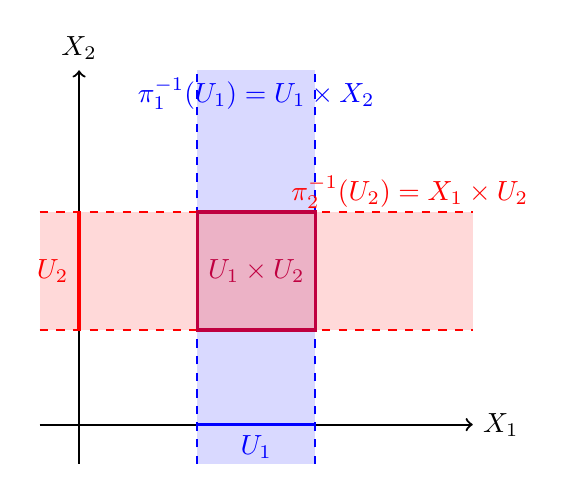
\begin{tikzpicture}[scale=1]
    \draw[->,thick] (-0.5,0) -- (5,0) node[right] {$X_1$};
    \draw[->,thick] (0,-0.5) -- (0,4.5) node[above] {$X_2$};
    
    % Banda vertical \pi_1^{-1}(U_1)
    \fill[blue!15] (1.5,-0.5) rectangle (3,4.5);
    \draw[dashed,blue,thick] (1.5,-0.5) -- (1.5,4.5);
    \draw[dashed,blue,thick] (3,-0.5) -- (3,4.5);
    \node[blue] at (2.25,4.2) {$\pi_1^{-1}(U_1) = U_1 \times X_2$};
    
    % Banda horizontal \pi_2^{-1}(U_2)
    \fill[red!15] (-0.5,1.2) rectangle (5,2.7);
    \draw[dashed,red,thick] (-0.5,1.2) -- (5,1.2);
    \draw[dashed,red,thick] (-0.5,2.7) -- (5,2.7);
    \node[red] at (4.2,2.95) {$\pi_2^{-1}(U_2) = X_1 \times U_2$};
    
    % Intersección U_1 x U_2
    \fill[purple!30] (1.5,1.2) rectangle (3,2.7);
    \draw[purple,very thick] (1.5,1.2) rectangle (3,2.7);
    \node[purple] at (2.25,1.95) {$U_1 \times U_2$};
    
    % Intervalos en los ejes
    \draw[very thick,blue] (1.5,0) -- (3,0) node[midway,below] {$U_1$};
    \draw[very thick,red] (0,1.2) -- (0,2.7) node[midway,left] {$U_2$};
\end{tikzpicture}
\end{center}

\begin{obs}[Topología por cajas vs. Topología producto]
Si en el producto $\prod_{i \in I} X_i$ consideramos la base formada por todos los productos arbitrarios $\prod_{i \in I} U_i$ (sin la restricción de ser $X_i$ para casi todo $i$), se obtiene la \textbf{topología por cajas} (o box topology), denotada $\mc T_{\text{cajas}}$.
\begin{itemize}
    \item En general, $\mc T_\pi \subseteq \mc T_{\text{cajas}}$.
    \item Si el conjunto de índices $I$ es \textbf{finito}, ambas topologías coinciden: $\mc T_\pi = \mc T_{\text{cajas}}$. En particular, en $\mathbb{R}^n = \prod_{i=1}^n \mathbb{R}$, $\mc T_d = \mc T_\pi = \mc T_{\text{cajas}}$.
    \item Si $I$ es \textbf{infinito}, $\mc T_\pi \subsetneq \mc T_{\text{cajas}}$.
\end{itemize}
\end{obs}

\begin{ejem}[Diferencia entre topología producto y por cajas]
Consideremos $X = \mathbb{R}^\mathbb{N} = \prod_{n \in \mathbb{N}} \mathbb{R}$ (el espacio de sucesiones reales). Definamos la aplicación diagonal:
\[
    \Delta \colon (\mathbb{R}, \mc T_d) \longrightarrow \mathbb{R}^\mathbb{N}, \quad x \longmapsto (x, x, x, \ldots).
\]
\begin{itemize}
    \item Con la topología producto $\mc T_\pi$, cada componente $\pi_n \circ \Delta = \operatorname{Id}_\mathbb{R}$ es continua, por lo que por la propiedad universal, $\Delta \colon (\mathbb{R}, \mc T_d) \to (\mathbb{R}^\mathbb{N}, \mc T_\pi)$ es \textbf{continua}.
    \item Con la topología por cajas $\mc T_{\text{cajas}}$, consideremos el abierto por cajas:
    \[
        U = (-1, 1) \times \left(-\frac{1}{2}, \frac{1}{2}\right) \times \ldots \times \left(-\frac{1}{n}, \frac{1}{n}\right) \times \ldots \in \mc T_{\text{cajas}}.
    \]
    Su anti-imagen es $\Delta^{-1}(U) = \bigcap_{n=1}^\infty (-\nicefrac{1}{n}, \nicefrac{1}{n}) = \{0\}$, que \textbf{no} es abierto en $(\mathbb{R}, \mc T_d)$. Así, $\Delta \colon (\mathbb{R}, \mc T_d) \to (\mathbb{R}^\mathbb{N}, \mc T_{\text{cajas}})$ \textbf{no es continua}.
\end{itemize}
\end{ejem}

\subsection*{Topología final}

\begin{defi}
Sea $(X, \mc T_X)$ un espacio topológico, $Y$ un conjunto y $f \colon X \to Y$ una aplicación. La \textbf{topología final} en $Y$ inducida por $f$, denotada $\mc T^f$, es la mayor topología en $Y$ que hace continua a $f$:
\[
    \mc T^f = \{V \subseteq Y \mid f^{-1}(V) \in \mc T_X\}.
\]
Para una familia de aplicaciones $\{f_i \colon (X_i, \mc T_{X_i}) \to Y\}_{i \in I}$, la \textbf{topología final} $\mc T^{\{f_i\}}$ es la mayor topología en $Y$ que hace continuas a todas las $f_i$:
\[
    \mc T^{\{f_i\}} = \bigcap_{i \in I} \mc T^{f_i} = \{V \subseteq Y \mid f_i^{-1}(V) \in \mc T_{X_i}, \; \forall i \in I\}.
\]
\end{defi}

\begin{teo}[Propiedad universal de la topología final]
Sea $Y$ dotado de la topología final $\mc T^{\{f_i\}}$. Para cualquier espacio topológico $(Z, \mc T_Z)$, una aplicación $g \colon (Y, \mc T^{\{f_i\}}) \to (Z, \mc T_Z)$ es continua si y solo si la composición:
\[
    g \circ f_i \colon (X_i, \mc T_{X_i}) \longrightarrow (Z, \mc T_Z)
\]
es continua para todo $i \in I$.
\end{teo}

\begin{dem}
\begin{itemize}
    \item[($\Rightarrow$)] Si $g$ es continua, al ser cada $f_i$ continua, $g \circ f_i$ es continua.
    \item[($\Leftarrow$)] Sea $U \subseteq Z$ abierto. Para ver que $g^{-1}(U) \in \mc T^{\{f_i\}}$, debemos comprobar que $f_i^{-1}(g^{-1}(U)) \in \mc T_{X_i}$ para todo $i \in I$. Pero $f_i^{-1}(g^{-1}(U)) = (g \circ f_i)^{-1}(U)$, que es abierto por ser $g \circ f_i$ continua.
\end{itemize}
\end{dem}

\subsection*{Unión disjunta (Suma topológica)}

\begin{defi}
Dada una familia de espacios topológicos $\{(X_i, \mc T_{X_i})\}_{i \in I}$, el \textbf{espacio unión disjunta} es el coproducto de conjuntos $\coprod_{i \in I} X_i = \{(i, x) \mid i \in I, \; x \in X_i\}$ dotado de la \textbf{topología final} inducida por las inyecciones canónicas:
\[
    \varphi_j \colon X_j \longhookrightarrow \coprod_{i \in I} X_i, \quad x_j \longmapsto (j, x_j).
\]
Un subconjunto $W \subseteq \coprod_{i \in I} X_i$ es abierto si y solo si $\varphi_i^{-1}(W)$ es abierto en $X_i$ para todo $i \in I$. Cada inyección canónica $\varphi_j$ es una inmersión abierta y cerrada.
\end{defi}

\section{Topología cociente}

\begin{defi}
Sea $(X, \mc T_X)$ un espacio topológico y $R$ una relación de equivalencia en $X$. Denotemos por $\pi \colon X \to X/R$ la proyección natural al cociente ($x \mapsto [x]_R$). La \textbf{topología cociente} $\mc T_{X/R}$ es la \textbf{topología final} inducida por $\pi$:
\[
    \mc T_{X/R} = \{V \subseteq X/R \mid \pi^{-1}(V) \in \mc T_X\}.
\]
\end{defi}

\begin{defi}
Sea $R$ una relación de equivalencia en $X$. Un subconjunto $A \subseteq X$ se dice \textbf{saturado} por $R$ si contiene todas las clases de equivalencia de sus elementos:
\[
    \forall a \in A, \quad [a]_R \subseteq A \iff \pi^{-1}(\pi(A)) = A.
\]
Dado cualquier subconjunto $A \subseteq X$, la \textbf{saturación} de $A$ es el menor saturado que contiene a $A$:
\[
    [A]_R \coloneqq \bigcup_{a \in A} [a]_R = \pi^{-1}(\pi(A)).
\]
\end{defi}

\begin{prop}
La proyección canónica $\pi \colon (X, \mc T_X) \to (X/R, \mc T_{X/R})$ es abierta si y solo si para todo abierto $U \in \mc T_X$, su saturado $[U]_R$ es abierto en $X$.
\end{prop}

\begin{dem}
$\pi(U)$ es abierto en el cociente $\iff \pi^{-1}(\pi(U)) \in \mc T_X \iff [U]_R \in \mc T_X$.
\end{dem}

\begin{ejem}[La recta con dos orígenes]
Consideremos dos copias de la recta real $X = \mathbb{R}_1 \sqcup \mathbb{R}_2$. En $X$ definimos la relación de equivalencia que identifica cada punto $x \in \mathbb{R}_1 \setminus \{0\}$ con su homólogo en $\mathbb{R}_2 \setminus \{0\}$:
\[
    (1, x) \sim (2, y) \iff x = y \ne 0.
\]
En el espacio cociente $X/{\sim}$, el espacio es localmente idéntico a la recta real euclídea salvo en el origen, donde existen dos puntos distintos $0_1 = [(1, 0)]$ y $0_2 = [(2, 0)]$. Este espacio \textbf{no es de Hausdorff ($T_2$)}, pues todo entorno abierto de $0_1$ y todo entorno abierto de $0_2$ intersecan fuera del origen.

\begin{center}
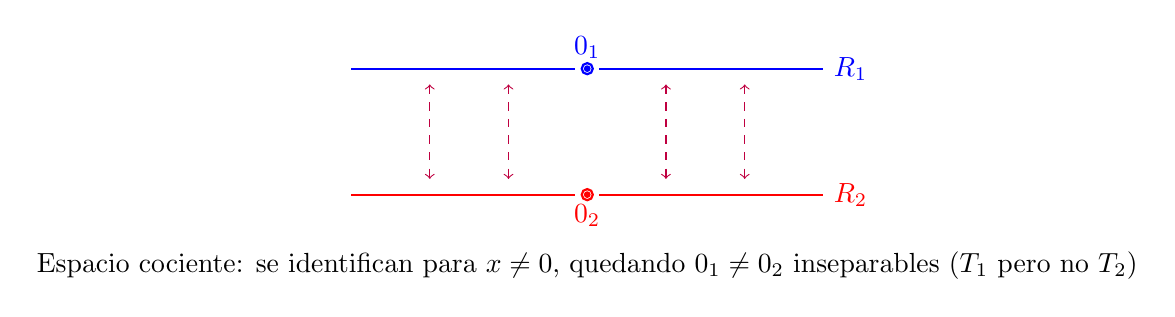
\begin{tikzpicture}[scale=1]
    % Recta R_1 arriba
    \draw[thick,blue] (-3,0.8) -- (-0.15,0.8);
    \draw[thick,blue] (0.15,0.8) -- (3,0.8) node[right] {$\mathbb{R}_1$};
    \draw[thick,blue] (0,0.8) circle (2pt);
    \filldraw[blue] (0,0.8) circle (1pt) node[above] {$0_1$};
    
    % Recta R_2 abajo
    \draw[thick,red] (-3,-0.8) -- (-0.15,-0.8);
    \draw[thick,red] (0.15,-0.8) -- (3,-0.8) node[right] {$\mathbb{R}_2$};
    \draw[thick,red] (0,-0.8) circle (2pt);
    \filldraw[red] (0,-0.8) circle (1pt) node[below] {$0_2$};
    
    % Flechas de pegamiento
    \draw[<->,dashed,purple] (-2,0.6) -- (-2,-0.6);
    \draw[<->,dashed,purple] (-1,0.6) -- (-1,-0.6);
    \draw[<->,dashed,purple] (1,0.6) -- (1,-0.6);
    \draw[<->,dashed,purple] (2,0.6) -- (2,-0.6);
    
    \node at (0,-1.7) [align=center] {Espacio cociente: se identifican para $x \ne 0$, quedando $0_1 \ne 0_2$ inseparables ($T_1$ pero no $T_2$)};
\end{tikzpicture}
\end{center}
\end{ejem}
























\chapter{Espacios m\'etricos}
\section{Métricas, seudométricas e isometrías}

\begin{defi}
Sea $X$ un conjunto. Una \textbf{métrica} (o distancia) en $X$ es una aplicación $d \colon X \times X \to \mathbb{R}$ tal que:
\begin{enumerate}
    \item[\textbf{1)}] $d(x, y) \ge 0$ para todos $x, y \in X$, y $d(x, y) = 0 \iff x = y$.
    \item[\textbf{2)}] $d(x, y) = d(y, x)$ para todos $x, y \in X$ (simetría).
    \item[\textbf{3)}] $d(x, y) \le d(x, z) + d(z, y)$ para todos $x, y, z \in X$ (desigualdad triangular).
\end{enumerate}
Una aplicación $d$ es una \textbf{seudométrica} si verifica las propiedades 2, 3 y la versión debilitada de 1: $d(x, y) \ge 0$ con $x = y \Rightarrow d(x, y) = 0$ (pudiendo ser $d(x, y) = 0$ para puntos distintos $x \ne y$). El par $(X, d)$ se denomina \textbf{espacio métrico} (o seudométrico).
\end{defi}

\begin{ejem}
En $\mathbb{R}^n$, la distancia euclídea usual:
\[
    d(x, y) = \sqrt{\sum_{i=1}^n (x_i - y_i)^2}
\]
es una métrica.
\end{ejem}

\begin{propi}[Métrica acotada asociada]
Sea $(X, d)$ un espacio métrico (o seudométrico). La aplicación:
\[
    \overline{d} \colon X \times X \longrightarrow \mathbb{R}, \quad (x, y) \longmapsto \overline{d}(x, y) \coloneqq \min\{d(x, y), 1\}
\]
es una métrica (o seudométrica) acotada por $1$.
\end{propi}

\begin{dem}
\begin{itemize}
    \item Claramente $\overline{d}(x, y) \ge 0$, y $\overline{d}(x, y) = 0 \iff d(x, y) = 0 \iff x = y$.
    \item Simetría: $\overline{d}(x, y) = \min\{d(x, y), 1\} = \min\{d(y, x), 1\} = \overline{d}(y, x)$.
    \item Desigualdad triangular: Si $\overline{d}(x, z) = 1$ o $\overline{d}(z, y) = 1$, entonces $\overline{d}(x, z) + \overline{d}(z, y) \ge 1 \ge \overline{d}(x, y)$. Si ambos son menores que $1$, $\overline{d}(x, z) = d(x, z)$ y $\overline{d}(z, y) = d(z, y)$, por lo que $\overline{d}(x, y) \le d(x, y) \le d(x, z) + d(z, y) = \overline{d}(x, z) + \overline{d}(z, y)$.
\end{itemize}
\end{dem}

\begin{defi}
Una \textbf{isometría} entre dos espacios métricos $(X, d)$ e $(Y, d')$ es una aplicación $f \colon X \to Y$ que preserva distancias:
\[
    \forall x, x' \in X, \quad d'(f(x), f(x')) = d(x, x').
\]
Si $d$ es métrica, toda isometría es \textbf{inyectiva}:
\[
    f(x) = f(x') \Rightarrow d'(f(x), f(x')) = 0 \Rightarrow d(x, x') = 0 \Rightarrow x = x'.
\]
Dos espacios métricos son \textbf{isomorfos métricamente} (o isométricos) si existe una isometría biyectiva entre ellos.
\end{defi}

\begin{defi}
Sea $(X, d)$ un espacio métrico. Un subconjunto $A \subseteq X$ es \textbf{acotado} si existe $M \in \mathbb{R}^+$ tal que para todos $a, a' \in A$, $d(a, a') \le M$.
\end{defi}

\begin{defi}
Dado $A \subseteq (X, d)$ no vacío y $x \in X$, la distancia de $x$ a $A$ es:
\[
    d(x, A) \coloneqq \inf\{d(x, a) \mid a \in A\}.
\]
Esto induce una función $d_A \colon X \to \mathbb{R}$ dada por $x \mapsto d(x, A)$.
\end{defi}

\begin{center}
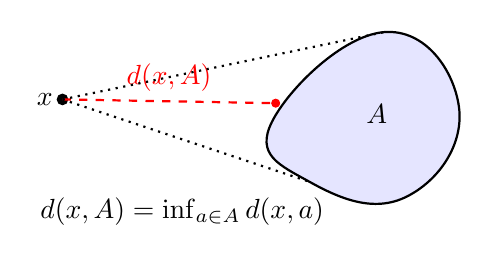
\begin{tikzpicture}[scale=0.95]
    \draw[thick,fill=blue!10] plot[smooth cycle,tension=0.8] coordinates {(2,0) (3.5,1.2) (4.5,0.2) (3.8,-1) (2.5,-0.8)};
    \node at (3.4,0.1) {$A$};
    \filldraw[black] (-0.8,0.3) circle (2pt) node[left] {$x$};
    \draw[dashed,thick,red] (-0.8,0.3) -- (2.05,0.25) node[midway,above] {$d(x, A)$};
    \filldraw[red] (2.05,0.25) circle (1.5pt);
    \draw[dotted,thick] (-0.8,0.3) -- (3.5,1.2);
    \draw[dotted,thick] (-0.8,0.3) -- (2.5,-0.8);
    \node at (0.8,-1.2) [align=center] {$d(x, A) = \inf_{a \in A} d(x, a)$};
\end{tikzpicture}
\end{center}

\begin{ejem}
$\mathbb{N} \subset (\mathbb{R}, d)$ no está acotado. En cambio, en $(\mathbb{R}, \overline{d})$, $\mathbb{N}$ (y todo subconjunto de $\mathbb{R}$) está acotado por $1$.
\end{ejem}

\section{Topología asociada a una métrica}

\begin{defi}
Sea $(X, d)$ un espacio métrico. Dados $x \in X$ y $r \in \mathbb{R}^+$, la \textbf{bola abierta} de centro $x$ y radio $r$ es:
\[
    B_d(x, r) \coloneqq \{y \in X \mid d(x, y) < r\}.
\]
La familia $\{B_d(x, r)\}_{r > 0}$ constituye una base de entornos en $x$, y la colección de todas las bolas abiertas forma una base de una topología en $X$, denominada la \textbf{topología métrica} $\mc T_d$. Un subconjunto $U \subseteq X$ es abierto en $\mc T_d$ si:
\[
    \forall x \in U, \; \exists r_x > 0 \text{ tal que } B_d(x, r_x) \subseteq U.
\]
\end{defi}

\begin{propi}
Toda bola abierta $B_d(x, r)$ es un conjunto abierto en $(X, \mc T_d)$.
\end{propi}

\begin{dem}
Sea $y \in B_d(x, r)$, luego $d(x, y) < r$. Tomando $r_y \coloneqq r - d(x, y) > 0$, para cualquier $z \in B_d(y, r_y)$ se tiene por desigualdad triangular $d(x, z) \le d(x, y) + d(y, z) < d(x, y) + r_y = r$, de donde $B_d(y, r_y) \subseteq B_d(x, r)$.
\end{dem}

\begin{center}
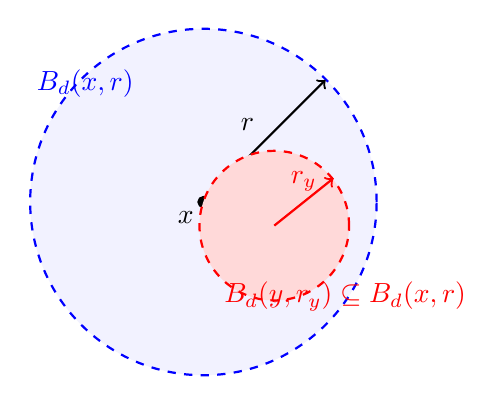
\begin{tikzpicture}[scale=1]
    \draw[thick,blue,dashed,fill=blue!5] (0,0) circle (2.2cm);
    \filldraw[black] (0,0) circle (2pt) node[below left] {$x$};
    \draw[->,thick] (0,0) -- (1.55,1.55) node[midway,above left] {$r$};
    \node[blue] at (-1.5,1.5) {$B_d(x, r)$};
    
    \filldraw[black] (0.9,-0.3) circle (2pt) node[below left] {$y$};
    \draw[thick,red,dashed,fill=red!15] (0.9,-0.3) circle (0.95cm);
    \draw[->,thick,red] (0.9,-0.3) -- (1.65,0.3) node[midway,above] {$r_y$};
    \node[red] at (1.8,-1.2) {$B_d(y, r_y) \subseteq B_d(x, r)$};
\end{tikzpicture}
\end{center}

\begin{defi}
Se define la \textbf{bola cerrada} y la \textbf{esfera} (o circunferencia métrica) de centro $x$ y radio $r$ como:
\begin{align*}
    \overline{B}_d(x, r) &\coloneqq \{y \in X \mid d(x, y) \le r\}, \\
    C_d(x, r) &\coloneqq \{y \in X \mid d(x, y) = r\}.
\end{align*}
Nótese que $\overline{B}_d(x, r) = B_d(x, r) \cup C_d(x, r)$.
\end{defi}

\begin{prop}
La bola cerrada $\overline{B}_d(x, r)$ es un conjunto cerrado en $(X, \mc T_d)$.
\end{prop}

\begin{dem}
Basta ver que su complementario $X \setminus \overline{B}_d(x, r) = \{y \in X \mid d(x, y) > r\}$ es abierto. Si $y \in X \setminus \overline{B}_d(x, r)$, tomamos $r_y \coloneqq d(x, y) - r > 0$. Para todo $z \in B_d(y, r_y)$, $d(x, y) \le d(x, z) + d(z, y) < d(x, z) + r_y$, luego $d(x, z) > d(x, y) - r_y = r$, de modo que $B_d(y, r_y) \subseteq X \setminus \overline{B}_d(x, r)$.
\end{dem}

\begin{obs}
En general, el cierre de la bola abierta está contenido en la bola cerrada: $\overline{B_d(x, r)} \subseteq \overline{B}_d(x, r)$, pero \textbf{no siempre} coinciden. Por ejemplo, en $(\mathbb{R}^n, \overline{d})$, $B_{\overline{d}}(0, 2) = \mathbb{R}^n$, luego $\overline{B_{\overline{d}}(0, 2)} = \mathbb{R}^n$, mientras que para métricas discretas pueden diferir estrictamente.
\end{obs}

\begin{cor}
La familia de bolas cerradas $\{\overline{B}_d(x, r)\}_{r > 0}$ forma una base de entornos cerrados de $x$.
\end{cor}

\section{Espacios metrizables}

\begin{defi}
Un espacio topológico $(X, \mc T)$ es \textbf{metrizable} si existe una métrica $d$ en $X$ tal que $\mc T = \mc T_d$.
\end{defi}

\begin{teo}[Teorema de metrización de Urysohn]
Todo espacio topológico regular ($T_3$), $T_0$ y con base numerable de abiertos (segundo contable) es metrizable.
\end{teo}

\begin{prop}
Sea $(X, d)$ un espacio métrico y $\overline{d}(x, y) = \min\{1, d(x, y)\}$. Entonces:
\[
    \mc T_d = \mc T_{\overline{d}}.
\]
\end{prop}

\begin{dem}
Como $\overline{d}(x, y) \le d(x, y)$, para $r \le 1$ se tiene $B_d(x, r) = B_{\overline{d}}(x, r)$, lo que muestra que ambas métricas generan las mismas bolas para radios pequeños y por tanto la misma topología.
\end{dem}

\begin{prop}
Si $(X, \mc T)$ es metrizable ($\mc T = \mc T_d$ para una seudométrica $d$), son equivalentes:
\begin{enumerate}
    \item[\textbf{1)}] $(X, \mc T)$ es $T_2$ (Hausdorff).
    \item[\textbf{2)}] $(X, \mc T)$ es $T_0$.
    \item[\textbf{3)}] $d$ es métrica.
\end{enumerate}
\end{prop}

\begin{dem}
$1 \Rightarrow 2$ es general. Para $2 \Rightarrow 3$: si $x \ne y$, por ser $T_0$ existe un entorno abierto de uno que no contiene al otro, luego existe $\varepsilon > 0$ con $y \notin B_d(x, \varepsilon)$, lo que implica $d(x, y) \ge \varepsilon > 0$. Para $3 \Rightarrow 1$: si $x \ne y$, como $d$ es métrica $\varepsilon \coloneqq d(x, y) > 0$. Las bolas $B_d(x, \varepsilon/2)$ y $B_d(y, \varepsilon/2)$ son disjuntas por desigualdad triangular, luego $X$ es $T_2$.
\end{dem}

\begin{center}
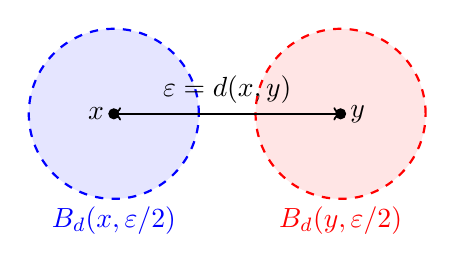
\begin{tikzpicture}[scale=0.9]
    \draw[thick,blue,dashed,fill=blue!10] (0,0) circle (1.2cm);
    \draw[thick,red,dashed,fill=red!10] (3.2,0) circle (1.2cm);
    \filldraw[black] (0,0) circle (2pt) node[left] {$x$};
    \filldraw[black] (3.2,0) circle (2pt) node[right] {$y$};
    \draw[<->,thick] (0,0) -- (3.2,0) node[midway,above] {$\varepsilon = d(x, y)$};
    \node[blue] at (0,-1.5) {$B_d(x, \varepsilon/2)$};
    \node[red] at (3.2,-1.5) {$B_d(y, \varepsilon/2)$};
\end{tikzpicture}
\end{center}

\subsection*{Sucesiones y caracterizaciones secuenciales}

\begin{prop}
En un espacio métrico $(X, d)$, una sucesión $\{x_n\}$ converge a $x \iff \lim_{n \to \infty} d(x, x_n) = 0$.
\end{prop}

\begin{prop}
Sea $(X, \mc T_d)$ un espacio metrizable y $A \subseteq X$. Un punto $x \in \overline{A} \iff$ existe una sucesión $\{x_n\} \subseteq A$ tal que $\lim_{n \to \infty} x_n = x$.
\end{prop}

\begin{dem}
($\Rightarrow$) Para cada $n \in \mathbb{N}$, como $x \in \overline{A}$, la bola $B_d(x, \nicefrac{1}{n})$ corta a $A$. Escogiendo $x_n \in B_d(x, \nicefrac{1}{n}) \cap A$, se construye una sucesión $\{x_n\} \subseteq A$ con $d(x, x_n) < \nicefrac{1}{n} \to 0$.

($\Leftarrow$) Es válido en cualquier espacio topológico: si $x_n \to x$ con $\{x_n\} \subseteq A$, todo entorno de $x$ contiene puntos de $\{x_n\} \subseteq A$, luego $x \in \overline{A}$.
\end{dem}

\begin{prop}
Sean $(X, \mc T_X)$ un espacio metrizable e $(Y, \mc T_Y)$ un espacio topológico arbitrario. Una aplicación $f \colon X \to Y$ es continua si y solo si para toda sucesión $\{x_n\} \subseteq X$ que converge a $x$, la sucesión $\{f(x_n)\}$ converge a $f(x)$ en $Y$.
\end{prop}

\begin{dem}
($\Rightarrow$) Si $f$ es continua y $W$ es entorno de $f(x)$, $f^{-1}(W)$ es entorno de $x$. Como $x_n \to x$, existe $n_0$ con $x_n \in f^{-1}(W)$ para todo $n \ge n_0$, luego $f(x_n) \in W$.

($\Leftarrow$) Sea $C \subseteq Y$ cerrado. Si probamos que $\overline{f^{-1}(C)} = f^{-1}(C)$, habremos demostrado que $f^{-1}(C)$ es cerrado. Sea $x \in \overline{f^{-1}(C)}$; por la caracterización secuencial existe $\{x_n\} \subseteq f^{-1}(C)$ con $x_n \to x$. Entonces $\{f(x_n)\} \subseteq C$, y por hipótesis $f(x_n) \to f(x)$. Como $C$ es cerrado, $f(x) \in C$, luego $x \in f^{-1}(C)$.
\end{dem}

\begin{prop}
Sean $(X, d)$ e $(Y, d')$ espacios métricos. Una aplicación $f \colon X \to Y$ es continua $\iff$ para todo $x \in X$ y todo $\varepsilon > 0$, existe $\delta_{x, \varepsilon} > 0$ tal que:
\[
    d(x, x') < \delta_{x, \varepsilon} \Rightarrow d'(f(x), f(x')) < \varepsilon \iff B_d(x, \delta_{x, \varepsilon}) \subseteq f^{-1}(B_{d'}(f(x), \varepsilon)).
\]
\end{prop}

\section{Continuidad uniforme y separabilidad}

\begin{defi}
Una aplicación $f \colon (X, d) \to (Y, d')$ es \textbf{uniformemente continua} si para todo $\varepsilon > 0$ existe $\delta_\varepsilon > 0$ (independiente del punto $x$) tal que:
\[
    \forall x, x' \in X, \quad d(x, x') < \delta_\varepsilon \Rightarrow d'(f(x), f(x')) < \varepsilon.
\]
Toda aplicación uniformemente continua es continua.
\end{defi}

\begin{propi}
Sea $(X, d)$ un espacio métrico y $A \subseteq X$ no vacío. La función distancia al subconjunto:
\[
    d_A \colon X \longrightarrow \mathbb{R}, \quad x \longmapsto d(x, A) = \inf_{a \in A} d(x, a)
\]
es uniformemente continua (y en particular, continua).
\end{propi}

\begin{dem}
Para cualesquiera $x, x' \in X$ y $a \in A$: $d(x, a) \le d(x, x') + d(x', a)$. Tomando ínfimo sobre $a \in A$, $d(x, A) \le d(x, x') + d(x', a)$, de donde $d(x, A) - d(x', A) \le d(x, x')$. Por simetría:
\[
    |d(x, A) - d(x', A)| \le d(x, x').
\]
Basta tomar $\delta_\varepsilon = \varepsilon$.
\end{dem}

\begin{defi}
Un espacio topológico $X$ es \textbf{separable} si contiene un subconjunto denso y numerable: existe $Y \subseteq X$ numerable tal que $\overline{Y} = X$.
\end{defi}

\begin{ejem}
$\mathbb{R}$ es separable, pues $\mathbb{Q} \subset \mathbb{R}$ es numerable y $\overline{\mathbb{Q}} = \mathbb{R}$.
\end{ejem}

\begin{propi}
Todo espacio métrico separable $(X, d)$ tiene una base numerable de abiertos (es segundo contable).
\end{propi}

\begin{dem}
Sea $Y = \{x_n\}_{n \in \mathbb{N}}$ un subconjunto numerable denso en $X$. Consideremos la familia numerable de bolas:
\[
    \mathcal{B} = \{B_d(x_n, 1/m) \mid n, m \in \mathbb{N}\}.
\]
Dado cualquier abierto $U$ y $x \in U$, existe $r > 0$ con $B_d(x, r) \subseteq U$. Tomando $m \in \mathbb{N}$ tal que $1/m < r/2$, por la densidad de $Y$ existe $x_n \in Y$ con $d(x, x_n) < 1/m$. Entonces $x \in B_d(x_n, 1/m) \subseteq B_d(x, r) \subseteq U$. Luego $\mathcal{B}$ es base numerable.
\end{dem}

\begin{cor}
$\mathbb{R}^n$ es separable (mediante $\mathbb{Q}^n$) y tiene base numerable de abiertos: $\{B_d(q, 1/m) \mid q \in \mathbb{Q}^n, \; m \in \mathbb{N}\}$.
\end{cor}

\section{Espacios métricos $\mathbb{R}^n$ y métricas equivalentes}

\begin{teo}
$(\mathbb{R}^n, \mc T_\pi)$ es metrizable.
\end{teo}

\begin{dem}
Definimos la distancia del máximo en $\mathbb{R}^n$:
\[
    d_{\max}(x, y) \coloneqq \max_{1 \le i \le n} |x_i - y_i|.
\]
Probemos que $\mc T_\pi = \mc T_{d_{\max}}$:
\begin{itemize}
    \item[($\subseteq$)] Sea $U = U_1 \times \ldots \times U_n \in \mc T_\pi$ un abierto básico y $x \in U$. Para cada $i$, como $U_i \in \mc T_d$, existe $\varepsilon_i > 0$ tal que $(x_i - \varepsilon_i, x_i + \varepsilon_i) \subseteq U_i$. Tomando $\varepsilon = \min_{1 \le i \le n} \varepsilon_i > 0$, si $y \in B_{d_{\max}}(x, \varepsilon)$, entonces $|x_i - y_i| \le d_{\max}(x, y) < \varepsilon \le \varepsilon_i$, luego $y_i \in U_i$ para todo $i$, y $B_{d_{\max}}(x, \varepsilon) \subseteq U$.
    \item[($\supseteq$)] Sea $x \in \mathbb{R}^n$ y $\varepsilon > 0$. El producto $U = B_{d_1}(x_1, \varepsilon) \times \ldots \times B_{d_1}(x_n, \varepsilon)$ es un abierto básico de $\mc T_\pi$ que contiene a $x$ y cumple $U \subseteq B_{d_{\max}}(x, \varepsilon)$.
\end{itemize}
\end{dem}

\begin{prop}
En $\mathbb{R}^n$ consideramos las siguientes cuatro métricas:
\begin{enumerate}
    \item[\textbf{a)}] $d(x, y) = \sqrt{\sum_{i=1}^n |x_i - y_i|^2}$ (euclídea).
    \item[\textbf{b)}] $\overline{d}(x, y) = \min\{1, d(x, y)\}$.
    \item[\textbf{c)}] $d_{\max}(x, y) = \max_{1 \le i \le n} |x_i - y_i|$.
    \item[\textbf{d)}] $d_{\text{suma}}(x, y) = \sum_{i=1}^n |x_i - y_i|$ (de Manhattan).
\end{enumerate}
Todas ellas inducen la misma topología:
\[
    \mc T_{\overline{d}} = \mc T_d = \mc T_{d_{\text{suma}}} = \mc T_{d_{\max}} = \mc T_\pi.
\]
\end{prop}

\begin{dem}
Para todos $x, y \in \mathbb{R}^n$:
\[
    d_{\max}^2(x, y) = \max_{1 \le i \le n} |x_i - y_i|^2 \le \sum_{i=1}^n |x_i - y_i|^2 = d^2(x, y) \le \left(\sum_{i=1}^n |x_i - y_i|\right)^2 = d_{\text{suma}}^2(x, y).
\]
Tomando raíces cuadradas: $d_{\max}(x, y) \le d(x, y) \le d_{\text{suma}}(x, y)$. Además:
\[
    d_{\text{suma}}(x, y) = \sum_{i=1}^n |x_i - y_i| \le n \max_{1 \le i \le n} |x_i - y_i| = n \, d_{\max}(x, y).
\]
Por tanto, $B_{d_{\text{suma}}}(x, \varepsilon) \subseteq B_d(x, \varepsilon) \subseteq B_{d_{\max}}(x, \varepsilon)$, y $B_{d_{\max}}(x, \varepsilon/n) \subseteq B_{d_{\text{suma}}}(x, \varepsilon)$, lo que demuestra que las topologías coinciden.
\end{dem}

\begin{center}
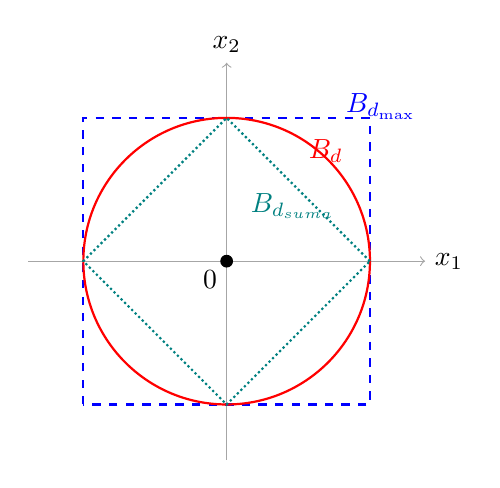
\begin{tikzpicture}[scale=1.4]
    \draw[->,gray!70] (-1.8,0) -- (1.8,0) node[right,black] {$x_1$};
    \draw[->,gray!70] (0,-1.8) -- (0,1.8) node[above,black] {$x_2$};
    
    % Bola máximo (cuadrado)
    \draw[thick,blue,dashed] (-1.3,-1.3) rectangle (1.3,1.3);
    \node[blue] at (1.4,1.4) {$B_{d_{\max}}$};
    
    % Bola euclídea (círculo)
    \draw[thick,red] (0,0) circle (1.3cm);
    \node[red] at (0.9,1) {$B_d$};
    
    % Bola suma (rombo)
    \draw[thick,teal,densely dotted] (1.3,0) -- (0,1.3) -- (-1.3,0) -- (0,-1.3) -- cycle;
    \node[teal] at (0.6,0.5) {$B_{d_{\text{suma}}}$};
    
    \filldraw[black] (0,0) circle (1.5pt) node[below left] {$0$};
\end{tikzpicture}
\end{center}

\section{Metrizabilidad de $\mathbb{R}^\mathbb{N}$}

\begin{teo}
El espacio producto numerable $(\mathbb{R}^\mathbb{N}, \mc T_\pi)$ (espacio de sucesiones de números reales dotado de la topología producto) es metrizable.
\end{teo}

\begin{dem}
En $\mathbb{R}$ consideramos la métrica acotada $\overline{d}(a, b) = \min\{1, |a - b|\} \le 1$. Para $x = (x_n)_{n \in \mathbb{N}}$ e $y = (y_n)_{n \in \mathbb{N}}$ en $\mathbb{R}^\mathbb{N}$, definimos:
\[
    D(x, y) \coloneqq \sup_{n \in \mathbb{N}} \left\{ \frac{\overline{d}(x_n, y_n)}{n} \right\} \le 1.
\]
\begin{enumerate}
    \item[\textbf{1)}] $D(x, y) \ge 0$. Si $D(x, y) = 0 \iff \frac{\overline{d}(x_n, y_n)}{n} = 0$ para todo $n \iff x_n = y_n$ para todo $n \iff x = y$.
    \item[\textbf{2)}] Simetría: inmediata por la simetría de $\overline{d}$.
    \item[\textbf{3)}] Desigualdad triangular: Para cada $n \in \mathbb{N}$, $\frac{\overline{d}(x_n, y_n)}{n} \le \frac{\overline{d}(x_n, z_n)}{n} + \frac{\overline{d}(z_n, y_n)}{n} \le D(x, z) + D(z, y)$. Tomando supremo en $n$, $D(x, y) \le D(x, z) + D(z, y)$.
\end{enumerate}
Luego $D$ es una métrica en $\mathbb{R}^\mathbb{N}$. Veamos que $\mc T_\pi = \mc T_D$:
\begin{itemize}
    \item[($\mc T_\pi \subseteq \mc T_D$)] Basta probar que cada abierto de la subbase $\pi_N^{-1}(B_{\overline{d}}(x_N, \varepsilon))$ contiene una bola abierta $B_D(x, \delta)$. Tomando $\delta = \frac{\varepsilon}{N} > 0$: si $y \in B_D(x, \delta)$, entonces $\frac{\overline{d}(x_N, y_N)}{N} \le D(x, y) < \frac{\varepsilon}{N}$, luego $\overline{d}(x_N, y_N) < \varepsilon$, de donde $y \in \pi_N^{-1}(B_{\overline{d}}(x_N, \varepsilon))$.
    \item[($\mc T_D \subseteq \mc T_\pi$)] Sea $x \in \mathbb{R}^\mathbb{N}$ y $\varepsilon > 0$. Elegimos $N \in \mathbb{N}$ tal que $\frac{1}{N} < \varepsilon$. Definimos el abierto de $\mc T_\pi$:
    \[
        U = (x_1 - \varepsilon, x_1 + \varepsilon) \times \ldots \times (x_N - \varepsilon, x_N + \varepsilon) \times \prod_{n > N} \mathbb{R}.
    \]
    Para todo $y \in U$:
    \begin{itemize}
        \item Si $n \le N$: $\frac{\overline{d}(x_n, y_n)}{n} \le \overline{d}(x_n, y_n) < \varepsilon$.
        \item Si $n > N$: $\frac{\overline{d}(x_n, y_n)}{n} \le \frac{1}{n} < \frac{1}{N} < \varepsilon$.
    \end{itemize}
    Por tanto, $D(x, y) = \sup_{n} \frac{\overline{d}(x_n, y_n)}{n} \le \varepsilon$, lo que implica $U \subseteq B_D(x, 2\varepsilon)$. Consecuentemente, $\mc T_D = \mc T_\pi$.
\end{itemize}
\end{dem}

\begin{obs}
\begin{itemize}
    \item Con la topología por cajas $\mc T_{\text{cajas}}$, el espacio $(\mathbb{R}^\mathbb{N}, \mc T_{\text{cajas}})$ \textbf{no} es metrizable.
    \item Si el conjunto de índices $I$ no es numerable, el producto $(\mathbb{R}^I, \mc T_\pi)$ \textbf{no} es metrizable.
\end{itemize}
\end{obs}


































\chapter{Espacios conexos}
Sea $X$ un espacio topológico.

\section{Espacios conexos y separaciones}

\begin{defi}
Una \textbf{separación} de un espacio topológico $X$ es un par de abiertos no vacíos y disjuntos $(A, B)$ tales que:
\[
    X = A \cup B, \quad A \ne \emptyset, \; B \ne \emptyset, \quad A \cap B = \emptyset.
\]
Equivalentemente, $A$ y $B$ son subconjuntos complementarios no triviales que son simultáneamente abiertos y cerrados (clopen). Se llama \textbf{separación trivial} a la pareja $(\emptyset, X)$ o $(X, \emptyset)$.
\end{defi}

\begin{defi}
Un espacio topológico $X$ es \textbf{conexo} si no admite ninguna separación no trivial; es decir, los únicos subconjuntos de $X$ que son simultáneamente abiertos y cerrados son $\emptyset$ y $X$.
\end{defi}

\begin{defi}
Un subespacio topológico $Y \subseteq X$ es conexo si lo es dotado de la topología relativa $(Y, \mc T_{X|Y})$.
\end{defi}

\begin{ejem}
\begin{itemize}
    \item La recta real $\mathbb{R}$ dotada de la topología habitual es conexa.
    \item El subespacio $X = [-2, -1] \cup [1, 2] \subset \mathbb{R}$ no es conexo, pues $[-2, -1] = (-3, 0) \cap X$ y $[1, 2] = (0, 3) \cap X$ constituyen una separación no trivial por abiertos relativos.
\end{itemize}
\end{ejem}

\begin{prop}
Sea $Y \subseteq X$ un subespacio conexo y sea $(A, B)$ una separación de $X$. Entonces:
\[
    Y \subseteq A \quad \text{o bien} \quad Y \subseteq B.
\]
\end{prop}

\begin{dem}
Como $X = A \cup B$ con $A \cap B = \emptyset$, tenemos:
\[
    Y = (A \cap Y) \cup (B \cap Y), \quad (A \cap Y) \cap (B \cap Y) = \emptyset.
\]
Al ser $A$ y $B$ abiertos en $X$, $A \cap Y$ y $B \cap Y$ son abiertos en $Y$. Por ser $Y$ conexo, esta separación relativa debe ser trivial, de modo que $A \cap Y = \emptyset$ (y así $Y \subseteq B$) o $B \cap Y = \emptyset$ (y así $Y \subseteq A$).
\end{dem}

\begin{prop}
Sea $Y \subseteq X$ un subespacio conexo. Para todo subespacio $Z \subseteq X$ tal que $Y \subseteq Z \subseteq \overline{Y}$, $Z$ es conexo. En particular, la clausura $\overline{Y}$ de todo subespacio conexo es conexa.
\end{prop}

\begin{dem}
Sea $(A, B)$ una separación de $Z$ por cerrados relativos: $Z = A \cup B$ con $A \cap B = \emptyset$. Existen cerrados $\overline{A}, \overline{B}$ en $X$ con $A = \overline{A} \cap Z$ y $B = \overline{B} \cap Z$. Como $Y \subseteq Z$ es conexo, por la proposición anterior $Y \subseteq A$ o $Y \subseteq B$. Si $Y \subseteq A$, entonces $\overline{Y} \subseteq \overline{A}$, y por tanto:
\[
    Z \subseteq \overline{Y} \cap Z \subseteq \overline{A} \cap Z = A.
\]
Esto implica $B = \emptyset$, por lo que la separación de $Z$ es trivial y $Z$ es conexo.
\end{dem}

\begin{prop}
Sea $\{X_i\}_{i \in I}$ una familia de subespacios conexos de $X$ tales que su intersección común es no vacía: $\bigcap_{i \in I} X_i \ne \emptyset$. Entonces:
\[
    \bigcup_{i \in I} X_i \quad \text{es conexo}.
\]
\end{prop}

\begin{dem}
Sea $(A, B)$ una separación de $\bigcup_{i \in I} X_i$. Fijemos un punto $x \in \bigcap_{i \in I} X_i$. Sin pérdida de generalidad, supongamos $x \in A$. Para cada $j \in I$, como $X_j$ es conexo, $X_j \subseteq A$ o $X_j \subseteq B$. Puesto que $x \in X_j \cap A$, necesariamente $X_j \subseteq A$ para todo $j \in I$. En consecuencia, $\bigcup_{j \in I} X_j \subseteq A$, lo que obliga a $B = \emptyset$.
\end{dem}

\begin{ejem}
Si dos subespacios disjuntos no se cortan, su unión en general no es conexa. Por ejemplo, en $\mathbb{R}^2$ tomemos dos rectas verticales distintas $X_1 = \{x_1\} \times \mathbb{R}$ y $X_2 = \{x_2\} \times \mathbb{R}$ con $x_1 \ne x_2$. La unión $X_1 \cup X_2$ no es conexa.

\begin{center}
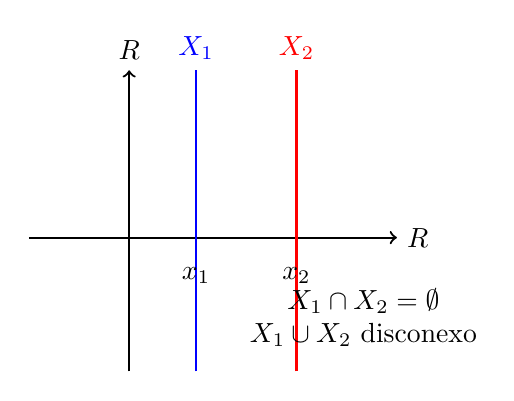
\begin{tikzpicture}[scale=0.85]
    \draw[->,thick] (-1.5,0) -- (4,0) node[right] {$\mathbb{R}$};
    \draw[->,thick] (0,-2) -- (0,2.5) node[above] {$\mathbb{R}$};
    \draw[thick,blue] (1,-2) -- (1,2.5) node[above] {$X_1$};
    \draw[thick,red] (2.5,-2) -- (2.5,2.5) node[above] {$X_2$};
    \node at (1,-0.3) [below] {$x_1$};
    \node at (2.5,-0.3) [below] {$x_2$};
    \node at (3.5,-1.2) [align=center] {$X_1 \cap X_2 = \emptyset$ \\ $X_1 \cup X_2$ disconexo};
\end{tikzpicture}
\end{center}
\end{ejem}

\subsection*{Conexión en la recta real}

\begin{defi}
Un subconjunto $A \subseteq \mathbb{R}$ es un \textbf{intervalo} si para cualesquiera $a, b \in A$ con $a < b$, se verifica $[a, b] \subseteq A$.
\end{defi}

\begin{prop}
Los únicos subespacios conexos de $(\mathbb{R}, \mc T_d)$ son los puntos unitarios y los intervalos.
\end{prop}

\begin{dem}
\begin{itemize}
    \item[($\Rightarrow$)] Sea $A \subseteq \mathbb{R}$ conexo con más de un punto. Si $A$ no fuera un intervalo, existirían $a < b \in A$ y un punto $c \notin A$ tal que $a < c < b$. Entonces $U_1 = (-\infty, c)$ y $U_2 = (c, \infty)$ son abiertos disjuntos de $\mathbb{R}$ que inducen una separación no trivial en $A$:
    \[
        A = (A \cap (-\infty, c)) \cup (A \cap (c, \infty)),
    \]
    ya que $a \in A \cap U_1$ y $b \in A \cap U_2$, contradiciendo que $A$ es conexo.
    \item[($\Leftarrow$)] Todo punto unitario es conexo. Supongamos que $A$ es un intervalo y que $A = U_1 \cup U_2$ con $U_1, U_2$ abiertos relativos disjuntos y no vacíos. Sean $a \in U_1$ y $b \in U_2$ con $a < b$. Como $A$ es intervalo, $[a, b] \subseteq A$. Es suficiente ver que $[a, b] \cong [0, 1]$ es conexo. Supongamos $[0, 1] = U_1 \cup U_2$ con $0 \in U_1$. Sea $r = \sup \{t \in [0, 1] \mid [0, t] \subseteq U_1\}$. Si $r \in U_1$, como $U_1$ es abierto existe $\varepsilon > 0$ con $[r, r+\varepsilon) \subseteq U_1$, contradiciendo que $r$ es cota superior. Si $r \in U_2$, por apertura existe $\varepsilon' > 0$ con $(r-\varepsilon', r] \subseteq U_2$, contradiciendo que $r$ es la menor cota superior. Por tanto, $[0, 1]$ es conexo y todo intervalo es conexo.
\end{itemize}
\end{dem}

\section{Preservación de la conexión y Teorema del Valor Medio}

\begin{prop}
Sea $f \colon X \to Y$ una aplicación continua. Si $X$ es conexo, entonces su imagen $\operatorname{Im}(f) = f(X)$ es un subespacio conexo de $Y$. En particular, si $A \subseteq X$ es conexo, $f(A)$ es conexo en $Y$.
\end{prop}

\begin{dem}
Consideremos la correstricción continua $\tilde{f} \colon X \to \operatorname{Im}(f)$. Si $\operatorname{Im}(f) = V_1 \cup V_2$ fuera una separación abierta no trivial, entonces:
\[
    X = \tilde{f}^{-1}(V_1) \cup \tilde{f}^{-1}(V_2)
\]
sería una separación abierta no trivial de $X$, contradiciendo su conexión.
\end{dem}

\begin{cor}[Teorema del valor intermedio]
Sea $X$ un espacio conexo y $f \colon X \to \mathbb{R}$ continua. Si $a, b \in \operatorname{Im}(f)$ con $a < b$, entonces para todo valor $c \in [a, b]$ existe un punto $x \in X$ tal que $f(x) = c$.
\end{cor}

\begin{dem}
Como $X$ es conexo, su imagen $\operatorname{Im}(f) \subseteq \mathbb{R}$ es conexa, luego es un intervalo. Si $a, b \in \operatorname{Im}(f)$, por definición de intervalo $[a, b] \subseteq \operatorname{Im}(f)$.
\end{dem}

\begin{teo}
Sea $\{X_i\}_{i \in I}$ una familia de espacios topológicos. El producto $\prod_{i \in I} X_i$ es conexo si y solo si cada $X_j$ es conexo.
\end{teo}

\begin{dem}
($\Rightarrow$) Como las proyecciones canónicas $\pi_j \colon \prod X_i \to X_j$ son continuas y sobreyectivas, la imagen $\pi_j(\prod X_i) = X_j$ es conexa.

($\Leftarrow$) Consideremos primero el caso finito $n = 2$: $X_1 \times X_2$. Fijemos un punto base $b = (b_1, b_2) \in X_1 \times X_2$. Para cada $x_1 \in X_1$, el subespacio en forma de ``cruz'':
\[
    C_{x_1} \coloneqq (\{x_1\} \times X_2) \cup (X_1 \times \{b_2\})
\]
es conexo, pues $\{x_1\} \times X_2 \cong X_2$ y $X_1 \times \{b_2\} \cong X_1$ son conexos y se cortan en el punto $(x_1, b_2)$. Además, para todo $x_1 \in X_1$, $b \in C_{x_1}$, por lo que:
\[
    X_1 \times X_2 = \bigcup_{x_1 \in X_1} C_{x_1}
\]
es una unión de conexos con intersección no vacía, luego es conexo.

\begin{center}
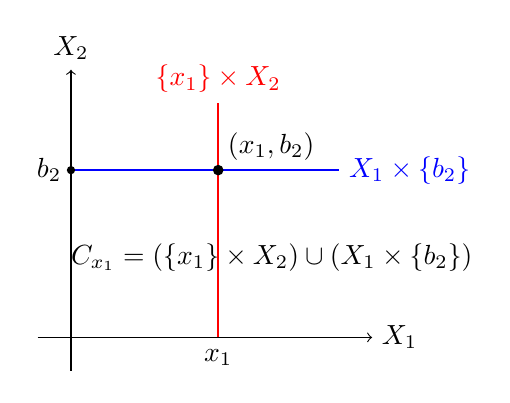
\begin{tikzpicture}[scale=0.85]
    \draw[->] (-0.5,0) -- (4.5,0) node[right] {$X_1$};
    \draw[->] (0,-0.5) -- (0,4) node[above] {$X_2$};
    \draw[thick,blue] (0,2.5) -- (4,2.5) node[right] {$X_1 \times \{b_2\}$};
    \draw[thick,red] (2.2,0) -- (2.2,3.5) node[above] {$\{x_1\} \times X_2$};
    \filldraw[black] (2.2,2.5) circle (2pt) node[above right] {$(x_1, b_2)$};
    \filldraw[black] (0,2.5) circle (1.5pt) node[left] {$b_2$};
    \node at (2.2,-0.3) {$x_1$};
    \node at (3,1.2) [align=center] {$C_{x_1} = (\{x_1\} \times X_2) \cup (X_1 \times \{b_2\})$};
\end{tikzpicture}
\end{center}

Por inducción, todo producto finito $\prod_{i=1}^n X_i$ es conexo. Para $I$ arbitrario, fijemos $b = (b_i)_{i \in I}$. Para cada subconjunto finito $M \subset I$, definimos:
\[
    F^M \coloneqq \left\{(x_i)_{i \in I} \in \prod_{i \in I} X_i \;\middle|\; x_i = b_i, \; \forall i \notin M\right\} \cong \prod_{i \in M} X_i.
\]
Cada $F^M$ es conexo y contiene a $b$. Entonces $Y = \bigcup_{M \subset I \text{ finito}} F^M$ es conexo. Dado cualquier abierto básico no vacío $U$ de la topología producto, $U$ restringe solo un número finito de coordenadas, por lo que corta a algún $F^M \subseteq Y$. Así, $Y$ es denso en $\prod X_i$. Por tanto, $\prod_{i \in I} X_i = \overline{Y}$ es conexo.
\end{dem}

\begin{cor}
$\mathbb{R}^n$ y $\mathbb{R}^\mathbb{N}$ son espacios conexos.
\end{cor}

\begin{obs}
La unión disjunta $\coprod_{i \in I} X_i$ con $|I| \ge 2$ \textbf{nunca} es conexa, pues cada componente $\varphi_j(X_j)$ es abierta y cerrada a la vez.
\end{obs}

\section{Componentes conexas}

Sea $X$ un espacio topológico. Se define la siguiente relación en $X$:
\[
    x \sim y \iff \text{existe un subespacio conexo } A \subseteq X \text{ tal que } x, y \in A.
\]

\begin{propi}
La relación $\sim$ es una relación de equivalencia:
\begin{enumerate}
    \item \textbf{Reflexiva:} $x \sim x$, ya que $\{x\}$ es conexo.
    \item \textbf{Simétrica:} Si $x, y \in A$ conexo, $y, x \in A$.
    \item \textbf{Transitiva:} Si $x \sim y$ ($x, y \in A$ conexo) e $y \sim z$ ($y, z \in B$ conexo), como $y \in A \cap B \ne \emptyset$, $A \cup B$ es conexo y $x, z \in A \cup B$.
\end{enumerate}
\end{propi}

\begin{defi}
Las clases de equivalencia de la relación $\sim$ se denominan \textbf{componentes conexas} de $X$. La componente conexa de un punto $x$ se denota $[x] = C_x$.
\end{defi}

\begin{lema}
Si $A \subseteq X$ es un subespacio conexo y $x \in A$, entonces $A \subseteq [x]$.
\end{lema}

\begin{prop}
Las componentes conexas de $X$ son los subespacios conexos maximales de $X$. Además, son disjuntas y particionan $X$: $X = \coprod C_i$.
\end{prop}

\begin{dem}
Cada clase $[x] = \bigcup \{A \subseteq X \text{ conexo} \mid x \in A\}$ es conexa por ser unión de conexos con el punto $x$ en común. Si $C \subseteq K$ con $K$ conexo, tomando $x \in C$ se tiene $K \subseteq [x] = C$, luego es maximal.
\end{dem}

\begin{prop}
Toda componente conexa $C$ de un espacio topológico $X$ es un conjunto \textbf{cerrado}: $C = \overline{C}$.
\end{prop}

\begin{dem}
Como $C$ es conexo, su clausura $\overline{C}$ es conexa. Por la maximalidad de $C$, $C \subseteq \overline{C} \Rightarrow C = \overline{C}$.
\end{dem}

\begin{obs}
En general, las componentes conexas \textbf{no} son abiertas. Sin embargo, si $X$ tiene un número finito de componentes conexas $X = C_1 \cup \ldots \cup C_n$, entonces cada $C_i = X \setminus \bigcup_{j \ne i} C_j$ es el complementario de una unión finita de cerrados, luego cada $C_i$ es simultáneamente abierta y cerrada.
\end{obs}

\begin{ejem}
\begin{itemize}
    \item En $(X, \mc T_{\text{discreta}})$, los únicos subespacios conexos son los puntos aislados $\{x\}$. Las componentes conexas son los puntos unitarios, por lo que $X$ es \textbf{totalmente disconexo}.
    \item En la recta de Sorgenfrey $(\mathbb{R}, \mc T_{\text{Sorg}})$, para todo punto $a \in Y \subseteq \mathbb{R}$, $Y = (Y \cap (-\infty, a)) \cup (Y \cap [a, \infty))$ define una separación abierta relativa si existen puntos a izquierda y derecha de $a$. Por tanto, $(\mathbb{R}, \mc T_{\text{Sorg}})$ es totalmente disconexo.
\end{itemize}
\end{ejem}

\section{Espacios arcoconexos (Conexión por caminos)}

\begin{defi}
Sea $X$ un espacio topológico y $x, x' \in X$. Un \textbf{camino} (o arco) en $X$ que une $x$ con $x'$ es una aplicación continua:
\[
    \gamma \colon [0, 1] \longrightarrow X \quad \text{tal que } \gamma(0) = x, \; \gamma(1) = x'.
\]
Dados dos caminos continuos $\gamma_1, \gamma_2 \colon [0, 1] \to X$ tales que $\gamma_1(1) = \gamma_2(0) = x'$, se define la \textbf{concatenación} (o suma de caminos) $\gamma_1 * \gamma_2 \colon [0, 1] \to X$:
\[
    (\gamma_1 * \gamma_2)(t) = \begin{cases} \gamma_1(2t) & \text{si } 0 \le t \le \frac{1}{2}, \\ \gamma_2(2t - 1) & \text{si } \frac{1}{2} \le t \le 1. \end{cases}
\]
Por el lema de pegamiento cerrado, $\gamma_1 * \gamma_2$ es continua y define un camino que une $\gamma_1(0)$ con $\gamma_2(1)$.
\end{defi}

\begin{center}
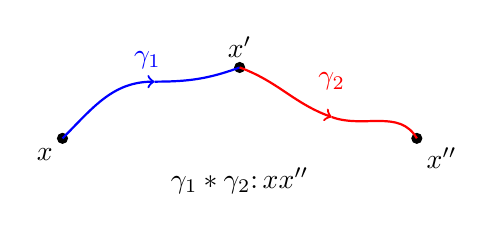
\begin{tikzpicture}[scale=0.9]
    \filldraw[black] (0,0) circle (2pt) node[below left] {$x$};
    \filldraw[black] (2.5,1) circle (2pt) node[above] {$x'$};
    \filldraw[black] (5,0) circle (2pt) node[below right] {$x''$};
    \draw[thick,blue,->] (0,0) to[out=45,in=180] (1.3,0.8);
    \draw[thick,blue] (1.3,0.8) to[out=0,in=200] (2.5,1);
    \node[blue] at (1.2,1.1) {$\gamma_1$};
    \draw[thick,red,->] (2.5,1) to[out=-20,in=160] (3.8,0.3);
    \draw[thick,red] (3.8,0.3) to[out=-20,in=120] (5,0);
    \node[red] at (3.8,0.8) {$\gamma_2$};
    \node at (2.5,-0.6) {$\gamma_1 * \gamma_2 \colon x \rightsquigarrow x''$};
\end{tikzpicture}
\end{center}

\begin{defi}
Un espacio topológico $X$ es \textbf{arcoconexo} (o conexo por caminos) si para cualesquiera dos puntos $x, x' \in X$, existe un camino en $X$ que une $x$ con $x'$.
\end{defi}

\begin{teo}
Todo espacio arcoconexo es conexo.
\end{teo}

\begin{dem}
Supongamos que $X$ admite una separación no trivial $X = U \cup U'$ con $U \cap U' = \emptyset$ y $U, U' \ne \emptyset$. Sean $x \in U$ y $x' \in U'$. Como $X$ es arcoconexo, existe un camino continuo $\gamma \colon [0, 1] \to X$ con $\gamma(0) = x$ y $\gamma(1) = x'$. La imagen $\gamma([0, 1])$ es conexa, pero:
\[
    \gamma([0, 1]) = (\gamma([0, 1]) \cap U) \cup (\gamma([0, 1]) \cap U')
\]
constituye una separación no trivial de $\gamma([0, 1])$, contradicción.
\end{dem}

\begin{prop}
Si $f \colon X \to Y$ es continua y $X$ es arcoconexo, $\operatorname{Im}(f)$ es un subespacio arcoconexo de $Y$.
\end{prop}

\begin{dem}
Dados $y, y' \in \operatorname{Im}(f)$, existen $x, x' \in X$ con $f(x) = y$ y $f(x') = y'$. Si $\gamma \colon [0, 1] \to X$ es un camino entre $x$ y $x'$, entonces $f \circ \gamma \colon [0, 1] \to \operatorname{Im}(f)$ es continua y une $y$ con $y'$.
\end{dem}

\begin{ejem}[Contraejemplos: conexo $\not\Rightarrow$ arcoconexo]
\textbf{1. Seno del topólogo:} Sea $\Gamma_f$ la gráfica de $f(x) = \sin(1/x)$ en $(0, \infty)$:
\[
    \Gamma_f = \left\{\left(x, \sin\frac{1}{x}\right) \;\middle|\; x > 0\right\} \subset \mathbb{R}^2.
\]
$\Gamma_f$ es arcoconexo (es imagen continua de $(0, \infty)$), luego conexo. Su clausura en $\mathbb{R}^2$ es:
\[
    \overline{\Gamma}_f = \Gamma_f \cup (\{0\} \times [-1, 1]).
\]
$\overline{\Gamma}_f$ es conexo (por ser clausura de un conexo), pero \textbf{no es arcoconexo}: no existe ningún camino continuo que conecte el origen $(0, 0)$ con un punto de la gráfica $\Gamma_f$.

\begin{center}
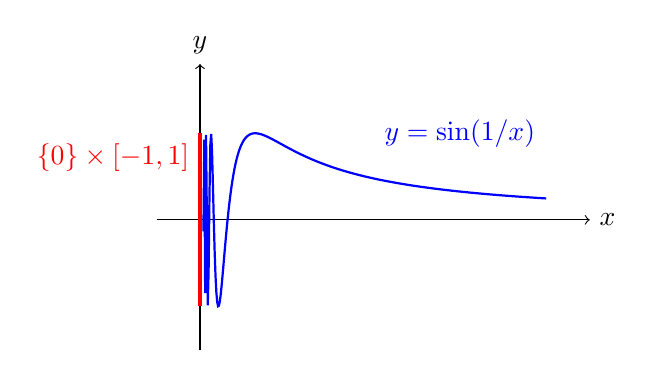
\begin{tikzpicture}[scale=1.1]
    \draw[->] (-0.5,0) -- (4.5,0) node[right] {$x$};
    \draw[->] (0,-1.5) -- (0,1.8) node[above] {$y$};
    \draw[very thick,red] (0,-1) -- (0,1) node[below left] {$\{0\} \times [-1, 1]$};
    \draw[domain=0.04:4,samples=400,variable=\x,blue,thick] 
        plot ({\x}, {sin((1/\x)*180/pi)});
    \node[blue] at (3,1) {$y = \sin(1/x)$};
\end{tikzpicture}
\end{center}

\textbf{2. Peine del topólogo:} En $\mathbb{R}^2$, consideremos:
\[
    P = ([0, 1] \times \{0\}) \cup \left(\bigcup_{n=1}^\infty \left\{\frac{1}{n}\right\} \times [0, 1]\right).
\]
$P$ es arcoconexo. El espacio $Y = P \cup \{(0, 1)\}$ es conexo (pues $P \subset Y \subset \overline{P}$), pero \textbf{no es arcoconexo}, ya que el punto $(0, 1)$ no puede unirse por camino a ningún otro punto de $Y$.

\begin{center}
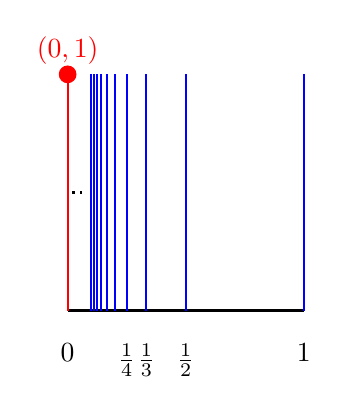
\begin{tikzpicture}[scale=3]
    \draw[thick] (0,0) -- (1,0);
    \foreach \n in {1, 2, 3, 4, 5, 6, 7, 8, 9, 10} {
        \draw[thick,blue] ({1/\n}, 0) -- ({1/\n}, 1);
    }
    \draw[thick,dotted] (0.02, 0.5) -- (0.08, 0.5);
    \draw[thick,red] (0,0) -- (0,1);
    \filldraw[red] (0,1) circle (1pt) node[above] {$(0, 1)$};
    \node at (1,-0.1) [below] {$1$};
    \node at (0.5,-0.1) [below] {$\frac{1}{2}$};
    \node at (0.333,-0.1) [below] {$\frac{1}{3}$};
    \node at (0.25,-0.1) [below] {$\frac{1}{4}$};
    \node at (0,-0.1) [below] {$0$};
\end{tikzpicture}
\end{center}
\end{ejem}

\section{Espacios localmente conexos y arcoconexos}

\begin{defi}
Un espacio topológico $X$ es \textbf{localmente conexo} (resp. \textbf{localmente arcoconexo}) si para todo punto $x \in X$ y todo abierto $U$ con $x \in U$, existe un abierto conexo (resp. arcoconexo) $V$ tal que $x \in V \subseteq U$.
\end{defi}

\begin{teo}
Un espacio $X$ es localmente conexo (resp. arcoconexo) si y solo si las componentes conexas (resp. arcoconexas) de cualquier abierto de $X$ son abiertas.
\end{teo}

\begin{cor}
Si $X$ es localmente conexo (o localmente arcoconexo), sus componentes conexas (o arcoconexas) son simultáneamente abiertas y cerradas.
\end{cor}

\begin{teo}
Si $X$ es un espacio conexo y localmente arcoconexo, entonces $X$ es arcoconexo. Además, en cualquier espacio localmente arcoconexo, las componentes conexas coinciden con las componentes arcoconexas.
\end{teo}

\begin{dem}
Sea $x_0 \in X$ y sea $Q_{x_0}$ la componente arcoconexa de $x_0$. Como $X$ es localmente arcoconexo, $Q_{x_0}$ es abierta. De igual modo, su complementario $X \setminus Q_{x_0} = \bigcup_{y \notin Q_{x_0}} Q_y$ es unión de abiertos, luego es abierto. Siendo $Q_{x_0} \ne \emptyset$ abierto y cerrado en el espacio conexo $X$, se concluye que $Q_{x_0} = X$, por lo que $X$ es arcoconexo.
\end{dem}

\section{Homotopía y grupo fundamental}

\begin{defi}
Sea $X$ un espacio topológico y $x \in X$. Un \textbf{lazo} con base en $x$ es un camino continuo $\gamma \colon [0, 1] \to X$ tal que $\gamma(0) = \gamma(1) = x$.
\end{defi}

\begin{defi}
Dos caminos $\gamma, \gamma' \colon [0, 1] \to X$ con los mismos extremos ($\gamma(0) = \gamma'(0)$ y $\gamma(1) = \gamma'(1)$) son \textbf{homótopos} (relativo a los extremos) si existe una aplicación continua:
\[
    H \colon [0, 1] \times [0, 1] \longrightarrow X
\]
tal que para todos $t, s \in [0, 1]$:
\begin{align*}
    H(t, 0) &= \gamma(t), \quad H(t, 1) = \gamma'(t), \\
    H(0, s) &= \gamma(0), \quad H(1, s) = \gamma(1).
\end{align*}
La relación de homotopía $\sim$ es una relación de equivalencia en la familia de lazos basados en $x$.
\end{defi}

\begin{center}
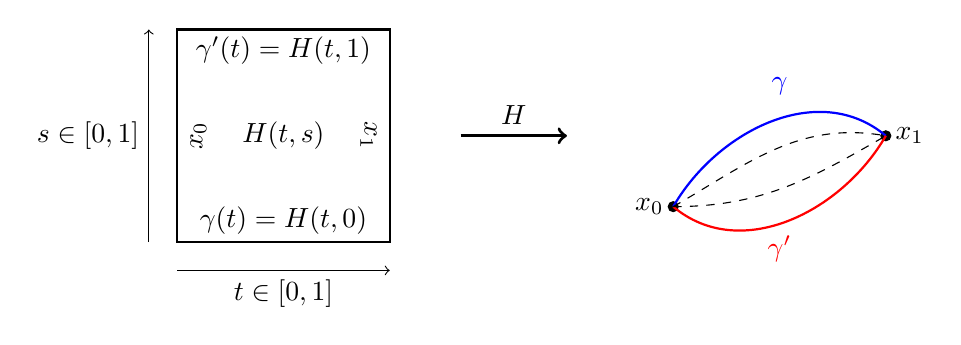
\begin{tikzpicture}[scale=0.9]
    \draw[thick] (0,0) rectangle (3,3);
    \draw[->] (0,-0.4) -- (3,-0.4) node[midway,below] {$t \in [0, 1]$};
    \draw[->] (-0.4,0) -- (-0.4,3) node[midway,left] {$s \in [0, 1]$};
    \node at (1.5,0.3) {$\gamma(t) = H(t, 0)$};
    \node at (1.5,2.7) {$\gamma'(t) = H(t, 1)$};
    \node at (0.3,1.5) [rotate=90] {$x_0$};
    \node at (2.7,1.5) [rotate=-90] {$x_1$};
    \node at (1.5,1.5) {$H(t, s)$};
    
    \draw[->,very thick] (4,1.5) -- (5.5,1.5) node[midway,above] {$H$};
    
    \begin{scope}[shift={(7,0.5)}]
        \filldraw[black] (0,0) circle (2pt) node[left] {$x_0$};
        \filldraw[black] (3,1) circle (2pt) node[right] {$x_1$};
        \draw[thick,blue] (0,0) to[out=60,in=140] (3,1);
        \draw[thick,red] (0,0) to[out=-40,in=-120] (3,1);
        \draw[dashed] (0,0) to[out=30,in=170] (3,1);
        \draw[dashed] (0,0) to[out=0,in=-150] (3,1);
        \node[blue] at (1.5,1.7) {$\gamma$};
        \node[red] at (1.5,-0.6) {$\gamma'$};
    \end{scope}
\end{tikzpicture}
\end{center}

\begin{defi}
El conjunto de clases de homotopía de lazos basados en $x$, dotado de la concatenación $[\gamma] \cdot [\gamma'] = [\gamma * \gamma']$, forma un grupo denominado el \textbf{grupo fundamental} de $X$ en el punto base $x$, denotado $\pi_1(X, x)$. El elemento neutro es la clase del lazo constante $e_x(t) = x$, y el inverso de $[\gamma]$ es la clase del lazo recorrido en sentido inverso $\gamma^{-1}(t) = \gamma(1 - t)$.
\end{defi}

\begin{prop}
Si $X$ es arcoconexo, para cualesquiera $x, x' \in X$ se verifica $\pi_1(X, x) \cong \pi_1(X, x')$, por lo que se escribe $\pi_1(X)$.
\end{prop}

\begin{ejem}
\begin{itemize}
    \item $\pi_1(\mathbb{R}^n) = \{0\}$.
    \item $\pi_1(\mathbb{R}^2 \setminus \{(0, 0)\}) \cong \pi_1(S^1) \cong \mathbb{Z}$.
    \item $\pi_1(S^2) = \{0\}$.
    \item $\pi_1(\mathbb{T}^2) \cong \mathbb{Z} \times \mathbb{Z}$ para el toro 2-dimensional.
\end{itemize}
\end{ejem}

\begin{defi}
Un espacio topológico $X$ es \textbf{simplemente conexo} si es arcoconexo y su grupo fundamental es trivial: $\pi_1(X) = \{0\}$.
\end{defi}

\section{Espacios irreducibles}

\begin{defi}
Un espacio topológico $X$ es \textbf{irreducible} si no se puede expresar como unión de dos subconjuntos cerrados propios:
\[
    X = C_1 \cup C_2 \text{ con } C_1, C_2 \text{ cerrados} \Rightarrow X = C_1 \quad \text{o} \quad X = C_2.
\]
\end{defi}

\begin{prop}
En cualquier espacio topológico $X$, son equivalentes:
\begin{enumerate}
    \item[\textbf{1)}] $X$ es irreducible.
    \item[\textbf{2)}] Dos abiertos no vacíos cualesquiera se cortan siempre: $U, V \in \mc T \setminus \{\emptyset\} \Rightarrow U \cap V \ne \emptyset$.
    \item[\textbf{3)}] Todo abierto no vacío $U$ es denso en $X$: $\overline{U} = X$.
\end{enumerate}
\end{prop}

\begin{dem}
\begin{itemize}
    \item[\textbf{1 $\iff$ 2:}] Sean $U, V$ abiertos. $(X \setminus U) \cup (X \setminus V) = X \setminus (U \cap V)$. Por definición de irreducibilidad, esta unión de cerrados es todo $X \iff X \setminus U = X$ o $X \setminus V = X$, es decir, $U \cap V = \emptyset \iff U = \emptyset$ o $V = \emptyset$.
    \item[\textbf{2 $\iff$ 3:}] $U$ es denso $\iff$ todo abierto no vacío corta a $U$.
\end{itemize}
\end{dem}

\begin{obs}
\begin{itemize}
    \item Todo espacio irreducible es conexo. El recíproco es falso: $\mathbb{R}^2$ euclídeo es conexo pero no es irreducible (por ejemplo, dos abiertos disjuntos no se cortan).
    \item Un espacio de Hausdorff ($T_2$) es irreducible si y solo si consta de a lo sumo un punto.
    \item La topología de Zariski en geometría algebraica da lugar a espacios irreducibles estándar.
\end{itemize}
\end{obs}

\begin{ejem}
\begin{itemize}
    \item En $(\mathbb{R}, \mc T_{\text{kol}})$ con $\mc T_{\text{kol}} = \{(a, \infty) \mid a \in \mathbb{R}\} \cup \{\emptyset, \mathbb{R}\}$, cualesquiera dos abiertos $(a, \infty) \cap (b, \infty) = (\max\{a, b\}, \infty) \ne \emptyset$, luego $(\mathbb{R}, \mc T_{\text{kol}})$ es irreducible.
    \item La unión de los dos ejes coordenados en el plano afín $X = \{(x, y) \mid xy = 0\} = C_1 \cup C_2$ no es irreducible, siendo sus componentes irreducibles las rectas $C_1 = \{y = 0\}$ y $C_2 = \{x = 0\}$.
\end{itemize}

\begin{center}
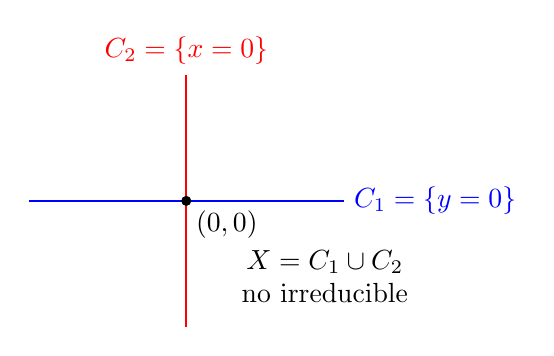
\begin{tikzpicture}[scale=0.8]
    \draw[thick,blue] (-2.5,0) -- (2.5,0) node[right] {$C_1 = \{y=0\}$};
    \draw[thick,red] (0,-2) -- (0,2) node[above] {$C_2 = \{x=0\}$};
    \filldraw[black] (0,0) circle (2pt) node[below right] {$(0, 0)$};
    \node at (2.2,-1.2) [align=center] {$X = C_1 \cup C_2$ \\ no irreducible};
\end{tikzpicture}
\end{center}
\end{ejem}


































\chapter{Espacios topol\'ogicos compactos}Sea \(X\) un espacio topológico.

\section{Espacios Compactos y Subespacios}

\begin{defi}
Sea \(X\) un espacio topológico:
\begin{itemize}
    \item Un \textbf{recubrimiento abierto} de \(X\) es una familia de abiertos \(\{U_i\}_{i \in I}\) de \(X\) tal que \(X = \bigcup_{i \in I} U_i\).
    \item Un \textbf{subrecubrimiento} de \(\{U_i\}_{i \in I}\) es una subfamilia \(\{U_j\}_{j \in J}\) con \(J \subseteq I\) tal que \(X = \bigcup_{j \in J} U_j\).
    \item Un \textbf{refinamiento} de \(\{U_i\}_{i \in I}\) es un recubrimiento abierto \(\{V_j\}_{j \in J}\) tal que para cada \(j \in J\) existe \(i(j) \in I\) con \(V_j \subseteq U_{i(j)}\).
\end{itemize}
\end{defi}

\begin{defi}
Un espacio topológico \(X\) es \textbf{compacto} si todo recubrimiento abierto de \(X\) admite un subrecubrimiento finito:
\[
    X = \bigcup_{i \in I} U_i \Rightarrow \exists i_1, \ldots, i_r \in I \quad \text{tal que} \quad X = \bigcup_{j=1}^r U_{i_j}.
\]
Un subespacio \(Y \subseteq X\) es compacto si lo es con su topología relativa; equivalentemente, para toda familia de abiertos \(\{U_i\}_{i \in I}\) en \(X\) tal que \(Y \subseteq \bigcup_{i \in I} U_i\), existen \(i_1, \ldots, i_r \in I\) tales que \(Y \subseteq \bigcup_{j=1}^r U_{i_j}\).
\end{defi}

\begin{ejem}
\((\mathbb{R}, \mc T_d)\) no es compacto: el recubrimiento \(\mathbb{R} = \bigcup_{n \in \mathbb{Z}} (n - 1, n + 1)\) no admite ningún subrecubrimiento finito.
\end{ejem}

\begin{prop}
Sea \(X\) un espacio topológico compacto y sea \(Y \subseteq X\) un subconjunto cerrado. Entonces \(Y\) es compacto.
\end{prop}

\begin{dem}
Sea \(\{U_i\}_{i \in I}\) una familia de abiertos de \(X\) que recubren a \(Y\), es decir, \(Y \subseteq \bigcup_{i \in I} U_i\). Como \(Y\) es cerrado en \(X\), su complementario \(V \coloneqq X \setminus Y\) es abierto en \(X\). Entonces la colección \(\{U_i\}_{i \in I} \cup \{V\}\) constituye un recubrimiento abierto de todo el espacio \(X\). Por ser \(X\) compacto, existen índices \(i_1, \ldots, i_r \in I\) tales que:
\[
    X = U_{i_1} \cup \ldots \cup U_{i_r} \cup V.
\]
Intersecando con \(Y\) (y observando que \(V \cap Y = \emptyset\)), obtenemos:
\[
    Y \subseteq U_{i_1} \cup \ldots \cup U_{i_r}.
\]
Por consiguiente, \(Y\) es compacto.
\end{dem}

\begin{prop}
Sea \(X\) un espacio topológico de Hausdorff (\(T_2\)) e \(Y \subseteq X\) un subespacio compacto. Para todo punto \(x \notin Y\), existen abiertos disjuntos \(U_x, U_Y \subseteq X\) tales que \(x \in U_x\) e \(Y \subseteq U_Y\). En particular, \(Y\) es cerrado en \(X\).
\end{prop}

\begin{dem}
Sea \(x \notin Y\). Para cada \(y \in Y\), como \(x \ne y\) y el espacio \(X\) es separado (\(T_2\)), existen abiertos disjuntos \(U_x^y \ni x\) y \(U_y \ni y\) tales que \(U_x^y \cap U_y = \emptyset\). La familia \(\{U_y\}_{y \in Y}\) es un recubrimiento abierto del subespacio compacto \(Y\). Por compacidad, existen \(y_1, \ldots, y_r \in Y\) tales que:
\[
    Y \subseteq U_Y \coloneqq U_{y_1} \cup \ldots \cup U_{y_r}.
\]
Definimos ahora el conjunto:
\[
    U_x \coloneqq \bigcap_{j=1}^r U_x^{y_j},
\]
el cual es abierto por ser intersección finita de abiertos y contiene a \(x\). Comprobamos que son disjuntos:
\[
    U_x \cap U_Y = U_x \cap \left(\bigcup_{j=1}^r U_{y_j}\right) = \bigcup_{j=1}^r (U_x \cap U_{y_j}) \subseteq \bigcup_{j=1}^r (U_x^{y_j} \cap U_{y_j}) = \emptyset.
\]
Para probar que \(Y\) es cerrado, observamos que para todo punto \(x \notin Y\) hemos encontrado un abierto \(U_x\) tal que \(x \in U_x \subseteq X \setminus Y\). Por consiguiente, \(X \setminus Y\) es abierto en \(X\), de donde \(Y\) es cerrado.
\end{dem}

\begin{teo}
\begin{enumerate}
    \item[\textbf{a)}] Si \(X\) es compacto e \(Y \subseteq X\) es cerrado, entonces \(Y\) es compacto.
    \item[\textbf{b)}] Si \(X\) es de Hausdorff (\(T_2\)) e \(Y \subseteq X\) es compacto, entonces \(Y\) es cerrado.
    \item[\textbf{c)}] Si \(X\) es compacto y \(T_2\), un subespacio \(Y \subseteq X\) es compacto si y solo si \(Y\) es cerrado.
\end{enumerate}
\end{teo}

\begin{prop}
Sea \(f \colon X \to Y\) una aplicación continua. Si \(X\) es compacto, entonces su imagen \(\operatorname{Im}(f) = f(X) \subseteq Y\) es un subespacio compacto de \(Y\).
\end{prop}

\begin{dem}
Sea \(\{V_i\}_{i \in I}\) un recubrimiento abierto de \(\operatorname{Im}(f)\) en \(Y\): \(\operatorname{Im}(f) \subseteq \bigcup_{i \in I} V_i\). Aplicando la anti-imagen \(f^{-1}\):
\[
    X = f^{-1}(\operatorname{Im}(f)) \subseteq f^{-1}\left(\bigcup_{i \in I} V_i\right) = \bigcup_{i \in I} f^{-1}(V_i).
\]
Al ser \(f\) continua, cada \(f^{-1}(V_i)\) es un abierto de \(X\). Como \(X\) es compacto, existen \(i_1, \ldots, i_r \in I\) tales que:
\[
    X = \bigcup_{j=1}^r f^{-1}(V_{i_j}).
\]
Aplicando la imagen directa:
\[
    \operatorname{Im}(f) = f(X) = f\left(\bigcup_{j=1}^r f^{-1}(V_{i_j})\right) = \bigcup_{j=1}^r f(f^{-1}(V_{i_j})) \subseteq \bigcup_{j=1}^r V_{i_j}.
\]
Por consiguiente, \(\operatorname{Im}(f)\) es compacto.
\end{dem}

\begin{cor}
\(\mathbb{R}^n\) no es compacto para ningún \(n \ge 1\).
\end{cor}

\begin{dem}
La proyección canónica sobre la primera coordenada \(\pi_1 \colon \mathbb{R}^n \to \mathbb{R}\) es continua y sobreyectiva. Si \(\mathbb{R}^n\) fuese compacto, su imagen continua \(\operatorname{Im}(\pi_1) = \mathbb{R}\) sería compacta, lo cual es falso.
\end{dem}

\section{Compacidad en \(\mathbb{R}\) y \(\mathbb{R}^n\)}

\begin{prop}
Para cualesquiera \(a < b \in \mathbb{R}\), el intervalo cerrado \([a, b]\) es compacto en \((\mathbb{R}, \mc T_d)\).
\end{prop}

\begin{dem}
Sea \(\{U_i\}_{i \in I}\) una familia de abiertos de \(\mathbb{R}\) tal que \([a, b] \subseteq \bigcup_{i \in I} U_i\). Como \(a \in [a, b]\), existe algún \(i_0 \in I\) con \(a \in U_{i_0}\). Por apertura de \(U_{i_0}\), existe \(\varepsilon > 0\) tal que \([a, a + \varepsilon) \subseteq U_{i_0}\). Consideramos el conjunto:
\[
    C \coloneqq \{x \in [a, b] \mid [a, x] \text{ está recubierto por un número finito de abiertos } U_i\}.
\]
El conjunto \(C\) es no vacío (pues \(a \in C\) y \([a, a + \varepsilon) \subseteq C\)) y está acotado superiormente por \(b\). Por el axioma del supremo de los números reales, existe \(c \coloneqq \sup(C) \le b\).

Veamos primero que \(c \in C\). Como \(c \in [a, b]\), existe \(j_0 \in I\) con \(c \in U_{j_0}\). Al ser \(U_{j_0}\) abierto, existe \(\delta > 0\) tal que \((c - \delta, c + \delta) \subseteq U_{j_0}\). Al ser \(c = \sup(C)\), existe algún elemento \(x \in C\) con \(c - \delta < x \le c\). Por pertenecer a \(C\), \([a, x]\) está recubierto por un número finito de abiertos \(U_{i_1}, \ldots, U_{i_m}\). Como \([x, c] \subseteq (c - \delta, c + \delta) \subseteq U_{j_0}\), se deduce que:
\[
    [a, c] = [a, x] \cup [x, c] \subseteq U_{i_1} \cup \ldots \cup U_{i_m} \cup U_{j_0},
\]
lo cual demuestra que \([a, c]\) admite un subrecubrimiento finito, es decir, \(c \in C\).

Veamos ahora que \(c = b\). Si fuera \(c < b\), tomando \(\delta' \coloneqq \min\{\delta/2, b - c\} > 0\), el intervalo \([c, c + \delta'] \subseteq U_{j_0}\), con lo cual \([a, c + \delta'] = [a, c] \cup [c, c + \delta']\) admitiría un recubrimiento finito, implicando que \(c + \delta' \in C\). Pero \(c + \delta' > c = \sup(C)\), contradicción. Así pues, \(c = b \in C\), concluyendo que \([a, b]\) es compacto.
\end{dem}

\begin{cor}
En \((\mathbb{R}, \mc T_d)\), un subespacio \(Y \subseteq \mathbb{R}\) es compacto si y solo si es cerrado y acotado.
\end{cor}

\begin{dem}
\begin{itemize}
    \item[(\(\Rightarrow\))] Sea \(Y \subseteq \mathbb{R}\) compacto. Puesto que \((\mathbb{R}, \mc T_d)\) es de Hausdorff (\(T_2\)), por la Propiedad 1.2 \(Y\) es cerrado. Por otra parte, \(\mathbb{R} = \bigcup_{n \in \mathbb{N}} B_d(0, n) = \bigcup_{n \in \mathbb{N}} (-n, n)\), luego \(Y \subseteq \bigcup_{n \in \mathbb{N}} B_d(0, n)\). Al ser \(Y\) compacto, existen \(n_1, \ldots, n_r \in \mathbb{N}\) tales que:
    \[
        Y \subseteq \bigcup_{j=1}^r B_d(0, n_j) = B_d(0, M) = (-M, M),
    \]
    donde \(M \coloneqq \max\{n_1, \ldots, n_r\}\). En consecuencia, \(Y\) es acotado.
    \item[(\(\Leftarrow\))] Supongamos que \(Y\) es cerrado y acotado. Por ser acotado, existen \(a, b \in \mathbb{R}\) tales que \(Y \subseteq [a, b]\). Como \([a, b]\) es compacto en \(\mathbb{R}\) e \(Y\) es un subconjunto cerrado de \([a, b]\), por la Propiedad 1.1 deducimos que \(Y\) es compacto.
\end{itemize}
\end{dem}

\subsection{El lema del entorno tubular y Teorema de Tychonoff}

\begin{lema}[Lema del tubo o del entorno tubular]
Sean \(X, Y\) espacios topológicos con \(Y\) compacto. Sea \(x_0 \in X\) y sea \(U \subseteq X \times Y\) un abierto tal que \(\{x_0\} \times Y \subseteq U\). Entonces existe un abierto \(W_{x_0} \subseteq X\) con \(x_0 \in W_{x_0}\) tal que:
\[
    W_{x_0} \times Y \subseteq U.
\]
\end{lema}

\begin{dem}
Sea \(y \in Y\). El punto \((x_0, y) \in \{x_0\} \times Y \subseteq U\). Como los productos de abiertos forman una base de la topología de \(X \times Y\), existen abiertos \(U_{x_0}^y \subseteq X\) y \(V_y \subseteq Y\) tales que:
\[
    (x_0, y) \in U_{x_0}^y \times V_y \subseteq U.
\]
La colección \(\{V_y\}_{y \in Y}\) es un recubrimiento por abiertos de \(Y\). Siendo \(Y\) compacto, existen puntos \(y_1, \ldots, y_r \in Y\) tales que \(Y = \bigcup_{j=1}^r V_{y_j}\). Definimos:
\[
    W_{x_0} \coloneqq \bigcap_{j=1}^r U_{x_0}^{y_j}.
\]
\(W_{x_0}\) es abierto por ser intersección finita de abiertos, y contiene a \(x_0\) porque cada \(U_{x_0}^{y_j}\) lo contiene. Comprobemos que \(W_{x_0} \times Y \subseteq U\): sea \((x, y) \in W_{x_0} \times Y\). Como \(y \in Y = \bigcup_{j=1}^r V_{y_j}\), existe algún \(j \in \{1, \ldots, r\}\) tal que \(y \in V_{y_j}\). Puesto que \(x \in W_{x_0} \subseteq U_{x_0}^{y_j}\), se sigue que:
\[
    (x, y) \in U_{x_0}^{y_j} \times V_{y_j} \subseteq U.
\]
Por lo tanto, \(W_{x_0} \times Y \subseteq U\).
\end{dem}

\begin{center}
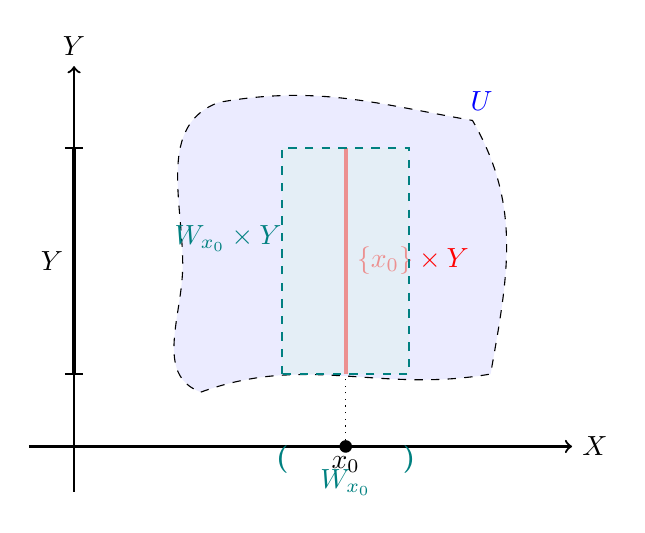
\begin{tikzpicture}[scale=1.15]
    % Ejes coordenados X e Y
    \draw[->,thick] (-0.5,0) -- (5.5,0) node[right] {\(X\)};
    \draw[->,thick] (0,-0.5) -- (0,4.2) node[above] {\(Y\)};
    
    % Abierto U grande que envuelve la fibra
    \draw[dashed,fill=blue!8] 
        (1.4,0.6) to[out=20,in=190] (4.6,0.8) 
        to[out=80,in=-60] (4.4,3.6) 
        to[out=170,in=10] (1.6,3.8) 
        to[out=200,in=90] (1.2,2)
        to[out=-90,in=160] cycle;
    \node[blue] at (4.5,3.6) [above] {\(U\)};
    
    % Fibra vertical {x_0} x Y
    \draw[line width=1.5pt,red] (3,0.8) -- (3,3.3) node[midway,right] {\(\{x_0\} \times Y\)};
    \filldraw[black] (3,0) circle (1.8pt) node[below] {\(x_0\)};
    \draw[dotted] (3,0) -- (3,0.8);
    
    % Paréntesis del abierto W en el eje X
    \draw[thick,teal] (2.3,-0.15) node {\textbf{(}} (3.7,-0.15) node {\textbf{)}};
    \node[teal] at (3,-0.4) {\(W_{x_0}\)};
    
    % Rectángulo tubular W x Y
    \draw[thick,teal,dashed,fill=teal!12,fill opacity=0.6] (2.3,0.8) rectangle (3.7,3.3);
    \node[teal] at (2.4,2.3) [left] {\(W_{x_0} \times Y\)};
    
    % Proyecciones de Y en el eje vertical
    \draw[thick] (-0.1,0.8) -- (0.1,0.8);
    \draw[thick] (-0.1,3.3) -- (0.1,3.3);
    \draw[very thick] (0,0.8) -- (0,3.3) node[midway,left] {\(Y\)};
\end{tikzpicture}
\qquad
\begin{tikzpicture}[scale=0.9]
    \draw[->,thick] (-2.2,0) -- (2.2,0) node[right] {\(x\)};
    \draw[->,thick] (0,-2.2) -- (0,2.2) node[above] {\(y\)};
    
    % Hiperbola xy=1
    \draw[thick,blue,domain=0.45:2,samples=60] plot (\x, {1/\x});
    \draw[thick,blue,domain=-2:-0.45,samples=60] plot (\x, {1/\x});
    \draw[very thick,red] (0,-2) -- (0,2) node[left,pos=0.8] {\(\{0\} \times \mathbb{R}\)};
    
    \node at (0,-2.7) [align=center] {Contraejemplo: en \(\mathbb{R} \times \mathbb{R}\) con \(Y=\mathbb{R}\) no compacto, \\ \(\{0\} \times \mathbb{R} \subset (\text{hipérbola})^c\) no admite tubo \(W \times \mathbb{R}\)};
\end{tikzpicture}
\end{center}

\begin{obs}
La hipótesis de que \(Y\) sea compacto es fundamental. En \(\mathbb{R}^2\), el complementario de la hipérbola \(U = \mathbb{R}^2 \setminus \{(x, y) \mid xy = 1\}\) contiene a la recta \(\{0\} \times \mathbb{R}\), pero ningún entorno \(W \times \mathbb{R}\) cabe en \(U\) porque las ramas de la hipérbola se acercan asintóticamente a los ejes.
\end{obs}

\begin{teo}[Teorema de Tychonoff]
Sean \(\{X_i\}_{i \in I}\) espacios topológicos. El producto \(\prod_{i \in I} X_i\) es compacto si y solo si cada \(X_i\) es compacto.
\end{teo}

\begin{dem}
\begin{itemize}
    \item[(\(\Rightarrow\))] Para cada \(j \in I\), la proyección canónica \(\pi_j \colon \prod_{i \in I} X_i \to X_j\) es continua y sobreyectiva. Como la imagen continua de un compacto es compacta, cada \(X_j = \pi_j(\prod X_i)\) es compacto.
    \item[(\(\Leftarrow\))] Demostraremos el caso para el producto de dos espacios compactos \(X \times Y\) (el caso finito general se sigue por inducción):
    
    Sea \(\{U_i\}_{i \in I}\) un recubrimiento abierto de \(X \times Y\). Fijemos \(x \in X\). El subespacio \(\{x\} \times Y \cong Y\) es compacto, luego está cubierto por un número finito de abiertos:
    \[
        \{x\} \times Y \subseteq U_{i_1}^x \cup \ldots \cup U_{i_r}^x =: \mathcal{U}^x.
    \]
    Por el lema del entorno tubular, existe un abierto \(W_x \subseteq X\) con \(x \in W_x\) tal que \(W_x \times Y \subseteq \mathcal{U}^x\).
    
    La familia \(\{W_x\}_{x \in X}\) es un recubrimiento abierto de \(X\). Como \(X\) es compacto, existen puntos \(x_1, \ldots, x_m \in X\) tales que:
    \[
        X = W_{x_1} \cup \ldots \cup W_{x_m}.
    \]
    Por consiguiente:
    \[
        X \times Y = \bigcup_{k=1}^m (W_{x_k} \times Y) \subseteq \bigcup_{k=1}^m \mathcal{U}^{x_k}.
    \]
    Puesto que cada \(\mathcal{U}^{x_k}\) es unión finita de abiertos \(U_i\), hemos obtenido un subrecubrimiento finito de \(X \times Y\).
\end{itemize}
\end{dem}

\begin{cor}[Teorema de Heine-Borel en \(\mathbb{R}^n\)]
Un subconjunto \(Y \subseteq \mathbb{R}^n\) es compacto si y solo si es cerrado y acotado.
\end{cor}

\begin{dem}
\begin{itemize}
    \item[(\(\Rightarrow\))] Si \(Y \subseteq \mathbb{R}^n\) es compacto, al ser \(\mathbb{R}^n\) de Hausdorff, \(Y\) es cerrado. Por otra parte, \(\mathbb{R}^n = \bigcup_{m \in \mathbb{N}} B_d(0, m)\), luego por compacidad \(Y \subseteq B_d(0, M)\) para algún \(M\), de modo que \(Y\) es acotado.
    \item[(\(\Leftarrow\))] Si \(Y\) es acotado, existen intervalos compactos \([a_i, b_i] \subset \mathbb{R}\) tales que \(Y \subseteq [a_1, b_1] \times \ldots \times [a_n, b_n]\). Por el Teorema de Tychonoff, este producto cartesiano de compactos es compacto. Al ser \(Y\) cerrado en \(\mathbb{R}^n\), es cerrado dentro de dicho producto compacto, y por la Propiedad 1.1, \(Y\) es compacto.
\end{itemize}
\end{dem}

\section{Compacidad por Familias de Cerrados (PIF)}

\begin{defi}
Una familia de subconjuntos cerrados \(\{C_i\}_{i \in I}\) de un espacio \(X\) tiene la \textbf{propiedad de la intersección finita (PIF)} si para toda subfamilia finita \(\{i_1, \ldots, i_r\} \subseteq I\), su intersección es no vacía:
\[
    \bigcap_{j=1}^r C_{i_j} \ne \emptyset.
\]
\end{defi}

\begin{prop}
Un espacio topológico \(X\) es compacto si y solo si toda familia de cerrados \(\{C_i\}_{i \in I}\) con la PIF verifica \(\bigcap_{i \in I} C_i \ne \emptyset\).
\end{prop}

\begin{dem}
\begin{itemize}
    \item[(\(\Rightarrow\))] Sea \(\{C_i\}_{i \in I}\) una familia de cerrados con la PIF. Supongamos por reducción al absurdo que \(\bigcap_{i \in I} C_i = \emptyset\). Tomando complementarios, los conjuntos \(U_i \coloneqq X \setminus C_i\) son abiertos y:
    \[
        \bigcup_{i \in I} U_i = \bigcup_{i \in I} (X \setminus C_i) = X \setminus \left(\bigcap_{i \in I} C_i\right) = X \setminus \emptyset = X.
    \]
    Por ser \(X\) compacto, existen índices \(i_1, \ldots, i_r \in I\) tales que \(X = U_{i_1} \cup \ldots \cup U_{i_r}\). Tomando complementarios de nuevo:
    \[
        \emptyset = X \setminus X = X \setminus (U_{i_1} \cup \ldots \cup U_{i_r}) = C_{i_1} \cap \ldots \cap C_{i_r},
    \]
    lo cual contradice que la familia \(\{C_i\}\) cumple la PIF. Por tanto, \(\bigcap_{i \in I} C_i \ne \emptyset\).
    \item[(\(\Leftarrow\))] Sea \(\{U_i\}_{i \in I}\) un recubrimiento abierto de \(X\): \(\bigcup_{i \in I} U_i = X\). Consideremos la familia de cerrados \(C_i \coloneqq X \setminus U_i\). Entonces \(\bigcap_{i \in I} C_i = X \setminus \bigcup_{i \in I} U_i = \emptyset\). Por hipótesis, la familia \(\{C_i\}\) no puede verificar la PIF, lo que significa que existe una subfamilia finita con \(C_{i_1} \cap \ldots \cap C_{i_r} = \emptyset\). Tomando complementarios, \(U_{i_1} \cup \ldots \cup U_{i_r} = X\), probando que \(X\) es compacto.
\end{itemize}
\end{dem}

\begin{cor}[Teorema de Cantor para cadenas encajadas]
Sea \(X\) un espacio compacto y sea \(\{C_n\}_{n \in \mathbb{N}}\) una cadena descendente de cerrados no vacíos (\(C_1 \supseteq C_2 \supseteq \ldots \supseteq C_n \supseteq \ldots\)). Entonces:
\[
    \bigcap_{n=1}^\infty C_n \ne \emptyset.
\]
\end{cor}

\begin{dem}
Para cualquier subcolección finita \(\{C_{n_1}, \ldots, C_{n_r}\}\), si \(m \coloneqq \max\{n_1, \ldots, n_r\}\), entonces \(\bigcap_{j=1}^r C_{n_j} = C_m \ne \emptyset\). Así, la cadena cumple la PIF, y por compacidad de \(X\), la intersección total es no vacía.
\end{dem}

\begin{lema}
Sea \(X\) un espacio de Hausdorff (\(T_2\)) sin puntos aislados. Si \(U \subseteq X\) es un abierto no vacío y \(x \in X\), entonces existe un abierto no vacío \(V \subseteq X\) tal que \(V \subseteq U\) y \(x \notin \overline{V}\).
\end{lema}

\begin{dem}
\begin{itemize}
    \item Si \(x \notin U\), como \(U\) es no vacío existe \(y \in U\). Al ser \(X\) separado, existen abiertos disjuntos \(U_x \ni x\) y \(U_y \ni y\). Tomando \(V \coloneqq U \cap U_y\), se tiene \(V \subseteq U\) y como \(V \cap U_x = \emptyset\), \(x \notin \overline{V}\).
    \item Si \(x \in U\), como \(X\) no tiene puntos aislados \(\{x\}\) no es abierto, luego existe \(y \in U\) con \(y \ne x\). Por ser \(X\) de Hausdorff, existen abiertos disjuntos \(U_x \ni x\) y \(U_y \ni y\). Definiendo \(V \coloneqq U \cap U_y\), \(V\) es un abierto no vacío contenido en \(U\), y como \(V \cap U_x = \emptyset\), \(x \notin \overline{V}\).
\end{itemize}
\end{dem}

\begin{prop}
Todo espacio métrico compacto, de Hausdorff y sin puntos aislados es no contable (no numerable).
\end{prop}

\begin{dem}
Supongamos por contradicción que \(X\) es numerable, es decir, existe una biyección \(f \colon \mathbb{N} \to X\) con \(X = \{x_1, x_2, \ldots, x_n, \ldots\}\). 

Tomamos \(U_1 \coloneqq X\). Por el Lema 2.2, existe un abierto no vacío \(V_1\) tal que \(V_1 \subseteq U_1\) y \(x_1 \notin \overline{V}_1\). Tomamos ahora \(U_2 \coloneqq V_1\); aplicando nuevamente el lema, existe un abierto no vacío \(V_2\) con \(V_2 \subseteq U_2 = V_1\) tal que \(x_2 \notin \overline{V}_2\).

Reiterando el proceso, obtenemos una sucesión de abiertos encajados \(\ldots \subseteq V_n \subseteq V_{n-1} \subseteq \ldots \subseteq V_1\) tales que para cada \(n \in \mathbb{N}\), \(x_n \notin \overline{V}_n\). Sus clausuras forman una cadena descendente de cerrados no vacíos encajados:
\[
    \overline{V}_1 \supseteq \overline{V}_2 \supseteq \ldots \supseteq \overline{V}_n \supseteq \ldots
\]
Por ser \(X\) compacto, por el corlario 3.1 la intersección es no vacía: existe algún punto \(x \in \bigcap_{n=1}^\infty \overline{V}_n\). Pero como \(X = \{x_n\}_{n \in \mathbb{N}}\), debe ser \(x = x_m\) para algún \(m \in \mathbb{N}\). Sin embargo, por construcción \(x_m \notin \overline{V}_m\), contradiciendo que \(x \in \bigcap \overline{V}_n\). Por tanto, \(X\) es no numerable.
\end{dem}

\section{Espacios Localmente Compactos y Compactificación}

\begin{defi}
Un espacio topológico \(X\) es \textbf{localmente compacto} si para todo punto \(x \in X\) existe un entorno compacto \(K \subseteq X\) de \(x\) (es decir, \(x \in K^\circ \subseteq K\)).
\end{defi}

\begin{teo}
Si \(X\) es de Hausdorff (\(T_2\)), son equivalentes:
\begin{enumerate}
    \item[\textbf{1)}] \(X\) es localmente compacto.
    \item[\textbf{2)}] Para todo abierto \(U \subseteq X\) y todo punto \(x \in U\), existe un abierto \(V\) tal que \(x \in V \subseteq \overline{V} \subseteq U\), con \(\overline{V}\) compacto.
\end{enumerate}
\end{teo}

\begin{dem}
\begin{itemize}
    \item[\textbf{2 \(\Rightarrow\) 1:}] Basta tomar \(U = X\).
    \item[\textbf{1 \(\Rightarrow\) 2:}] Sea \(x \in U\) abierto. Como \(X\) es localmente compacto, existe un entorno compacto \(K\) con \(x \in K^\circ \subseteq K\). Por ser \(X\) de Hausdorff, \(K\) es cerrado. El conjunto \(A \coloneqq K \setminus U = K \cap (X \setminus U)\) es cerrado dentro del compacto \(K\), luego \(A\) es compacto. Además, \(x \notin A\) porque \(x \in U\). Por la Propiedad 1.2, existen abiertos disjuntos \(V_x, V_A \subseteq X\) tales que \(x \in V_x\) y \(A \subseteq V_A\).
    
    Definimos \(V \coloneqq V_x \cap K^\circ\), que es abierto y contiene a \(x\). Como \(V \subseteq K^\circ \subseteq K\), se tiene \(\overline{V} \subseteq K\), de modo que \(\overline{V}\) es compacto por ser cerrado dentro de \(K\). Finalmente, comprobemos que \(\overline{V} \subseteq U\): si existiera \(y \in \overline{V} \setminus U\), entonces \(y \in K \setminus U = A \subseteq V_A\); pero como \(y \in \overline{V}\) y \(V_A\) es un entorno abierto de \(y\), debería ser \(V_A \cap V \ne \emptyset\), lo cual es imposible puesto que \(V_A \cap V \subseteq V_A \cap V_x = \emptyset\). Así, \(\overline{V} \subseteq U\).
\end{itemize}
\end{dem}

\begin{cor}
Si \(X\) es localmente compacto, todo subespacio cerrado \(C \subseteq X\) es localmente compacto.
\end{cor}

\begin{dem}
Sea \(x \in C\). Como \(X\) es localmente compacto, existe un compacto \(K \subseteq X\) tal que \(x \in K^\circ \subseteq K\). Entonces \(K \cap C\) es un subespacio cerrado dentro del compacto \(K\), luego \(K \cap C\) es compacto en \(C\). Además, \(x \in K^\circ \cap C \subseteq K \cap C\), y \(K^\circ \cap C\) es abierto en \(C\). Así, \(K \cap C\) es un entorno compacto de \(x\) en \(C\).
\end{dem}

\begin{cor}
Si \(X\) es localmente compacto y de Hausdorff, todo subespacio abierto \(U \subseteq X\) es localmente compacto.
\end{cor}

\begin{dem}
Para cualquier \(x \in U\), por el Teorema 4.1 existe un abierto \(V\) tal que \(x \in V \subseteq \overline{V} \subseteq U\) con \(\overline{V}\) compacto. Entonces \(\overline{V}\) es un entorno compacto de \(x\) en \(U\).
\end{dem}

\subsection{Compactificación de Alexandroff}

\begin{defi}
Sea \(X\) un espacio de Hausdorff localmente compacto que no es compacto. Se define \(X^* \coloneqq X \cup \{\infty\}\) con la topología formada por:
\begin{itemize}
    \item Los abiertos de \(X\): \(U \subseteq X\) con \(U \in \mc T_X\).
    \item Los conjuntos de la forma \(X^* \setminus K\), donde \(K \subseteq X\) es compacto.
\end{itemize}
\end{defi}

\begin{teo}
\(X^*\) es un espacio topológico compacto y de Hausdorff. Además, la inclusión natural \(i \colon X \hookrightarrow X^*\) es una inmersión abierta y \(X\) es denso en \(X^*\).
\end{teo}

\begin{dem}
\begin{enumerate}
    \item[\textbf{1)}] \textbf{Inclusión abierta:} \(\operatorname{Im}(i) = X = X^* \setminus \{\infty\}\). Como el conjunto vacío \(\emptyset\) es compacto, \(X^* \setminus \emptyset = X^*\) es abierto, y para \(V \in \mc T_{X^*}\), \(i^{-1}(V) = V \cap X \in \mc T_X\), de modo que \(i\) es un homeomorfismo sobre su imagen abierta \(X\).
    \item[\textbf{2)}] \textbf{\(X^*\) es de Hausdorff (\(T_2\)):} Sean \(z \ne z' \in X^*\):
    \begin{itemize}
        \item Si \(z, z' \in X\), como \(X\) es \(T_2\) existen abiertos disjuntos en \(X\), que también son abiertos en \(X^*\).
        \item Si \(z \in X\) y \(z' = \infty\), por ser \(X\) localmente compacto existe un entorno compacto \(K \subseteq X\) de \(z\), con \(z \in K^\circ \subseteq K\). Entonces \(K^\circ\) es abierto en \(X^*\) y \(X^* \setminus K\) es un abierto que contiene a \(\infty\). Además son disjuntos: \(K^\circ \cap (X^* \setminus K) = \emptyset\).
    \end{itemize}
    \item[\textbf{3)}] \textbf{\(X^*\) es compacto:} Sea \(\{V_i\}_{i \in I}\) un recubrimiento abierto de \(X^*\). El punto \(\infty\) debe pertenecer a algún abierto \(V_{i_0}\) del recubrimiento, el cual es necesariamente de la forma \(V_{i_0} = X^* \setminus K\) con \(K \subseteq X\) compacto. Como \(K \subseteq X \subseteq X^* = \bigcup_{i \in I} V_i\), la familia \(\{V_i\}\) recubre al compacto \(K\). Existen \(i_1, \ldots, i_r \in I\) tales que \(K \subseteq V_{i_1} \cup \ldots \cup V_{i_r}\). Por tanto:
    \[
        X^* = K \cup (X^* \setminus K) \subseteq V_{i_1} \cup \ldots \cup V_{i_r} \cup V_{i_0}.
    \]
    \item[\textbf{4)}] \textbf{\(X\) es denso en \(X^*\):} Como \(X^* = X \cup \{\infty\}\), \(\overline{X}\) es \(X\) o \(X^*\). Si fuera \(\overline{X} = X\), entonces \(\{\infty\} = X^* \setminus X\) sería abierto en \(X^*\), lo que implicaría que \(X = X^* \setminus \{\infty\}\) es compacto en \(X\), contradiciendo la hipótesis de que \(X\) no es compacto. Así, \(\overline{X} = X^*\).
\end{enumerate}
\end{dem}

\begin{teo}
Un espacio topológico \(X\) es de Hausdorff y localmente compacto si y solo si es homeomorfo a un abierto de un espacio compacto y de Hausdorff.
\end{teo}

\begin{dem}
\begin{itemize}
    \item[(\(\Rightarrow\))] Si \(X\) es compacto y \(T_2\), es abierto en sí mismo. Si no es compacto, \(X\) es homeomorfo al abierto \(\operatorname{Im}(i) \subset X^*\) dentro de su compactificación de Alexandroff, que es compacta y \(T_2\).
    \item[(\(\Leftarrow\))] Sea \(X \cong U \subseteq Y\) con \(Y\) compacto y \(T_2\). Como \(Y\) es localmente compacto y \(T_2\), por el corolario 4.2 todo abierto de \(Y\) es localmente compacto y \(T_2\).
\end{itemize}
\end{dem}

\section{Compacidad Secuencial y Teorema de Heine-Borel-Lebesgue}

\begin{defi}
Sea \(X\) un espacio topológico:
\begin{itemize}
    \item \(X\) es \textbf{compacto por puntos de acumulación} (o por límites) si todo subconjunto infinito \(Y \subseteq X\) tiene al menos un punto de acumulación (\(Y' \ne \emptyset\)).
    \item \(X\) es \textbf{compacto por sucesiones} (secuencialmente compacto) si toda sucesión \(\{x_n\} \subseteq X\) posee una subsucesión convergente en \(X\).
\end{itemize}
\end{defi}

\begin{prop}
Si \(X\) es compacto, entonces es compacto por límites.
\end{prop}

\begin{dem}
Sea \(Y \subseteq X\) infinito. Supongamos por reducción al absurdo que \(Y' = \emptyset\). Entonces su clausura es \(\overline{Y} = Y \cup Y' = Y\), de modo que \(Y\) es cerrado en \(X\). Como \(X\) es compacto, \(Y\) es compacto. Además, para todo \(y \in Y\), como \(y \notin Y'\), existe un abierto \(U_y\) con \(U_y \cap Y = \{y\}\), lo que significa que la topología relativa de \(Y\) es la discreta. Pero un espacio discreto es compacto si y solo si es finito, contradicción. Luego \(Y' \ne \emptyset\).
\end{dem}

\begin{prop}
Sea \((X, d)\) un espacio métrico. Si \(X\) es compacto por límites, entonces es compacto por sucesiones.
\end{prop}

\begin{dem}
Sea \(\{x_n\}_{n \in \mathbb{N}}\) una sucesión en \(X\) y consideremos el conjunto de sus términos \(Y \coloneqq \{x_n \mid n \in \mathbb{N}\}\).
\begin{itemize}
    \item Si \(Y\) es finito, existe un valor \(x \in Y\) que se repite infinitas veces, lo que produce de inmediato una subsucesión constante \(x_{n_k} = x \to x\).
    \item Si \(Y\) es infinito, por ser \(X\) compacto por límites existe un punto de acumulación \(x \in Y'\). Para cada \(p \in \mathbb{N}\), la bola \(B_d(x, 1/p)\) contiene infinitos puntos de \(Y\). Escogiendo inductivamente índices crecientes \(n_1 < n_2 < \ldots < n_p < \ldots\) tales que \(x_{n_p} \in B_d(x, 1/p)\), se obtiene una subsucesión \(\{x_{n_p}\}\) que converge a \(x\).
\end{itemize}
\end{dem}

\begin{lema}
Sea \((X, d)\) un espacio métrico secuencialmente compacto. Para todo \(\varepsilon > 0\), existen puntos \(x_1, \ldots, x_r \in X\) tales que:
\[
    X = B_d(x_1, \varepsilon) \cup \ldots \cup B_d(x_r, \varepsilon).
\]
\end{lema}

\begin{dem}
Supongamos que para algún \(\varepsilon > 0\) ninguna unión finita de bolas de radio \(\varepsilon\) cubre a \(X\). Elegimos \(x_1 \in X\). Como \(B_d(x_1, \varepsilon) \ne X\), elegimos \(x_2 \notin B_d(x_1, \varepsilon)\), con lo cual \(d(x_1, x_2) \ge \varepsilon\). Como \(B_d(x_1, \varepsilon) \cup B_d(x_2, \varepsilon) \ne X\), elegimos \(x_3 \notin B_d(x_1, \varepsilon) \cup B_d(x_2, \varepsilon)\), luego \(d(x_3, x_1) \ge \varepsilon\) y \(d(x_3, x_2) \ge \varepsilon\). Inductivamente construimos una sucesión \(\{x_n\}\) que satisface:
\[
    d(x_n, x_m) \ge \varepsilon \quad \forall n \ne m.
\]
Esta sucesión no puede tener ninguna subsucesión de Cauchy ni convergente, contradiciendo que \(X\) es secuencialmente compacto.
\end{dem}

\begin{lema}[Lema del número de Lebesgue]
Sea \((X, d)\) un espacio métrico secuencialmente compacto. Todo recubrimiento abierto \(\mathcal{U} = \{U_i\}_{i \in I}\) de \(X\) posee un número de Lebesgue \(\delta > 0\).
\end{lema}

\begin{dem}
Supongamos que \(\mathcal{U}\) no tiene número de Lebesgue. Entonces para cada \(n \in \mathbb{N}\), tomando \(\delta = \nicefrac{1}{n}\), existe un subconjunto \(Y_n \subseteq X\) con diámetro \(\operatorname{diam}(Y_n) < \nicefrac{1}{n}\) tal que \(Y_n\) no está contenido en ningún abierto \(U \in \mathcal{U}\). Elegimos un punto \(y_n \in Y_n\) para cada \(n\). 

Como \(X\) es secuencialmente compacto, la sucesión \(\{y_n\}\) posee una subsucesión \(\{y_{n_p}\}\) que converge a un punto \(x \in X\). Como \(\mathcal{U}\) recubre a \(X\), existe algún abierto \(U_{i_0} \in \mathcal{U}\) tal que \(x \in U_{i_0}\). Al ser \(U_{i_0}\) abierto, existe \(\varepsilon > 0\) con \(B_d(x, \varepsilon) \subseteq U_{i_0}\). Como \(y_{n_p} \to x\), existe \(p_0\) con \(d(y_{n_p}, x) < \varepsilon/2\) y \(\nicefrac{1}{n}_p < \varepsilon/2\) para todo \(p \ge p_0\). Entonces para todo \(z \in Y_{n_p}\):
\[
    d(z, x) \le d(z, y_{n_p}) + d(y_{n_p}, x) < \frac{1}{n_p} + \frac{\varepsilon}{2} < \frac{\varepsilon}{2} + \frac{\varepsilon}{2} = \varepsilon.
\]
Esto implica que \(Y_{n_p} \subseteq B_d(x, \varepsilon) \subseteq U_{i_0}\), contradiciendo la elección de los conjuntos \(Y_n\).
\end{dem}

\begin{teo}[Heine-Borel-Lebesgue]
Sea \((X, d)\) un espacio métrico. Son equivalentes:
\begin{enumerate}
    \item[\textbf{1)}] \(X\) es compacto (por recubrimientos).
    \item[\textbf{2)}] \(X\) es compacto por límites.
    \item[\textbf{3)}] \(X\) es compacto por sucesiones.
\end{enumerate}
\end{teo}

\begin{dem}
Por las Propiedades 5.1 y 5.2 ya tenemos \(1 \Rightarrow 2 \Rightarrow 3\). Veamos que \(3 \Rightarrow 1\):

Sea \(\mathcal{U}\) un recubrimiento abierto de \(X\). Como \(X\) es secuencialmente compacto, por el Lema 5.2 admite un número de Lebesgue \(\delta > 0\). Por el Lema 5.1, cubrimos \(X\) por un número finito de bolas de radio \(\delta/3\):
\[
    X = B_d(x_1, \delta/3) \cup \ldots \cup B_d(x_r, \delta/3).
\]
Como el diámetro de cada bola es \(\operatorname{diam}(B_d(x_j, \delta/3)) \le 2\delta/3 < \delta\), por definición de número de Lebesgue cada bola está contenida en algún abierto \(U_{i_j} \in \mathcal{U}\). En consecuencia:
\[
    X = U_{i_1} \cup \ldots \cup U_{i_r}.
\]
Luego \(X\) es compacto.
\end{dem}

\begin{prop}
Sean \((X, d)\) e \((X', d')\) espacios métricos con \(X\) compacto. Toda aplicación continua \(f \colon X \to X'\) es uniformemente continua.
\end{prop}
\begin{dem}
Dado \(\varepsilon > 0\), consideramos el recubrimiento abierto de \(X'\) dado por \(\{B_{d'}(x', \varepsilon/2)\}_{x' \in X'}\). Sus anti-imágenes forman el recubrimiento abierto \(\{f^{-1}(B_{d'}(x', \varepsilon/2))\}_{x' \in X'}\) de \(X\). Como \(X\) es compacto y métrico, dicho recubrimiento posee un número de Lebesgue $\delta > 0$.

Sean \(x_1, x_2 \in X\) tales que \(d(x_1, x_2) < \delta\). El subconjunto \(A \coloneqq \{x_1, x_2\}\) tiene diámetro \(d(x_1, x_2) < \delta\), por lo que está contenido en algún elemento del recubrimiento: existe \(x' \in X'\) tal que \(\{x_1, x_2\} \subseteq f^{-1}(B_{d'}(x', \varepsilon/2))\). Esto significa que \(f(x_1), f(x_2) \in B_{d'}(x', \varepsilon/2)\). Por la desigualdad triangular:
\[
    d'(f(x_1), f(x_2)) \le d'(f(x_1), x') + d'(x', f(x_2)) < \frac{\varepsilon}{2} + \frac{\varepsilon}{2} = \varepsilon.
\]
Por lo tanto, \(f\) es uniformemente continua.
\end{dem}

\section{Espacios Paracompactos y Lindelöf}

\begin{defi}
Un recubrimiento \(\{V_j\}_{j \in J}\) es \textbf{localmente finito} si para todo \(x \in X\) existe un entorno abierto \(U_x\) que corta únicamente a un número finito de conjuntos \(V_j\).
\end{defi}

\begin{defi}
Un espacio \(X\) es \textbf{paracompacto} si todo recubrimiento abierto tiene un refinamiento abierto localmente finito. Todo espacio compacto es paracompacto.
\end{defi}

\begin{teo}
Todo espacio paracompacto y de Hausdorff (\(T_2\)) es normal (\(T_4\)).
\end{teo}

\begin{defi}
Un espacio \(X\) es \textbf{Lindelöf} si todo recubrimiento abierto admite un subrecubrimiento numerable.
\end{defi}

\begin{teo}
Todo espacio de Lindelöf regular (\(T_3\)) es normal (\(T_4\)).
\end{teo}

\section{Complementos: Morfismo Diagonal y Teorema de Weierstrass}

\begin{prop}
Sea \(X\) un espacio topológico. \(X\) es de Hausdorff (\(T_2\)) si y solo si el morfismo diagonal:
\[
    \delta_X \colon X \longhookrightarrow X \times X, \quad x \longmapsto (x, x)
\]
es una inmersión cerrada, es decir, la diagonal \(\Delta_X = \{(x, x) \mid x \in X\}\) es cerrada en \(X \times X\).
\end{prop}

\begin{dem}
\begin{itemize}
    \item[(\(\Rightarrow\))] Supongamos que \(X\) es \(T_2\). Probemos que \(W \coloneqq (X \times X) \setminus \Delta_X\) es abierto. Sea \((x, y) \in W\), luego \(x \ne y\). Como \(X\) es \(T_2\), existen abiertos disjuntos \(U_x, U_y \subseteq X\) tales que \(U_x \cap U_y = \emptyset\). Entonces \(U_x \times U_y\) es un abierto en la topología producto que contiene a \((x, y)\). Además:
    \[
        (U_x \times U_y) \cap \Delta_X = \{(z, z) \mid z \in U_x \cap U_y\} = \emptyset.
    \]
    Por consiguiente, \((x, y) \in U_x \times U_y \subseteq W\), lo que prueba que \(W\) es abierto y \(\Delta_X\) es cerrada.
    \item[(\(\Leftarrow\))] Supongamos que \(\Delta_X\) es cerrada. Si \(x \ne y\), entonces \((x, y) \notin \Delta_X\), luego pertenece al abierto \((X \times X) \setminus \Delta_X\). Por definición de la topología producto, existe un abierto básico \(U \times V\) tal que \((x, y) \in U \times V \subseteq (X \times X) \setminus \Delta_X\). Esto implica que \(x \in U\), \(y \in V\) y \((U \times V) \cap \Delta_X = \emptyset\), lo cual equivale a \(U \cap V = \emptyset\). Así, \(X\) es \(T_2\).
\end{itemize}
\end{dem}

\begin{center}
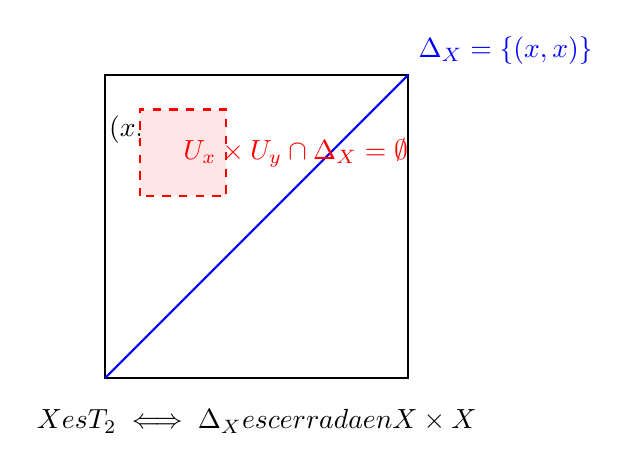
\begin{tikzpicture}[scale=1.1]
    \draw[thick] (0,0) rectangle (3.5,3.5);
    \draw[thick,blue] (0,0) -- (3.5,3.5) node[above right] {\(\Delta_X = \{(x,x)\}\)};
    \filldraw[black] (0.9,2.6) circle (1.8pt) node[above left] {\((x, y)\)};
    \draw[dashed,red,thick,fill=red!10] (0.4,2.1) rectangle (1.4,3.1);
    \node[red] at (2.2,2.6) {\(U_x \times U_y \cap \Delta_X = \emptyset\)};
    \node at (1.75,-0.5) {\(X \text{ es } T_2 \iff \Delta_X \text{ es cerrada en } X \times X\)};
\end{tikzpicture}
\end{center}

\begin{teo}[Teorema de Weierstrass de los valores extremos]
Sea \(K\) un espacio topológico compacto no vacío y \(f \colon K \to \mathbb{R}\) continua. Entonces \(f\) alcanza su máximo y su mínimo absolutos en \(K\).
\end{teo}

\begin{dem}
Por la Propiedad 1.3, la imagen \(f(K) \subseteq \mathbb{R}\) es compacta. Por el Teorema de Heine-Borel en \(\mathbb{R}\), \(f(K)\) es un subconjunto cerrado y acotado de \(\mathbb{R}\). Al ser acotado y no vacío, existen \(M \coloneqq \sup f(K)\) y \(m \coloneqq \inf f(K)\) en \(\mathbb{R}\). Por ser \(f(K)\) cerrado, se verifica que \(M \in f(K)\) y \(m \in f(K)\). Por tanto, existen puntos \(x_{\max}, x_{\min} \in K\) tales que:
\[
    f(x_{\max}) = M = \max_{x \in K} f(x), \qquad f(x_{\min}) = m = \min_{x \in K} f(x).
\]
\end{dem}
\end{comment} \cleardoublepage \chapter{Aplicaciones continuas} \justifying
Sean $(X, \mc T_X)$ e $(Y, \mc T_Y)$ dos espacios topol\'ogicos.
\begin{defi}
    Una aplicaci\'on de conjuntos $f: X\longrightarrow Y$ es \textbf{continua} (como espacios topol\'ogicos) si se verifica que $f^*(\mc T_Y) \subseteq \mc T_X$ siendo $f^* : \mc P(Y) \longrightarrow \mc P(X)$. 
\end{defi}
\begin{obs}
    Esta definci\'on es equivalente a decir que para $V \in \mc T_Y$ abierto, entonces $f^*(V) = f^{-1}(V) \in \mc T_X$. Es decir, que la antiimagen por $f$ de cualquier abierto de $Y$ es abierto en $X$. 
\end{obs}
\begin{prop}
    Se verifica que las siguientes condiciones son equivalentes:
    \begin{enumerate}
        \item $f$ es continua ($f^{-1}(V)$ es abierto en $X$, para todo $V\subset Y$  abierto). 
        \item $f^{-1}(C)$ es cerrado en $X$ para todo cerrado $C\subset Y$.
        \item Para todo $x\in X$, y todo entorno $W$ de $f(x)$ en $Y$, $f^{-1}(W)$ es entorno de $x$ en $X$. (No se puede hacer sobre $Y$ porque no se tienen puntos sobre los que hacer entorno en $X$).
        \item Si $\mc B$ es una base de la topolog\'ia por abiertos de $Y$, $f^{-1}(B) $ es abierto en $X$ para todo $B \in \mc B$. 
        \item Si $\mc B$ es base de cerrados de la topolog\'ia en $Y$, $f^{-1}(B)$ es cerrado en $X$ para todo $B\in \mc B$.
        \item Si $\{\mc B(y)\}_{y \in Y}$ es una base de entornos de la topolog\'ia de $Y$ entonces $f^{-1}(B)$ es entorno de $x$ para todo $B \in \mc B(f(x))$ y $\forall \, x \in X$.  
    \end{enumerate}
\end{prop}
\begin{dem}
    $1)\Rightarrow 2)$ $\forall \, Z \subset Y$ subconjunto, $f^{-1}(Y-Z) = X-f^{-1}(Z)$. 

    $1)\Rightarrow 3)$ Sea $W$ entorno de $f(x)\subset Y$. Por tanto, existe $V$ abierto en $Y$ tal que $f(x) \in V \subset W$, por lo que 
    $$x\in f^{-1}(f(x)) \subset f^{-1}(V) \subset f^{-1}(W)$$
    donde $f^{-1}(V)$ abierto de $X$ por la condici\'on 1) y entorno de $x$, como quer\'iamos ver.
    
    $3) \Rightarrow 1)$ Sea $V \subset Y$ abierto, veamos que $f^{-1}(V) \subset X$ es abierto. Veamos para ello que $\forall \, x\in f^{-1}(V), \, f^{-1}(V)$ es entorno de $x$. 

    $V$ es abierto de $Y$ y $f(x) \in V \Rightarrow V$ es entorno de $f(x)$, y $f^{-1}(V)$ es entorno del punto $x$. 
    
    $1) \Rightarrow 4)$

    $4) \Rightarrow 1)$ Sea $V \subset Y$ abierto $\Rightarrow V = \displaystyle \bigcup_{\overset{i\in I}{B_i \in \mc B} \, } B_i \Rightarrow f^{-1}(V) = \bigcup f^{-1}(B_i)$ siendo $f^{-1}(V) $ y $f^{-1}(B_i)$ abiertos. Si $\mc B$ es una base de la topolog\'ia por abiertos de $Y$, $f^{-1}(B)$ es abierto en $X$ para todo $B\in \mc B$. 
    
    $2) \iff 5)$ De la misma forma con intersecciones. 

    $3) \iff 6)$ \textcolor{red}{Terminar}
\end{dem}
\begin{defi}
    Una aplicaci\'on continua es \textbf{inyectiva} o \textbf{epiyectiva} si lo es como aplicaci\'on de conjuntos.

    Una aplicaci\'on continua es \textbf{isomorfismo de espacios topológicos} (\textbf{homeomorfismo}) si es biyectiva si lo es como aplicaci\'on de conjuntos y $f^{-1}: Y \longrightarrow X$ es continua.
\end{defi}
\begin{ejem}
    \begin{itemize} 
        \item Dado un espacio topológico $(X,\mc T_X)$
        $$\bt (X, \mc T_X) \rar{\text{Id}_X} & (X, \mc T_X) \\[-5mm] x \rarmaps & x \et$$
        es un homeomorfismo
        \item Sea $X$ un conjunto
        $$\bt (X, \mc T_{dis}) \rar{\text{Id}_X} & (X, \mc T_{triv}) \\[-5mm] x \rarmaps & x \et$$
        es continua y biyectiva, pero la inversa 
        $$\bt (X, \mc T_{triv}) \rar{\text{Id}_X^{-1}} & (X, \mc T_{dis}) \\[-5mm] x \rarmaps & x \et$$
        no es continua pues para la antiimagen de un abierto de la discreta no podemos asegurar que sea abierto de la trivial, pues no tiene m\'as abiertos que $X$ y $\emptyset$. Esto nos dice que los homeomorfismos nos dan equivalencias entre las topologías de espacios. 
    \end{itemize}
\end{ejem}
\begin{prop}
    Sean $(X, \mc T_X)$ e $(Y, \mc T_Y)$ espacios topol\'ogicos y $f: (X, \mc T_X) \longrightarrow(Y, \mc T_Y)$ una aplicaci\'on continua. Sea $\mc T_X'$ y $\mc T_Y'$ otras topolog\'ias en $X$ e $Y$ respectivamente tales que $\mc T_X \subseteq \mc T_X'$, $\mc T_Y' \subseteq \mc T_Y$, entonces
    $$\bt f : (X, \mc T_X') \rar & (Y, \mc T_Y') \et \text{ es continua}$$
\end{prop}
\begin{dem}
    Como para todo abierto de $Y$ queremos que su antiimagen sea abierto en $X$, si tenemos una topolog\'ia m\'as pequeña en $Y$ es m\'as f\'acil que sea continua, y si en $X$ tenemos una topolog\'ia m\'as grande, es m\'as f\'acil a\'un que sea abierto, luego continua. \textcolor{red}{Formalizar}. 
\end{dem}
\begin{obs}
    Las aplicaciones constantes son continuas. Sea $y_o \in Y$, 
    $$\bt f_{y_o}: X \rar & Y \\[-5mm] \, \, x \rarmaps & y_o \et$$
    Si $V\subset Y$ es abierto,
    $$f^{-1}(V) = \begin{cases}
        X & \text{ si } y_o \in V \\ \emptyset & \text{ si } y_o \nin V
    \end{cases}$$
\end{obs}

\begin{prop}
Sea $f: X \longrightarrow Y$ una aplicación.
\begin{enumerate}
    \item Sea $(X, \mc T_X)$ un espacio topológico. Se verifica que para todo espacio topológico $(Y, \mc T_Y)$ y toda aplicación de conjuntos $f: X \longrightarrow Y$, esta es continua $\iff \mc T_X = \mc T_{\text{disc}}$ (máxima topología que se puede poner).
    \item Sea $(Y, \mc T_Y)$ un espacio topológico. Se verifica que para todo espacio topológico $(X, \mc T_X)$ y toda aplicación de conjuntos $f: X \longrightarrow Y$, esta es continua $\iff \mc T_Y = \mc T_i$ (mínima topología que se pueda poner en un espacio/conjunto).
\end{enumerate}
\end{prop}

\begin{dem}\begin{enumerate}
    \item $\Leftarrow)$ Si $\mc T_X = \mc T_{\text{disc}} \implies f: (X, \mc T_{\text{disc}}) \longrightarrow (Y, \mc T_Y)$ es continua, pues para todo abierto $V \in \mc T_Y$ se cumple $f^{-1}(V) \subseteq \mathcal{P}(X) = \mc T_{\text{disc}}$.
        
    $\Rightarrow)$ Sea $(X, \mc T_{\text{disc}}) = (Y, \mc T_Y)$.
        
        Tomamos $f = \text{Id}_X: (X, \mc T_X) \longrightarrow (X, \mc T_{\text{disc}})$, que por hipótesis debe ser continua.
        \[
            \begin{array}{ccc}
            A & \reflectbox{$\mapsto$} & \text{Id}_X^{-1}(A) = A \\
            \text{ab.} & & \text{ab.}
            \end{array}
        \]
        Como es continua, dado $A \in \mc T_{\text{disc}}$, $\text{Id}_X^{-1}(A) = A$ es abierto también en $(X, \mc T_X)$, luego $\mc T_{\text{disc}} \subseteq \mc T_X$. Como $\mc T_{\text{disc}}$ es la topología más grande, $\mc T_X \subseteq \mc T_{\text{disc}} \implies \mc T_X = \mc T_{\text{disc}}$.
    \item $\Leftarrow)$ Si $\mc T_Y = \mc T_i = \{\emptyset, Y\}$, para cualquier abierto $V \in \mc T_Y$, su preimagen es $f^{-1}(\emptyset) = \emptyset \in \mc T_X$ o $f^{-1}(Y) = X \in \mc T_X$, por lo que $f$ siempre es continua.

        $\Rightarrow)$  Supongamos que la condición se cumple para todo espacio topológico $(X, \mc T_X)$ y toda aplicación $f$. Tomamos $(X, \mc T_X) = (Y, \mc T_i)$ con la topología indiscreta y la aplicación identidad $f = \text{Id}_Y: (Y, \mc T_i) \longrightarrow (Y, \mc T_Y)$. Por hipótesis, esta identidad debe ser continua. Dado cualquier abierto $V \in \mc T_Y$, la preimagen $\text{Id}_Y^{-1}(V) = V$ debe ser un abierto en $(Y, \mc T_i) = \{\emptyset, Y\}$. Por lo tanto, necesariamente $V = \emptyset$ o $V = Y$, concluyendo que $\mc T_Y = \mc T_i$.
\end{enumerate}
\end{dem}

\begin{ejem}
En $(\mathbb{R}, \mc T_u)$:
\[
    [0, 1] \simeq [a, b] \quad \text{con } a < b
\]
\[
    (0, 1) \simeq (a, b) \quad \text{homeomorfos}
\] Estiramos el intervalo $[0, 1]$ con una homotecia multiplicando por $(b - a)$:
$$ \bt 
    \left[0, 1\right] \rar{h_{(b-a)}} & \left[0, b - a\right] \\[-5mm] 
    z \rarmaps & (b - a)z &[-13mm]  \text{continua (lo sabemos)} \\[-5mm] 
    \frac{1}{b - a} w & \arrow[mapsto]{l} w &[-13mm]  \text{la inversa es otra homotecia (continua)}
    \et $$
Luego es un homeomorfismo porque ambas homotecias tienen inversa y su inversa (otra homotecia) es continua. Ahora hacemos una traslación:
$$ \bt
    \left[0, b-a\right] \rar{T_a} & \left[a, b\right] \\[-5mm] 
    w \rarmaps & w + a & \text{continua} \\[-5mm]
    z - a & \arrow[mapsto]{l} z & \text{continua}
    \et $$

Luego:
\[
    [0, 1] \xrightarrow[\sim]{h_{b-a}} [0, b-a] \xrightarrow[\sim]{T_a} [a, b]
\]
\end{ejem}
\begin{ejem}[$(\mathbb{R}, \mc T_u)$]
Estirar un intervalo abierto hasta (cubrir) $\mathbb{R}$ también es homeomorfismo:
\[
    (a, b) \simeq \mathbb{R}
\]

Tomamos la semicircunferencia centrada en $(0,2)$, $SC_{(0,2)}$.

Como una circunferencia centrada en ese punto sería $\mathcal{C}_{(0,2)} \equiv x^2 + (y-2)^2 = 1$, la ecuación de la semicircunferencia es:
\[
    SC_{(0,2)} \equiv x^2 + (y-2)^2 = 1 \quad \text{con } 1 \le y < 2 \quad \subseteq (\mathbb{R}^2, \mc T_u).
\]

Ahora queremos proyectar esa semicircunferencia al intervalo $(-1, 1)$. Consideramos la aplicación:
$$\bt
    SC_{(0,2)}  \rar{\sim} & (-1, 1) \simeq  (a, b) \\[-5mm]
    (x, y)  \rarmaps & x &[-13mm] \text{continua} \\[-5mm]
    \left(z, 2 - \sqrt{1 - z^2}\right) & \arrow[mapsto]{l} z &[-13mm] \text{continua} &[-13mm] & \text{(todas las operaciones son continuas)}
   \et $$

Por tanto, esta aplicación es un homeomorfismo. Al final, solo estamos ``aplastando una circunferencia''. Como $(-1, 1)$ es homeomorfo a cualquier intervalo $(a, b)$, ya que hemos visto que $(-1, 1) \simeq (a, b)$.

Ahora vemos que $SC_{(0,2)} \simeq \mathbb{R}$. Tomamos la aplicación que consiste en unir cualquier punto de la circunferencia con el $(0, 2)$ y cortar esa recta con el eje $\mathbb{R}$ ($y = 0$).

La recta que une cualquier punto $(x_0, y_0)$ de la circunferencia con $(0, 2)$ es:
\[r \equiv y - 2 = \frac{y_0 - 2}{x_0} x.\]
Queremos cortar con la recta $s \equiv y = 0$. Luego el punto resultante es $\left(x = \frac{-2x_0}{y_0 - 2}, 0\right)$.

Es decir, definimos la aplicación:
$$\bt SC_{(0,2)} = (a,b) \rar{\sim} & \mathbb{R} \\[-5mm] (x_0, y_0) \rarmaps & \frac{-2x_0}{y_0 - 2} &[-10mm] \text{continua} \\[-5mm] \left( \pm \frac{2}{\sqrt{4 + z_0^2}}, \frac{2z_0^2}{4 + z_0^2} + 2 \right) & \arrow[mapsto]{l} z_0 & \text{continua} \et$$
Por tanto, $(a, b) \simeq \mathbb{R}$ homeomorfo.
\end{ejem}
\begin{ejer}
Demostrar que $\mathcal{C}_{(0,0)} \setminus \{N\} \simeq \mathbb{R} \simeq SC_{(0,0)}$. Siendo $N$ el punto $(0, a)$ tal que $a$ es el máximo o el mínimo valor que toma el eje vertical en la esfera/circunferencia.

La ecuación de la circunferencia es $x^2 + y^2 = b$.
$$\bt \mathcal{C}_{(0,0)} \setminus \{N\} \rar{\sim} & \mathbb{R} \\[-5mm] (x_0, y_0) \rarmaps & \dots \et$$
\begin{center}
\begin{tikzpicture}[scale=1.6, >=stealth]
    % Radio de la circunferencia
    \def\R{1.3}
    
    % Coordenadas clave
    \coordinate (O) at (0,0);
    \coordinate (N) at (0,\R);
    \coordinate (S) at (0,-\R);
    
    % Circunferencia centrada en el origen
    \draw[thick] (O) circle (\R cm);
    
    % Ejes principales (cruzan completamente)
    \draw (-2.3, 0) -- (2.3, 0); % Eje horizontal (R)
    \draw (0, -1.7) -- (0, 1.7); % Eje vertical (N - S)
    
    % -------------------------------------------------------------
    % RECTA DERECHA: Pasa por N(0, R) y por un punto P_right de la circunferencia
    % Ángulo de P_right = 35° => P_right = (R*cos(35°), R*sin(35°))
    % Intersección exacta con el eje y = 0: x = R * cos(35°) / (1 - sin(35°))
    % -------------------------------------------------------------
    \coordinate (Pright) at ({ \R*cos(35) }, { \R*sin(35) });
    \coordinate (Xright) at ({ \R*cos(35)/(1 - sin(35)) }, 0);
    
    % Dibujamos la recta prolongada
    \draw ($(N)!-0.15!(Xright)$) -- ($(N)!1.1!(Xright)$);
    
    % -------------------------------------------------------------
    % RECTA IZQUIERDA: Pasa por N(0, R) y corta al eje horizontal en x_left < 0
    % Tomamos el corte en x = -0.8
    % Intersección con la circunferencia: ángulo = -118.07° aprox.
    % -------------------------------------------------------------
    \coordinate (Xleft) at (-0.8, 0);
    \coordinate (Pleft) at ({ -2*\R*\R*(-0.8) / ((-0.8)*(-0.8) + \R*\R) }, { \R*( (-0.8)*(-0.8) - \R*\R ) / ((-0.8)*(-0.8) + \R*\R) });
    
    % Dibujamos la recta prolongada
    \draw ($(N)!-0.15!(Xleft)$) -- ($(N)!1.55!(Xleft)$);
    
    % -------------------------------------------------------------
    % PUNTOS Y ETIQUETAS
    % -------------------------------------------------------------
    \filldraw (N) circle (1.2pt) node[above right] {$N$};
    \filldraw (S) circle (1.2pt) node[below right] {$S$};
    \filldraw (O) circle (1pt) node[below right] {$(0,0)$};
    
    % Puntos sobre la recta derecha
    \filldraw (Pright) circle (1.2pt);
    \filldraw (Xright) circle (1.2pt);
    
    % Puntos sobre la recta izquierda
    \filldraw (Xleft) circle (1.2pt);
    \filldraw (Pleft) circle (1.2pt);
\end{tikzpicture}
\end{center}
\end{ejer}

\begin{ejer}
Sea $X$ un espacio topológico. $A \subseteq X$ es subespacio topológico $\iff (A, \mc T_X\vert{}_A)$.
$$\bt (A, \mc T_X\vert{}_A) \rar[hook]{i_A} & (X, \mc T_X) \\[-5mm] a \rarmaps & a & [-12mm] \text{continua} \et$$
$i_A$ es continua porque $i_A^*(\mc T_X) = \mc T_X\vert{}_A$.
\end{ejer}
\noindent \textbf{Nota}.  Para definir aplicaciones, primero mira una aplicación entre conjuntos y luego comprueba si es continua.

\begin{propis}[de las aplicaciones continuas] \, 
\begin{enumerate}
    \item Si $X, Y, Z$ son espacios topol\'ogicos y $f: X \longrightarrow Y$, $g:Y \longrightarrow Z$ son aplicaciones continuas, entonces $g \circ f : X \longrightarrow Z$ es continua.
    \item Si $f: X \longrightarrow Y$ es continua y $A \subset X$ es subespacio topol\'ogico, entonces 
    $$\bt f\vert{}_A : A \rar & Y  \\[-5mm] a \rarmaps & f\vert{}_A(x) \coloneqq f(x) \et$$
    es continua.
    \item Si $f: X \longrightarrow Y$ es continua y $B\subset Y$ subespacio topol\'ogico con $\Im \, f\subset B$, entonces 
    $$\bt f^B: X \rar & B \\[-5mm] x \rarmaps & f(x) \et$$
    es continua.
    \item Sea $f: X\longrightarrow Z$ aplicaci\'on continua con $Z \subset Y$ subespacio topol\'ogico, entonces 
    $$\bt f^Y: X \rar & Y \\[-5mm] x \rarmaps & f(x) \et$$
    es continua.
    \item Si $\{U_i\}_{i \in I}$ es un recubrimiento por abiertos de $X$ ($X = \bigcup U_i$), y sea $f: X \longrightarrow Y$ una aplicaci\'on de conjuntos tal que $f\vert{}_{U_i} : U_i \longrightarrow Y$ es continua para todo $i\in I$, entonces $f$ es continua (equivalentemente diremos que la continuidad de una aplicaci\'on es un concepto local). 
\end{enumerate}
\end{propis}
\begin{dem}\, 
    \begin{enumerate}
        \item Sea $W\subset Z$ un abierto, veamos que $(g\circ f)^{-1}(W) \subset X$ es abierto. 
        
        Como $(g\circ f)^{-1}(W) = f^{-1}(g^{-1}(W))$ y $g$ es continua, $g^{-1}(W) \subset Y$ es abierto, de forma que como $f$ tambi\'en es continua y $V = g^{-1}(W) \subset Y$ es abierto, $f^{-1}(V) = f^{-1}(g^{-1}(W))$ es abierto en $X$, como quer\'iamos demostrar. 
        
        \noindent \textbf{Observaci\'on:} $(g\circ f)^{-1}(W) \neq (f^{-1} \circ g^{-1})(W)$ pues $f^{-1}$ y $g^{-1}$ NO existen como aplicaci\'on. 

        \item $\bt A \rar[hook]{i_A} & X \rar{f} & Y \et$ de forma que $f\vert{}_A = f\circ i_A$ composici\'on de aplicaciones continuas, por 1., continua. 
        
        \item Sea $W \subset B$ un abierto de $B$, por lo que por ser la topolog\'ia inducida en $Y$, existe $U\subset Y$ abierto de $Y$ tal que $V \cap B = W$. Entonces $f^{-1}(V) \subset X$ es abierto por ser $f$ continua, pero $f^{-1}(V)  = f^{-1}(V \cap \Im f) = f^{-1}(V \cap B) = f^{-1}(W)=(f^B)^{-1}(W)$ poque $\Im f\subset B$.  
        \item Similar a 3.
        \item Sea $V\subset Y$ abierto y veamos que $f^{-1}(V)$ es abierto. $f^{-1}(V) \subset X$ luego
        $$f^{-1}(V) = f^{-1}(V) \cap X = f^{-1}(V) \cap \left( \bigcup_{i \in I} U_i \right) = \bigcup_{i\in I} \left(f^{-1}(V) \cap U_i \right) = \bigcup_{i \in I} f\vert{}_{U_i}^{-1}(V)$$
        por ser $f\vert{}_{U_i} ^{-1}(V)$ abierto en $U_i$ (que es abierto), son abiertos en $X$ $\forall \, i$, la uni\'on arbitraria de abiertos es abierto y por tanto $f^{-1}(V)$ es abierto como quer\'iamos demostrar. 
    \end{enumerate}
\end{dem}
\begin{defi}
    Una apliaci\'on de conjuntos $f : X\longrightarrow Y$ entre espacios topol\'ogicos, entonces se dice que $f$ es \textbf{continua en un punto $x\in X$} si para todo entorno $V$ de $f(x)$, $f^{-1}(V)$ es entorno de $x$ en $X$. 

    Se verifica que $f$ es continua si y solo si $f$ es continua en todos los puntos de $X$. 
\end{defi}
Sea $f: X\longrightarrow Y$ aplicaci\'on continua
\begin{propis}
[negativas] Si $V \subset Y$ es abierto $\Rightarrow$ $f^{-1}(V)$ es abierto en $X$. Su rec\'iproco es falso, si $V\subset Y$ es un subconjunto tal que $f^{-1}(V) \subset X$ es abierto $\not\Rightarrow V \subset Y$ sea abierto. Por $\text{Id}: (X, \mc T_{dis}) \longrightarrow (X, \mc T_{triv})$ que es continua se demuestra. 

Sea $U\subset X$ abierto $\not\Rightarrow f(U)$ es abierto en $Y$. 
$$\bt \bb R \rar{f} & \bb R \\[-5mm] x \rarmaps & x^2 \\[-5mm] (-2,2) \rarmaps & \left[0,4\right) \et$$
de forma que la imagen de un abierto $(-2,2)$ no es abierto $[0,4)$
\end{propis}
\begin{defi}
    Una aplicaci\'on de conjuntos $f : X \longrightarrow Y$ entre espacios topol\'ogicos es \textbf{abierta} si para todo abierto $U$ de $X$, $f(U)$ es abierto en $Y$ (no suponer que $f$ sea continua).
\end{defi}
\begin{ejem}
    $\text{Id}: (X, \mc T_{triv}) \longrightarrow (X, \mc T_{dis})$ es abierta pero no continua.
\end{ejem}
\begin{defi}
Una aplicaci\'on de conjuntos $f : X \longrightarrow Y$ entre espacios topol\'ogicos es \textbf{cerrada} si para todo cerrado $C$ de $X$, $f(C)$ es cerrado en $Y$ (no suponer que $f$ sea continua).
\end{defi}
\begin{ejer}
    Sea $X$ un espacio topol\'ogico y $A\subset X$ un subespacio topol\'ogico, $i_A: A \hookrightarrow X$ es continua. Se verifica que 
    \begin{itemize}
        \item $i_A$ es abierta $\iff \, A \subset X$ es abierto
        \item $i_A$ es cerrada $\iff \, A \subset X$ es cerrada. 
    \end{itemize}    
\end{ejer}

\begin{ejer}
    Aplicaci\'on abierta $\not\Rightarrow$ cerrada. 
\end{ejer}
\begin{sol}
    No, porque el complementario no funciona bien con la imagen. Sea $C = X-U, \, f(C) = f(X-U) \neq Y - f(U)$ (con la antiimagen s\'i).
\end{sol}

Sea $f: X \longrightarrow Y$ una aplicaci\'on continua
\begin{defi}
    Decimos que $f$ es una \textbf{inmersión topológica} si $f$ establece un homeomorfismo 
    $$\bt f: X \rar{\sim} & (\Im f, \mc T_Y \vert{} _{\Im f}) \et \Rightarrow \bt f: X \arrow[swap]{rd}{\sim} \rar[hook] & Y \\[-5mm] & \Im f \arrow[phantom]{u}{\cup}  \et \text{ es inyectiva.}$$
    (No es que sean homeomorfos, es a trav\'es de $f$) ($X$ se identifica con el subespacio topol\'ogico imagen)
\end{defi}
\begin{ejem}
    Si $X$ es espacio topol\'ogico, $A \subset X$, 
    $$\bt (A, \mc T_X\vert{}_A) \arrow[swap]{rd}{\Id_A} \rar[hook]{i_A} & (X, \mc T_X) \\  & (\Im i_A = A, \mc T_X \vert{} _A) \et$$
\end{ejem}
\begin{defi}
    Una \textbf{función de $X$} es una aplicaci\'on $f: X\longrightarrow \bb Q$ \'o $f: X\longrightarrow \bb C \simeq \bb R^2$
\end{defi}

\section{Topolog\'ia inicial}
\begin{custom}
[Motivaci\'on] Si $f: X \longrightarrow Y$ es una aplicaci\'on continua, 
$$\bt f^* : \mc P(Y) \rar & \mc P(X) \\[-5mm] \mc T_Y \rarmaps & f^*(\mc T_Y) \subset \mc T_X \et$$
$f^*(\mc T_Y)$ es la topolog\'ia menos fina (m\'as pequeña) en $X$ que hace a $f$ continua (si tenemos otra topolog\'ia que no la contenga, $f$ no es continua). 
\end{custom}
Sea $(Y, \mc T_Y)$ un espacio topol\'ogico, $X$ un conjunto y $f:X \longrightarrow Y$ una aplicaci\'on de conjuntos
\begin{defi}
    Se define la \textbf{topología inicial de la aplicación $f$} como la topolog\'ia en $X$ dada por 
    $$\bt f^* : \mc P(Y) \rar & \mc P(X) \\[-5mm] \mc T_Y \rarmaps & f^*(\mc T_Y)  \et$$
    Es la topolog\'ia menos fina que en $X$ que hace a la aplicaci\'on de conjuntos $f: X\longrightarrow Y$ continua
    $$f^*(\mc T_Y) \equiv \mc T_f = \{U \subset X : \text{ existe } V \text{ abierto en } Y \text{ tal que } f^*(V) = f^{-1}(V) = U\}$$
\end{defi}\begin{ejem}
    Sea $(X, \mc T_X)$ espacio topol\'ogico y $A \subset X$ un subconjunto, para $i_A: A \hookrightarrow X$ se tiene que 
    $$\mc T_{i_A} = i_A^*(\mc T_X) = \mc T_X\vert{}_A$$
\end{ejem}

Sean $\{(X_i, \mc T_{Y_i})\}_{i \in I}$ espacios topol\'ogicos, $X$ un conjunto y $\{f_i : X \longrightarrow Y_i\}_{i \in I}$ aplicaciones de conjuntos
\begin{defi}
    La \textbf{topología inicial en $X$ de las aplicaciones $\{f_i\}_{i \in I}$}, denotada por $\mc T_{\{f_i\}_{i \in I}}$, es la topolog\'ia menos fina en $X$ que hace que todas las aplicaciones de conjuntos $f_i: X \longrightarrow Y_i$ sea continuas $\forall \, i \in I$
    $$\bt f^*_i : \mc P(Y_i) \rar & \mc P(X) \\[-5mm] \mc T_{Y_i} \rarmaps & f^*(\mc T_{Y_i}) = \mc T_{f_i} \et \Rightarrow   \, \, \mc T_{f_i} \text{ tiene que contener a todas las topolog\'ias } \{f^*_i(\mc T_{Y_i})\}$$
    (ver el subconjunto m\'as pequeño de $\mc P(X)$ que las contiene).
\end{defi} 
\begin{obs}
    $\displaystyle \bigcup_{i \in I} f_i^*(\mc T_{Y_i}) \subset \mc P(X)$ no tiene por qu\'e ser topolog\'ia, pues la uni\'on arbitraria no lo asegura. La intersecci\'on s\'i.

    Buscamos la menor topolog\'ia que lo contenga. No es topolog\'ia ni base, pero es subbase de una topolog\'ia. 

    En efecto, sea $x\in X, \, i \in I, Y_i \in \mc T_{Y_i}, \, X\in f_i^*(Y_i) \in \bigcup f_i^*(\mc T_{Y_i})$, $f_i^*(Y_i) = f_i^{-1}(Y_i)=X$.

    La menor topolog\'ia que la contiene es la generada por esa sub-base 
    $$S\mc B_{\{f_i\}} = \bigcup_{i \in I} f_i^*(\mc T_{Y_i}) = \{ U \subset X : \text{ para alg\'un } i \in I, \, U \in f_i^*(\mc T_{Y_i}) \equiv \text{ existe } V_i \in \mc T_{Y_i} \text{ tal que } f_i^{-1}(V_i) = U\}$$

    Consideremos $\mc B_{\{f_i\}}$ la base generada por $S\mc B_{\{f_i\}}$
    $$\mc B_{\{f_i\}} = \{f_{i_1}^{-1}(V_{i_1}) \cap \cdots \cap f_{i_r}^{-1}(V_{i_r}) \text{ con } i_1, \ldots, i_r \in I, \, V_{i_j} \subset Y_{i_j}\text{ abierto para cada } j \in \{i_1, \ldots, i_r\}\}$$

    La topolog\'ia 
    $$\mc T_{\{F_i\}} \equiv \left\{ \text{topolog\'ia generada por } \mc B^{\{f_i\}} \right\} = \left\{\bigcup_{\underset{i_1, \ldots, i_r \in I}{r \in \bb N}} f^{-1}_{i_1}(V_{i_1}) \cap \cdots \cap f^{-1}_{i_r}(V_{i_r})\right\}$$
    es la uni\'on arbitraria de intersecciones finitas de antiim\'agenes de abiertos, que ahora s\'i podemos asegurar que sea una toolog\'ia. 
\end{obs}

\medskip

Sean $\{f_i : X\longrightarrow (Y_i, \mc T_{Y_i})\}_{i \in I}$ aplicaciones de conjuntos.
\begin{propi}
    [Universal de la Topolog\'ia inicial] La topolog\'ia inicial de las aplicaciones $\{f_i\}_{i \in I}, \, \mc T_{\{f_i\}}$ en $X$ es la \'unica topolog\'ia de $X$ que verifica que para todo espacio topol\'ogico $(Z, \mc T_Z)$ y toda aplicaci\'on $g: Z \longrightarrow X$
    $$g \text{ es continua con  } (X, \mc T_{\{f_i\}}) \iff f_i \circ g: Z \longrightarrow Y_i \text{ es continua } \forall i \in I$$
\end{propi}
\begin{dem}
$\Rightarrow)$ $g$ es continua y $f_i$ tambi\'en para todo $i\in I$ por la topolog\'ia inicial, por lo que  
$$\bt Z \rar{g} \arrow[bend right=10mm,swap]{rr}{f_i \circ g} & X \rar{f_i} & Y_i \et$$
como la composici\'on de aplicaciones continuas es continua, aseguramos que $g\circ f_i$ es continua.

$\Leftarrow)$ Supongamos que $f_i \circ g$ es continua $\forall i \in I$.

Para comprobar que $g$ es continua, basta comrpobar que $g^{-1}(f_i^{-1}(U_i)) \subset Z$ es abierto para cada $i \in I$ y para cada $V_i \subset Y_i$
$$Z \subset g^{-1}(f_i^{-1}(V_i)) = (\underbrace{f_i \circ g}_{\text{continua}})^{-1}(V_i) $$
asegurando as\'i que es un abierto en $Z$.
\end{dem}

\medskip

\begin{prop}
Sea $X$ un conjunto, $\{ (Y_i, \mc T_{Y_i}) \}_{i \in I}$ una familia de espacios topológicos y $\{f_i \colon X \longrightarrow Y_i\}_{i \in I}$ una familia de aplicaciones. Si $\mc T_X$ es una topología en $X$ que satisface la propiedad universal de la topología inicial, entonces:
\[
    \mc T_X = \mc T_{\{f_i\}}
\]
\end{prop}

\begin{dem}
Las aplicaciones $f_i \colon (X, \mc T_X) \longrightarrow (Y_i, \mc T_{Y_i})$ son continuas para todo $i \in I$. En efecto, al considerar la aplicación identidad $\operatorname{Id}_X \colon (X, \mc T_X) \longrightarrow (X, \mc T_X)$, se tiene 
\[
\bt (X, \mc T_X) \rar{\operatorname{Id}_X} \arrow[bend right=10mm]{rr}{f_i} & (X, \mc T_X) \rar{f_i} & Y_i \et
\]
Dado que $\operatorname{Id}_X$ es continua, la composición $f_i = f_i \circ \operatorname{Id}_X$ es continua. Por la definición de topología inicial (al ser la menos fina que hace continuas a las $f_i$), se deduce que
\[
    \mc T_{\{f_i\}} \subseteq \mc T_X.
\]

Recíprocamente, por la propiedad universal de la topología inicial $\mc T_{\{f_i\}}$, la aplicación identidad $\operatorname{Id}_X \colon (X, \mc T_X) \longrightarrow (X, \mc T_{\{f_i\}})$ es continua si y solo si lo es la composición
\[
\bt (X, \mc T_X) \rar{\operatorname{Id}_X} \arrow[bend right=10mm]{rr}{f_i} & (X, \mc T_X) \rar{f_i} & Y_i \et
\]
Como las aplicaciones $f_i$ son continuas por hipótesis sobre $\mc T_X$, se deduce que $\operatorname{Id}_X \colon (X, \mc T_X) \longrightarrow (X, \mc T_{\{f_i\}})$ es continua. Por tanto
\[
    \mc T_X \subseteq \mc T_{\{f_i\}}.
\]

Concluimos que $\mc T_X = \mc T_{\{f_i\}}$.
\end{dem}

\section{Producto directo de espacios topol\'ogicos}

Sean $\{(X_i,\mc T_i)\}_{i\in I}$  una familia de espacios topol\'ogicos. Sea $\{X_i\}_{i \in I}$ una familia de conjuntos, se tiene el conjunto
$$\prod_{i\in I} X_i = \left\{ (x_i)_{i\in I} : x_i \in X_i \right\}$$
Para cada $j\in I$, se tiene la aplicaci\'on de conjuntos
$$\bt \pi_j : \displaystyle \prod_{i \in I} X_i \rar & X_j \\[-5mm] (x_i)_{i\in I} \rarmaps & x_j \et$$

Sea $\mc T_{\{\pi_j\}_{j \in I}}$ la topolog\'ia inicial en $\prod_{i \in I} X_i$ de las proyecciones can\'onicas $\{\pi_j: \prod_{i \in I} X_i \longrightarrow X_j\}_{j \in I}$, la llamamos topolog\'ia del producto directo, $\mc T_{\pi}$ en $\prod_{i \in I} X_i$.

El espacio topol\'ogico producto directo de espacio topol\'ogicos $\{(X_i, \mc T_i)\}_{i\in I}$ es por definici\'on $\left(\prod_{i \in I} X_i, \mc T_{\pi} \right)$

\section{Base de la topología producto directo ($\mc T_{\pi}$)}

Dada una familia de espacios topológicos $\{(X_i, \mc T_{X_i})\}_{i \in I}$, un elemento de la base de la topología inicial por las proyecciones canónicas $\pi_i \colon \prod_{i \in I} X_i \longrightarrow X_i$ viene dado por la intersección finita de antiimágenes de abiertos:
\[
    \pi_{i_1}^{-1}(U_{i_1}) \cap \cdots \cap \pi_{i_r}^{-1}(U_{i_r}) = V \quad (\text{elemento de la base de la topología producto directo}).
\]

\paragraph{Caso de dos factores ($I = \{1, 2\}$):}
Consideremos $I = \{1, 2\}$. Se tiene que
\[
    \pi_1^{-1}(U_1) \cap \pi_2^{-1}(U_2) = \textcolor{green}{U_1 \times U_2}.
\] por la siguiente figura podemos observarlo

\begin{center}
\begin{tikzpicture}[scale=1]
    % Ejes
    \draw[thick, ->] (-0.5,0) -- (4.5,0) node[below right] {$X_1$};
    \draw[thick, ->] (0,-0.5) -- (0,3.5) node[above left] {$X_2$};

    % Intervalo U1 en X1
    \draw[very thick, blue] (1.2,0) -- (2.8,0);
    \node[blue, below] at (2, -0.1) {$U_1$};
    \draw[blue] (1.2,0.1) -- (1.2,-0.1);
    \draw[blue] (2.8,0.1) -- (2.8,-0.1);

    % Intervalo U2 en X2
    \draw[very thick, red] (0,1.5) -- (0,2.5);
    \node[red, left] at (-0.1, 2) {$U_2$};
    \draw[red] (0.1,1.5) -- (-0.1,1.5);
    \draw[red] (0.1,2.5) -- (-0.1,2.5);

    % Lineas discontinuas de proyeccion
    \draw[dashed, blue] (1.2,-1) -- (1.2,4);
    \draw[dashed, blue] (2.8,-1) -- (2.8,4);
    \draw[dashed, red] (-1,1.5) -- (4,1.5);
    \draw[dashed, red] (-1,2.5) -- (4,2.5);

    % Rectangulo producto U1 x U2 rayado
    \fill[pattern=north east lines, pattern color=green!70] (1.2,1.5) rectangle (2.8,2.5);
    \draw[thick] (1.2,1.5) rectangle (2.8,2.5);

    % Flechas de proyeccion y etiquetas
    %\node at (2, 2.9) {$X_1 \times X_2$};
    \draw[<-, thick, blue] (3.1,0.5) -- (3.1, 1.8) node[above] {$\pi_1$};
    \draw[<-, thick, red] (0.5,2.8) -- (2,2.8) node[right] {$\pi_2$};
    \node[blue] at (2,3.8)  {$\pi_1^{-1}(U_1)$};
    \node[red] at (4.7, 2) {$\pi_2^{-1}(U_2)$};
\end{tikzpicture}
\end{center}
de forma que 
\[
    \pi_1^{-1}(U_1) = U_1 \times X_2 \subseteq X_1 \times X_2, \qquad \pi_2^{-1}(U_2) = X_1 \times U_2 \subseteq X_1 \times X_2.
\]

\noindent \underline{Caso finito}. ($I = \{1, \ldots, n\}$):
Si $U_1 \subseteq X_1, \ldots, U_n \subseteq X_n$, la topología coincide con la topología de las cajas
\[
    \mc T_\pi = \mc T_{\text{cajas}} = \left\langle \{U_1 \times \cdots \times U_n \mid U_i \subseteq X_i \text{ abiertos}\} \right\rangle.
\]

\noindent \underline{Caso arbitrario}. Para un índice $i_1 \in I$ cualquiera
\[
    \pi_{i_1}^{-1}(U_{i_1}) = U_{i_1} \times \prod_{j \neq i_1} X_j = \left\{ (x_i)_{i \in I} \in \prod_{i \in I} X_i \;\middle|\; x_{i_1} \in U_{i_1} \right\}.
\]
Para un número finito de índices $\{i_1, \ldots, i_r\} \subseteq I$
\[
    \pi_{i_1}^{-1}(U_{i_1}) \cap \cdots \cap \pi_{i_r}^{-1}(U_{i_r}) = U_{i_1} \times \cdots \times U_{i_r} \times \prod_{j \notin \{i_1, \ldots, i_r\}} X_j.
\]
En cambio, la \textbf{topología de las cajas} sobre un producto arbitrario se define como:
\[
    \mc T_{\text{cajas}} = \left\langle \left\{ \prod_{i \in I} U_i \;\middle|\; U_i \subseteq X_i \text{ abiertos} \right\} \right\rangle.
\]

En general, para productos infinitos se verifica que $\mc T_\pi \subsetneq \mc T_{\text{cajas}}$.
\begin{custom}
    [Contraejemplo] $\prod_{n \in \bb N} \bb R = \bb R^{\bb N}$. Sus elementos son $(x_n)_{n \in \bb N}: x_n \in \bb R$, es decir, una sucesi\'on, por lo que $\bb R^{\bb N}$ es el espacio de sucesiones de n\'umeros reales. De esta forma, se tiene que $(\bb R^{\bb N}, \mc T_{\pi})$ y $(\bb R^{\bb N}, \mc T_{cajas})$, se tiene la aplicaci\'on de conjuntos,
    $$\bt \bb R \rar{c} & \bb R^{\bb N} \\[-5mm] \lambda \rarmaps & (\lambda)_{n\in\bb N}\et$$
     de forma que $c$ es continua en $(\bb R, \mc T_d)\longrightarrow (\bb R^{\bb N}, \mc T_{\pi})$ pero no en $(\bb R, \mc T_d)\longrightarrow (\bb R^{\bb N}, \mc T_{cajas})$.

     En efecto, por la propiedad universal, 
     $$\bt \bb R \rar{c} \arrow[bend left=10mm]{rr}{\text{Id}_X} & \bb R^{\bb N} \rar{\pi_n} & \bb R \\[-5mm] 
     \lambda \rarmaps & (\lambda)_{n \in \bb N} \rarmaps & \lambda
     \et$$ de forma que como $\pi_n$ es continua, $\text{Id}_X$ es continua, entonces $c$ es continua.

     Por otro lado, sea 
     $$\bb R^{\bb N} \supset U := (-1,1) \times (-\nicefrac{1}{2}, \nicefrac{1}{2}) \times \cdots \times (-\nicefrac{1}{n}, \nicefrac{1}{n}) \times \cdots $$
     es un abierto b\'asico en $\mc T_{cajas}$ por ser producto de abiertos, y al hacerle antiimagen por $c$, $\lambda \in (-\nicefrac{1}{n}, \nicefrac{1}{n})\forall n\in \bb N$, por lo que tiene que pertenecer a su intersecci\'on,  
     $$c^{-1} (U) = \bigcap_{n \in \bb N} (-\nicefrac{1}{n}, \nicefrac{1}{n}) = \{0\} \in \bb R$$
     que no es abierto, por lo que $c$ no es continua.
\end{custom}
\begin{ejer}
    Sean $X_i$ espacios topol\'ogicos y $f:X\longrightarrow Y$ aplicaci\'on continua e inyectiva. $f$ es inmersi\'on topol\'ogica si y solo si $\mc T_X = \mc T_f =$ topolog\'ia inicial de $f$. 
    
    (Falta comprobar que $f^{-1}$ sea continua sobre $\Im f$. Por ser $f$ continua, $\mc T_f \subset \mc T_X$, hay que comprobar la inclusi\'on contraria). 
\end{ejer}
\begin{ejer}
    Sea $X$ espacio topol\'ogico y $f,g$ funciones continuas en $X$. Definimos
    $$\bt X \rar{f+g} & \bb R \\[-5mm] x \rarmaps & (f+g)(x) = f(x) + g(x) \et$$
    y si $f,g$ son continuas, entonces $f+g$ es continua. Podemos ver que 
    $$\bt X \rar{(f,g)} & \bb R \times \bb R \rar{s} & \bb R \\[-5mm]
    x \rarmaps & (f(x),g(x)) \rarmaps & f(x)+g(x)
    \et$$
    de forma que $(f,g)$ es continua si y solo si las composiciones con $\pi_i$ lo son
    $$\bt & & \bb R \\[-5mm] X \arrow[bend left=8mm,swap]{rru}{g}  \arrow[bend right=8mm]{rrd}{f} \rar{(f,g)} & \bb R\times \bb R \arrow[swap]{ru}{\pi_1}\arrow{rd}{\pi_2} \\[-5mm] & & \bb R \et$$
    y como $f$ y $g$ son continuas y $\pi_i$ tambi\'en, $(f,g)$ tambi\'en, y la suma por tanto tambi\'en. De la misma forma, $f(x) \cdot g(x)$. 
\end{ejer}
\section{Topolog\'ia final}
\begin{custom}
    [Motivaci\'on] Sea $f: X \longrightarrow Y$ continua, tenemos $f^*: \mc P(Y) \longrightarrow \mc P(X)$ cumple que $f^*(\mc T_Y) \subset \mc T_X$. Pero es lo mismo que $\mc T_Y \subset (f^*)^{-1}(\mc T_X)$, esto es $(f^*)^{-1}(\mc T_X)$ es la topolog\'ia en $Y$ m\'as fina (m\'as grande, con m\'as abiertos) que hace a $f$ continua.
\end{custom}
Sea $(X, \mc T_X)$ espacio topol\'ogico, $Y$ un conjunto y $f: X \longrightarrow Y$ una aplicaci\'on de conjuntos. 
\begin{defi}
    La \textbf{topolog\'ia final} de $f$ es la topolog\'ia en $Y$ m\'as fina que hace a $f$ continua, y es $(f^*)^{-1}(\mc T_X) =: \mc T^f=\mc T_{f^*}$
    $$\mc T^f = \left\{ V \subset Y : f^*(V) \in \mc T_X  \right\} =  \left\{ V \subset Y : f^{-1}(V) \text{ es abierto en } X  \right\}$$
    (si $f$ es biyectiva es $\mc T_X$)
\end{defi}
\begin{ejer}
    Comprobar que $(f^*)^{-1}(\mc T_X)$ es topolog\'ia si $\mc T_X$ lo es.
\end{ejer}

Sean $\{(X_i,\mc T_i)\}_{i \in I}$ espacios topol\'ogicos, $Y$ un conjunto, $\{f_i: X_i \longrightarrow Y\}_{i \in I}$
\begin{defi}
    La \textbf{topolog\'ia final} de las aplicaciones $\{f_i : X_i \longrightarrow Y\}_{i \in I}$ en $Y$ es la topolog\'ia m\'as fina en $Y$ que hace a todas las aplicaciones $\{f_i\}_{i \in I}$ continuas. (Cualquier topolog\'ia en $Y$ que haga a las $f_i$ continuas est\'a contenida en $\mc T^{\{f_i\}}$). 

    Para que $f_i: X_i \longrightarrow (Y, \mc T_i)$ sea continua $Y$ tiene que tener $\mc T^{f_i}$. Es decir, $\mc T_i \subset \mc T^{f_i}$. Entonces, para que todas sean continuas cada $\mc T^{f_i}$ tiene que estar contenidas, es decir, es
    $$\mc T^{\{f_i\}} = \bigcap_{i \in I} \mc T^{f_i} = \left\{ V \subset Y : f_i^{-1}(V) \subset X_i \text{ es abierto}, \forall \, i \in I \right\}$$
\end{defi}
\begin{ejer}
    Probar que $\bigcap_{i \in I} \mc T_i$ es topolog\'ia si las $\mc T_i$ lo son.
\end{ejer}
\begin{propi}
[Universal de la topolog\'ia final] Sean $\{(X_i,\mc T_i)\}_{i \in I}$ espacios topol\'ogicos, $Y$ un conjunto y $\{f_i : X_i \longrightarrow Y\}_{i \in I}$ aplicaciones. La topolog\'ia final $\mc T^{\{f_i\}}$ de las aplicaciones $\{f_i\}_{i \in I}$ es la \'unica topolog\'ia en $Y$ que verifica la siguiente propiedad:

Para todo espacio topol\'ogico $(Z, \mc T_Z)$ y para toda aplicaci\'on $g: Y \longrightarrow Z$ (de conjuntos),
$$g \text{ es continua } \iff  g\circ f_i \text{ son continuas } \forall \, i \in I, \bt X_i \arrow[bend right=10mm]{rr}{g\circ f_i} \rar{f_i} & Y \rar{g} & Z \et$$
\end{propi}
\begin{dem}
    $\Rightarrow)$ $Y \xrightarrow{g} Z$ continua, $X_i \xrightarrow{f_i} (Y, \mc T^{\{f_i\}})$ continuas $\forall \, i\in I$, 
    $$\bt X_i \rar{f_i} \arrow[bend right=10mm]{rr}{g\circ f_i}  & Y \rar{g} & Z \et \text{ es continua por ser composici\'on de continuas. }$$
    $\Leftarrow)$ Sea $W \subset Z$ abierto, veamos que $g^{-1}(W)$ es abierto en $ (Y, \mc T^{\{f_i\}})$.
    
    Por la definici\'on de la topolog\'ia final, $g^{-1}(W)$ es abierto en $ (Y, \mc T^{\{f_i\}}) \iff f_i^{-1}(g^{-1}(W)) \subset X_i$ es abierto $\forall \, i \in I$, pero 
    $$f_i^{-1}(g^{-1}(W)) = (g\circ f_i)^{-1}(W)$$
    y $g\circ f_i$ es continua por hip\'otesis $\forall \, i \in I$, por lo que $g^{-1}(W)$ es un abierto. 
\end{dem}
\section{Topolog\'ia  uni\'on disjunta}
Sean $\{X_i\}_{i\in I}$ conjuntos, se define la unión disjunta de conjuntos
$$\coprod_{i \in I} X_i= \{(i, x_i) \, / \, x_i \in X_i, \, i \in I\}$$
que intuitivamente es ``dar un elemento de cada uno de los conjuntos''.
\begin{ejem}
    $\bb R \sqcup \bb R \ni (1,0) = O_1$ es el 0 de la primera copia de $\bb R$ y $(2,0)=O_2$ es el 0 de la segunda, de forma que todos los elementos est\'an repetidos, y gr\'aficamente son dos rectas que no tienen elementos comunes. 
\end{ejem}
\begin{ejem}
    Sean $A, B\subset X$ dos subconjuntos $A\cup B \subset X$ y $A\sqcup B$ son iguales si $A\cap B = \emptyset$. En caso contrario, si $A\cap B \neq \emptyset$,
    $$\bt A\sqcup B \rar & A\cup B \\[-5mm] (1,a) \rarmaps & a \\[-5mm] (2,b) \rarmaps & b \et$$
    es epiyectiva. Si $c\in A\cap B$, 
    $$\bt (1,c) \rarmaps & c \\[-5mm] (2,c) \arrow[mapsto]{ru} & \et$$
\end{ejem}
\begin{ejem}
    Sea $E$ espacio vectorial y $E_1, E_2 \subset E$ dos subespacios,
    $$\bt 0 \rar & E_1 \cap E_2 \rar & E_1 \oplus E_2 \rar & E_1+E_2 \rar & 0 \\[-5mm]
    & & (e_1,e_2) \rarmaps & e_1 + e_2 \rarmaps & 0 \\[-5mm] & e \rarmaps & (e,e)
    \et$$
    Aqu\'i la uni\'on disjunta es la suma directa de espacio vectoriales $\displaystyle \bigoplus_{i \in I} E_i \subset \prod_{i \in I} E_i$ est\'a contenido en el producto directo. 
\end{ejem}
Para cada $j \in I$, se tiene la inmersi\'on
$$\bt \varphi_j : X_j \rar[hook] & \coprod X_i \\[-5mm] x_j \rarmaps & (j, x_j) \et$$
que es inyectiva.

\begin{defi}
Podemos dotar a la uni\'on disjunta de la topolog\'ia final de las inmersiones, es decir, dadas las inmersiones can\'onicas $\big\{ \varphi_j : X_j \hookrightarrow \coprod_{i \in I} X_i \big\}_{j\in I}$ se tiene que $  \left( \underset{i \in I}{\coprod} X_i, \mc T^{\{\varphi_j\}}\right)$ es el espacio topol\'ogico uni\'on disjunta. Tambi\'en se denota $\mc T^{\{\varphi_j\}} = \mc T_{\sqcup} = \mc T^{\sqcup}$ y se le llama \textbf{topolog\'ia uni\'on disjunta}, y es una topolog\'ia final.

¿Cu\'ando un subconjunto es abierto? Sea $W \subset \big(\coprod X_i, \mc T_{\sqcup}\big)$ es abierto si $\varphi_j^{-1}(W)\subset X_j$ es abierto para cada $j\in I$, pero $$\varphi_j^{-1}(W) = W\cap X_j = \varphi_j^{-1}(W\cap \varphi(X_j))$$
pues la inversa de las inmersiones (que son inyectivas) es como cortar.
\end{defi}
Sea $(Z, \mc T_Z)$ un espacio topol\'ogico y $\coprod_j X_j \overset{g}{\longrightarrow} Z$,
$$ g \text{ es continua }\iff g\circ \varphi_j: X_i \longrightarrow Z \text{ es continua } \forall \, j \in I. $$
¡El espacio topológico unión disjunta es con esta topología en concreto!
\begin{ejem}
    $\{\bb R, \bb R\}$, $W\subset \bb R \sqcup \bb R$ es abierto $\iff$ $W \cap \bb R_1$ y $W\cap \bb R_2$ son abiertos en $\bb R$ ($\bb R_1$ es la primera copia de $\bb R$ y $\bb R_2$ la segunda). Además, $\bb R \sqcup \bb R\supset W = (W\cap \bb R_1) \sqcup (W\cap \bb R_2)$ es la uni\'on disjunta de abiertos.
\end{ejem}
Si $U_i \subset X_i$ es abierto, $W=\coprod U_i \subset \left( \underset{i \in I}{\coprod} X_i, \mc T_{\sqcup} \right)$ si $W\cap X_i = U_i$ (es obvio).
\section{Topolog\'ia cociente}
Sea $X$ un conjunto, $R$ una relaci\'on de equivalencia, $\modulo{X}{R} = \{[x]_R, \, x\in X\}$ es el conjunto cociente de $X$, por la relaci\'on $R$, que sabemos que es uni\'on disjunta de sus clases de equivalencia $[x]$. Además, se tiene la aplicación de paso al cociente
$$\bt \pi: X \rar & \modulo{X}{R} \\[-6mm] x \rarmaps & \left[x\right]_R  \et$$
que es epiyectiva.
\begin{defi}    
Se dice que un subconjunto $A \subseteq X$ es \textbf{saturado} para la relación $R$ si $\forall a \in A$, $[a]_R \subseteq A$, es decir, si $x R a \implies x \in A$.
\end{defi}
\begin{defi}    
Se define la \textbf{saturación} de un subconjunto $A \subseteq X$ por la relación $R$ como:
\[
    X \supseteq [A]_R = \bigcup_{a \in A} [a]_R \supseteq A
\]
es el menor subconjunto saturado que contiene a $A$. Esta uni\'on es disjunta pues las clases de equivalencia lo son.

Otra manera de ponerlo es $[A]_R = \pi^{-1}(\pi(A)) \supseteq A$.
\end{defi}
\begin{prop}
    Un conjunto es saturado $\iff A = [A]_R$.
\end{prop}

Sea $R$ una relación de equivalencia en $X$, $X \xrightarrow{\pi} \modulo{X}{R} \quad \text{como conjuntos}$
\begin{defi}
La \textbf{topología cociente} en $\modulo{X}{R}$ es la topología final de la aplicación $\pi$ de paso al cociente, denotada por $\mathcal{T}_{{X}/{R}}$ y
\[
   \bt (X, \mathcal{T}_X) \rar{\pi} & \left(\modulo{X}{R}, \mathcal{T}_{X/R}\right) \et \quad \text{es continua}
\]

Un subconjunto $W \subseteq \left(\modulo{X}{R}, \mathcal{T}_{X/R}\right)$ es abierto (ó cerrado) $\iff \pi^{-1}(W)$ es abierto (ó cerrado) en $X$.

\end{defi}
\begin{prop}
    Se verifica que si todo abierto (ó cerrado) de $X$ es saturado por la relación $R$, entonces $\pi$ es una aplicación abierta (ó cerrada).
\end{prop}\begin{dem}
    
Sea $U \subseteq X$ abierto. ¿Es $\pi(U) \subseteq \modulo{X}{R}$ abierto?

Esto ocurre $\iff \pi^{-1}(\pi(U)) \subseteq X$ es abierto.

Dado que $\pi^{-1}(\pi(U)) = U$ (por ser todo abierto saturado) y $U$ es abierto en $X$, se deduce que $\pi(U)$ es abierto en $\modulo{X}{R}$.
\end{dem}
\begin{obs}
    El recíproco \underline{no} tiene por qué ser cierto.
\end{obs}


\begin{ejem} Consideremos $X = \mathbb{R}_1 \sqcup \mathbb{R}_2$, es un espacio topológico (unión disjunta de dos rectas).

\begin{center}
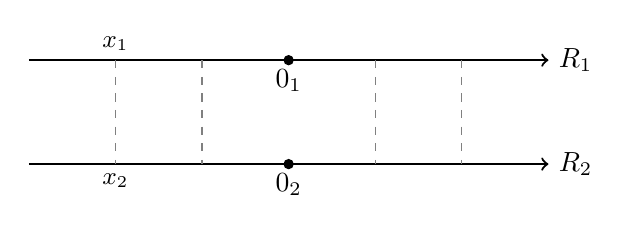
\begin{tikzpicture}[scale=1.1]
    % Recta R1
    \draw[thick, ->] (-3, 1.2) -- (3, 1.2) node[right] {$\mathbb{R}_1$};
    \filldraw (0, 1.2) circle (1.5pt) node[below] {$0_1$};
    
    % Recta R2
    \draw[thick, ->] (-3, 0) -- (3, 0) node[right] {$\mathbb{R}_2$};
    \filldraw (0, 0) circle (1.5pt) node[below] {$0_2$};

    % Líneas de identificación verticales (discontinuas)
    \draw[dashed, gray] (-2, 1.2) -- (-2, 0);
    \draw[dashed, gray] (-1, 1.2) -- (-1, 0);
    \draw[dashed, gray] (1, 1.2) -- (1, 0);
    \draw[dashed, gray] (2, 1.2) -- (2, 0);
    
    \node at (-2, 1.2) [above] {\small $x_1$};
    \node at (-2, 0) [below] {\small $x_2$};
\end{tikzpicture}
\end{center}

Sea $R$ la relación en $X$ definida por
\[x R y \text{ si }
\begin{cases}
x, y \in \mathbb{R}_1 \text{ ó } x, y \in \mathbb{R}_2 \text{ y } x = y \\[1ex]
x \in \mathbb{R}_1, y \in \mathbb{R}_2 \text{ (ó viceversa) y } x = y \in \mathbb{R} \setminus \{0\}
\end{cases} \text{}
\]
\textit{(El $0_1$ no lo identifica con $0_2$)}

\[
X \xrightarrow{\pi} \modulo{X}{R} = \text{ la recta real con el origen desdoblado (como espacio topológico)} 
\]

\begin{center}
\begin{tikzpicture}[scale=1.1]
    % Recta dividida antes del origen
    \draw[thick] (-3, 0) -- (-0.1, 0);
    % Parte derecha después del origen
    \draw[thick, ->] (0.1, 0) -- (3, 0) node[right] {$\mathbb{R}$};
    
    % Origen desdoblado (dos puntos superpuestos en la bifurcación)
    \filldraw[blue] (0, 0.3) circle (1.5pt) node[above] {$0_1$};
    \filldraw[red] (0, -0.3) circle (1.5pt) node[below] {$0_2$};
    
    % Conexiones sutiles hacia el origen desdoblado
    \draw[dashed, blue] (-0.3, 0) -- (0, 0.3) -- (0.3, 0);
    \draw[dashed, red] (-0.3, 0) -- (0, -0.3) -- (0.3, 0);
\end{tikzpicture}
\end{center}

Un subconjunto $W \subseteq \modulo{X}{R}$ es abierto si (es $\iff$):

\begin{enumerate}
    \item $0_1, 0_2 \notin W \implies \begin{array}{l} W \subseteq \mathbb{R}_1 \text{ es abierto} \\ W \subseteq \mathbb{R}_2 \end{array} \iff W \subseteq \mathbb{R} \text{ es abierto } \text{\small(en esta parte no ha cambiado nada)}$.

    \item $\begin{array}{l} 0_1 \in W \\ 0_2 \notin W \end{array} \implies \begin{array}{l} W \subseteq \mathbb{R}_1 \text{ es abierto} \\ W \setminus \{0_1\} \subseteq \mathbb{R}_2 \text{ es abierto} \end{array} \iff W \subseteq \mathbb{R} \text{ es abierto}$.

    \item Ídem para $\begin{array}{l} 0_2 \in W \\ 0_1 \notin W \end{array}$.

    \item $0_1, 0_2 \in W \implies \begin{array}{l} W \subseteq \mathbb{R}_1 \text{ es abierto} \\ W \subseteq \mathbb{R}_2 \end{array} \iff W \subseteq \mathbb{R} \text{ es abierto}$.
\end{enumerate}
\end{ejem}
\chapter{Espacios métricos y pseudométricos}
Sea $X$ un conjunto
\begin{defi} Una \textbf{pseudométrica} $d$ en $X$ es una aplicación de conjuntos
\[
    X \times X \overset{d}{\longrightarrow} \mathbb{R}
\]
verificando las propiedades
\begin{enumerate}
    \item $d(x, y) \ge 0, \, \forall x, y \in X \quad \text{y} \quad d(x, x) = 0, \, \forall x \in X$
    \item Simétrica $d(x, y) = d(y, x), \quad \forall x, y \in X$
    \item Desigualdad triangular $d(x, y) \le d(x, z) + d(z, y), \quad \forall x, y, z \in X$
\end{enumerate}
\end{defi}
\begin{defi} Una \textbf{métrica} ó \textbf{distancia} en $X$ es una pseudométrica $d$ que verifica que:
\[
    d(x, y) = 0 \iff x = y
\] \end{defi}
\begin{ejem} $\mathbb{R}^n$ como conjunto
\[
    d(x, y) = +\sqrt{\sum_{k=1}^n (x_k - y_k)^2} \quad \text{(se prueba que es una distancia)}
\]
donde $x = (x_1, \ldots, x_n) \in \mathbb{R}^n, y = (y_1, \ldots, y_n) \in \mathbb{R}^n$. Entonces $(\mathbb{R}^n, d)$ es un espacio métrico.
\end{ejem}
\begin{ejer}
    Definimos 
$$ \bt \overline{d} : \mathbb{R}^n \times \mathbb{R}^n \rar &  \mathbb{R} \\[-5mm] (x, y) \rarmaps & \overline{d}(x, y) &[-11mm] = \min\{1, d(x, y)\} \et $$
$\overline{d}$ es una métrica en $\mathbb{R}^n$ (se prueba). Es la \textbf{métrica acotada}.
\end{ejer}

\begin{defi}
    Un \textbf{espacio m\'etrico} es una pareja $(X, d)$ donde $X$ es un conjunto y $d$ es una m\'etrica o distancia en $X$.
\end{defi}
\begin{ejem}
    Se tiene que $(X, \overline{d})$ es otro espacio m\'etrico. Es ditsitno porque si $d$ tiene la propiedad de que existen $x,y\in X$ con $d(x,y) > 1$ entonces $\overline{d} \neq d$ como aplicaciones. 
\end{ejem}
\begin{ejem}
Se tiene la distancia suma en $\mathbb{R}^n$ definida por
\[  
    d_{suma}(x, y) := \sum_{i=1}^n |x_i - y_i|, \qquad x = (x_1, \ldots, x_n), y = (y_1, \ldots, y_n) \in \mathbb{R}^n
\]
y en general $d_{suma}\neq d(x,y)$.

Se tiene tambi\'en la m\'etrica del m\'aximo en $\mathbb{R}^n$ definida por
\[
    d_{max}(x, y) \coloneqq \max_{1 \le i \le n} |x_i - y_i|, \qquad x = (x_1, \ldots, x_n), y = (y_1, \ldots, y_n) \in \mathbb{R}^n
\] y tambi\'en $d_{max} \neq d(x,y) \neq d_{suma}$. Tambi\'en se tienen $\overline{d}_{suma}$ y $\overline{d}_{max}$, teni\'endose as\'i 6 m\'etricas distintas en $\mathbb{R}^n$, y como espacios m\'etricos distintos $(\mathbb{R}^n, d), (\mathbb{R}^n, \overline{d}), (\mathbb{R}^n, d_{suma}), (\mathbb{R}^n, \overline{d}_{suma}), (\mathbb{R}^n, d_{max}), (\mathbb{R}^n, \overline{d}_{max})$.
\end{ejem}
\section{Isometr\'ias entre espacios m\'etricos}
 Sean $(X, d)$ y $(Y, d')$ espacios métricos (o pseudométricos)
\begin{defi}
   Una \textbf{isometría} es una aplicación de conjuntos $f: X \longrightarrow Y$ tal que 
    \[
         d(x, x') = d'(f(x), f(x')) \qquad \forall \,  x, x' \in X.
    \]
\end{defi}
\begin{obs}
Si $(X,d)$ es espacio m\'etrico, entonces toda isometr\'ia $f$ es inyectiva, pues si $f(x) = f(x')$ entonces $d(x, x') = d'(f(x), f(x')) = d'(f(x), f(x)) = 0 \implies x = x'$ por ser $d$ una m\'etrica. En cambio, si $(X,d)$ es pseudométrico, $f$ puede no ser inyectiva.
\end{obs}
\begin{obs}
    En alguna literatura se define isometría como aplicación biyectiva que preserva la distancia, pero nosotros no suponemos que sea biyectiva.
\end{obs}
\begin{prop}
    Todo subconjunto $Z \subseteq X$ de un espacio (pseudo)métrico $(X, d)$ es un espacio (pseudo)métrico $(Z, d|_{Z \times Z})$ con la métrica inducida por $d$
    $$\begin{tikzcd}
        X \times X \rar{d} & \bb R \\[-5mm] \arrow[phantom]{u}{\cup} Z \times Z \rar{d|_{Z \times Z}} & \bb R 
    \end{tikzcd}$$
\end{prop}
\begin{defi}
    Si $A \subset (X,d)$ se dice que $A$ es un \textbf{subconjunto acotado} si $d|_{A \times A}: A\times A \longrightarrow \mathbb{R}$ es una aplicaci\'on acotada, es decir, si existe alg\'un $M > 0$ tal que $d(a, a') \le M$ para todo $a, a' \in A$.
\end{defi}
\begin{ejem}
    $(\bb R, d)\supset \bb N$ no es acotado. $(\bb R, \overline{d}) \supset \bb N$ s\'i es acotado.
\end{ejem}
\begin{defi}
    Si $A \subset (X,d)$ espacio m\'etrico se define la distancia de un punto $x \in X$ a un conjunto $A$ como
    $$\bt d_A : X \rar & \bb R \\[-5mm] x \rarmaps & d_A(x) &[-11mm] \coloneqq  \inf \{d(x, a) :  a \in A \} \et$$
\end{defi}
\section{Topolog\'ia asociada a una m\'etrica}
Sea $(X, d)$ un espacio pseudom\'etrico
\begin{defi}
    Se define la \textbf{topolog\'ia $\mc T_d$ asociada a la pseudom\'etrica} $d$ en $X$ por entornos. Dado $x\in X$, una base de entornos de $x$ es $\{B_d(x, \varepsilon)\}_{\varepsilon > 0}$ donde 
    $$B_d(x, \varepsilon) \coloneqq \{y \in X : d(x, y) < \varepsilon\}$$
    que genera la topolog\'ia $\mc T_d$ en $X$.
\end{defi}
As\'i, dado $(X,d)$ espacio pseudom\'etrico, hemos construido $(X, \mc T_d)$.
\begin{ejer}
    Se comprueba que en $(X,\mc T_d)$ las bolas abiertas $B_d(x, \varepsilon)$ son abiertos en $\mc T_d$ y que $\{B_d(x, \varepsilon)\}_{\varepsilon > 0}$ es una base de entornos de $x$. Para probar que son abiertos, se ve que $\forall \, y \in B_d(x, \varepsilon) \, \exists \, \delta_y$ tal que $B_d(y, \delta_y) \subset B_d(x, \varepsilon)$, y es $\delta_y = \varepsilon - d(x, y) > 0$.
\end{ejer}
\begin{defi}
    Se define la \textbf{bola cerrada} de radio $\varepsilon$ centrada en $x$ como $\overline{B}_d(x, \varepsilon) = \{y \in X : d(x, y) \le \varepsilon\}$.
\end{defi}
\begin{ejer}
    Son cerrados. Comprobar que el complementario es abierto.
\end{ejer}
\begin{obs}
    En general, $\overline{B}_d(x, \varepsilon)$ no es el cierre de $B_d(x, \varepsilon)$, aunque $B_d(x, \varepsilon) \subset \overline{B}_d(x, \varepsilon)$.
\end{obs}
\begin{defi}
    Se define la \textbf{esfera} de radio $\varepsilon$ centrada en $x$ como
    $$S_d(x, \varepsilon) = \{y \in X : d(x, y) = \varepsilon\}$$
\end{defi}

De forma que $B_d(x, \varepsilon) \subset \overline{B}_d(x, \varepsilon)$ y $S_d(x, \varepsilon) \subset \overline{B}_d(x, \varepsilon)$, y en m\'etricas usuales (continuas) suele ser la frontera.

¿Podemos construir una topología a partir de una pseudométrica? En general, no.

Esto da lugar a la siguiente definici\'on
\begin{defi}
    Un espacio topol\'ogico se dice que es \textbf{(pseudo)metrizable} si existe una (pseudo)m\'etrica $d$ en $X$ tal que $\mc T_d = \mc T_X$.
\end{defi}

Esta asignaci\'on no es inyectiva, pues distintas pseudom\'etricas pueden generar la misma topolog\'ia.

\begin{ejem}
    Por ejemplo, consideremos $(X,d)$ espacio m\'etrico cualquiera y $\overline{d}$ la m\'etrica acotada, generan la misma topolog\'ia. Como espacios m\'etricos son distintos, $(X, d)$ y $(X, \overline{d})$ pero como espacios topol\'ogicos $(X, \mc T_d) = (X, \mc T_{\overline{d}})$.

    Como con $\{B_d(x,\varepsilon)\}_{0< \varepsilon < 1}$ es base de entornos de $\mc T_d$ y $\{B_{\overline{d}}(x,\varepsilon)\}_{0< \varepsilon < 1}$ es base de entornos de $\mc T_{\overline{d}}$, se verifica que $\{B_d(x,\varepsilon)\}_{0< \varepsilon < 1} = \{B_{\overline{d}} (x,\varepsilon) \}_{0< \varepsilon < 1}$. Esto es porque los entornos son algo local.
\end{ejem}
\begin{obs}
    Esto nos dice que al trabajar a nivel de espacios topol\'ogicos, no podemos distinguir entre $(X,d)$ y $(X,\overline{d})$, y podemos escoger la m\'etrica que nos convenga, acotada o no acotada. En cambio, a nivel de espacios m\'etricos, son distintos.
\end{obs}
\begin{ejem}
    Cerrado y acotado es compacto en $(\bb R,d)$ pero no en otras m\'etricas.
\end{ejem}

En $\mathbb{R}^n$ tenemos las siguientes métricas:
\begin{itemize}
    \item \textbf{Métrica euclídea usual:} 
    \[
    d(x,y) = +\sqrt{\sum_{i=1}^n (x_i - y_i)^2} \rightsquigarrow \overline{d} = \min\{1, d\}
    \]
    \item \textbf{Métrica de la suma ($d_1$):} 
    \[
    d_{\text{sum}}(x,y) = \sum_{i=1}^n |x_i - y_i|
    \]
    \item \textbf{Métrica del máximo ($d_\infty$):} 
    \[
    d_{\text{máx}}(x,y) = \max_{i=1,\dots,n} \{|x_i - y_i|\}
    \]
\end{itemize}

\begin{teo}
$\mathcal{T}_{\overline{d}} = \mathcal{T}_d = \mathcal{T}_{d_{\text{sum}}} = \mathcal{T}_{d_{\text{máx}}}$.
\end{teo}

\begin{dem}
$\mathcal{T}_{\overline{d}} = \mathcal{T}_d$ ya ha sido demostrada previamente.

Observamos las relaciones cuadráticas entre métricas:
\[
\left(d_{\text{sum}}(x,y)\right)^2 = \left(\sum_{i=1}^n |x_i - y_i|\right)^2 = \sum_{i=1}^n |x_i - y_i|^2 + 2\sum_{i < j} |x_i - y_i||x_j - y_j| \ge \sum_{i=1}^n |x_i - y_i|^2 = (d(x,y))^2
\]
\[
\left(d_{\text{máx}}(x,y)\right)^2 = \left(\max_{i=1,\dots,n} \{|x_i - y_i|\}\right)^2 = \max_{i=1,\dots,n} \{|x_i - y_i|^2\} \le \sum_{i=1}^n |x_i - y_i|^2 = (d(x,y))^2
\]

De las desigualdades anteriores se obtiene:
\[
d_{\text{máx}}^2 \le d^2 \le d_{\text{sum}}^2 \implies d_{\text{máx}} \le d \le d_{\text{sum}}
\]

Por otra parte, se satisface $d_{\text{sum}}(x,y) \le n \cdot d_{\text{máx}}(x,y)$, luego:
\[
d_{\text{máx}} \le d \le d_{\text{sum}} \le n \cdot d_{\text{máx}}
\]

Esto implica la inclusión de bolas abiertas entre sí:
\[
B_{d_{\text{sum}}}(x, \varepsilon) \subseteq B_d(x, \varepsilon) \subseteq B_{d_{\text{máx}}}(x, \varepsilon), \quad \forall x \in \mathbb{R}^n, \, \forall \varepsilon > 0.
\]
Por lo tanto:
\[
\mathcal{T}_{d_{\text{máx}}} \subseteq \mathcal{T}_d \subseteq \mathcal{T}_{d_{\text{sum}}}
\]

Si demostramos que $\mathcal{T}_{d_{\text{sum}}} \subseteq \mathcal{T}_{d_{\text{máx}}}$, habremos terminado.

Sea $x \in \mathbb{R}^n$, $\varepsilon > 0$ y la bola $B_{d_{\text{sum}}}(x, \varepsilon)$. Queremos probar que $B_{d_{\text{sum}}}(x, \varepsilon)$ es entorno del punto $x$ en la topología $\mathcal{T}_{d_{\text{máx}}}$, es decir, existe $\delta > 0$ tal que $B_{d_{\text{máx}}}(x, \delta) \subseteq B_{d_{\text{sum}}}(x, \varepsilon)$.

Notemos que
\[
d_{\text{máx}}(x,y) = \max_{i=1,\dots,n} \{|x_i - y_i|\} \ge |x_i - y_i|, \quad \forall i=1,\dots,n
\]
\[
n \cdot d_{\text{máx}}(x,y) \ge \sum_{i=1}^n |x_i - y_i| = d_{\text{sum}}(x,y)
\]

Tomando $\delta = \dfrac{\varepsilon}{n}$, se verifica:
\[
B_{d_{\text{máx}}}\left(x, \frac{\varepsilon}{n}\right) \subseteq B_{d_{\text{sum}}}(x, \varepsilon). 
\]
\end{dem}

% ==============================================================================
\section{Metrizabilidad de la topología producto en $\mathbb{R}^n$}
% ==============================================================================

Consideremos el espacio topológico producto directo $(\mathbb{R}^n, \mathcal{T}_\pi)$.

\begin{teo}
$(\mathbb{R}^n, \mathcal{T}_\pi)$ es metrizable. Además, se verifica que $\mathcal{T}_\pi = \mathcal{T}_d = \mathcal{T}_{\overline{d}} = \mathcal{T}_{d_{\text{sum}}} = \mathcal{T}_{d_{\text{máx}}}$.
\end{teo}

\begin{dem}
Vamos a probar que $\mathcal{T}_\pi = \mathcal{T}_{d_{\text{máx}}}$ (lo que concluye la demostración por el teorema anterior).

\begin{itemize}  \item[$\boxed{\subseteq}$] Sea $U \in \mathcal{T}_\pi$ un abierto básico (basta probarlo para abiertos básicos).
\[
U = U_1 \times U_2 \times \dots \times U_n, \quad U_i \subseteq \mathbb{R} \text{ abierto } \forall i.
\]
Queremos ver que $U$ es $\mathcal{T}_{d_{\text{máx}}}$-abierto, es decir, es entorno de todos sus puntos por la topología $\mathcal{T}_{d_{\text{máx}}}$.

Sea $x = (x_1, \dots, x_n) \in U = U_1 \times \dots \times U_n$. Dado que cada $x_i \in U_i \in \mathcal{T}_d$, existe $\varepsilon_i > 0$ tal que $B_{d_1}(x_i, \varepsilon_i) \subseteq U_i$.

Tomamos $\varepsilon = \min\{\varepsilon_i\}_{i=1}^n > 0$. Se verifica que $x \in B_{d_{\text{máx}}}(x, \varepsilon) \subseteq U$. En efecto, si $y \in B_{d_{\text{máx}}}(x, \varepsilon)$, entonces:
\[
d_{\text{máx}}(x,y) < \varepsilon \le \varepsilon_i \implies |x_i - y_i| < \varepsilon_i \implies y_i \in B_{d_1}(x_i, \varepsilon_i) \subseteq U_i, \quad \forall i=1,\dots,n.
\]
Por lo tanto, $y = (y_1, \dots, y_n) \in U_1 \times \dots \times U_n = U \implies B_{d_{\text{máx}}}(x, \varepsilon) \subseteq U$.

\item[$\boxed{\supseteq}$] Sea $x \in \mathbb{R}^n$, $\varepsilon > 0$ y la bola $B_{d_{\text{máx}}}(x, \varepsilon)$. Tenemos que probar que $B_{d_{\text{máx}}}(x, \varepsilon)$ es entorno del punto $x$ por la topología $\mathcal{T}_\pi$, es decir, que existe un abierto básico $U \in \mathcal{T}_\pi$ tal que $x \in U \subseteq B_{d_{\text{máx}}}(x, \varepsilon)$.

Tomamos $U = (x_1 - \varepsilon, x_1 + \varepsilon) \times \dots \times (x_n - \varepsilon, x_n + \varepsilon) \in \mathcal{T}_\pi$.

Sea $y \in U \implies y_i \in (x_i - \varepsilon, x_i + \varepsilon), \, \forall i \implies |x_i - y_i| < \varepsilon, \, \forall i \implies \max_{i=1,\dots,n}\{|x_i - y_i|\} < \varepsilon$.

Por ende, $d_{\text{máx}}(x,y) < \varepsilon \implies y \in B_{d_{\text{máx}}}(x, \varepsilon) \implies U \subseteq B_{d_{\text{máx}}}(x, \varepsilon)$.\
\end{itemize}
\end{dem}

% ==============================================================================
\section{Metrizabilidad del espacio de sucesiones $(\mathbb{R}^\mathbb{N}, \mathcal{T}_\pi)$}
% ==============================================================================

\begin{teo}
$\mathbb{R}^\mathbb{N} = \prod_{n \in \mathbb{N}} \mathbb{R}$ es el espacio de las sucesiones de números reales. Demostrar que $(\mathbb{R}^\mathbb{N}, \mathcal{T}_\pi)$ es metrizable.
\end{teo}

\begin{dem}
Consideremos la función $D: \mathbb{R}^\mathbb{N} \times \mathbb{R}^\mathbb{N} \longrightarrow \mathbb{R}^+$ definida por:
\[
D(x,y) = \sup_{n \in \mathbb{N}} \left\{ \frac{\overline{d}(x_n, y_n)}{n} \right\} = \sup_{n \in \mathbb{N}} \left\{ \frac{\min\{1, |x_n - y_n|\}}{n} \right\}
\]
donde el supremo existe pues está acotado superiormente por $1$ (dado que $\frac{\overline{d}}{n} \le \frac{1}{n} \le 1$).

Comprobamos que $D$ define una métrica en $\mathbb{R}^\mathbb{N}$. Probamos la desigualdad triangular:
\[
\frac{\overline{d}(x_n, y_n)}{n} \le \frac{\overline{d}(x_n, z_n)}{n} + \frac{\overline{d}(z_n, y_n)}{n}, \quad \forall z \in \mathbb{R}^\mathbb{N}
\]
Tomando supremos a ambos lados sobre $n \ge 1$:
\[
\sup \left\{ \frac{\overline{d}(x_n, y_n)}{n} \right\} \le \sup \left\{ \frac{\overline{d}(x_n, z_n)}{n} + \frac{\overline{d}(z_n, y_n)}{n} \right\} \le \sup \left\{ \frac{\overline{d}(x_n, z_n)}{n} \right\} + \sup \left\{ \frac{\overline{d}(z_n, y_n)}{n} \right\}
\]
luego $D(x,y) \le D(x,z) + D(z,y)$.

\medskip

Falta ver que $\mathcal{T}_\pi = \mathcal{T}_D$. Para ello, probamos la inclusión en ambos sentidos.
\begin{itemize}
\item[$\boxed{\supseteq}$] Queremos probar que para todo $x \in \mathbb{R}^\mathbb{N}$ y $\varepsilon > 0$, existe $U \in \mathcal{T}_\pi$ tal que $x \in U \subseteq B_D(x, \varepsilon)$.

Dado $\varepsilon > 0$, sea $N \in \mathbb{N}$ tal que $\dfrac{1}{N} < \varepsilon$. Tomamos el abierto básico de $\mathcal{T}_\pi$:
\[
U = B_{\overline{d}}\left(x_1, \frac{\varepsilon}{N}\right) \times \dots \times B_{\overline{d}}\left(x_N, \frac{\varepsilon}{N}\right) \times \mathbb{R} \times \mathbb{R} \times \dots \in \mathcal{T}_\pi
\]
Si $y \in U$, entonces para $n \le N$ se tiene $\overline{d}(x_n, y_n) < \dfrac{\varepsilon}{N} \implies \dfrac{\overline{d}(x_n, y_n)}{n} \le \overline{d}(x_n, y_n) < \dfrac{\varepsilon}{N} < \varepsilon$. 

Para $n > N$, se tiene $\dfrac{\overline{d}(x_n, y_n)}{n} \le \dfrac{1}{n} < \dfrac{1}{N} < \varepsilon$. 

Por consiguiente, $D(x,y) = \sup_{n \ge 1} \left\{ \frac{\overline{d}(x_n, y_n)}{n} \right\} < \varepsilon \Rightarrow y \in B_D(x, \varepsilon)$, lo que demuestra que $U \subseteq B_D(x, \varepsilon)$.

\item[$\boxed{\subseteq}$] Basta probarlo para la subbase de $\mathcal{T}_\pi$, dada por los subconjuntos del tipo:
\[
(x_n - \varepsilon, x_n + \varepsilon) \times \prod_{k \neq n} \mathbb{R} \subseteq \mathbb{R}^\mathbb{N}
\]
al probar la inclusión para elementos subbásicos, queda probada para toda la topología $\mathcal{T}_\pi \subseteq \mathcal{T}_D$. 
\end{itemize}
\end{dem}
\begin{tikzpicture}[
    scale=1.0,
    font=\small,
    >=Stealth,
    caja/.style={draw=blue!70!black, fill=blue!8, rounded corners=2pt, thick},
    sucesion/.style={draw=red!75!black, thick},
    punto/.style={fill=red!75!black, circle, inner sep=1.6pt},
    puntox/.style={fill=blue!70!black, circle, inner sep=1.9pt},
    etiqueta/.style={inner sep=1.2pt}
]

% --- Ejes / Líneas verticales de coordenadas ---
\foreach \x/\etq in {0/1, 1.9/2, 3.8/3, 6.3/N, 8.6/N+1, 10.6/N+2, 12.6/N+3} {
    \draw[gray!45, dashed] (\x, -2.2) -- (\x, 2.2);
    \node[above, etiqueta] at (\x, 2.3) {$n = \etq$};
}

% --- Puntos suspensivos entre 3 y N, y después de N+3 ---
\node[etiqueta] at (5.05, 2.45) {$\cdots$};
\node[etiqueta] at (5.05, 0) {$\cdots$};
\node[etiqueta] at (13.6, 2.45) {$\cdots$};
\node[etiqueta] at (13.6, 0) {$\cdots$};

% --- Muro / Frontera en N (separado de n=N y n=N+1) ---
\draw[orange!85!black, ultra thick, dashed] (7.45, -2.5) -- (7.45, 2.95);
\node[orange!85!black, fill=white, draw=orange!60!black, rounded corners=2pt, inner sep=2.5pt, font=\footnotesize\bfseries] at (7.45, 3.15) {Frontera $N$ ($\frac{1}{N} < \varepsilon$)};

% --- Cajas de control en Zona 1 (n <= N) con etiquetas de bolas limpias ---
\foreach \x/\idx in {0/1, 1.9/2, 3.8/3, 6.3/N} {
    \draw[caja] (\x-0.45, -0.75) rectangle (\x+0.45, 0.75);
    \node[blue!70!black, etiqueta, font=\scriptsize, below] at (\x, -0.82) {$B_{\bar{d}}\!\left(x_{\idx}, \frac{\varepsilon}{N}\right)$};
}

% --- Rectas completas R en Zona 2 (n > N) ---
\foreach \x in {8.6, 10.6, 12.6} {
    \draw[teal!70!black, very thick] (\x, -1.9) -- (\x, 1.9);
    \node[teal!70!black, etiqueta, font=\footnotesize, below] at (\x, -1.98) {$\mathbb{R}$};
}

% --- Sucesión central x (línea horizontal azul en y=0) ---
\draw[blue!70!black, thick] (-0.5, 0) -- (4.5, 0);
\draw[blue!70!black, thick] (5.6, 0) -- (13.1, 0);
\foreach \x/\idx in {0/1, 1.9/2, 3.8/3, 6.3/N, 8.6/N+1, 10.6/N+2, 12.6/N+3} {
    \node[puntox] at (\x, 0) {};
    \node[blue!70!black, etiqueta, font=\scriptsize, above right=1.5pt] at (\x, 0) {$x_{\idx}$};
}

% --- Sucesión y \in U (línea roja) ---
\coordinate (y1) at (0, 0.42);
\coordinate (y2) at (1.9, -0.45);
\coordinate (y3) at (3.8, 0.35);
\coordinate (yN) at (6.3, -0.35);
\coordinate (yN1) at (8.6, 1.5);
\coordinate (yN2) at (10.6, -1.55);
\coordinate (yN3) at (12.6, 1.25);

\draw[sucesion] (y1) -- (y2) -- (y3) -- (4.5, 0.15);
\draw[sucesion] (5.6, -0.15) -- (yN) -- (yN1) -- (yN2) -- (yN3);

\foreach \pt in {y1, y2, y3, yN, yN1, yN2, yN3} {
    \node[punto] at (\pt) {};
}
\node[red!75!black, etiqueta, font=\scriptsize, above left=2pt] at (y1) {$y_1$};
\node[red!75!black, etiqueta, font=\scriptsize, above left=2pt] at (y2) {$y_2$};
\node[red!75!black, etiqueta, font=\scriptsize, above left=2pt] at (y3) {$y_3$};
\node[red!75!black, etiqueta, font=\scriptsize, above left=2pt] at (yN) {$y_N$};
\node[red!75!black, etiqueta, font=\scriptsize, above left=2pt] at (yN1) {$y_{N+1}$};
\node[red!75!black, etiqueta, font=\scriptsize, below right=2pt] at (yN2) {$y_{N+2}$};
\node[red!75!black, etiqueta, font=\scriptsize, above left=2pt] at (yN3) {$y_{N+3}$};

% --- Llaves inferiores explicativas ---
\draw[decorate, decoration={brace, amplitude=6pt, mirror}, thick, blue!70!black]
    (-0.5, -2.75) -- (7.25, -2.75)
    node[midway, below=8pt, align=center, font=\footnotesize] {
        \textbf{ZONA 1 ($n \le N$): Controlada por $U$}\\
        $\frac{\bar{d}(x_n, y_n)}{n} \le \bar{d}(x_n, y_n) < \frac{\varepsilon}{N} < \varepsilon$
    };

\draw[decorate, decoration={brace, amplitude=6pt, mirror}, thick, teal!70!black]
    (7.65, -2.75) -- (13.1, -2.75)
    node[midway, below=8pt, align=center, font=\footnotesize] {
        \textbf{ZONA 2 ($n > N$): Libre (todo $\mathbb{R}$)}\\
        $\frac{\bar{d}(x_n, y_n)}{n} \le \frac{1}{n} < \frac{1}{N} < \varepsilon$
    };

\end{tikzpicture}


\section{Axiomas de numerabilidad}
Sea $X$ un espacio topol\'ogico
\begin{defi}
   Se dice que $X$ es \textbf{primero numerable} o $1AN$ si cada punto $x \in X$ tiene una base numerable de entornos $\{U_n\}_{n \in \mathbb{N}}$. Adem\'as se pueden considerar entornos abiertos.
\end{defi}
\begin{ejem}
Todo espacio métrico cumple el primer axioma de numerabilidad, pues las bolas abiertas 
{$\displaystyle B_{n}=B(x,\nicefrac{1}{n})$} forman una base de entornos para el punto $ x\in X$. 

La recta cofinita, $\displaystyle (\mathbb {R} ,\mathcal{T} _{cof})$, no es primero numerable.
\end{ejem}
\begin{defi}
    Se dice que $X$ es \textbf{segundo numerable} o $2AN$ si tiene una base numerable $\{U_n\}_{n \in \mathbb{N}}$ de abiertos de la topología $\mathcal{T}_X$.
\end{defi}
\begin{ejem}
    El espacio de Sorgenfrey no es $2AN$, aunque sí es $1AN$.
\end{ejem}
\begin{defi}
    Se dice que $X$ es \textbf{separable} si existe un subconjunto $A \subseteq X$ numerable y denso en $X$, es decir, $\overline{A} = X$.
\end{defi}
\begin{ejem}
    El espacio euclídeo $\mathbb {R} ^{n}$ con su topología usual es $2AN$. Aunque la base formada por las bolas abiertas no es numerable, podemos encontrar una base que sí lo es: la formada por las bolas de radio racional y cuyo centro tenga coordenadas racionales.

La táctica anterior puede repetirse en un espacio métrico separable (i.e. que contenga un subconjunto denso numerable $A$). Como base basta escoger de nuevo las bolas de radio racional centradas en $A$.
\end{ejem}
\begin{prop}
    Se verifica que 
    \begin{enumerate}
        \item $2AN \Rightarrow 1AN$.
        \item $2AN$ y separable $\Rightarrow \, 1AN$.
        \item Si $(X,d)$ es un espacio pseudom\'etrico, entonces es $1AN$.
    \end{enumerate} 
\end{prop}
\begin{dem}
    \begin{enumerate}
        \item \,
        \item Sea $D = \{x_n :n \in \bb N\}$ un subconjunto numerable y denso en $X$. Sea $\{V_{x_n}^m\}_{m \in \bb N}$ una base numerable de entornos abiertos de cada $x_n$. Entonces $\{V_{x_n}^m: x_n \in D, \, m \in \bb N\}$ es una base de abiertos de $X$.
        \item $\{ B_d(x_n, \nicefrac{1}{m}) \}_{m \in \bb N}$ es una base numerable de abiertos de $X$.
    \end{enumerate}
\end{dem}
\begin{ejem} $(\bb R,d)$ es m\'etrico, luego $\bb R$ es $1AN$. Adem\'as, $\bb R$ es separable, pues $\bb Q$ es denso en $\bb R$ y numerable. Por lo tanto, $(\bb R, d)$ es $2AN$.
\end{ejem}
\begin{teo}
    [de Metrizaci\'on de Urysohn] Sea $X$ un espacio topol\'ogico regular, $T_0$ y $2AN$, entonces $X$ es metrizable.
\end{teo}
\begin{lem}
Regular + $2AN$ $\Rightarrow$ Normal.
\end{lem}
\begin{dem}
    Sean $C,C'$ cerrados en $X$ disjuntos por regularidad. Sea $x\in C, \, x\nin C' \Rightarrow \exists \, U_x$ b\'asicos de la familia numerable tal que $\overline{U}_x \cap C = \emptyset$. Sean $C \subset U = \bigcup_{n \in \bb N} U_n$ abierto y $C' \subset U' = \bigcup_{m \in \bb N} U_m'$ abierto, pero no aseguramos que sea disjuntos. Entonces ``achicamos'' de forma que 
    $$\hat U_n \coloneqq U_n - \bigcup_{m=1}^{n} \overline{U}'_m \text{ es abierto}$$
    $$\hat U_n' \coloneqq U_n' - \bigcup_{m=1}^{n} \overline{U}_m \text{ es abierto}$$
    y as\'i $C\subset \bigcup_{n \in \bb N} \hat U_n = \hat U$ y $C' \subset \bigcup_{m \in \bb N} \hat U_m' = \hat U'$ y adem\'as ahora s\'i $\hat U\cap \hat U' =\emptyset$. \textcolor{red}{Ejercicio}. 
\end{dem}
\begin{obs}
    Gracias a esto se puede incluir cualquier $X$ m\'etrico en el cubo de Hilbert $[0,1]^{\bb N} = \prod_{n=1}^{\infty} [0,1]$, que es un espacio m\'etrico.
\end{obs}

\section{Propiedades de los espacios metrizables} \footnote{Ejercicios 4}
Sea $(X,\mc T_d)$ con $d$ pseudom\'etrica.

\begin{propi} $d(x,y) = 0\iff \overline{\{x\}} = \overline{\{y\}}$
\end{propi}
\begin{dem} Se tiene la cadena de implicaciones
    $$d(x,y)=0 \iff \, \forall \,  \varepsilon >0, d(x,y) < \varepsilon  \iff \begin{cases} B_d(x,\varepsilon) \ni y \\[-3mm]  \text{ y } \\[-3mm] B_d(y,\varepsilon) \ni x 
    \end{cases}  \iff \begin{cases}
        x\in \overline{\{y\}} \\[-3mm] \text{ y } \\[-3mm] y \in \overline{\{x\}}
    \end{cases} \iff \overline{\{x\}} = \overline{\{y\}}$$
    pero esto no es equivalente a que $x=y$, pues $d$ no es m\'etrica. 
    \end{dem}
\begin{ejer}[123]
    La siguientes condiciones son equivalentes:
    \begin{enumerate}
        \item $X$ es $T_0$
        \item $X$ es $T_2$
        \item $d$ es una m\'etrica. 
    \end{enumerate}
\end{ejer}
\begin{dem}
    1) $\iff$ 3) $\Leftarrow)$ Es general.

    1) $\iff$ 3) $(d(x,y) = 0 \iff \overline{\{x\}} = \overline{\{y\}} \overset{T_0}{\iff} x=y) \iff d $ es m\'etrica.

    3) $\iff$ 2) Si $x\neq y$, $d(x,y) = \varepsilon >0$, entonces $B_d(x, \nicefrac{\varepsilon}{2}) \cap B_d(y, \nicefrac{\varepsilon}{2}) = \emptyset$.
\end{dem}
Varios de los conceptos topol\'ogicos en un espacio metrizable se pueden decir con sucesiones.
\begin{ejer}
[122] $f: X \longrightarrow (Y, \mc T)$ es continua $\iff$ para toda sucesi\'on $\{x_n\}$ de $X$ con $\{x_n\} \to x \in X$ se verifica que $\{f(x_n)\} \to f(x)$. 
\end{ejer}
\begin{sol}
    \begin{itemize}
        \item[$\Rightarrow)$] Se verifica en general, para todo espacio topol\'ogico.
        \item[$\Leftarrow)$] Sea $C \subset Y$ cerrado, veamos que $f^{-1}(C) \subset X$ es cerrado. $f^{-1}(C)$ es cerrado $\iff f^{-1}(C) = \overline{f^{-1}(C)} \iff \forall \, x\in \overline{f^{-1}(C)} \Rightarrow x\in f^{-1}(C)$. Si $x\in \overline{f^{-1}(C)} $ entonces $\exists \{x_n \} \subset f^{-1}(C)$ tal que $\{x_n\} \to x$ por 1). Por las hip\'otesis, $\{f(x_n)\} \to f(x)$. Pero $\{f(x_n)\} \subset C$ por lo que $f(x) \in \overline{C} = C \Rightarrow x \in f^{-1}(C)$. 
        \end{itemize}
\end{sol}
\begin{obs}
    Si $(X,\mc T_d)$ e $(Y, \mc T_{d'})$, entonces $f:X \longrightarrow Y$ es continua $\iff$ para cada $x\in X$ y $\varepsilon >0$ existe un $\delta(x, \varepsilon) \in \bb R^+$ tal que para todo $x' \in X$ con $d(x,x') < \delta \Rightarrow d'(f(x),f(x'))< \varepsilon \iff B_d(x, \delta) \subset f^{-1} (B_{d'}(f(x), \varepsilon))$. 
    (Se fija $x$ para hacerlo por entornos)
\end{obs}
\begin{defi}
$f: X \longrightarrow Y$ es \textbf{uniformemente continua} si es continua y $\delta(x, \varepsilon) = \delta(\varepsilon) \, \forall \, x\in X$, si y solo si, $\forall \varepsilon >0$ existe $\delta(\varepsilon)>0$ tal que $\forall \, x, x'\in X$ con $d(x,x')< \delta$ entonces $d'(f(x),f(x'))< \varepsilon$.  
\end{defi}


Sea $(X,\mc T_d)$ metrizable
\begin{prop}
    $d: X \times X \longrightarrow \bb R$ es continua. 
\end{prop}
\begin{dem}
    Al ser metrizables trabajamos con entornos. Tenemos
    $$\bt d: (X\times X, \mc T_{\pi}) \rar & (\bb R, \mc T_{d_1}) \\[-5mm] (x,y) \rarmaps & d(x,y) \et$$
    escogemos $B_{d_1}(d(x,y), \varepsilon) = (d(x,y)- \varepsilon , d(x,y)+ \varepsilon)$, y 
    $$f^{-1}(B_{d_1}(d(x,y), \varepsilon)) \supset B_{d}(y, \nicefrac{\varepsilon}{2}) \times B_{d}(x, \nicefrac{\varepsilon}{2}) \ni (x,y), (x',y')$$
    por ser los abiertos b\'asicos productos de bolas, y as\'i $|d(x,y) - d(x',y')|< \varepsilon$ usando la desigualdad triangular.
\end{dem}
\begin{ejer}
    $\{x_n\} \to x \iff \displaystyle \lim_{n\to \infty} d(x,x_n)=0$
\end{ejer}
\begin{ejer}
    [126] Sea $A\subseteq X$ un subconjunto de un espacio m\'etrico $(X,d)$. Probar:
    \begin{enumerate}[a)]
        \item $x \in \overline{A} \iff $ existe una sucesi\'on $\{x_n\}_{n\in \bb N} \subseteq A$ tal que $\lim_{n\to \infty} d(x,x_n)=0$
        \item $\overline{A} = \{x\in X: \text{ existe una sucesi\'on } \{x_n\} \subset A \text{ tal que } \{x_n\} \to x \}$. 
        \item $\overline{A} = \{x\in X : d(x,A) = 0\}$ sabiendo que $d_A(x) = d(A,x) = \inf\{d(x,a): a\in A\}$
        \item La aplicaci\'on $d_A : X \to \bb R$ definida por $d_A(x) = d(x,A)$ es una aplicaci\'on (uniformemente) continua.
    \end{enumerate}
\end{ejer}
\begin{sol} \,
    \begin{enumerate}[a)]
        \item \textcolor{red}{Equivalencia con b)}
        \item \begin{itemize}
        \item[$\boxed{\supseteq}$] Se verifica en general. Si $\{x_n\} \to x \Rightarrow x\in \overline{\{x_n\}}_{n \in \bb N} \subset \overline{A}$.
        \item[$\boxed{\subseteq}$] $x\in \overline{A}$. Para cada $n\in \bb N$, $B_d(x,\nicefrac{1}{n}) \cap A \neq \emptyset$. Sea $x\in B_d(x,\nicefrac{1}{n}) \cap A $, $\{x_n\} \subset A$ y se comprueba que $\{x_n\} \to x$ por como se comportan las bolas $B_d(x,\nicefrac{1}{n})$. 
        \end{itemize}
        \item \begin{itemize}
        \item[$\boxed{\supseteq}$] Sea $x\in \{\dots\}$, $d(x,A)=0$, por ser el \'infimo de las distancias, esto es que $\forall \, \varepsilon >0$ existe $a_{\varepsilon} \in A$ tal que $d(x,a_{\varepsilon})< \varepsilon \Rightarrow a_{\varepsilon} \in B_d(x, \varepsilon) \cap A \neq \emptyset \Rightarrow x\in \overline{A}$. 
        \item[$\boxed{\subseteq}$] \textcolor{red}{Ejercicio}
        \end{itemize}
        Sea $\varepsilon >0$, buscamos $\delta > 0$ tal que si $d(x,y)< \delta \Rightarrow |d(x,H) - d(y, H)| < \varepsilon$. Podemos tomar $\varepsilon = \delta$ por ser $|d(x,A) - d(y,A)| \leq d(x,y)$, o equivalentemente,
        $$ \begin{cases}
            d(x,A) - d(y,A) \leq d(x,y)  \\ d(y,A) -  d(x,A)  \leq d(x,y) 
        \end{cases}$$
    y por la simetr\'ia de $d$ basta con demostrar una. 

    Sea $\varepsilon> 0$, como $d(x,A) = \inf\{ d(x,a) : a\in A\}$ existe $a_{\varepsilon}$ tal que $d(x, a_{\varepsilon}) \leq d(x, A) + \varepsilon$,
    $$d(y,a_{\varepsilon}) \leq d(x,y) + d(x, a_{\varepsilon}) \leq d(x,y) + d(x,a_{\varepsilon}) + \varepsilon $$
    $$ \Rightarrow d(y,A) - d(x,A) \leq d(x,y) +\varepsilon$$
    \end{enumerate}
\end{sol}
\begin{ejer}
    Si $(X, \mc T_d)$ es metrizable entonces $X$ es normal (completamente normal). 
\end{ejer}
\begin{ejer}[120]
Demuéstrese que todo espacio métrico es normal. Más concretamente, todo espacio métrico es completamente normal, es decir, si $A$ y $B$ son dos subconjuntos tales que $\overline{A}\cap B = \emptyset$ y $A \cap \overline{B} = \emptyset$, entonces $A$ y $B$ est\'an separados, i.e. existen abiertos disjuntos $U$ y $V$ tales que $A \subset U$ y $B \subset V$.
\end{ejer}
\begin{dem}
    $d_A$ y $d_B$ son continuas, y definimos 
    $$\bt X \rar{d_{A,B}} & \bb R \\[-5mm] x \rarmaps & d(x,A) - d(x,B) \et$$
    y consideramos $d_{AB}^{-1}(0, \infty)$ y $d_{AB}^{-1}(-\infty,0)$ abiertos de $X$. Por ser $d(x, A)=0$ si $x\in A$ y la caracterizaci\'on de los cierres, $d(x,B) > 0 \iff -d(x,B)<0 $ de forma que va a parar a $(-\infty, 0)$ y as\'i $A \subset d_{AB}^{-1}(-\infty,0)$, y de la misma forma $B \subset d_{AB}^{-1}(0,\infty)$,y as\'i
    $$d_{AB}^{-1}(0,\infty) \cap d_{AB}^{-1}(-\infty,0) = \emptyset$$
\end{dem} \cleardoublepage % ==============================================================================
\chapter{Espacios conexos} \justifying
% ==============================================================================
\section{Espacios conexos y separaciones}

Sea $X$ un espacio topológico.

\begin{defi}
Una \textbf{separación} de $X$ es una pareja $(A, B)$ tal que $A, B \subseteq X$ son abiertos (o cerrados) no vacíos verificando que $X = A \cup B$ y $A \cap B = \emptyset$. Es decir, $A$ y $B$ son complementarios.
\end{defi}

\begin{ejem}
$(\emptyset, X)$ es una separación de $X$, denominada la \textbf{separación trivial}.
\end{ejem}

\begin{defi}
Un espacio topológico $X$ es \textbf{conexo} si no admite separaciones no triviales. Es decir, si $X = A \cup B$ con $(A, B)$ una separación, entonces $A = X$ y $B = \emptyset$ (o viceversa).
\end{defi}

\begin{defi}
Un \textbf{subespacio topológico $Y \subseteq X$} es \textbf{conexo} si lo es como espacio topológico con la topología heredada $(Y, \mathcal{T}_X|_Y)$.
\end{defi}

\begin{obs}
Sean $Y \subseteq Z \subseteq X$ subespacios, $Y \subseteq Z$ es subespacio conexo $\Rightarrow Y \subseteq X$ es subespacio conexo. La noción de conjunto conexo es \textbf{absoluta}, no depende del espacio ambiente (aunque la topología sí depende del ambiente, la conexi\'on se preserva: $\mathcal{T}_Z|_Y = \mathcal{T}_X|_Y$).
\end{obs}

\begin{prop}
Sea $Y \subseteq X$ un subespacio. Si $Y = A \cup B$ con $A \cap B = \emptyset$ siendo $A, B$ abiertos (o cerrados) en $Y$, entonces existen $U, V \subseteq X$ abiertos (o cerrados) en $X$ tales que:
\[
A = U \cap Y, \quad B = V \cap Y \quad (\text{o bien } A = \overline{A}^X \cap Y, \, B = \overline{B}^X \cap Y)
\]
De forma que $Y \subseteq U \cup V$ y $(U \cap V) \cap Y = \emptyset = (U \cap Y) \cap (V \cap Y)$.

Si se verifica que $Y \subseteq U$ o $Y \subseteq V \implies Y \subseteq U \cap Y$ o $Y \subseteq V \cap Y \implies A = Y$ o $B = Y$, haciendo que uno de los dos conjuntos sea el total y el otro el vacío.
\end{prop}

\begin{ejem}[No Conexidad de $\mathbb{Q}$]
En $(\mathbb{R}, \mathcal{T}_d)$, consideremos el subespacio $\mathbb{Q} \subset \mathbb{R}$. Sea $c \in \mathbb{I} = \mathbb{R} \setminus \mathbb{Q}$ un número irracional. Los conjuntos:
\[
((-\infty, c) \cap \mathbb{Q}) = A \neq \emptyset, \quad ((c, \infty) \cap \mathbb{Q}) = B \neq \emptyset
\]
definen una separación no trivial de $\mathbb{Q}$, puesto que $\mathbb{Q} = A \cup B$ y $A \cap B = \emptyset$, concluyendo que \textbf{$\mathbb{Q}$ no es conexo}.
\end{ejem}

\begin{obs}
$\mathbb{R}$ sí es conexo (se probará a continuación). Un espacio conexo puede contener subespacios conexos y no conexos (por ejemplo, $[0, 1] \subset (\mathbb{R}, \mathcal{T}_d)$ es conexo, mientras que $[0, 1] \cup [2, 3] \subset \mathbb{R}$ no es conexo). Idem para espacios no conexos.
\end{obs}

% ==============================================================================
\section{Conexi\'on en $\bb R$}
% ==============================================================================

\begin{prop}
El intervalo $[0, 1] \subset \mathbb{R}$ es conexo (con la topología heredada de la usual $\mathcal{T}_d$).
\end{prop}

\begin{dem}
Para demostrarlo, supongamos que $[0, 1]$ admite una separación no trivial. Es decir, existen $U, V \subseteq \mathbb{R}$ abiertos en $\mathbb{R}$ tales que:
\[
[0, 1] \subseteq U \cup V, \quad U \cap V \cap [0, 1] = \emptyset, \quad U \cap [0, 1] \neq \emptyset, \quad V \cap [0, 1] \neq \emptyset.
\]
Supongamos sin pérdida de generalidad que $0 \in U$ (luego $0 \notin V$). Como $U$ es abierto en $\mathbb{R}$, existe $\varepsilon > 0$ tal que $[0, \varepsilon) \subseteq U$.

Consideremos el conjunto:
\[
T = \{ x \in [0, 1] : [0, x] \subseteq U \} \neq \emptyset.
\]
$T$ es un conjunto de números reales no vacío (pues $0 \in T$) totalmente ordenado y acotado superiormente por $1$. Por el axioma del supremo en $\mathbb{R}$, existe $r = \sup T \in [0, 1]$. Estudiemos la pertenencia de $r$:

\begin{itemize}
    \item Si $r \in U$: Como $U$ es abierto en $\mathbb{R}$, existe $\varepsilon' > 0$ tal que $[r, r + \varepsilon') \subseteq U$. Como $r = \sup T$, existe algún $x \in T$ cercano a $r$, lo que implica $[0, r + \varepsilon') \subseteq U$, de donde $r + \varepsilon' \in T$, contradiciendo que $r = \sup T$.
    \item Si $r \in V$: Como $V$ es abierto en $\mathbb{R}$, existe $\varepsilon'' > 0$ tal que $(r - \varepsilon'', r] \subseteq V$. De nuevo por ser $r = \sup T$, existiría un elemento $x \in T$ tal que $x > r - \varepsilon''$, lo que implicaría que $[0, x] \subseteq U$, resultando en una intersección no vacía de $U$ y $V$ en $[0, 1]$, lo cual es una contradicción.
    \item Si $r=1\Rightarrow r\in U$.
\end{itemize}

Por lo tanto, $[0,1]\subset U$ o $[0,1] \subset V$ la separación no trivial no puede existir, de modo que $[0, 1]$ es conexo.
\end{dem}

\begin{prop}
Todos los intervalos de la forma $[a, b]$, $(a, b)$ y $[a, b)$ son conexos en $\mathbb{R}$.
\end{prop}

\begin{dem}
Se sabe que $[0, 1] \simeq [a, b]$ son homeomorfos mediante una aplicación lineal. Dado que la conexi\'on es una propiedad topológica conservada por homeomorfismos, el intervalo $[a, b]$ es conexo.

Para intervalos generales $Y = [a, b]$, $(a, b)$ o $[a, b)$, si suponemos que $Y \subseteq U \cup V$ es una separación no trivial con $U \cap V \cap Y = \emptyset$, basta tomar un subintervalo cerrado $[c, d] \subset Y$. Como $[c, d]$ es conexo, debe cumplirse $[c, d] \subseteq U$ o $[c, d] \subseteq V$ de manera excluyente, obteniéndose por extensión que $Y$ es conexo.
\end{dem}

\begin{teo}
La recta real $\mathbb{R}$ es conexa.
\end{teo}

\begin{dem}
Se ha demostrado previamente que $(0, 1) \simeq \mathbb{R}$ son homeomorfos. Al ser $(0, 1)$ un intervalo conexo y preservarse la conexi\'on por homeomorfismos, concluimos que $\mathbb{R}$ es un espacio conexo.
\end{dem}

\begin{defi}
Un subconjunto $I \subseteq \mathbb{R}$ es un \textbf{intervalo} si para todo $c, d \in I$ con $c < d$, se satisface que $[c, d] \subseteq I$.
\end{defi}

\begin{prop}
Los únicos subespacios conexos de $\mathbb{R}$ son los intervalos.
\end{prop}

\begin{dem}
Falta demostrar que los intervalos son los \emph{únicos} subespacios conexos de $\mathbb{R}$.

Sea $Y \subseteq \mathbb{R}$ un subespacio conexo. Vamos a probar que $Y$ debe ser un intervalo. Sean $c, d \in Y$ con $c < d$. Queremos ver que $[c, d] \subseteq Y$.

Supongamos por reducción al absurdo que no es un intervalo. Entonces existe algún punto $z \in \mathbb{R}$ tal que $c < z < d$ con $z \notin Y$. 

Consideremos los conjuntos abiertos en $\mathbb{R}$:
\[
U = (-\infty, z), \quad V = (z, \infty)
\]
Notemos que $Y \subseteq U \cup V = (-\infty, z) \cup (z, \infty)$ ya que $z \notin Y$. Además por ser $Y$ conexo
\[
c \in U \cap Y \implies U \cap Y \neq \emptyset
\]
\[
d \in V \cap Y \implies V \cap Y \neq \emptyset
\]
\[
(U \cap Y) \cap (V \cap Y) = (U \cap V) \cap Y = \emptyset \cap Y = \emptyset
\]
Por lo tanto, $(U \cap Y, V \cap Y)$ constituye una separación no trivial del subespacio $Y$, lo cual contradice la hipótesis de que $Y$ es conexo.

Concluimos que $Y$ debe ser un intervalo.
\end{dem}
\section{Propiedades}
\begin{prop}
    Sea $Y \subset X$ subespacio topol\'ogico conexo y $(A,B)$ separaci\'on de $X$. Entonces $Y \subset A$ \'o $Y \subset B$. Es decir, que si $Y \subset X = A\sqcup B$ ($\sqcup$ como conjuntos), entonces $Y \subset A$ \'o $Y\subset B$
\end{prop}
\begin{dem}
    $Y = (Y\cap A ) \cup (Y \cap B)$ es una separaci\'on $Y$, que es conexo, y $Y\cap A $ es abierto y $Y\cap B$ es abierto, entonces $Y\cap A = Y$ \'o $Y\cap B = Y$, entonces $Y \subset A$ \'o $Y\subset B$.  
\end{dem}
\begin{prop}
    Si $A,B \subset X$ subconjunto con $A \cup B = X$ y $\overline{A}\cap B = \overline{B}\cap A = \emptyset$ entonces $(A,B)$ es separaci\'on de $X$.
\end{prop}
\begin{dem}
    Como $A\subset \overline{A}$ autom\'aticamente $A \cap B = \emptyset$. Veamos que son cerrados. Como $\overline{A} = \bar A \cap X = \bar A \cap (A\cup B) = (\bar A \cap A) \cup (\bar A \cap B) = A \cup \emptyset = A$. De la misma forma con $B$, y como ambos son cerrados, es una separaci\'on.
\end{dem}
\begin{cor}
Si $X$ es conexo, entonces no existen subconjuntos $A,B \subset X$ con $A \cup B = X$ y $\bar A \cap B = \bar B \cap A = \emptyset$.
\end{cor}

Sea $X$ espacio topol\'ogico y $\{X_i \subset X\}_{i \in I}$ subespacios conexos.
\begin{ejer}
    Se verifica que $\bigcup X_i$ es conexo si $\bigcap X_i \neq \emptyset$. $\bigcup X_i$ es conexo si para todo $i, j\in I$ $X_i \cap X_j \neq \emptyset$. La segunda implica la primera. 
\end{ejer}
Demostraremos la primera
\begin{dem}
    $\bigcup X_i \subset A \cup B$ con $A,B$ abiertos, $A\cap B \cap (\bigcup X_i) = \emptyset$ lo que da lugar a una separaci\'on. Para cada $j\in I$, $X_j \subset \bigcup X_i \bigcup A \cup B$ y como es conexo y tiene separaci\'on, $X_j \subset A$ \'o $X_j \subset B$. 

    Sea $x_o \in \bigcap X_i \neq \emptyset \Rightarrow x_o \in X_i\subset A \cup B \, \forall i$ por tanto $x_o \in A$ \'o $x_o \in B$. Supongamos que $x_o \in A \Rightarrow x_o \nin B$, entonces si para alg\'un $j\in I$, $x_o \in X_j \in B$, como $x_o \in X_i \forall i$, $x_o \in B$, contradicci\'on con $x_o \nin B$, luego $X_j \subset A \forall \, j\in I$ por lo que $\bigcup X_j \subset A$. 
\end{dem}
\begin{prop}
    Sea $Y \subset X$ subespacio conexo. Para todo $Z\subset X$ con $Y\subset Z \subset \overline{Y}$ se verifica que $Z$ es conexo. En particular, si $Y$ es conexo $\Rightarrow \overline{Y}$ es conexo.
\end{prop}
\begin{dem}
    Sea $(A,B)$ una separaci\'on de $Z$, $Z = A\cup B$ y $A\cap B=\emptyset$. Supongamos $A$ y $B$ cerrados de $Z$, y $A = \overline{A} \cap Z$ y $B = \overline{B}\cap Z$. 
    
    $Y \subset Z = A\cup B$ y como $Y$ es conexo por la primera proposici\'on, $Y \subset A$ \'o $Y \subset B\Rightarrow \overline{Y} \subset \overline{A}$ \'o $\overline{Y} \subset \overline{B}$. Entonces al cortar con $Z$, $\overline{Y}\cap Z \subset \overline{A} \cap Z$ que es $Z \subset A \Rightarrow Z=A$ \'o de la misma forma $Z=B$.  
\end{dem}
\begin{prop}
    Sean $X,Y$ espacios topol\'ogicos, $f: X \longrightarrow Y$ aplicaci\'on continua. Si $A\subset X$ es subespacio conexo, entonces $f(A) \subset Y$ es un subespacio conexo. 

    En particular, si $X$ es conexo, entonces $\Im f$ es conexo.
\end{prop}
\begin{dem}
    Sea $V_1, V_2 \subset Y$ abiertos con $f(A) \subset V_1 \cup V_2$ y $V_1 \cap V_2 \cap f(A) = \emptyset$. 
    $$f^{-1}(f(A)) \subset f^{-1}(V_1 \cup V_2) = f^{-1}(V_1) \cup f^{-1}(V_2)$$
    donde $f^{-1}(V_i)$ son abiertos por ser $f$ continua y adem\'as disjuntos con $f(A)$ por $V_1 \cap V_2 \cap f(A) =\emptyset \Rightarrow f^{-1}(V_1) \cap  f^{-1}(V_2)\cap f^{-1}(f(A)) = \emptyset$ y como $A$ es conexo, 
    $$A \subset f^{-1}(V_1) \text{ \'o } A \subset f^{-1}(V_2) $$
    de forma que $f(A)\subset f( f^{-1}(V_1) )\subset V_1$ \'o para $V_2$. Es decir, $f(A)$ es conexo. 
\end{dem}
\begin{cor}
    [Teorema del valor intermedio] Sea $X$ un espacio topol\'ogico conexo, $f:X \longrightarrow \bb R$ funci\'on continua. Si $a,b \in \Im f$, para todo $c\in \bb R$ con $a\leq c \leq b$ ($c\in [a,b]$), existe $x\in X$ tal que $f(x) = c$ ($c\in \Im f$). 
\end{cor}
\begin{dem}
    $f(X) \subset \bb R$ es conexo, y como los conexos de $\bb R$ son los intervalos, $f(X)=I$ intervalo de $\bb R$, $a, b\in I$ entonces $a,b \in \Im f$ entonces si $c\in [a,b] \subset \Im f$. 
\end{dem}
\section{Producto directo y uni\'on disjunta}
\begin{obs}
    Un subespacio conexo si y solo si los \'unicos abiertos-cerrados que tiene son $X, \emptyset$. Si tenemos un abierto-cerrado no trivial tenemos una separaci\'on pues su complementario tambi\'en es abierto-cerrado. 
\end{obs}

%===============================================
% NATALIA 16/11/2026
%==============================================

Dado $\{X_i\}$ espacios topol\'ogicos, se tiene el espacio topol\'ogico $\bigsqcup X_i$, solo falta ver que $X_i$ son abiertos o cerrados. Lo son porque $\bigsqcup X_i$ tiene la topolog\'ia final de las $\varphi_j$, de forma que $X_j\subset \bigsqcup X_i$ son abiertos y cerrados. Luego $\bigsqcup X_i$ no es conexo aunque $X_j$ lo sean. 

Sea $\{X_i\}_{i \in I}$ una familia de espacios topológicos no vacíos (con $|I| \ge 2$). La unión disjunta $\coprod_{i \in I} X_i$ es disconexa.

\begin{prop}
    Un espacio topológico $X$ es conexo si y solo si los únicos subconjuntos abiertos y cerrados a la vez son $\emptyset$ y $X$.
\end{prop}

\begin{dem}[Idea para la unión disjunta]
    Para cada $j \in I$, la inmersión canónica $\varphi_j : X_j \hookrightarrow \coprod_{i \in I} X_i$ cumple que $X_j$ es abierto y cerrado en $\coprod_{i \in I} X_i$ (con $\emptyset \neq X_j \neq \coprod_{i \in I} X_i$), por lo que el espacio no es conexo.
\end{dem}

\begin{teo}
    Sea $\{X_i\}_{i \in I}$ una familia de espacios topológicos no vacíos. Entonces:
    \[
        \prod_{i \in I} X_i \text{ es conexo} \iff \text{cada espacio } X_i \text{ es conexo } \forall i \in I \text{.}
    \]
\end{teo}

\begin{dem}
    ($\implies$) Es inmediato, pues para cada $j \in I$ la proyección canónica $\pi_j : \prod_{i \in I} X_i \to X_j$ es continua y sobreyectiva, y la imagen continua de un espacio conexo es conexa.

    \medskip

    ($\Longleftarrow$) Supongamos que $X_i$ es conexo para todo $i \in I$. Distinguimos dos casos:

    \paragraph{Caso 1: $I$ es finito, $I = \{1, \dots, n\}$.} 
    Lo demostramos por inducción sobre $n$:
    \begin{itemize}
        \item \textbf{Para $n = 1$:} $\prod_{i=1}^1 X_i = X_1$, que es conexo por hipótesis.
        
        \item \textbf{Para $n = 2$:} Sean $X_1, X_2$ espacios conexos. Fijemos un punto $b_2 \in X_2$ y consideremos el subespacio horizontal $X_1 \times \{b_2\} \subseteq X_1 \times X_2$. La restricción de la primera proyección $\pi_1|_{X_1 \times \{b_2\}} : X_1 \times \{b_2\} \to X_1$ es un homeomorfismo (ejercicio), luego $X_1 \times \{b_2\}$ es conexo por serlo $X_1$.
        
        Análogamente, para cada $x_1 \in X_1$, el subespacio vertical $\{x_1\} \times X_2 \subseteq X_1 \times X_2$ es homeomorfo a $X_2$ y, por tanto, es conexo.
        
        \begin{center}
            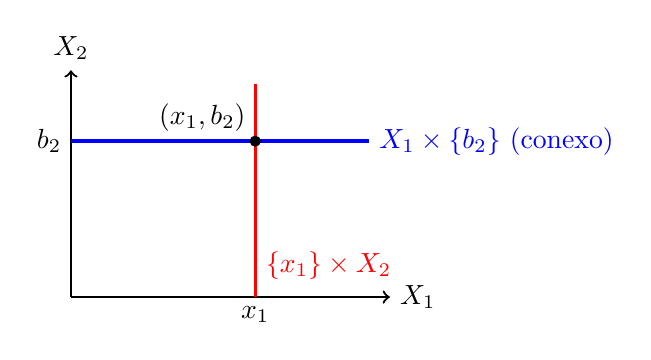
\begin{tikzpicture}[scale=0.9]
                % Ejes / Espacio producto X1 x X2
                \draw[->, thick] (0,0) -- (4.5,0) node[right] {$X_1$};
                \draw[->, thick] (0,0) -- (0,3.2) node[above] {$X_2$};
                
                % Línea horizontal X1 x {b2}
                \draw[very thick, blue] (0,2.2) -- (4.2,2.2) node[right] {$X_1 \times \{b_2\}$ (conexo)};
                \node[left] at (0,2.2) {$b_2$};
                
                % Línea vertical {x1} x X2
                \draw[very thick, red] (2.6,0) -- (2.6,3.0) node[right, pos=0.15] {$\{x_1\} \times X_2$};
                \node[below] at (2.6,0) {$x_1$};
                
                % Punto de intersección (x1, b2)
                \filldraw[black] (2.6,2.2) circle (2pt) node[above left] {$(x_1, b_2)$};
            \end{tikzpicture}
        \end{center}
        
        Observemos que la intersección de ambos subespacios es no vacía:
        \[
            (\{x_1\} \times X_2) \cap (X_1 \times \{b_2\}) = \{(x_1, b_2)\} \neq \emptyset \text{}
        \]
        Por tanto, la «cruz» $T_{x_1} = (\{x_1\} \times X_2) \cup (X_1 \times \{b_2\}) \subseteq X_1 \times X_2$ es conexa por ser unión de dos subespacios conexos con intersección no vacía.
        
        Consideremos ahora la unión de todas estas cruces al variar $x_1 \in X_1$:
        \[
            \bigcup_{x_1 \in X_1} T_{x_1} = X_1 \times X_2 \text{}
        \]
        (ya que cualquier par $(x_1, x_2) \in \{x_1\} \times X_2 \subseteq T_{x_1}$). Además, todas las familias $\{T_{x_1}\}_{x_1 \in X_1}$ comparten el segmento horizontal:
        \[
            \bigcap_{x_1 \in X_1} T_{x_1} = X_1 \times \{b_2\} \neq \emptyset \text{}
        \]
        En consecuencia, $X_1 \times X_2 = \bigcup_{x_1 \in X_1} T_{x_1}$ es conexo al ser unión de subespacios conexos con intersección total no vacía.

        \item \textbf{Paso inductivo ($n-1 \implies n$):} Supongamos como hipótesis de inducción que $\prod_{i=1}^{n-1} X_i$ es conexo. Como $\prod_{i=1}^n X_i$ es homeomorfo a $\left(\prod_{i=1}^{n-1} X_i\right) \times X_n$, aplicamos el caso $n = 2$ para concluir que $\prod_{i=1}^n X_i$ es conexo.
    \end{itemize}

    \paragraph{Caso 2: $I$ es un conjunto de índices cualquiera.}
    Fijemos un punto $b = (b_i)_{i \in I} \in \prod_{i \in I} X_i$. Para cada subconjunto finito $M = \{i_1, \dots, i_r\} \subseteq I$, definimos el subespacio:
    \[
        T_M = \left\{ (x_i)_{i \in I} \in \prod_{i \in I} X_i \;\middle|\; x_i = b_i \text{ si } i \notin M \right\} \text{}
    \]
    Observemos que $T_M$ es homeomorfo al producto finito $X_{i_1} \times \dots \times X_{i_r}$ (mediante la proyección sobre las coordenadas de $M$, ya que el resto están fijas en $b_i$). Por el \textbf{Caso 1}, $T_M$ es conexo para todo $M \subseteq I$ finito.

    Además, para todo $M \subseteq I$ finito se tiene que $b \in T_M$, luego:
    \[
        \bigcap_{\substack{M \subseteq I \\ M \text{ finito}}} T_M \ni b \implies \bigcap_{\substack{M \subseteq I \\ M \text{ finito}}} T_M \neq \emptyset \text{}
    \]
    Por tanto, el subespacio $Y = \bigcup_{\substack{M \subseteq I \\ M \text{ finito}}} T_M \subseteq \prod_{i \in I} X_i$ es conexo por ser unión de conexos con intersección no vacía.

    Probemos finalmente que $Y$ es denso en $\prod_{i \in I} X_i$ ($\overline{Y} = \prod_{i \in I} X_i$):
    \begin{quote}
        Sea $x = (x_i)_{i \in I} \in \prod_{i \in I} X_i$ y sea $U$ un abierto básico de la topología producto tal que $x \in U$. Por definición de la base producto, existe un subconjunto finito $M_U = \{i_1, \dots, i_m\} \subseteq I$ y abiertos $U_{i_j} \subseteq X_{i_j}$ tales que:
        \[
            \displaystyle U = U_{i_1} \times \dots \times U_{i_m} \times \prod_{i \notin M_U} X_i \text{}
        \]
        Definimos el punto $z = (z_i)_{i \in I} \in \prod_{i \in I} X_i$ mediante:
        \[
            z_i = \begin{cases} x_i & \text{si } i \in M_U, \\ b_i & \text{si } i \notin M_U. \end{cases} \text{}
        \]
        Por construcción, $z \in T_{M_U} \subseteq Y$. Por otro lado, para cada $j \in \{1, \dots, m\}$ se cumple $z_{i_j} = x_{i_j} \in U_{i_j}$, de modo que $z \in U$. Así, $z \in U \cap Y \neq \emptyset$ para todo abierto básico $U$ que contiene a $x$, lo que demuestra que $x \in \overline{Y}$.
    \end{quote}
    Como $Y$ es conexo y $\overline{Y} = \prod_{i \in I} X_i$, concluimos que $\prod_{i \in I} X_i$ es conexo (pues el cierre de un subespacio conexo es conexo).
\end{dem}


%====================================================
%17/11/2026
%====================================================

\section{Componentes conexas}

Sea $X$ espacio topol\'ogico
\begin{defi}
    Sea $R$ la relaci\'on de equivalencia dada por 
    \begin{center}
        $xRy$ si existe un subespacio conexo $A\subset X$ tal que $x,y\in A$ 
    \end{center}
\end{defi}
\begin{prop}
    Efectivamente, es relaci\'on de equivalencia.
\end{prop}
\begin{dem}
    Reflexiva: $xRx$ pues $x\in \{x\}$ y es conexo.
    
    Sim\'etrica: Si $xRy \Rightarrow yRx$, si $x,y\in A$, $x, y\in A$

    Transitiva: Si $xRy$ e $yRz \Rightarrow xRz$. Ambas implican que $x,y \in A$ conexo, $y,z \in B$ conexo, luego $x,z\in A\cup B$ y es conexo pues $y\in A\cap B \neq \emptyset$. 
\end{dem}
\begin{defi}
    Las \textbf{componentes conexas} de $X$ son las clases de equivalencia de la relaci\'on $R$ anterior. 
\end{defi}
\begin{obs}
    Como las clases de equivalencia son disjuntas, las componentes conexas son disjuntas dos a dos. Adem\'as, su uni\'on es $X$ (pues todo elemento est\'a en alguna clase).
    
    Es decir, si $\{C_i\}_{i \in I}$ son las componentes conexas $\Rightarrow X = \coprod_{i \in I} C_i$. 
    
   \textit{Observaci\'on importante:} esta uni\'on es de conjuntos, NO de espacios topol\'ogicos. Esto es porque $C_j \hookrightarrow \coprod C_i$ es abierto-cerrado, pero $C_j \hookrightarrow X$ es cerrado, no podemos asegurar que sea abierto (lo veremos m\'as adelante). Si $I$ es finito s\'i es igualdad de espacios topol\'ogicos.
\end{obs}
\begin{prop}
Las componentes conexas son los mayores subespacios conexos de $X$. Es decir, si $C$ conexo y si $C \subset A$ con $A$ conexo, entonces $C=A$.
\end{prop}
\begin{dem}
    Sea $C$ componente conexa de $X\Rightarrow C=[x]=C_x$ con $x\in X$. Si $C \subset A$ conexo, se verifica que para todo $y\in A$, $x,y\in A \Rightarrow xRy \Rightarrow y\in [x] = C \Rightarrow C=A$. Falta demostrar que $C$ es conexo (suponer que no lo es, separarlo, habr\'a puntos relacionados en cada separaci\'on pero tienen que estar en el mismo conexo...). 
\end{dem}
\begin{cor}
    Las componentes conexas son cerradas
\end{cor}
\begin{dem}
    Sea $C$ componente conexa $\Rightarrow C$ es conexo $\Rightarrow \overline{C}$ es conexo y $C \subset \overline{C}$ luego tenemos un conexo que contiene a $C$ y por la proposici\'on anterior, $C = \overline{C}$. 
\end{dem}
\begin{custom}
[Proposici\'on] Para cada $x\in X$ existe una \'unica componente conexa de $X$ que contiene a $x$, y la denotamos por $C_x$. Por ser $x\in[x] = C_x$ disjuntas.

Si $y \in C_x = [x] \Rightarrow C_x=C_y$ por $C_y=[y]=[x]=C_x$. 

Si $A\subset X$ es un subespacio conexo de $X$, entonces $A$ est\'a contenido en una \'unica componente conexa. 

$\forall\, x,y\in A \Rightarrow xRy \Rightarrow[x] = [y] = C_x \supset A$.
\end{custom}

Para estudiar $f:X \longrightarrow Y$ se puede reducir a ver sus componentes conexas
$$\bt \coprod C_i = X \rar{f} & Y \\[5mm] \arrow[hook]{u} C_i \arrow[swap]{ru}{f|_{C_i}} \et$$
entonces si $X$ no es conexo se separa en sus componentes, y as\'i se puede suponer siempre que $X$ es conexo. 
\begin{defi}
    Un espacio topol\'ogico $X$ es totalmente inconexo o disconexo si sus componentes conexas son los puntos. 
\end{defi}

Si $X$ es conexo, su \'unica componente conexa es $C_x= X \quad \forall \, x\in X$. Es decir, si $X$ es conexo las componentes conexas no aportan nada.

\begin{ejems}
\begin{enumerate}
    \item $(X, \mc T_{dis})$ es totalmente inconexo, pues si $y,y' \in Y\subset X$, entonces $Y = \{y\} \cup (Y-\{y\})$ es una separaci\'on no trivial luego $Y$ no es conexo. Como es general, los mayores subespacios conexos son los puntos, y as\'i el espacio es totalmente inconexo. 
    \item $(X, \mc T_A)$. $U$ es abierto si y solo si $A \subset U$ \'o $U=\emptyset$. Sea $Y \subset X$, 
    \begin{enumerate}
        \item $Y \cap A = \emptyset \iff Y$ es cerrado.
        
        Supongamos $Y$ conexo. Sean $y\neq y' \in Y$, $Y = \{y\} \cup (Y-\{y\})$ es cerrado en $X$ (luego en $Y$) $\cup$ cerrado en $X$ (luego en $Y$), y entonces tenemos una separaci\'on no trivial en $Y$, contradiciendo que $Y$ es conexo, al suponer que $y\neq y'$ luego $Y=\{y\}$. Los \'unicos conexos que no cortan a $A$ son los puntos.
        \item Si $Y\cap A \neq \emptyset$
        
        Sea $y\in Y\cap A$. Sean $V_1,V_2$ separaci\'on de $Y$, entonces existe $(U_1,U_2)$ abiertos de $X$ con $U_i \cap Y = V_i$, y por ser abiertos, 
        $$\begin{cases} A\subset U_1 \\[-3mm] \text{y} \\[-3mm] A\subset U_2  \end{cases} 
        \Rightarrow 
        \begin{cases}
            A\cap Y \subset U_1 \cap Y=V_1 \\[-3mm] \text{y} \\[-3mm] A\cap Y \subset U_2 \cap Y = V_2
        \end{cases}$$ de forma que $A\cap Y\subset V_1 \cap V_2$,  llegando a contradicci\'on con que $V_1$ y $V_2$ es separci\'on. Esto implica que $Y$ es conexo. 

        Adem\'as $X$ es conexo porque $A\subset X \equiv A\cap X \neq \emptyset$. 
    \end{enumerate}
\begin{ejer}
    $(X, \mc T^A)$ es igual que la de $\mc T_A$, basta estudiarlo por cerrados.  
\end{ejer}

    \item $(X, \mc T_{\mathrm{dis}})$ totalmente inconexo.
    \item $(X, \mc T_A)$ \qquad $(X, \mc T^A)$.
    \item $(X, \mc T_{\mathrm{cof}})$, $Y \subset X$:
    \begin{itemize}
        \item \textbf{$Y$ finito:} $Y = \{y_1, \dots, y_r\} = \{y_1\} \cup \{y_2, \dots, y_r\}$ (separación no trivial). Si $r > 1$, $Y$ es conexo si $Y$ tiene un solo punto.
        \item \textbf{$Y$ infinito:} $Y = \overbrace{(C_1 \cap Y)}^{\text{finito}} \cup \overbrace{(C_2 \cap Y)}^{\text{finito}}$, donde $C_i \subset X$ son cerrados finitos. Si formara una separación, $\Rightarrow$ $Y$ no admite separación no trivial $\Rightarrow$ $Y$ conexo.
    \end{itemize}

\paragraph{¿$(X, \mc T_{\mathrm{cof}})$ es conexo?}
\begin{itemize}
    \item Si $X$ es finito, es totalmente inconexo.
    \item Si $X$ es infinito $\Rightarrow$ $X$ es conexo.
\end{itemize}
    \item $(\mathbb{R}, \mc T_{\mathrm{kol}})$, donde $\mc T_{\mathrm{kol}} = \{(a, \infty) \mid a \in \mathbb{R}\} \cup \{\emptyset, \mathbb{R}\}$.

    Sean $U, V \subset \mathbb{R}$ abiertos; entonces $U \cap V \in \{U, V\}$ (si son no vacíos y están anidados).

    Si $Y \subset \mathbb{R}$ (no vacío) admite una descomposición $Y = (U \cap Y) \cup (V \cap Y)$ con $\emptyset = (U \cap Y) \cap (V \cap Y) = (U \cap V) \cap Y$, como $U \cap V$ es uno de ellos:
    \[
        \Rightarrow \begin{cases} U = \emptyset \text{ y } V \text{ total} \\ V = \emptyset \text{ y } U \text{ total} \end{cases}
        \Rightarrow Y \text{ no admite separaciones no triviales} \Rightarrow Y \text{ conexo.}
    \]
    (\emph{«Cualquier subespacio de $(\mathbb{R}, \mc T_{\mathrm{kol}})$ es conexo»}.)
    \item $(\mathbb{R}, \mc T_{\mathrm{sorg}})$, donde $\mc T_{\mathrm{sorg}} = \langle [a,b) \rangle$. Los conjuntos $(-\infty, a)$ y $[a, +\infty) = \bigcup_{b > a} [a,b)$ son abiertos en $\mc T_{\mathrm{sorg}}$.
    \[
        \mathbb{R} = (-\infty, a) \cup [a, +\infty) \implies \mathbb{R} \text{ no es conexo con } \mc T_{\mathrm{sorg}}.
    \]
    Dado $Y \subset \mathbb{R}$ con $a \in Y$, se tiene $Y \subset [a, +\infty)$. Si $Y$ posee otro punto $a' \in Y$ distinto de $a$, con $a < a'$, entonces:
    \[
        Y = \big([a, a') \cap Y\big) \cup \big([a', +\infty) \cap Y\big)
    \]
    es una separación no trivial (con $a \in [a, a') \cap Y$ y $a' \in [a', +\infty) \cap Y$ abiertos relativos no vacíos), luego $Y$ no es conexo. Por tanto, los únicos subconjuntos conexos son los puntos (y el vacío), y $(\mathbb{R}, \mc T_{\mathrm{sorg}})$ es totalmente inconexo.

    \item $(\mathbb{R}, \mc T_d) \supset \mathbb{Q}$. ¿Es $\mathbb{Q}$ conexo?
    Para cualquier irracional $\alpha \in \mathbb{I}$ ($\alpha \notin \mathbb{Q}$):
    \[
        \mathbb{Q} = \big((-\infty, \alpha) \cap \mathbb{Q}\big) \cup \big((\alpha, +\infty) \cap \mathbb{Q}\big)
    \]
    es una separación no trivial, luego $\mathbb{Q}$ no es conexo. Además, para cualquier $Y \subset \mathbb{Q}$ con $y, y' \in Y$ y $y < y'$, existe $\alpha \in \mathbb{I}$ tal que $y < \alpha < y'$, y
    \[
        Y = \big((-\infty, \alpha) \cap Y\big) \cup \big((\alpha, +\infty) \cap Y\big)
    \]
    es una separación no trivial (con $y$ en el primer conjunto y $y'$ en el segundo), luego $Y$ no es conexo. En consecuencia, $\mathbb{Q}$ es totalmente inconexo.
\end{enumerate}
\end{ejems}
\begin{cor}[de los resultados previos de conexos]
Si $f \colon X \to Y$ es continua y $X$ es conexo, entonces la gráfica de $f$, $\Gamma_f \subset X \times Y$, es un subespacio conexo.
\end{cor}

\begin{dem}
Consideramos la aplicación $\gamma_f \colon X \to X \times Y$ definida por $\gamma_f(x) = (x, f(x))$, cuya imagen es $\operatorname{Im} \gamma_f = \Gamma_f$ (notación: $\gamma_f \leftrightarrow \Gamma_f = (1 \times f)$). Esta aplicación es continua pues al componer con las dos proyecciones es continua (propiedad universal de la topología inicial). Como $X$ es conexo, su imagen continua $(1 \times f)(X) = \Gamma_f$ es conexa.
\end{dem}

\section{Espacios arcoconexos o conexos por caminos}

Sea $X$ un espacio topológico y $x, x' \in X$.

\begin{defi}
Un \textbf{camino} en $X$ que une $x$ con $x'$ es una aplicación continua $f \colon [0,1] \to X$ (o sobre cualquier intervalo $[a,b]$) con $f(0) = x$ y $f(1) = x'$. $\operatorname{Im} f \subset X$ es la traza/imagen del camino (i.e., el camino es la aplicación o su imagen).
\end{defi}

\begin{defi}
Dado un camino $f \colon [0,1] \to X$, se define el \textbf{camino opuesto} $(-f) \colon [0,1] \to X$ por $(-f)(t) = f(1-t)$ («recorrer el camino en sentido contrario»).
\end{defi}

\begin{propi}
Si tenemos dos caminos $f$ (que une $x$ con $x'$) y $g$ (que une $x'$ con $x''$), entonces existe el \textbf{camino unión o camino suma} $(f \cup g) \colon [0,2] \to X$ (por comodidad, o reparametrizado en $[0,1]$) definido por:
\[
(f \cup g)(t) = \begin{cases}
f(t) & \text{si } 0 \le t \le 1, \\
g(t-1) & \text{si } 1 \le t \le 2.
\end{cases}
\]
Se cumple $(f \cup g)(0) = f(0) = x$ y $(f \cup g)(2) = g(1) = x''$, por lo que $(f \cup g)$ une $x$ con $x''$. Además, $f \cup g$ es continua pues $f(1) = g(0)$ (el único punto crítico es $t = 1$).
\end{propi}
\begin{defi}
Un \textbf{lazo} en el punto $x$ es un camino con origen y final en el punto $x$, es decir, $f(0) = f(1) = x$.

\begin{center}
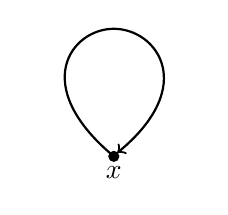
\begin{tikzpicture}[scale=0.9]
    \draw[thick, ->] (0,0) .. controls (-1.2, 1.0) and (-0.6, 1.8) .. (0, 1.8)
        .. controls (0.6, 1.8) and (1.2, 1.0) .. (0.05, 0.05);
    \filldraw[black] (0,0) circle (2pt) node[below] {$x$};
\end{tikzpicture}
\end{center}
\end{defi}

\begin{ejem}
En $\mathbb{R}^2 \setminus \{(0,0)\}$, un lazo rodeando el origen no se puede encoger «tirando» de él sin salir del espacio (no da tiempo a ver homotopías ni grupo fundamental).

\begin{center}
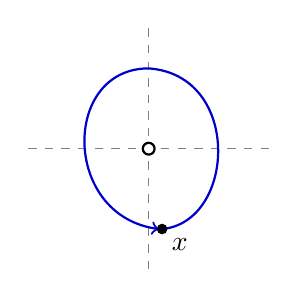
\begin{tikzpicture}[scale=0.85]
    % Ejes punteados
    \draw[dashed, gray] (-1.8,0) -- (1.8,0);
    \draw[dashed, gray] (0,-1.8) -- (0,1.8);
    % Agujero en el origen
    \draw[thick, fill=white] (0,0) circle (2.5pt);
    % Lazo alrededor del origen
    \draw[thick, blue!80!black, ->] (0.2, -1.2) .. controls (1.3, -1.1) and (1.4, 1.1) .. (0, 1.2)
        .. controls (-1.3, 1.2) and (-1.3, -1.0) .. (0.15, -1.2);
    \filldraw[black] (0.2, -1.2) circle (2pt) node[below right] {$x$};
\end{tikzpicture}
\end{center}
\end{ejem}

\begin{defi}
Un espacio topológico $X$ es \textbf{arcoconexo} (o conexo por caminos) si para cualesquiera dos puntos $x, x' \in X$ existe un camino en $X$ que los une.
\end{defi}

\begin{ejems} \,
\begin{itemize}
    \item \textbf{$(\mathbb{R}^2, \mc T_d)$ es arcoconexo:} dados $x, x' \in \mathbb{R}^2$, el segmento $f(t) = x + t(x' - x)$ ($t \in [0,1]$) es un camino continuo que une $x$ con $x'$.

    \begin{center}
    \begin{tikzpicture}[scale=0.85]
        \draw[thick, blue!80!black] (0,0) .. controls (1.2, 0.4) and (2.2, 0.8) .. (3.2, 1.3);
        \filldraw[black] (0,0) circle (2pt) node[below left] {$x$};
        \filldraw[black] (3.2,1.3) circle (2pt) node[above right] {$x'$};
    \end{tikzpicture}
    \end{center}

    \item \textbf{$\mathbb{R}^2 \setminus \text{eje } x$ (con la usual) no es arcoconexo:} no todo par de puntos se puede unir con un camino (por ejemplo, un punto en el semiplano superior y otro en el semiplano inferior no pueden conectarse sin cruzar el eje $x$).

    \begin{center}
    \begin{tikzpicture}[scale=0.85]
        \draw[dashed, gray] (-1.8,0) -- (1.8,0) node[right, black, font=\footnotesize] {eje $x$};
        \draw[thick] (0,-1.8) -- (0,1.8);
        \filldraw[blue!80!black] (0.5, 0.9) circle (2pt);
        \filldraw[blue!80!black] (0.5, -0.9) circle (2pt);
    \end{tikzpicture}
    \end{center}

    \item \textbf{Las bolas $B_d(x, \varepsilon) \subset \mathbb{R}^2$ (con la usual) son arcoconexas:} por convexidad/estrellamiento, cualesquiera dos puntos $x', x''$ de la bola se unen mediante el segmento en su interior.

    \begin{center}
    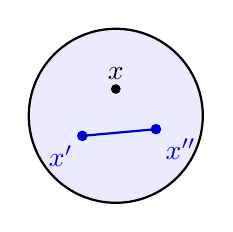
\begin{tikzpicture}[scale=0.85]
        \draw[thick, fill=blue!8] (0,0) circle (1.3cm);
        \filldraw[black] (0, 0.4) circle (1.8pt) node[above] {$x$};
        \filldraw[blue!80!black] (-0.5, -0.3) circle (2pt) node[below left] {$x'$};
        \filldraw[blue!80!black] (0.6, -0.2) circle (2pt) node[below right] {$x''$};
        \draw[thick, blue!80!black] (-0.5, -0.3) -- (0.6, -0.2);
    \end{tikzpicture}
    \end{center}
\end{itemize}
\end{ejems} \cleardoublepage

\chapter{Espacios compactos}
\section{Subespacios compactos y propiedades fundamentales}
Sea $X$ un espacio topol\'ogico
\begin{defi}
    Un \textbf{recubrimiento} de $X$ es una familia de abiertos $\{U_i\}_{i \in I}$ tal que $\displaystyle X = \bigcup_{i \in I} U_i$. 
\end{defi}
\begin{defi}
    Un espacio topol\'ogico $X$ es \textbf{compacto} si \underline{para todo} recubrimiento $\{U_i\}_{i \in I}$ existe un subrrecubrimiento finito, es decir, existen $i_1, \ldots, i_r \in I$ tal que $\{U_{i_1}, \ldots, U_{i_r}\}$ recubren $X$
\end{defi}
\begin{ejem}
$\bb R$ no es compacto. $\{U_n = (-n,n): n \in \bb N\}$ recubrimiento de $\bb R$. Si existen $n_1, \ldots, n_r \in \bb N$ tal que 
$$\bigcup_{j=1}^r U_{n_j} = (-n_1, n_1)\cup \cdots \cup (-n_r,n_r) = (-n,n) \neq \bb R$$
con $n = \max\{n_{i_j}\}$ entonces no recubren.

Otro ejemplo es el recubrimiento $\left\{V_n = \left(n- \frac{1}{|n|}, (n+1) + \frac{1}{|n|} \right)\right\}_{n\in \bb Z}$.
\end{ejem}
\begin{defi}
    Un \textbf{subespacio} topol\'ogico $Y \subset X$ es \textbf{compacto} si lo es como espacio topol\'ogico, es decir, si $(Y, \mc T_X|_Y)$ es compacto.
\end{defi}
\begin{prop}
$Y \subset X$ es subespacio compacto $\iff$ para toda familia de abiertos $\{U_i\}_{i \in I}$ de $X$ tal que $Y \subset \bigcup_{i \in I} U_i$ existen $\{i_1, \ldots, i_r\}\subset I$ tal que $Y \subset U_{i_r} \cup \cdots U_{i_r}$.
\end{prop}
\begin{dem} \,
\begin{itemize}
    \item[$\Rightarrow)$] $Y\subset \displaystyle \bigcup_{i \in I} U_i$, entonces $Y= \displaystyle \bigcup_{i \in I} (U_i\cap Y)$ y $ U_i\cap Y \in \mc T_X|_Y$, luego por ser $Y$ compacto, y tener un subrrecubrimiento finito, entonces
    $$Y = \bigcup_{j=1}^r U_{i_j} \cap Y \subset \bigcup_{j=1}^r U_{i_j}$$
    Por tanto, $\{U_{i_1}, \ldots, U_{i_r}\}$ recubre a $Y$.
    \item[$\Leftarrow)$] Sea $\{ V_i \}_{i\in I}$ recubrimiento de $Y$ por abiertos de $Y$, entonces existen $\{U_i\}_{i\in I}$ abiertos de $X$ tal que $U_i \cap Y = V_i\, \forall i \in I$. 
    $$Y = \bigcup_{i\in I} V_i = \bigcup_{i\in I} (U_i \cap Y) \subset \bigcup_{i\in I} U_i$$
    por lo que existen $i_1, \ldots, i_r \in I$ tales que $Y \subset (U_{i_1} \cup \cdots \cup U_{i_r})$, luego
    $$Y = Y \cap Y \subset (U_{i_1} \cup \cdots \cup U_{i_r}) \cap Y = \underbrace{(U_{i_1}\cap Y)}_{V_{i_1}} \cup \cdots \cup \underbrace{(U_{i_r}\cap Y)}_{V_{i_r}}$$
    por lo que $Y = V_{i_1} \cup \cdots \cup V_{i_r}$, lo que demuestra que $\{V_{i_1}, \ldots, V_{i_r}\}$ es un subrrecubrimiento finito de $Y$, por lo que $(Y,\mc T_X|_Y)$ es compacto. 
\end{itemize}
\end{dem}
\begin{prop}[Todo cerrado de un compacto es compacto]
Si $X$ es compacto y $Y \subset X$ es cerrado $\Rightarrow$ $Y$ es compacto. 
\end{prop}
\begin{dem}
Sean $\{U_i\}_{i\in I}$ abiertos de $X$ con $\displaystyle Y \subset \bigcup_{i\in I} U_i$, como $Y$ es cerrado, $X-Y$ es abierto, de forma que 
$$X = Y \cup (X-Y) \subset \bigcup_{i\in I} U_i \cup (X-Y) \subset X \Rightarrow X = \bigcup_{i\in I} U_i \cup (X-Y)$$
es un recubrimiento de $X$ por abiertos de $X$, pero por ser $X$ compacto, existe $\{i_1, \ldots, i_r \} \subset I$ tal que $X = U_{i_1} \cup \cdots \cup U_{i_r} \cup (X-Y)$ (puede que $X-Y$ aparezca o no en él; en cualquier caso, al añadirlo se mantiene la igualdad). Finalmente, dado cualquier $y \in Y$, se tiene $y \in X$ e $y \nin X-Y$, por lo que necesariamente $y \in U_{i_1} \cup \cdots \cup U_{i_r}$. Por tanto $Y \subset U_{i_1} \cup \cdots \cup U_{i_r}$ y se concluye que $Y$ es compacto. 
\end{dem}
\section{Compacidad y espacios de Hausdorff ($T_2$)}
\begin{prop}
Sea $X$ espacio topol\'ogico $T_2$ e $Y\subset X$ subespacio compacto. Entoces se verifica que para todo $x\nin Y$ existen abiertos $U_x, U_Y$ de $X$ tal que 
$$x\in U_x, \quad Y \subset U_Y \quad \text{con} \quad U_x\cap U_Y =\emptyset$$
\end{prop}
\begin{obs}
    Esta propiedad es análoga a la definición de espacio regular, pero separando un punto de un compacto en lugar de un cerrado arbitrario.
\end{obs}
\begin{dem}
Sea $x\nin Y$, dado $y\in Y$, claramente $x\neq y$ por ser $X$ separado, entonces existen abiertos 
$$x\in U_x^y, \quad y \in U_y \quad \text{con} \quad U_x^y \cap U_y =\emptyset$$
(nótese que el abierto $U_x^y$ depende tanto del punto $x$ como del punto $y\in Y$ considerado). Al variar $y$ en todo $Y$, la familia $\{U_y\}_{y \in Y}$ es una familia de abiertos de $X$ que recubre a $Y$, puesto que cada $y \in Y$ pertenece a su correspondiente $U_y$: 
$$Y\subset \bigcup_{y\in Y} U_y$$
y como $Y$ es compacto, entonces existen $y_1, \ldots, y_r \in Y$ tales que 
$$Y \subset U_{y_1}\cup \cdots \cup U_{y_r} \eqqcolon U_Y$$
Definimos
$U_x \coloneqq U_x^{y_1} \cap \cdots \cap U_x^{y_r}$ que es abierto por ser intersecci\'on finita. 
Comprobamos que cumplen todas las condiciones exigidas:
\begin{itemize}
    \item \textbf{Son abiertos de $X$:} $U_Y$ es abierto por ser unión de abiertos, y $U_x$ es abierto por ser \textbf{intersección finita} de abiertos.
    \item \textbf{Contienen a $x$ y a $Y$:} Por construcción, $Y \subseteq U_Y$. Además, como $x \in U_x^{y_j}$ para todo $j \in \{1, \dots, r\}$, se tiene $x \in \displaystyle \bigcap_{j=1}^r U_x^{y_j} = U_x$.
    \item \textbf{Son disjuntos:} $U_x\cap U_Y = \emptyset$. Sea $z\in U_x \cap U_Y$
    $$\Rightarrow \begin{cases}
        z\in U_x \Rightarrow z \in U_x^{y_j} \forall j=1,\ldots, r \\ z\in U_Y \Rightarrow z \in U_{y_{j_o}} \text{ para alg\'un } j_o \in \{1, \ldots, r\}
    \end{cases}$$
    luego $z\in U_x^{y_{j_o}}\cap U_{y_{j_o}} = \emptyset$, lo cual es una contradicci\'on al suponer que $z \in U_x \cap U_y$. 
\end{itemize}
\end{dem}
\begin{cor}[Todo compacto en un espacio $T_2$ es cerrado]
Si $X$ es $T_2$ e $Y\subset X$ es compacto $\Rightarrow Y$ es cerrado. En particular, si $X$ es $T_2$ y compacto, un subespacio $Y\subset X$ es compacto $\iff$ $Y$ es cerrado. 
\end{cor}
\begin{dem}
    $Y$ cerrado $\iff \, X-Y$ es abierto $\iff$ $\forall x\in X-Y$ existe un abierto $U_x$ con $x\in U_x \subset X-Y$ (entorno de todos sus puntos). 
    
    Sea $x\nin Y$, por hip\'otesis $Y$ es compacto, luego existen abiertos $U_x, UYy$ tales que $x\in U_x, Y \subset U_Y$ con $U_x\cap U_Y =\emptyset$ luego
    $$U_x\cap Y \subset U_x\cap U_Y = \emptyset \Rightarrow U_x\cap Y = \emptyset \Rightarrow U_x \subset X-Y$$ Así, todo punto $x \in X - Y$ posee un entorno abierto $U_x$ contenido en $X - Y$ (es decir, $X - Y = \bigcup_{x \in X - Y} U_x$), de modo que $X - Y$ es abierto y, por tanto, $Y$ es cerrado en $X$.

    Para la segunda afirmación, supongamos que $X$ es $T_2$ y compacto:
    \begin{itemize}
        \item[$\Rightarrow)$] Si $Y \subseteq X$ es compacto, entonces $Y$ es cerrado por lo que acabamos de demostrar (usando que $X$ es $T_2$).
        \item[$\Leftarrow)$] Si $Y \subseteq X$ es cerrado, entonces $Y$ es compacto por la Proposición 2 (usando que $X$ es compacto). \qedhere
    \end{itemize}
\end{dem}
\section{Aplicaciones continuas}
\begin{prop}[La imagen continua de un compacto es compacta]
    Si $f: X \longrightarrow Y$ es continua y $X$ es compacto entonces $f(X) = \Im \, f$ es compacto. 
\end{prop}
\begin{dem}
Veamos que $f(X)$ es un subespacio compacto de $Y$. Sea $\{V_i\}_{i \in I}$ una familia de abiertos de $Y$ tal que
\[
    f(X) \subseteq \bigcup_{i \in I} V_i.
\]
Tomando antiimágenes por $f$ y usando sus propiedades elementales
\[
    X = f^{-1}(f(X)) \subseteq f^{-1}\!\left(\bigcup_{i \in I} V_i\right) = \bigcup_{i \in I} f^{-1}(V_i) \subseteq X,
\]
y como $f^{-1}(V_i)\subset X$, resulta la igualdad $\displaystyle X = \bigcup_{i \in I} f^{-1}(V_i)$.

Como $f$ es \textbf{continua} y cada $V_i$ es abierto en $Y$, cada conjunto $f^{-1}(V_i)$ es abierto en $X$. Por tanto, $\{f^{-1}(V_i)\}_{i \in I}$ es un recubrimiento abierto de $X$.

Dado que $X$ es compacto, existen índices $\{i_1, \dots, i_r\} \subset I$ tales que:
\[
    X = f^{-1}(V_{i_1}) \cup \dots \cup f^{-1}(V_{i_r}) = \bigcup_{j=1}^r f^{-1}(V_{i_j}).
\]
Aplicando ahora $f$ a ambos miembros y recordando que $f(f^{-1}(B)) \subseteq B$ para todo subconjunto $B \subseteq Y$:
\[
    f(X) = f\!\left(\bigcup_{j=1}^r f^{-1}(V_{i_j})\right) = f\!\left(f^{-1}\!\left(\bigcup_{j=1}^r V_{i_j}\right)\right) \subseteq \bigcup_{j=1}^r V_{i_j}.
\]
Hemos encontrado así una subfamilia finita $\{V_{i_1}, \dots, V_{i_r}\}$ que recubre a $f(X)$, por lo que $f(X)$ es compacto.
\end{dem}
\begin{ejer}
$\bb R^n$ no es compacto $\forall n$. 
\end{ejer}\begin{dem}
Consideramos la proyecci\'on can\'onica $\pi_1: \bb R^n \longrightarrow \bb R$ que es continua (por la definici\'on de la topolog\'ia producto $\mc T_{\pi} = \mc T_d$ usual) y epiyectiva, luego $\pi_1(\bb R^n) = \bb R$.

Por la proposici\'on anterior la imagen continua de un compacto es compacta. Si $\bb R^n$ fuera compacto, su imagen por $\pi_1$, $\pi_1(\bb R^n) = \bb R$ debe ser compacto, pero sabemos que $\bb R$ no es compacto. Por tanto $\bb R^n$ no es compacto.  
\end{dem}
\cleardoublepage


% APÉNDICES ----------------------------------------------------------
\appendix %estilo apéndices

%
\includepdf[pages=2-15]{Appendixes/ejers1-4.pdf}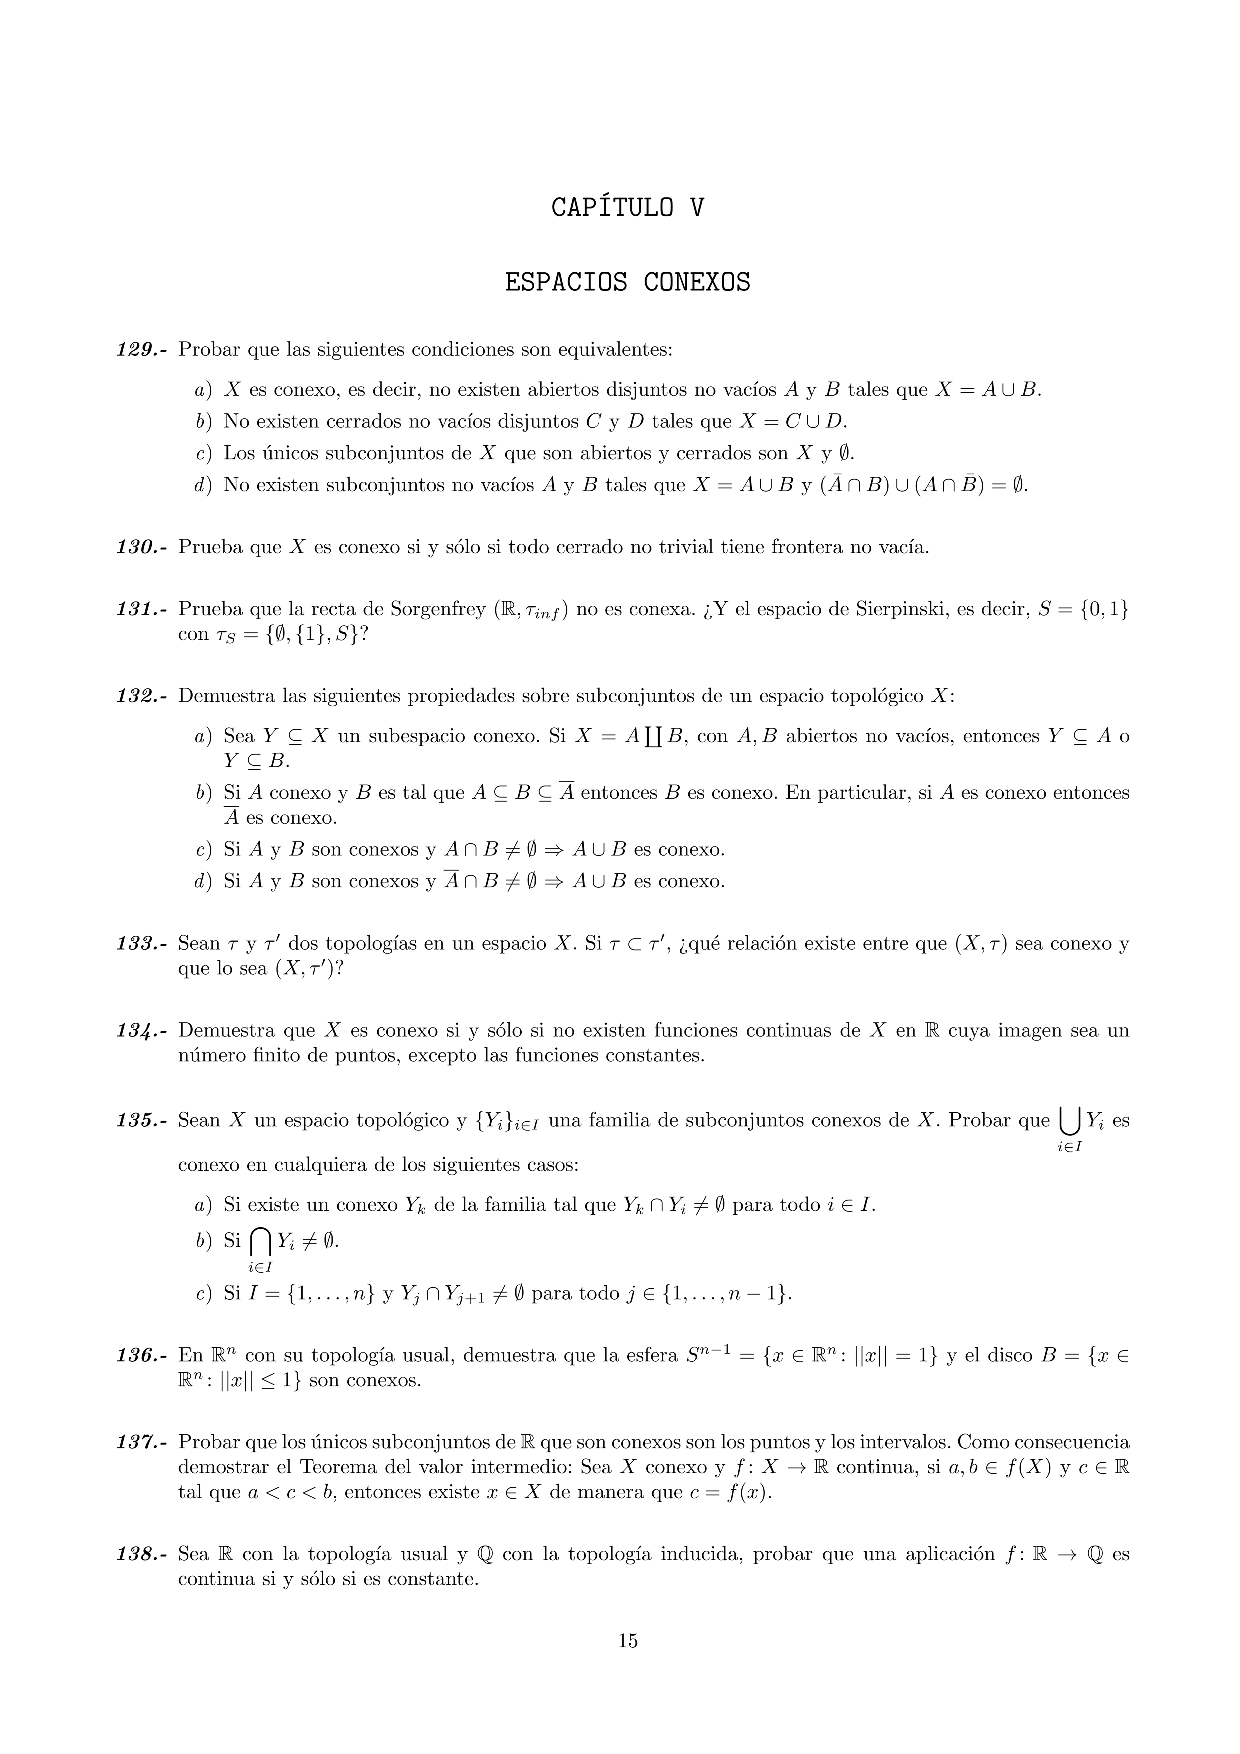
\includepdf[pages=1-3]{Appendixes/Problemas.Tema 5.pdf} 
\chapter{Enunciados ejercicios}
\section*{Capítulo I. Espacios topológicos}

\begin{ejer}[1]
Dado $X = \{a,b,c,d,e\}$ se consideran las siguientes familias de subconjuntos de $X$:
\begin{align*}
    \mathcal{T}_1 &= \{X, \emptyset, \{a\}, \{c,d\}, \{a,c,d\}, \{a,b,c,d\}\}, \\
    \mathcal{T}_2 &= \{X, \emptyset, \{a\}, \{d,e\}, \{a,c,d\}, \{b,c,d,e\}\}, \\
    \mathcal{T}_3 &= \{X, \emptyset, \{a\}, \{c,d\}, \{a,c,d\}, \{b,c,d\}\}.
\end{align*}
Determina cuáles de las $\mathcal{T}_i$ forman una topología por abiertos del conjunto $X$. Determinar los cerrados para las $\mathcal{T}_i$ que sean topologías.
\end{ejer}

\begin{ejer}[2]
Sea $X$ un conjunto y $A$ y $B$ subconjuntos no triviales. Determina bajo qué condiciones las familias
\[
    \mathcal{T}_1 = \{\emptyset, A, X\} \qquad \text{y} \qquad \mathcal{T}_2 = \{\emptyset, A, B, X\}
\]
forman una topología.
\end{ejer}

\begin{ejer}[3]
Demuestra que $\mathcal{T} = \{\emptyset, \mathbb{N}\} \cup \{A \subset \mathbb{N} \mid A \text{ contenga tan sólo números pares}\}$ determina una topología de $\mathbb{N}$. Determina si los siguientes subconjuntos son abiertos, cerrados, las dos cosas o ninguna de las dos:
\[
    A_1 = \{90, 2^{10}, 5^{21}-1\}, \qquad A_2 = \{\text{números primos}\} \qquad \text{y} \qquad A_3 = \{\text{números impares}\}.
\]
\end{ejer}

\begin{ejer}[4]
Sea $\mathcal{T}$ la familia de subconjuntos de $\mathbb{N}$ dada por $\mathbb{N}$, $\emptyset$ y los subconjuntos de la forma $E_n = \{n, n+1, n+2, \dots\}$. Probar que esta familia es una topología de $\mathbb{N}$.
\end{ejer}

\begin{ejer}[5]
En $\mathbb{Z}_+$ consideramos la familia de subconjuntos $U \subseteq \mathbb{Z}_+$ que satisfacen la siguiente propiedad: si $n \in U$, entonces cada divisor de $n$ también pertenece a $U$. Probar que dicha familia de subconjuntos es una topología en $\mathbb{Z}_+$, que no es la discreta.
\end{ejer}

\begin{ejer}[6]
\textbf{Topología del punto incluido.} Sea $X$ un conjunto y $a \in X$ un punto. Estudia si la familia de subconjuntos $\mathcal{T}_a$ formada por el vacío y los subconjuntos $U \subseteq X$ tales que $a \in U$ define una topología por abiertos de $X$.
\end{ejer}

\begin{ejer}[7]
\textbf{Topología del punto excluido.} Sea $X$ un conjunto y $a \in X$ un punto. Estudia si la familia de subconjuntos $\mathcal{T}_{a^c}$ formada por $X$ y los subconjuntos $U \subseteq X$ tales que $a \notin U$ define una topología por abiertos de $X$.
\end{ejer}

\begin{ejer}[8]
Sea $X$ el intervalo cerrado $[-1,1]$ de $\mathbb{R}$ y $\mathcal{T} = \{U \subset X : 0 \notin U\} \cup \{U \subseteq X : (-1,1) \subseteq U\}$. Probar que $(X, \mathcal{T})$ es un espacio topológico.
\end{ejer}

\begin{ejer}[9]
Sea $\mathcal{T}$ la familia de subconjuntos de $\mathbb{R}$ consistente en $\mathbb{R}$, $\emptyset$ y los intervalos abiertos no acotados $A_q = (q, \infty)$ donde $q \in \mathbb{Q}$. Demuestra que $\mathcal{T}$ no es una topología por abiertos de $\mathbb{R}$.
\end{ejer}

\begin{ejer}[10]
Sea $(X, \mathcal{T})$ un espacio topológico. Entonces $\mathcal{T}$ es la topología discreta si y sólo si para cada $x \in X$ el subconjunto que define $\{x\}$ es abierto.
\end{ejer}

\begin{ejer}[11]
Demuestra que la familia de subconjuntos de $\mathbb{R}$ dada por $\mathcal{T} = \{(-n, n) \mid n \in \mathbb{N}\} \cup \{\emptyset, \mathbb{R}\}$ define una topología por abiertos. ¿Cuál es el mayor abierto contenido en $[-2, 3)$? ¿Quiénes son los cerrados? ¿Cuál es el mínimo cerrado que contiene a los subconjuntos $(0,1)$, $\{3\}$, $\{1,4\}$ y $[-2,3)$?
\end{ejer}

\begin{ejer}[12]
Repetir el ejercicio 11 para las familias:
\begin{enumerate}
    \item[a)] $B = \{\emptyset, \mathbb{R}, (0, \infty), (0, n) \text{ con } n \in \mathbb{N}\}$.
    \item[b)] $C = \{\emptyset, \mathbb{R}, [-n, n] \text{ con } n \in \mathbb{N}\}$.
\end{enumerate}
\end{ejer}

\begin{ejer}[13]
Sea $X$ un espacio topológico y $A$ un subconjunto de $X$. Demuestra que $A$ es abierto si y sólo si para cada $x \in A$ existe un abierto $U_x$ que contiene a $x$ y $U_x \subseteq A$.
\end{ejer}

\begin{ejer}[14]
Sea $X$ un conjunto infinito, $a \in X$ un elemento fijo y $\mathcal{T} = \mathcal{T}_{CF} \cup \{U \subset X : a \notin U\}$, siendo $\mathcal{T}_{CF}$ la topología cofinita en $X$.
\begin{enumerate}
    \item[a)] Probar que $(X, \mathcal{T})$ es un espacio topológico.
    \item[b)] Estudiar en $(X, \mathcal{T})$ el interior, cierre y la frontera de un subconjunto cualquiera de $X$.
\end{enumerate}
\end{ejer}

\begin{ejer}[15]
Sobre $\mathbb{R}^2$ demuestra que la siguiente familia de subconjuntos es una familia de cerrados:
\[
    \{\emptyset, \mathbb{R}^2\} \cup \{A \subseteq \mathbb{R}^2 \mid A \text{ es la unión de un número finito de puntos y/o rectas}\}.
\]
\end{ejer}

\begin{ejer}[16]
Sea $X$ un conjunto y $\{\mathcal{T}_i\}_{i \in I}$ una familia de topologías en $X$. Demostrar que la intersección de topologías $\bigcap_i \mathcal{T}_i$ es una topología en $X$.
\end{ejer}

\begin{ejer}[17]
Demuestra que si $\mathcal{B}$ es una base para una topología sobre $X$, entonces la topología generada por $\mathcal{B}$ es igual a la intersección de todas las topologías sobre $X$ que contienen a $\mathcal{B}$. Prueba lo mismo si $\mathcal{B}$ es una subbase.
\end{ejer}

\begin{ejer}[18]
\textbf{Topología usual de $\mathbb{R}$.} Sobre $\mathbb{R}$ considera la familia $\mathcal{B} = \{(a,b) \mid a,b \in \mathbb{R}, \, a < b\}$. Demuestra que $\mathcal{B}$ es una base de abiertos. Demostrar que todo intervalo abierto es unión infinita de intervalos cerrados y que todo intervalo cerrado es intersección infinita de intervalos abiertos. Estudia si los siguientes conjuntos son abiertos, cerrados o ninguna de las dos cosas:
\[
    [0, \infty), \qquad (1,2) \qquad \text{y} \qquad (-2,2) \setminus \{1\}.
\]
\end{ejer}

\begin{ejer}[19]
En $\mathbb{R}$ con la topología usual, probar que:
\begin{enumerate}
    \item[a)] El intervalo $[a,b]$ es un entorno de $c \in \mathbb{R}$ si y sólo si $a < c < b$.
    \item[b)] Los intervalos $(a,b)$ son abiertos (y no son cerrados).
    \item[c)] Los intervalos $[a,b]$ son cerrados (y no son abiertos).
    \item[d)] Los intervalos $(a, +\infty)$ y $(-\infty, b)$ son abiertos (y no son cerrados).
    \item[e)] Los intervalos $[a, +\infty)$ y $(-\infty, b]$ son cerrados (y no son abiertos).
    \item[f)] Los intervalos $[a,b)$ y $(b,c]$ no son abiertos (y no son cerrados).
\end{enumerate}
\end{ejer}

\begin{ejer}[20]
Probar que la intersección infinita de abiertos de $\mathbb{R}$ (con la topología usual) no es, en general, un abierto.
\end{ejer}

\begin{ejer}[21]
En $\mathbb{R}^n$ con la topología usual, las bolas $B(x, \varepsilon) = \{y \in \mathbb{R}^n : \|x - y\| < \varepsilon\}$ son abiertos mientras que los discos $D(x, \varepsilon) = \{y \in \mathbb{R}^n : \|x - y\| \le \varepsilon\}$ no son abiertos sino cerrados.
\end{ejer}

\begin{ejer}[22]
\textbf{Topología del límite inferior o de Sorgenfrey.} En $\mathbb{R}$ considera los subconjuntos $\mathcal{B} = \{[a,b) \mid a,b \in \mathbb{R}, \, a < b\}$. Demuestra que $\mathcal{B}$ es una base de abiertos.
\end{ejer}

\begin{ejer}[23]
Determina si las siguientes familias son base de abiertos:
\begin{enumerate}
    \item[a)] En $\mathbb{Z}$, $\mathcal{B} = \{A_{2n+1} = \{2n+1\}\}_{n \in \mathbb{Z}} \cup \{A_{2n} = \{2n-1, 2n, 2n+1\}\}_{n \in \mathbb{Z}}$.
    \item[b)] En $\mathbb{R}$, $\mathcal{B} = \{[a,b] \mid a,b \in \mathbb{R}, \, a < b\}$.
    \item[c)] En $\mathbb{R}$, $\mathcal{B} = \{(n, n+1)\}_{n \in \mathbb{Z}}$.
\end{enumerate}
\end{ejer}

\begin{ejer}[24]
Para cada $(x,y) \in \mathbb{R}^2$ considera el subconjunto $A_{(x,y)} = \{(z,t) \in \mathbb{R}^2 \mid z \ge x, \, t \ge y\}$. Demuestra que $\mathcal{B} = \{A_{(x,y)} \mid (x,y) \in \mathbb{R}^2\}$ es una base de abiertos. ¿Son abiertos los conjuntos $\mathbb{R} \times (0,3)$, $U = \{(x,y) \in \mathbb{R}^2 \mid 2x + y > 0, \, x + 2y > 0\}$ y $V = \{(x,y) \in \mathbb{R}^2 \mid 2x + y > 0, \, x + 2y < 0\}$?
\end{ejer}

\begin{ejer}[25]
Probar que la familia $\mathcal{T} = \{\mathbb{R}^2, \emptyset\} \cup \{O_k\}_{k \in \mathbb{R}}$, siendo $O_k = \{(x,y) \in \mathbb{R}^2 : x > y + k\}$, es una topología en $\mathbb{R}^2$. Dados $A = \{(-x, x) : x \in \mathbb{R}\}$ y $M = \{(0,0)\}$, calcular el cierre de $A$ y el de $M$.
\end{ejer}

\begin{ejer}[26]
Sea $(X, \mathcal{T})$ un espacio topológico, donde $\mathcal{T} \subseteq \mathcal{P}(X)$ es la familia de abiertos. Sea $\mathcal{B}$ una base por abiertos de $X$. Prueba que la topología generada por $\mathcal{B}$ coincide con $\mathcal{T}$ si y sólo si se cumplen las dos condiciones siguientes:
\begin{enumerate}
    \item[a)] Los elementos $U \in \mathcal{B}$ son abiertos de la topología $\mathcal{T}$.
    \item[b)] Si $A \in \mathcal{T}$ entonces $A = \bigcup_{i \in I} U_i$ para ciertos $U_i \in \mathcal{B}$.
\end{enumerate}
\end{ejer}

\begin{ejer}[27]
Sean $\mathcal{T}_1$ y $\mathcal{T}_2$ dos topologías en $X$. Probar que $\mathcal{T}_1$ es más fina que $\mathcal{T}_2$ si y sólo si todo cerrado de $\mathcal{T}_2$ es cerrado de $\mathcal{T}_1$.
\end{ejer}

\begin{ejer}[28]
Sean $\mathcal{B}_1$ y $\mathcal{B}_2$ dos bases de abiertos de $X$, que generan las topologías $\mathcal{T}_1$ y $\mathcal{T}_2$ respectivamente. Demuestra que $\mathcal{T}_1$ es más fina que $\mathcal{T}_2$ si y sólo si para cada $x \in X$ y para cada $B_2 \in \mathcal{B}_2$ tal que $x \in B_2$ existe un básico $B_1 \in \mathcal{B}_1$ tal que $x \in B_1 \subset B_2$.
\end{ejer}

\begin{ejer}[29]
Considera la familia de subconjuntos de $\mathbb{R}$ dada por:
\[
    \mathcal{S} = \{(a, +\infty) \mid a \in \mathbb{R}\} \cup \{(-\infty, a) \mid a \in \mathbb{R}\}.
\]
Demuestra que $\mathcal{S}$ es una subbase y que genera la topología usual de $\mathbb{R}$.
\end{ejer}

\begin{ejer}[30]
Demuestra que la familia $\mathcal{S} = \{[n, n+1] \mid n \in \mathbb{Z}\}$ es una subbase de $\mathbb{R}$. Determina si son abiertos o cerrados los subconjuntos:
\[
    U_1 = (0,1), \qquad U_2 = [0, +\infty), \qquad U_3 = \{\pm 1\} \qquad \text{y} \qquad U_4 = \{\pm\sqrt{2}\}.
\]
\end{ejer}

\begin{ejer}[31]
Compara las siguientes topologías sobre $\mathbb{R}$: $\mathcal{T} = \{(-n, n)\}_{n \in \mathbb{N}} \cup \{\emptyset, \mathbb{R}\}$, la topología cofinita, la topología del punto incluido para $a = 1$, para $a = 0$ y la topología usual.
\end{ejer}

\begin{ejer}[32]
Considera en $\mathbb{R}$ su topología usual y el subconjunto $X = [-1,1] \cup \{2\}$. Determina si los siguientes subconjuntos de $X$ son abiertos con la topología inducida:
\[
    \left(\frac{1}{2}, 1\right), \quad [-1, 0) \cup \{2\}, \quad \left[-1, -\frac{1}{2}\right) \cup \left(\frac{1}{2}, 1\right], \quad \left(-1, -\frac{1}{2}\right] \cup \left[\frac{1}{2}, 1\right), \quad \{0, 2\}, \quad \{2\}.
\]
\end{ejer}

\begin{ejer}[33]
Considera en $\mathbb{R}^2$ la topología del ejercicio 24. En el subconjunto $X = \mathbb{R} \times \{0\}$ considera la topología inducida. Determina si son abiertos o cerrados los subconjuntos:
\[
    (1,2) \times \{0\}, \qquad [1,2] \times \{0\} \qquad \text{y} \qquad [0, +\infty) \times \{0\}.
\]
\end{ejer}

\begin{ejer}[34]
Sea $X$ el intervalo abierto $(0,1) \subset \mathbb{R}$ y $\mathcal{T} = \{U_n \subset X : U_n = (0, 1 - \frac{1}{n})\}_{n=2,3,\dots} \cup \{\emptyset, X\}$. Probar que $(X, \mathcal{T})$ es un espacio topológico.
\end{ejer}

\begin{ejer}[35]
Sea $X = \mathbb{R}^n$ y $S \subseteq \mathbb{R}[x_1, \dots, x_n]$; se define $V(S) := \{z \in \mathbb{R}^n : f(z) = 0 \text{ para todo } f \in S\}$. Probar que $\mathcal{T}_Z = \{\mathbb{R}^n - V(S) : S \subseteq \mathbb{R}[x_1, \dots, x_n]\}$ es una topología en $\mathbb{R}^n$, llamada \textbf{Topología de Zariski}. Probar que una base de abiertos de la topología de Zariski está formada por los complementarios de los ceros de polinomios, es decir, por abiertos del tipo $U_f = \mathbb{R}^n - V(f) = \{z \in \mathbb{R}^n : f(z) \neq 0\}$.
\end{ejer}

\begin{ejer}[36]
Sea $X$ un conjunto y $P$ una partición de $X$. Probar que $P$ es base de una topología $\mathcal{T}(P)$ en $X$. Si $P = \{\{x\}\}_{x \in X}$ entonces $\mathcal{T}(P)$ es la topología discreta en $X$. Si $P = \{X\}$ entonces $\mathcal{T}(P)$ es la topología trivial.
\end{ejer}

\begin{ejer}[37]
Dado $(X, \mathcal{T})$ un espacio topológico, considera en $Y \subset X$ la topología inducida $\mathcal{T}_Y$. Demuestra que:
\begin{enumerate}
    \item[a)] $A \subset Y$ es cerrado en $\mathcal{T}_Y$ si y sólo si existe $C \subset X$ cerrado en $\mathcal{T}$ tal que $A = C \cap Y$. Probar que en este caso, como cerrado $C$ se puede tomar el cierre de $A$ en $X$.
    \item[b)] Si $\mathcal{B}$ es una base de $\mathcal{T}$, entonces $\mathcal{B}_Y = \{B \cap Y \mid B \in \mathcal{B}\}$ es una base de $\mathcal{T}_Y$.
\end{enumerate}
\end{ejer}

\section*{Capítulo II. Elementos de un espacio topológico}

\begin{ejer}[38]
Demuestra las siguientes propiedades:
\begin{enumerate}
    \item[a)] Si $A_1 \subset A_2$ entonces $A_1^\circ \subset A_2^\circ$ y $\overline{A_1} \subset \overline{A_2}$.
    \item[b)] $(A_1 \cap A_2)^\circ = A_1^\circ \cap A_2^\circ$.
    \item[c)] $A_1^\circ \cup A_2^\circ \subset (A_1 \cup A_2)^\circ$. Encuentra un ejemplo en el que no se dé la igualdad.
    \item[d)] $\overline{A \cup B} = \overline{A} \cup \overline{B}$.
    \item[e)] $\overline{A \cap B} \subset \overline{A} \cap \overline{B}$. Encuentra un ejemplo en el que no se dé la igualdad.
    \item[f)] En el caso no finito: $\bigcup_j \overline{A_j} \subseteq \overline{\bigcup_j A_j}$ y $\left(\bigcap_j A_j\right)^\circ \subseteq \bigcap_j A_j^\circ$. Encuentra un ejemplo en el que no se dé la igualdad.
    \item[g)] $X - A^\circ = \overline{X - A}$.
    \item[h)] $X - \overline{A} = (X - A)^\circ$.
\end{enumerate}
\end{ejer}

\begin{ejer}[39]
En $\mathbb{R}$ se considera la familia de subconjuntos $\mathcal{B} = \{[a,b) \mid a,b \in \mathbb{R}, \, a < b\}$.
\begin{enumerate}
    \item[a)] Demuestra que $\mathcal{B}$ es base de una topología en $\mathbb{R}$.
    \item[b)] Sean $\mathcal{T}_{\mathrm{inf}}$ la topología en $\mathbb{R}$ generada por la base del apartado anterior (llamada topología del límite inferior o de Sorgenfrey) y $\mathcal{T}_u$ la topología usual en $\mathbb{R}$, es decir, la generada por la base $\mathcal{B}_u = \{(a,b) \mid a,b \in \mathbb{R}, \, a < b\}$. Analiza si $\mathcal{T}_u$ y $\mathcal{T}_{\mathrm{inf}}$ son comparables.
    \item[c)] Calcula en $(\mathbb{R}, \mathcal{T}_{\mathrm{inf}})$ el interior y el cierre de los siguientes subconjuntos:
    \[
        [1,2), \quad (-\infty, 0), \quad (-\infty, 0], \quad (1, +\infty), \quad (0, 3] \quad \text{y} \quad \left\{\frac{1}{q} \mid q \in \mathbb{Z}, \, q \neq 0\right\}.
    \]
\end{enumerate}
\end{ejer}

\begin{ejer}[40]
Sea $\mathcal{T}$ la topología de $\mathbb{N}$ formada por $\mathcal{T} = \{\emptyset, \mathbb{N}\} \cup \{\{1, \dots, n\} \mid n \in \mathbb{N}\}$.
\begin{enumerate}
    \item[a)] Encuentra los abiertos que contienen al punto $6$.
    \item[b)] Encuentra los puntos de acumulación de $A = \{4, 13, 23, 37\}$.
    \item[c)] Determina los subconjuntos cerrados.
    \item[d)] Calcula el interior y el cierre de $A$, $\{7, 24, 85\}$ y $\{3, 6, 9, 12, \dots\}$.
\end{enumerate}
\end{ejer}

\begin{ejer}[41]
Sea $\mathcal{T}$ la familia de subconjuntos de $\mathbb{R}$ consistente en $\mathcal{T} = \{\emptyset, \mathbb{R}\} \cup \{(a, +\infty) \mid a \in \mathbb{R}\}$. Probar que $\mathcal{T}$ es una topología. Determina:
\begin{enumerate}
    \item[a)] Los cerrados.
    \item[b)] El cierre, el interior y la frontera de: $[3,7)$, $[7, \infty)$, $\{2\} \cup [6, \infty)$, $\{7, 24, 47, 85\}$ y $\{3p \mid p \in \mathbb{Z}\}$.
\end{enumerate}
\end{ejer}

\begin{ejer}[42]
Considera en $\mathbb{R}$ la topología cofinita $\mathcal{T}_{CF}$ que tiene por cerrados no triviales los conjuntos finitos. Calcula el interior, el cierre y la frontera de:
\[
    A_1 = \{1, \sqrt{2}, \sqrt{3}\}, \qquad A_2 = (1, +\infty), \qquad A_3 = \mathbb{Z} \qquad \text{y} \qquad A_4 = \mathbb{R} \setminus \{7, 15\}.
\]
\end{ejer}

\begin{ejer}[43]
Sea $(X, \mathcal{T})$ un espacio topológico tal que si $x \neq y$ existe un entorno de $x$ que no contiene a $y$, o bien un entorno de $y$ que no contiene a $x$, es decir, $(X, \mathcal{T})$ es un espacio topológico $T_0$. Si en $X$ la intersección arbitraria de abiertos es un abierto, probar:
\begin{enumerate}
    \item[a)] La relación $x \le y$ si $x \in \overline{\{y\}}$ es una relación de orden en $X$.
    \item[b)] Si denotamos $U_x = \{y \in X : x \le y\}$, probar que $U_x$ es el menor abierto que contiene a $x$ y que $\beta = \{U_x : x \in X\}$ es una base de la topología de $X$. De hecho es la mínima, esto es, si $\mathcal{B}$ es otra base para $X$, entonces $\beta \subseteq \mathcal{B}$.
\end{enumerate}
\end{ejer}

\begin{ejer}[44]
\textbf{Puntos aislados.} Dado $A \subset X$ se dice que $x \in A$ es un punto aislado de $A$ si $\{x\}$ es un abierto de $A$ con la topología inducida en $A$ como subconjunto de $X$. Se denota por $A^a$ el conjunto de puntos aislados de $A$. Prueba las siguientes igualdades:
\begin{enumerate}
    \item[a)] $A' \cap A^a = \emptyset$, siendo $A'$ el conjunto de puntos de acumulación de $A$.
    \item[b)] $\overline{A} = A' \cup A^a$.
    \item[c)] $(\overline{A})^a \subset A^a$, y deduce que si $A$ no tiene puntos aislados, su cierre tampoco.
\end{enumerate}
\end{ejer}

\begin{ejer}[45]
Sea $(X, \mathcal{T})$ un espacio topológico, y considera en $Y \subset X$ la topología inducida de $X$, $(Y, \mathcal{T}_Y)$. Dado $A \subset Y$, denota por $A^\circ$, $\overline{A}$ y $\delta(A)$ el interior, el cierre y la frontera de $A$, respectivamente, en $(X, \mathcal{T})$. Demuestra que $A^\circ \cap Y$ está incluido en el interior de $A$ en $(Y, \mathcal{T}_Y)$, el cierre de $A$ en $(Y, \mathcal{T}_Y)$ es $\overline{A} \cap Y$, y que la frontera de $A$ en $(Y, \mathcal{T}_Y)$ está incluida en $\delta(A) \cap Y$.
\end{ejer}

\begin{ejer}[46]
En un espacio topológico $(X, \mathcal{T})$, dado un subconjunto $A \subset X$ se cumple:
\begin{enumerate}
    \item[a)] $\delta(A) \cap A^\circ = \emptyset$.
    \item[b)] $A$ es abierto $\Leftrightarrow \delta(A) \cap A = \emptyset$.
    \item[c)] $A$ es cerrado $\Leftrightarrow \delta(A) \subset A$.
    \item[d)] $A$ es abierto y cerrado $\Leftrightarrow \delta(A) = \emptyset$.
    \item[e)] $\delta(A) = \overline{A} - A^\circ$.
\end{enumerate}
\end{ejer}

\begin{ejer}[47]
Prueba que un espacio topológico $X$ es discreto si y sólo si $\delta(Y)$ es vacía para todo subconjunto $Y \subseteq X$. Prueba, por otro lado, que $X$ está dotado de la topología trivial (es decir, sus únicos abiertos son $\emptyset$ y $X$) si y sólo si $\delta(Y) = X$ para todo $Y \neq \emptyset, X$.
\end{ejer}

\begin{ejer}[48]
Probar que en un espacio topológico $(X, \mathcal{T})$, para $A \subset X$ se cumple:
\[
    (A^\circ)^\circ = A^\circ, \qquad \overline{\overline{A}} = \overline{A} \qquad \text{y} \qquad \delta(\delta A) \subset \delta A.
\]
\end{ejer}

\begin{ejer}[49]
Demuestra las siguientes propiedades:
\begin{enumerate}
    \item[a)] $A' = \{x \in \overline{A} : \overline{A} = \overline{A - \{x\}}\}$.
    \item[b)] Si $\delta(A_1) = A_2$ y $\delta(A_2) = A_1$, entonces $A_1 = A_2$.
    \item[c)] $(\overline{A})^\circ = A \Leftrightarrow A$ es abierto y $\delta(A) = \delta(\overline{A})$.
    \item[d)] Si $A$ es un cerrado, entonces $\delta(\overline{A^\circ}) = \delta(A^\circ)$.
\end{enumerate}
\end{ejer}

\begin{ejer}[50]
Se llama borde de $M \subseteq X$ a $b(M) = \delta(M) \cap M$. Demuéstrese:
\begin{enumerate}
    \item[a)] $b(M_1 \cap M_2) = (M_1 \cap b(M_2)) \cup (M_2 \cap b(M_1))$.
    \item[b)] $b(X) = \emptyset$.
    \item[c)] $b((b(M^c))^c) \subseteq b(M)$.
    \item[d)] $A$ es abierto de $X$ si y sólo si $b(A) = \emptyset$.
\end{enumerate}
\end{ejer}

\begin{ejer}[51]
\textbf{Exterior de un subconjunto.} En un espacio topológico $(X, \mathcal{T})$, se llama exterior de $A \subset X$ a $\operatorname{ext}(A) = (X \setminus A)^\circ$. Demuestra las siguientes propiedades:
\begin{enumerate}
    \item[a)] $\operatorname{ext}(A) = X \setminus \overline{A}$.
    \item[b)] $\operatorname{ext}(A) \cap \overline{A} = \emptyset$.
    \item[c)] $\operatorname{ext}(\emptyset) = X$.
    \item[d)] $\operatorname{ext}(A) \subseteq \operatorname{ext}(A^\circ)$. Dar un ejemplo en el que no sea igualdad.
    \item[e)] $X = \overline{A} \sqcup \operatorname{ext}(A) = A^\circ \sqcup \delta(A) \sqcup \operatorname{ext}(A)$.
    \item[f)] $A \in \mathcal{T}$ si y sólo si $A = \operatorname{ext}(X \setminus A)$.
    \item[g)] $\operatorname{ext}(A \cup B) = \operatorname{ext}(A) \cap \operatorname{ext}(B)$, donde $B \subset X$.
\end{enumerate}
\end{ejer}

\begin{ejer}[52]
Demuestra que todo subconjunto finito $A$ de $\mathbb{R}$ con la topología usual es cerrado. Prueba además que $\delta(A) = A$.
\end{ejer}

\begin{ejer}[53]
Considera en $\mathbb{R}$ la topología usual y sea $A \subset \mathbb{R}$ un subconjunto. Prueba:
\begin{enumerate}
    \item[a)] Si $U \subset \mathbb{R}$ es un abierto tal que $A \cap U$ es finito, entonces $A' \cap U = \emptyset$.
    \item[b)] Si $x \in A'$ entonces todo abierto que contiene a $x$ contiene también un número infinito de puntos de $A$.
\end{enumerate}
\end{ejer}

\begin{ejer}[54]
\textbf{Conjuntos localmente cerrados.} Demuéstrese que son equivalentes las siguientes propiedades para $M \subseteq X$:
\begin{enumerate}
    \item[a)] $\forall x \in M$, existe $U_x$ entorno suyo tal que $M \cap U_x$ es cerrado en $U_x$ con la topología inducida, esto es, $M \cap U_x = U_x \cap C_U$ para cierto cerrado $C_U$ en $X$.
    \item[b)] $M$ es intersección de un abierto con un cerrado.
\end{enumerate}
Demuéstrese además que si $M$ cumple que $\forall x \in X$, existe $U_x$ entorno suyo tal que $M \cap U_x = U_x \cap C_U$ para cierto $C_U$ cerrado, entonces $M$ no sólo es localmente cerrado sino cerrado.
\end{ejer}

\begin{ejer}[55]
En un espacio topológico $(X, \mathcal{T})$, diremos que $D \subset X$ es denso si $\overline{D} = X$. Probar que las siguientes proposiciones son equivalentes:
\begin{enumerate}
    \item[a)] $D \subset X$ es denso.
    \item[b)] Si $D \subset Z$ con $Z$ cerrado en $X$, entonces $Z = X$.
    \item[c)] Para todo $U \in \mathcal{T}$, $U \neq \emptyset$, se tiene $D \cap U \neq \emptyset$.
\end{enumerate}
\end{ejer}

\begin{ejer}[56]
Prueba que $\mathbb{Q}$ y $\mathbb{R} \setminus \mathbb{Q}$ son densos en $\mathbb{R}$ con la topología usual.
\end{ejer}

\begin{ejer}[57]
Si $A$ es un subconjunto denso de un espacio topológico y $U$ es abierto, prueba que $U \subset \overline{A \cap U}$.
\end{ejer}

\begin{ejer}[58]
Sea $(X, \mathcal{T})$ un espacio topológico y $A \subset X$. Prueba que $A^\circ \neq \emptyset$ si y sólo si $A$ tiene intersección con todo conjunto denso $D \subset X$.
\end{ejer}

\begin{ejer}[59]
Considera en $\mathbb{R}$ la topología por abiertos $\mathcal{T} = \{A \subset \mathbb{R} \mid 0 \notin A\} \cup \{\mathbb{R}\}$. Determina si $(\mathbb{R}, \mathcal{T})$ es $T_2$. Encuentra los subconjuntos densos de $(\mathbb{R}, \mathcal{T})$.
\end{ejer}

\begin{ejer}[60]
Un espacio es separable si existe algún subconjunto suyo, denso en él y numerable.
\begin{enumerate}
    \item[a)] Probar que $\mathbb{R}$ es separable.
    \item[b)] Probar que todo subconjunto abierto de un espacio separable es separable.
    \item[c)] Demuestra que todo espacio topológico que admita una base numerable es separable.
\end{enumerate}
\end{ejer}

\begin{ejer}[61]
En $\mathbb{R}$ considera la topología $\mathcal{T} = \{(-n, n) \subset \mathbb{R}\}_{n \in \mathbb{N}} \cup \{\emptyset, \mathbb{R}\}$. Demuestra que:
\[
    \lim_n \frac{1}{n} = 0 \qquad \text{y también} \qquad \lim_n \frac{1}{n} = \frac{1}{2}.
\]
\end{ejer}

\begin{ejer}[62]
Sea $X$ un espacio topológico trivial. Demostrar que toda sucesión de puntos en $X$ converge hacia todo punto de $X$.
\end{ejer}

\begin{ejer}[63]
Sea $X$ un espacio topológico discreto. Demuestra que toda sucesión $\{a_n\}_{n \in \mathbb{N}}$ de puntos de $X$ es convergente hacia $a \in X$ si y sólo si existe $\nu \in \mathbb{N}$ tal que $a_n = a$ para todo $n \ge \nu$.
\end{ejer}

\begin{ejer}[64]
Sea $X$ un espacio topológico y $x_n$ una sucesión convergente al punto $y \in X$, demostrar que $y$ pertenece al cierre de cualquier subconjunto de $X$ que contenga a la sucesión $x_n$. ¿Es cierto el recíproco?
\end{ejer}

\begin{ejer}[65]
En $\mathbb{R}$, considera la topología $\mathcal{T}_{\mathrm{inf}}$ que genera la base de abiertos $\{[a,b) \mid a,b \in \mathbb{R}, \, a < b\}$. Encuentra todos los límites de las sucesiones:
\[
    x_n = \frac{1}{n} \qquad \text{e} \qquad y_n = -\frac{1}{n}.
\]
\end{ejer}

\begin{ejer}[66]
En la topología del punto incluido para $a = 0$ en $\mathbb{R}$ (los abiertos no triviales son los subconjuntos que contienen al $0$), demuestra que:
\[
    \lim_n \left(1 + \frac{1}{n}\right) \neq 1.
\]
¿Tiene límite esta sucesión? Encuentra una sucesión no constante cuyo límite sea $1$.
\end{ejer}

\begin{ejer}[67]
En la topología cofinita sobre $\mathbb{R}$, ¿tiene límite la sucesión $x_n = n$? ¿Y la sucesión $y_n = \frac{1}{n}$? Encuentra una sucesión no convergente.
\end{ejer}

\begin{ejer}[68]
Demuestra que si una sucesión es convergente a un punto, cualquier subsucesión converge también al mismo punto.
\end{ejer}

\begin{ejer}[69]
Probar que en un espacio $T_2$ el límite de una sucesión de puntos, si existe, es único.
\end{ejer}

\begin{ejer}[70]
Demuestra que si en un espacio topológico toda sucesión convergente tiene límite único, entonces el espacio es $T_1$.
\end{ejer}

\begin{ejer}[71]
Demuestra que la topología del punto incluido es $T_0$ pero no es $T_1$.
\end{ejer}

\begin{ejer}[72]
Sea $X$ un conjunto y considera la topología discreta $\mathcal{T}_d$ y la topología cofinita $\mathcal{T}_{cf}$. Determina si $(X, \mathcal{T}_d)$ y $(X, \mathcal{T}_{cf})$ cumplen los axiomas $T_0$, $T_1$ y $T_2$.
\end{ejer}

\begin{ejer}[73]
Encuentra un ejemplo de que la condición de regularidad (un punto y un cerrado que no lo contiene se pueden separar mediante abiertos disjuntos) no implica la condición $T_1$.
\end{ejer}

\begin{ejer}[74]
Sea $X$ un conjunto y $\mathcal{T}_1$ y $\mathcal{T}_2$ dos topologías con $\mathcal{T}_1 \le \mathcal{T}_2$. Demuestra que si $(X, \mathcal{T}_1)$ es Hausdorff entonces $(X, \mathcal{T}_2)$ también es Hausdorff. ¿Se cumple la implicación contraria?
\end{ejer}

\begin{ejer}[75]
Demuestra que $X$ es un espacio topológico $T_0$ si y sólo si para todo $x, y \in X$ se verifica que $x \neq y$ si y sólo si $\overline{\{x\}} \neq \overline{\{y\}}$.
\end{ejer}

\begin{ejer}[76]
Demuestra que $X$ es un espacio topológico $T_1$ si y sólo si para todo $x \in X$ se verifica que $\{x\}$ es la intersección de todos los abiertos (o de todos los entornos) que contienen al punto $x$.
\end{ejer}

\begin{ejer}[77]
Sea $(X, \mathcal{T})$ un espacio $T_1$ y sea un subconjunto $Y$ de $X$. Demostrar que la intersección de todos los abiertos que contienen a $Y$ es el propio $Y$. Probar que un espacio topológico es $T_1$ si y sólo si todo punto es cerrado.
\end{ejer}

\begin{ejer}[78]
Demuestra que $X$ es un espacio topológico $T_2$ si y sólo si para todo $x \in X$ se verifica que $\{x\}$ es la intersección de todos los entornos cerrados que contienen al punto $x$.
\end{ejer}

\begin{ejer}[79]
Demuestra que $X$ es un espacio topológico regular si y sólo si para todo $x \in X$ y para todo $U$ entorno de $x$, existe un entorno $V$ de $x$ tal que $x \in V \subset \overline{V} \subset U$.
\end{ejer}

\begin{ejer}[80]
Demuestra que $X$ es un espacio topológico normal si y sólo si para todo cerrado $C \subset X$ y para todo $U$ entorno de $C$, existe un entorno $V$ de $C$ tal que $C \subset V \subset \overline{V} \subset U$.
\end{ejer}

\begin{ejer}[81]
Sea $X$ un espacio topológico $T_1$ y $A \subset X$ un subconjunto. Demostrar que si $x \in X$ es un punto de acumulación de $A$, entonces todo abierto $U \subset X$ con $x \in U$ corta a $A$ en infinitos puntos.
\end{ejer}

\begin{ejer}[82]
Demuestra que si $X$ es un espacio topológico $T_1$ (respectivamente $T_2$) e $Y \subset X$ es un subespacio topológico, entonces $Y$ como espacio topológico es $T_1$ (respectivamente $T_2$).
\end{ejer}

\begin{ejer}[83]
Demostrar que $\mathbb{R}$ con la topología de Sorgenfrey es un espacio topológico $T_4$.
\end{ejer}

\begin{ejer}[84]
Demostrar que $\mathbb{R}$ con la topología $\mathcal{T}_\rightarrow = \{(a, \infty) : a \in \mathbb{R}\} \cup \{\emptyset, \mathbb{R}\}$ es un espacio topológico $T_0$ y normal pero no es regular ni $T_1$. ¿Es $T_2$?
\end{ejer}

\section*{Capítulo III. Continuidad. Topología inicial y final}

\begin{ejer}[85]
En un espacio topológico $X$, demuestra que toda función constante $f \colon X \to \mathbb{R}$ es continua.
\end{ejer}

\begin{ejer}[86]
Sea $X$ un conjunto con dos topologías $\mathcal{T}_1$ y $\mathcal{T}_2$. Demuestra que $\mathcal{T}_1 \le \mathcal{T}_2$ si y sólo si la aplicación $\operatorname{id} \colon (X, \mathcal{T}_2) \to (X, \mathcal{T}_1)$ es continua.
\end{ejer}

\begin{ejer}[87]
En $\mathbb{R}$ considera la topología $\mathcal{T} = \{\emptyset, \mathbb{R}\} \cup \{(a, +\infty) \mid a \in \mathbb{R}\}$, la topología usual $\mathcal{T}_u$ y las aplicaciones:
\[
    f_1(x) = [x] \text{ (parte entera)}, \qquad f_2(x) = |x|, \qquad f_3(x) = \begin{cases} \frac{1}{x} & x \neq 0, \\ k & x = 0. \end{cases}
\]
Analiza la continuidad de $f_i$ según se considere $f_i \colon (\mathbb{R}, \mathcal{T}) \to (\mathbb{R}, \mathcal{T})$ o $f_i \colon (\mathbb{R}, \mathcal{T}_u) \to (\mathbb{R}, \mathcal{T})$.
\end{ejer}

\begin{ejer}[88]
Sea $X$ un conjunto y $\mathcal{T}_{cf}$ la topología cofinita. Demuestra que $f \colon (X, \mathcal{T}_{cf}) \to (X, \mathcal{T}_{cf})$ es continua si y sólo si para todo $x \in X$ se cumple que $f^{-1}(x)$ es finito.
\end{ejer}

\begin{ejer}[89]
Sea $f \colon X \to Y$ una aplicación entre espacios topológicos continua en el punto $x \in X$. Demuestra que si $\{x_n\}_{n \in \mathbb{N}}$ es una sucesión en $X$ que converge a $x$, entonces la sucesión $\{f(x_n)\}_{n \in \mathbb{N}} \subset Y$ converge a $f(x) \in Y$.
\end{ejer}

\begin{ejer}[90]
Demuestra que, con la topología usual, $[a,b] \subset \mathbb{R}$ es homeomorfo a $I = [0,1] \subset \mathbb{R}$. Prueba también que el intervalo $(0,1)$ es homeomorfo a $\mathbb{R}$.
\end{ejer}

\begin{ejer}[91]
Sea $f \colon X \to Y$ una aplicación entre dos espacios topológicos. Prueba que:
\begin{enumerate}
    \item[a)] $f$ es continua si y sólo si $f^{-1}(B^\circ) \subset (f^{-1}(B))^\circ$ para todo $B \subset Y$.
    \item[b)] $f$ es continua si y sólo si $\overline{f^{-1}(B)} \subset f^{-1}(\overline{B})$ para todo $B \subset Y$.
    \item[c)] $f$ es continua si y sólo si $f(\overline{A}) \subset \overline{f(A)}$ para todo $A \subset X$.
    \item[d)] $f$ es abierta si y sólo si $(f^{-1}(B))^\circ \subset f^{-1}(B^\circ)$ para todo $B \subset Y$.
    \item[e)] $f$ es cerrada si y sólo si $\overline{f(A)} \subset f(\overline{A})$ para todo $A \subset X$.
\end{enumerate}
\end{ejer}

\begin{ejer}[92]
Demuestra que la función $f \colon \mathbb{R} \to \mathbb{R}$ definida por $f(x) = x^2$ no es abierta.
\end{ejer}

\begin{ejer}[93]
Sea $f \colon X \to Y$ una aplicación biyectiva. Prueba que las siguientes condiciones son equivalentes:
\begin{enumerate}
    \item[a)] $f$ es homeomorfismo.
    \item[b)] $f$ es continua y abierta.
    \item[c)] $f$ es continua y cerrada.
\end{enumerate}
\end{ejer}

\begin{ejer}[94]
Si $f \colon X \to Y$ es una aplicación continua y $Z$ es un subespacio denso de $X$, entonces $f(Z)$, en general, no es denso en $Y$.
\end{ejer}

\begin{ejer}[95]
Sea $f \colon (X, \mathcal{T}_1) \to (Y, \mathcal{T}_2)$ una aplicación y considera $\mathcal{T}_f \subset \mathcal{P}(X)$ la topología inicial de $f$ y $\mathcal{T}_f^* \subset \mathcal{P}(Y)$ la topología final de $f$. Demuestra que:
\begin{enumerate}
    \item[a)] $C_1 \subset X$ es cerrado en $\mathcal{T}_f$ si y sólo si $C_1 = f^{-1}(C_2)$, donde $C_2$ es cerrado en $\mathcal{T}_2$.
    \item[b)] $C_2 \subset Y$ es cerrado en $\mathcal{T}_f^*$ si y sólo si $f^{-1}(C_2)$ es cerrado en $\mathcal{T}_1$.
\end{enumerate}
\end{ejer}

\begin{ejer}[96]
Sea $f \colon X \to Y$ una aplicación continua entre espacios topológicos, donde $X$ está dotado de la topología inicial de $f$. Si se denota por $Y_0 = \operatorname{Im} f$, demuéstrese que sobre $Y_0$ coinciden la topología final de $f$ y la inducida por $Y$.
\end{ejer}

\begin{ejer}[97]
Sea $f \colon X \to Y$ una aplicación biyectiva. Pruébese que las siguientes afirmaciones son equivalentes:
\begin{enumerate}
    \item[a)] $f$ es un homeomorfismo.
    \item[b)] La topología de $Y$ es la topología final de la aplicación $f$.
    \item[c)] La topología de $X$ es la topología inicial de la aplicación $f$.
\end{enumerate}
\end{ejer}

\begin{ejer}[98]
Sea $X$ un espacio topológico. Demostrar que $X$ es $T_2$ si y sólo si la diagonal $\Delta_X := \{(x,x) : x \in X\} \subset X \times X$ es un cerrado. Deducir que $X$ es $T_2$ si y sólo si el morfismo diagonal $\delta_X \colon X \to X \times X$ definido por $\delta(x) = (x,x)$ es una inmersión cerrada.
\end{ejer}

\begin{ejer}[99]
Probar que una aplicación $f \colon X \to Y$ es continua si y sólo si la aplicación gráfica $\Gamma_f \colon X \to X \times Y$ dada por $\Gamma_f(x) = (x, f(x))$ es continua. Deducir que si $f$ es continua, la aplicación $\Gamma_f$ es una inmersión. Además, si $Y$ es separado, entonces la aplicación $\Gamma_f$ es una inmersión cerrada.
\end{ejer}

\begin{ejer}[100]
Sea $Y$ un espacio topológico $T_2$ y $f \colon X \to Y$, $g \colon X \to Y$ dos aplicaciones continuas. Prueba que:
\begin{enumerate}
    \item[a)] El conjunto de puntos $\{x \in X \mid f(x) = g(x)\}$ es un cerrado de $X$.
    \item[b)] Si $f$ y $g$ coinciden en un subespacio denso de $X$, entonces $f$ y $g$ son iguales.
    \item[c)] Sea $f \colon \mathbb{R} \to \mathbb{R}$ continua de modo que $f(q) = 0$ para todo $q \in \mathbb{Q}$. Demuestra que $f(x) = 0$ para todo $x \in \mathbb{R}$.
\end{enumerate}
\end{ejer}

\begin{ejer}[101]
Sea $Y$ un espacio topológico $T_2$. Si existe $f \colon X \to Y$ continua e inyectiva, demuestra que $X$ también es $T_2$.
\end{ejer}

\begin{ejer}[102]
Probar que si los espacios topológicos $\{X_i\}_{i \in I}$ son $T_1$ (respectivamente $T_2$), entonces $\prod X_i$ es $T_1$ (respectivamente $T_2$).
\end{ejer}

\begin{ejer}[103]
Sea $X$ un espacio topológico y $X/R$ su cociente por una relación de equivalencia $R$. Considera en $X/R$ la topología final de la proyección $\pi \colon X \to X/R$. Prueba que $X/R$ es $T_1$ si y sólo si las clases de equivalencia son cerrados de $X$.
\end{ejer}

\begin{ejer}[104]
Sea $X$ un espacio topológico $T_2$ y $R$ una relación de equivalencia en $X$ con $\pi \colon X \to X/R$ el paso al cociente. Demuéstrese que $\pi$ admite una sección continua si y sólo si $X/R$ es $T_2$ y existe un cerrado $C \subseteq X$ tal que $\pi$ restringida a $C$ es un homeomorfismo con $X/R$.
\end{ejer}

\begin{ejer}[105]
Sea $X$ un espacio topológico y $R$ una relación de equivalencia en $X$ con $\pi \colon X \to X/R$ el paso al cociente. Probar que $\pi$ es abierta (respectivamente cerrada) si y sólo si para todo abierto de $X$ (respectivamente cerrado), su saturación por la relación $R$ es abierta (respectivamente cerrada).
\end{ejer}

\begin{ejer}[106]
Sea $X = [-1,1] \subset \mathbb{R}$ y $R$ la relación de equivalencia cuyas clases de equivalencia son:
\[
    [1] = \{1\}, \qquad [-1] = \{-1\} \qquad \text{y} \qquad [x] = \{x, -x\} \text{ si } x \neq 1, -1.
\]
Sea $\pi \colon (X, \mathcal{T}_u) \to X/R$ la proyección canónica y $X/R$ el espacio cociente con la topología final de $\pi$. Prueba que $\pi$ es abierta y que $X/R$ es $T_1$ pero no es $T_2$.
\end{ejer}

\begin{ejer}[107]
Sea $X$ un espacio topológico y $A \subset X$ un subconjunto. Se define la relación $R_A$ de equivalencia de contracción de $A$ a un punto como $x \, R_A \, y$ si $x, y \in A$ (o $x = y$). Demostrar:
\begin{enumerate}
    \item[a)] Si la topología de $X$ es la de la $A$-inclusión, entonces la topología cociente en $X/R_A$ es la topología de la $\pi(a)$-inclusión, con $\pi$ la aplicación de paso al cociente y $a$ un elemento de $A$.
    \item[b)] Si la topología de $X$ es la de la $A$-exclusión, entonces la topología cociente en $X/R_A$ es la topología de la $\pi(a)$-exclusión, con $a \in A$.
\end{enumerate}
\end{ejer}

\begin{ejer}[108]
Demostrar que las proyecciones $\pi_i \colon \prod_{j \in I} X_j \to X_i$ son abiertas para cada $i \in I$, pero en general no son cerradas.
\end{ejer}

\begin{ejer}[109]
Demostrar que las inmersiones $\varphi_i \colon X_i \hookrightarrow \bigsqcup_{j \in I} X_j$ son abiertas y cerradas para cada $i \in I$.
\end{ejer}

\section*{Capítulo IV. Espacios métricos}

\begin{ejer}[110]
Considera en $\mathbb{R}^n$ la topología usual dada como espacio métrico con la distancia euclídea. Deduce que para $n = 1$ esta topología es la misma que la topología usual dada por la base de abiertos $\{(a,b) \mid a,b \in \mathbb{R}, \, a < b\}$. Para $n = 2$, determina si los siguientes subespacios son abiertos, cerrados, o ninguna de las dos cosas:
\begin{itemize}
    \item La esfera, $S^1 = \{(x,y) \in \mathbb{R}^2 \mid x^2 + y^2 = 1\}$.
    \item El semiplano $H = \{(x,y) \in \mathbb{R}^2 \mid y > 0\}$.
    \item $X = ([0,1) \times \mathbb{R}) \cup (\mathbb{R} \times (0,1])$.
\end{itemize}
\end{ejer}

\begin{ejer}[111]
Sea $(X, d)$ un espacio métrico y $A \subseteq X$ un subespacio. Demuestra que $d|_{A \times A}$ es una distancia para la topología de $A$ inducida por $(X, d)$.
\end{ejer}

\begin{ejer}[112]
Probar que toda isometría entre espacios métricos es inyectiva.
\end{ejer}

\begin{ejer}[113]
Demuestra que si $d \colon X \times X \to \mathbb{R}$ es una distancia, $d'(x,y) = \min\{1, d(x,y)\}$ también lo es. ¿Son equivalentes $d$ y $d'$?
\end{ejer}

\begin{ejer}[114]
Demuestra que son equivalentes las distancias en $\mathbb{R}^2$ $d_1$, $d_2$ y $d_\infty$ dadas por:
\begin{align*}
    d_1((x_1, x_2), (y_1, y_2)) &= |x_1 - y_1| + |x_2 - y_2|, \\
    d_2((x_1, x_2), (y_1, y_2)) &= \sqrt{(x_1 - y_1)^2 + (x_2 - y_2)^2}, \\
    d_\infty((x_1, x_2), (y_1, y_2)) &= \max\{|x_1 - y_1|, |x_2 - y_2|\}.
\end{align*}
\end{ejer}

\begin{ejer}[115]
Demuestra que $\mathbb{R}$ con la topología usual tiene una base numerable. ¿Y los espacios métricos $\mathbb{R}^n$?
\end{ejer}

\begin{ejer}[116]
Sean $(X, d)$ y $(X', d')$ dos espacios métricos. Pruébese que $X \sqcup X'$ es metrizable.
\end{ejer}

\begin{ejer}[117]
En el plano $\mathbb{R}^2$ considera la distancia habitual $d$ y sea $d'$ la definida por $d'(x,y) = d(x,y)$ si $O$, $x$ e $y$ están alineados y $d'(x,y) = d(x,O) + d(O,y)$ si no lo están. Prueba que $d'$ es una distancia.
\end{ejer}

\begin{ejer}[118]
Sobre un conjunto $X$ se tiene definida la función:
\[
    d(x,y) = \begin{cases} 0 & \text{si } x = y, \\ 1 & \text{si } x \neq y. \end{cases}
\]
Demuestra que $d$ es una distancia y que la topología inducida como espacio métrico es la topología discreta.
\end{ejer}

\begin{ejer}[119]
Dada la distancia euclídea $d$ en $\mathbb{R}^n$, ¿es $d'(x,y) = 3d(x,y)$ una distancia equivalente a $d$?
\end{ejer}

\begin{ejer}[120]
Demuéstrese que todo espacio métrico es normal. Más concretamente, todo espacio métrico es completamente normal, es decir, si $A$ y $B$ son dos subconjuntos tales que $\overline{A} \cap B = \emptyset$ y $\overline{B} \cap A = \emptyset$, entonces existen abiertos disjuntos $U$ y $V$ tales que $A \subseteq U$ y $B \subseteq V$.
\end{ejer}

\begin{ejer}[121]
Sea $(X, d)$ un espacio métrico y $f \colon \mathbb{R}^+ \to \mathbb{R}$ una aplicación continua tal que $f(x) = 0 \Leftrightarrow x = 0$, $f$ es no decreciente (no necesariamente estrictamente creciente) y $f(x + y) \le f(x) + f(y)$ para todo $x, y \ge 0$. Considera:
\[
    d'(x,y) = f(d(x,y)).
\]
Prueba que $(X, d')$ es un espacio métrico homeomorfo a $(X, d)$. Concluir que para todo espacio métrico, topológicamente puede suponerse que la distancia valora en $[0,1)$.
\end{ejer}

\begin{ejer}[122]
Sea $f \colon X \to Y$ una aplicación entre espacios topológicos continua en el punto $x \in X$. Demuestra que si $\{x_n\}_{n \in \mathbb{N}}$ es una sucesión en $X$ que converge a $x$, entonces la sucesión $\{f(x_n)\}_{n \in \mathbb{N}} \subset Y$ converge a $f(x) \in Y$. Además, el recíproco es cierto si $X$ es un espacio métrico, es decir, si $f \colon (X, d) \to Y$ es tal que para toda sucesión $\{x_n\}_{n \in \mathbb{N}} \subset X$ convergente a $x \in X$ se cumple que la sucesión $\{f(x_n)\}_{n \in \mathbb{N}} \subset Y$ converge a $f(x) \in Y$, entonces $f$ es continua en $x$.
\end{ejer}

\begin{ejer}[123]
Sea $(X, d)$ un espacio seudométrico. Demostrar que las siguientes condiciones son equivalentes:
\begin{enumerate}
    \item[a)] $X$ es $T_2$.
    \item[b)] $X$ es $T_0$.
    \item[c)] $(X, d)$ es métrico.
\end{enumerate}
\end{ejer}

\begin{ejer}[124]
Si $(X, d)$ es métrico, probar que la distancia es una función continua con la topología inducida por $d$.
\end{ejer}

\begin{ejer}[125]
Sea $(X, d)$ un espacio métrico y $x_0 \in X$ un punto dado. Para cada $x \in X$ definimos $f_x \colon X \to \mathbb{R}$ por $f_x(y) = d(y,x) - d(y, x_0)$. Probar que $f_x$ es una función continua y acotada en $X$.
\end{ejer}

\begin{ejer}[126]
Sea $A \subseteq X$ un subconjunto de un espacio métrico $(X, d)$. Probar:
\begin{enumerate}
    \item[a)] $x \in \overline{A} \iff$ existe una sucesión $\{x_n\}_{n \in \mathbb{N}} \subseteq A$ tal que $\lim d(x, x_n) = 0$.
    \item[b)] $\overline{A} = \{x \in X : d(x, A) = 0\}$.
    \item[c)] La aplicación $d_A \colon X \to \mathbb{R}$ definida por $d_A(x) = d(x, A)$ es una aplicación continua.
\end{enumerate}
\end{ejer}

\begin{ejer}[127]
Sea $Y$ un subespacio de un espacio métrico $X$. Demostrar que un punto $x \in X$ es punto de acumulación de $Y$ si y sólo si existe una sucesión $\{y_n\}$ no constante de puntos de $Y$ que converge a $x$.
\end{ejer}

\begin{ejer}[128]
Sea $X$ un espacio metrizable. Demostrar que una sucesión $\{x_n\}$ converge a $x$ si y sólo si toda subsucesión de $\{x_n\}$ converge a $x$.
\end{ejer}

\section*{Capítulo V. Espacios conexos}

\begin{ejer}[129]
Probar que las siguientes condiciones son equivalentes:
\begin{enumerate}
    \item[a)] $X$ es conexo, es decir, no existen abiertos disjuntos no vacíos $A$ y $B$ tales que $X = A \cup B$.
    \item[b)] No existen cerrados no vacíos disjuntos $C$ y $D$ tales que $X = C \cup D$.
    \item[c)] Los únicos subconjuntos de $X$ que son abiertos y cerrados son $X$ y $\emptyset$.
    \item[d)] No existen subconjuntos no vacíos $A$ y $B$ tales que $X = A \cup B$ y $(\overline{A} \cap B) \cup (A \cap \overline{B}) = \emptyset$.
\end{enumerate}
\end{ejer}

\begin{ejer}[130]
Prueba que $X$ es conexo si y sólo si todo cerrado no trivial tiene frontera no vacía.
\end{ejer}

\begin{ejer}[131]
Prueba que la recta de Sorgenfrey $(\mathbb{R}, \tau_{\mathrm{inf}})$ no es conexa. ¿Y el espacio de Sierpiński, es decir, $S = \{0,1\}$ con $\tau_S = \{\emptyset, \{1\}, S\}$?
\end{ejer}

\begin{ejer}[132]
Demuestra las siguientes propiedades sobre subconjuntos de un espacio topológico $X$:
\begin{enumerate}
    \item[a)] Sea $Y \subseteq X$ un subespacio conexo. Si $X = A \sqcup B$ con $A, B$ abiertos no vacíos, entonces $Y \subseteq A$ ó $Y \subseteq B$.
    \item[b)] Si $A$ es conexo y $B$ es tal que $A \subseteq B \subseteq \overline{A}$, entonces $B$ es conexo. En particular, si $A$ es conexo entonces $\overline{A}$ es conexo.
    \item[c)] Si $A$ y $B$ son conexos y $A \cap B \neq \emptyset \implies A \cup B$ es conexo.
    \item[d)] Si $A$ y $B$ son conexos y $\overline{A} \cap B \neq \emptyset \implies A \cup B$ es conexo.
\end{enumerate}
\end{ejer}

\begin{ejer}[133]
Sean $\tau$ y $\tau'$ dos topologías en un espacio $X$. Si $\tau \subset \tau'$, ¿qué relación existe entre que $(X, \tau)$ sea conexo y que lo sea $(X, \tau')$?
\end{ejer}

\begin{ejer}[134]
Demuestra que $X$ es conexo si y sólo si no existen funciones continuas de $X$ en $\mathbb{R}$ cuya imagen sea un número finito de puntos, excepto las funciones constantes.
\end{ejer}

\begin{ejer}[135]
Sean $X$ un espacio topológico y $\{Y_i\}_{i \in I}$ una familia de subconjuntos conexos de $X$. Probar que $\bigcup_{i \in I} Y_i$ es conexo en cualquiera de los siguientes casos:
\begin{enumerate}
    \item[a)] Si existe un conexo $Y_k$ de la familia tal que $Y_k \cap Y_i \neq \emptyset$ para todo $i \in I$.
    \item[b)] Si $\bigcap_{i \in I} Y_i \neq \emptyset$.
    \item[c)] Si $I = \{1, \dots, n\}$ y $Y_j \cap Y_{j+1} \neq \emptyset$ para todo $j \in \{1, \dots, n-1\}$.
\end{enumerate}
\end{ejer}

\begin{ejer}[136]
En $\mathbb{R}^n$ con su topología usual, demuestra que la esfera $S^{n-1} = \{x \in \mathbb{R}^n : \|x\| = 1\}$ y el disco $B = \{x \in \mathbb{R}^n : \|x\| \le 1\}$ son conexos.
\end{ejer}

\begin{ejer}[137]
Probar que los únicos subconjuntos de $\mathbb{R}$ que son conexos son los puntos y los intervalos. Como consecuencia demostrar el Teorema del valor intermedio: Sea $X$ conexo y $f \colon X \to \mathbb{R}$ continua, si $a, b \in f(X)$ y $c \in \mathbb{R}$ tal que $a < c < b$, entonces existe $x \in X$ de manera que $c = f(x)$.
\end{ejer}

\begin{ejer}[138]
Sea $\mathbb{R}$ con la topología usual y $\mathbb{Q}$ con la topología inducida, probar que una aplicación $f \colon \mathbb{R} \to \mathbb{Q}$ es continua si y sólo si es constante.
\end{ejer}

\begin{ejer}[139]
Probar que toda aplicación continua $f \colon [0,1] \to [0,1]$ tiene un punto fijo, esto es, existe $t \in [0,1]$ tal que $f(t) = t$.
\end{ejer}

\begin{ejer}[140]
Llamamos componente conexa de un espacio topológico $X$ a todo subconjunto $K \subset X$ conexo maximal, donde por maximal se entiende que si $K \subset K'$ y $K'$ es conexo, entonces $K = K'$. Prueba las siguientes afirmaciones sobre las componentes conexas de un espacio topológico:
\begin{enumerate}
    \item[a)] Cada subespacio conexo $K \subset X$ está contenido en una componente conexa de $X$.
    \item[b)] ¿Es cierta la afirmación anterior para cualquier subespacio aunque este no sea conexo?
    \item[c)] Cada componente conexa de $X$ es cerrada.
    \item[d)] Cada punto de $X$ está contenido en una y sólo una componente conexa. Esto es, la familia de componentes conexas de $X$ forma una partición de $X$.
    \item[e)] $X$ es conexo si y sólo si tiene una única componente conexa.
    \item[f)] $X$ es conexo si y sólo si todo par de puntos $x, y \in X$ está contenido en un subconjunto conexo de $X$.
    \item[g)] Si $X$ es localmente conexo entonces las componentes conexas son abiertas y cerradas.
\end{enumerate}
\end{ejer}

\begin{ejer}[141]
Sea $X$ un espacio topológico cualquiera y $f \colon [0,1] \to X$ una aplicación continua. Deduce que $f(0)$ y $f(1)$ están en la misma componente conexa de $X$.
\end{ejer}

\begin{ejer}[142]
Calcula las componentes conexas de $(\mathbb{R}, \mathcal{T}_{\mathrm{inf}})$, donde $\mathcal{T}_{\mathrm{inf}}$ es la topología generada por la base de abiertos $\mathcal{B} = \{[a,b) \mid a,b \in \mathbb{R}, \, a < b\}$.
\end{ejer}

\begin{ejer}[143]
Sean $X$ e $Y$ espacios topológicos conexos y $A \subsetneq X$ y $B \subsetneq Y$ subconjuntos propios. Demuestra que $X \times Y - A \times B$ es conexo.
\end{ejer}

\begin{ejer}[144]
\begin{enumerate}
    \item[a)] Probar que $\mathbb{R}^n - \{0\}$ es conexo para todo $n \ge 2$.
    \item[b)] Probar que $\mathbb{R}$ y $\mathbb{R}^n$ no son homeomorfos si $n \neq 1$.
    \item[c)] Sea $p \in S^1$, probar que $S^1 - \{p\}$ es conexo, y deducir que $S^1$ no es homeomorfo a $\mathbb{R}$.
\end{enumerate}
\end{ejer}

\begin{ejer}[145]
Sea $X$ un espacio topológico, $R$ una relación de equivalencia en $X$ y $X/R$ el espacio cociente (con la topología final de la proyección canónica $\pi \colon X \to X/R$).
\begin{enumerate}
    \item[a)] Si $X$ es conexo, pruébese que $X/R$ es conexo.
    \item[b)] Si cada clase de equivalencia de $R$ está contenida en una componente conexa de $X$, probar que las componentes conexas de $X/R$ son las imágenes por la proyección canónica de las componentes conexas de $X$.
    \item[c)] Si $X/R$ y cada clase de equivalencia son conexos, probar que $X$ es conexo.
    \item[d)] Sea $C_x$ la componente conexa de $x$, para cada $x \in X$. Se considera la relación de equivalencia $R$ cuyas clases de equivalencia son las componentes conexas: $x R y \iff y \in C_x$. Pruébese que $X/R$ es totalmente desconexo (esto es, las únicas componentes conexas son los puntos).
    \item[e)] Pruébese que toda aplicación $X \to Y$ continua de $X$ a un espacio discreto $Y$ factoriza a través de la relación $R$ antes definida. Véase que ocurre lo mismo para $Y$ quizá no discreto pero sí totalmente desconexo. Conclúyase que toda aplicación continua en $\mathbb{Q}$ factoriza a través de $R$ y que, por tanto, toda aplicación continua de un conexo en $\mathbb{Q}$ es constante.
\end{enumerate}
\end{ejer}

\begin{ejer}[146]
Sea $(X, \mathcal{T})$ un espacio totalmente desconexo. Probar que $(X, \mathcal{T})$ es localmente conexo si y sólo si $\mathcal{T}$ es la topología discreta. En particular, probar que $\mathbb{Q}$ (con la topología inducida por la usual de $\mathbb{R}$) es totalmente desconexo y, por tanto, no es localmente conexo.
\end{ejer}

\begin{ejer}[147]
Mostrar que un espacio finito $T_1$ es totalmente desconexo.
\end{ejer}

\begin{ejer}[148]
Estudiar la conexión, conexión local y conexión por arcos en $(X, \mathcal{T})$ con $\mathcal{T} = \{U \subseteq X : p \in U\} \cup \{\emptyset\}$.
\end{ejer}

\begin{ejer}[149]
Estudiar la conexión, conexión local y conexión por arcos en $(X, \mathcal{T})$ con $\mathcal{T} = \{U \subseteq X : p \notin U\} \cup \{X\}$.
\end{ejer}

\begin{ejer}[150]
Si $X$ es infinito, estudiar la conexión y conexión local de $(X, \mathcal{T}_{CF})$.
\end{ejer}

\begin{ejer}[151]
Un espacio topológico se dice irreducible si no es unión de dos cerrados distintos del total. Demuestra que un espacio es irreducible si y sólo si dos abiertos no vacíos cualesquiera siempre se cortan. Concluir que si $X$ tiene un punto denso, entonces $X$ es irreducible.
\end{ejer}

\begin{ejer}[152]
Sea $X$ un espacio topológico. Pruébese:
\begin{enumerate}
    \item[a)] Si $Y$ es un subespacio irreducible de $X$, entonces también $\overline{Y}$ es irreducible.
    \item[b)] Todo subespacio irreducible está contenido en un subespacio irreducible maximal. Dichos subespacios irreducibles maximales son las componentes irreducibles de $X$.
    \item[c)] Toda componente irreducible es cerrada.
\end{enumerate}
\end{ejer}

\begin{ejer}[153]
Demuéstrese que si $X$ es un espacio topológico y finito, entonces los únicos cerrados irreducibles son los cierres de puntos.
\end{ejer}

\begin{ejer}[154]
Sea $U$ un abierto de un espacio $X$. Demuéstrese:
\begin{enumerate}
    \item[a)] Si $A$ es irreducible en $X$, entonces $A \cap U$ es irreducible en $U$.
    \item[b)] Si $B$ es una componente irreducible de $U$, el cierre de $B$ en $X$, $\overline{B}$, es una componente irreducible de $X$.
    \item[c)] Si $A$ es una componente irreducible de $X$, entonces $A \cap U$ es una componente irreducible de $U$.
    \item[d)] Hay una correspondencia biunívoca entre las componentes irreducibles de $U$ y las componentes de $X$ que cortan a $U$.
\end{enumerate}
\end{ejer} \chapter{Ejercicios} \justifying
\section{Seminario 1}
\begin{ejer}
    [1]
\end{ejer}
\begin{ejer}
    [2] $X$ un conjunto, $A,B \subseteq X$ tal que $A,B \neq \emptyset$. Determinar si $\mc T_1 = \{\emptyset, X, A\}$ y $\mc T_2 = \{\emptyset, X, A, B\}$ son topolog\'ias. 
\end{ejer}
\begin{sol}\, 
   \begin{enumerate}[a)]
    \item $\mc T_1$ s\'i es:
    \begin{itemize}
        \item $X, \emptyset \in \mc T_1$
        \item $\emptyset\cap X = \emptyset \in \mc T_1 \quad A\cap X = A \in \mc T_1 \quad A \cap \emptyset \in \mc T_1$
        \item  $\emptyset\cup X =X \in \mc T_1\quad A \cup \emptyset = A \in \mc T_1 \quad A\cup X = X \in \mc T_1 $
    \end{itemize}
    \item $\mc T_2$ no es: $A\cap B \nin \mc T_2$
   \end{enumerate} 
   $\mc T_2$ ser\'ia topolog\'ia $\iff A\sqcup B = X \iff A\subseteq B \iff B\subseteq A \iff B = X-A$.
\end{sol}
\begin{ejer}
    [3] Demuestra que $\mc T = \{0,\bb N\} \cup \{A \subseteq \bb N | A \text{ contenga tan sólo números pares}\}$ determina una topología de $\bb N$. Determina si los siguientes subconjuntos son abiertos, cerrados, las dos cosas o ninguna de las dos:
    $$ A_1 = \{90,210,521 -1\}\qquad  A_2 = \{\text{números primos}\} \qquad  A_3 = \{\text{números impares}\}$$
\end{ejer}
\begin{sol}
    \begin{enumerate}[a)] \item
        \begin{itemize}
        \item $\emptyset , \bb N \in \mc T$
        \item $A_1, \ldots, A_n \in \mc T \Rightarrow A_1\cap \cdots \cap A_n \overset{?}{\in} \mc T$. Como $A_1, \ldots, A_n$ s\'olo contienen pares, si $a\in A_1\cap \cdots \cap A_n \Rightarrow a \in A_1, \ldots, A_n \Rightarrow a$ es par $\Rightarrow A_1 \cap \cdots \cap A_n \in \mc T (\text{\'o } \emptyset)$.
        \item Si $\{A_i\} \in \mc T \Rightarrow \bigcap_{i \in I} A_i \overset{?}{\in} \mc T$. $A_i$ s\'olo tiene pares, si $m \in \bigcup_i A_i \Rightarrow \exists \, i_o \in I \, / \, m \in A_{i_o} \Rightarrow m $ es par. 
        \end{itemize}
        \item Tambi\'en es topolog\'ia por cerrados
        $$\mc C_{\mc T} = \{\emptyset, \bb N\} \cup \{B \subseteq \bb N \, | \, B \text{ contiene a todos los n\'umeros impares (y posiblemente pares)}\}$$
        \item $A_1 = \{90,210,521 -1\}\in \mc T $ pues son todos pares. No es cerrado pues no contiene a todos los impares.
        \item $A_2 = \{\text{números primos}\}$ no es abierto (no contiene solo pares) ni es cerrado (no contiene a todos los impares).
        \item $A_3 = \{\text{números impares}\}$ no es abierto `` \quad '' y s\'i es cerrado (contiene todos los impares).
        \item No existen abiertos-cerrados (i.e. $\mc T \cap \mc C_{\mc T} =\emptyset$). S\'i existen no abiertos-no cerrados, por ejemplo $\{1\}$.
        \item $A_1^{\circ} = A_1 \quad \overline{A_1} = A_1 \cup \{\text{n\'umeros impares}\} = A_1 \cup A_3$ \\
        $A_2^{\circ} = \{\text{pares}\} \cup \{\text{primos}\} = \{2\} \quad \overline{A_2} = A_2 \cup \{\text{impares}\} = A_2 \cup A_3 = A_3 \cup \{2\}$\\ 
        $A_3 ^{\circ}= \emptyset \quad \overline{A_3} = A_3$
    \end{enumerate}
\end{sol}
\begin{ejer}
    [6] \textbf{Topología del punto incluido.} Sea $X$ un conjunto y $a \in X$ un punto. Estudia si la familia de subconjuntos $\mc T_a$ formada por el vacío y los subconjuntos $U \subset X$ tales que $a \in U$ define una topología por abiertos de $X$.
\end{ejer}
\begin{ejer}
    [9] Sea $\mc T$ la familia de subconjuntos de $\bb R$ consistente en $\bb R, \emptyset$ y los intervalos abiertos no acotados $A_q = (q, +\infty)$ donde $q\in \bb Q$. Demuestra que $\mc T$ no es una topología por abiertos de $\bb R$. 
\end{ejer}
\section{Seminario 2}
\begin{ejer}
    [23.a] Determina si las siguientes familias son base de abiertos:
    $$B = \{A_{2n+1} = \{2n +1\}\}_{n\in \bb Z} \cup \{A_{2n} = \{2n - 1, 2n, 2n +1\}\}_{n\in \bb Z}$$
\end{ejer}
\begin{sol}
    Para que $\mathcal{B}$ sea base de una topología sobre $\mathbb{Z}$, debe verificar las dos condiciones del teorema de caracterización de bases de abiertos:
    
    \begin{enumerate}
        \item[1.] \textbf{Recubrimiento de $\mathbb{Z}$:} $\displaystyle \bigcup_{B \in \mathcal{B}} B = \mathbb{Z}$.
        \item[2.] \textbf{Intersección de elementos básicos:} Para cualesquiera $B_1, B_2 \in \mathcal{B}$ y para todo $x \in B_1 \cap B_2$, existe $B_3 \in \mathcal{B}$ tal que $x \in B_3 \subseteq B_1 \cap B_2$.
    \end{enumerate}

    \textbf{1. Verificación del recubrimiento:}
    
    Todo número entero $k \in \mathbb{Z}$ es par o impar:
    \begin{itemize}
        \item Si $k$ es impar, existe $n \in \mathbb{Z}$ tal que $k = 2n+1$, por lo que $k \in A_{2n+1} = \{2n+1\} \in \mathcal{B}$.
        \item Si $k$ es par, existe $n \in \mathbb{Z}$ tal que $k = 2n$, por lo que $k \in A_{2n} = \{2n-1, 2n, 2n+1\} \in \mathcal{B}$.
    \end{itemize}
    Por tanto, $\mathcal{B}$ cubre totalmente a $\mathbb{Z}$.

    \medskip

    \textbf{2. Verificación de la intersección de básicos:}

    Analizamos la intersección de dos elementos cualesquiera $B_1, B_2 \in \mathcal{B}$:

    \begin{itemize}
        \item \textbf{Caso 1 ($B_1, B_2$ asociados a índices impares):} $A_{2n+1} \cap A_{2m+1}$
        \[
            A_{2n+1} \cap A_{2m+1} = \begin{cases}
                A_{2n+1} \in \mathcal{B} & \text{si } n = m \\
                \emptyset & \text{si } n \neq m
            \end{cases}
        \]

        \item \textbf{Caso 2 (Un índice impar y uno par):} $A_{2n+1} \cap A_{2m}$
        Dado que $A_{2m} = \{2m-1, 2m, 2m+1\}$, el elemento impar $2n+1 \in A_{2m}$ si y solo si $2n+1 = 2m-1$ o $2n+1 = 2m+1$.
        \[
            A_{2n+1} \cap A_{2m} = \begin{cases}
                A_{2n+1} \in \mathcal{B} & \text{si } 2n+1 \in A_{2m} \\
                \emptyset & \text{si } 2n+1 \notin A_{2m}
            \end{cases}
        \]

        \item \textbf{Caso 3 ($B_1, B_2$ asociados a índices pares):} $A_{2n} \cap A_{2m}$ con $n \neq m$
        \begin{itemize}
            \item Si $|n - m| > 1$, los conjuntos son disjuntos ($A_{2n} \cap A_{2m} = \emptyset$).
            \item Si $m = n+1$, intersecamos $A_{2n} = \{2n-1, 2n, 2n+1\}$ y $A_{2n+2} = \{2n+1, 2n+2, 2n+3\}$:
            \[
                A_{2n} \cap A_{2n+2} = \{2n+1\} = A_{2n+1} \in \mathcal{B}
            \]
        \end{itemize}
    \end{itemize}

    En todos los casos, la intersección de dos elementos $B_1, B_2 \in \mathcal{B}$ es el conjunto vacío o pertenece explícitamente a la familia $\mathcal{B}$. Por tanto, para todo $x \in B_1 \cap B_2$, basta tomar $B_3 = B_1 \cap B_2 \in \mathcal{B}$, cumpliéndose trivialmente que $x \in B_3 \subseteq B_1 \cap B_2$.

    \medskip

    Se concluye pues que la familia $\mathcal{B}$ cumple ambas condiciones y, por lo tanto, \textbf{sí es una base de abiertos} para una topología sobre $\mathbb{Z}$ (topología de la recta digital o de Khalimsky).
\end{sol}\begin{ejer}
    [28] Sean $\mathcal{B}_1$ y $\mathcal{B}_2$ dos bases de abiertos de $X$, que generan las topologías $\mc T_1 = \langle \mathcal{B}_1 \rangle$ y $\mc T_2 = \langle \mathcal{B}_2 \rangle$, respectivamente. Demuestra que $\mc T_1$ es más fina que $\mc T_2$ ($\mc T_2 \subseteq \mc T_1$) si y solo si para cada $x \in X$ y para cada $B_2 \in \mathcal{B}_2$ con $x \in B_2$, existe un básico $B_1 \in \mathcal{B}_1$ tal que $x \in B_1 \subseteq B_2$.
\end{ejer}

\begin{sol}
    Queremos demostrar la equivalencia lógica:
    \[
        \mc T_2 \subseteq \mc T_1 \iff \left( \forall x \in X, \, \forall B_2 \in \mathcal{B}_2 \text{ con } x \in B_2, \, \exists B_1 \in \mathcal{B}_1 \text{ tal que } x \in B_1 \subseteq B_2 \right)
    \]
    $\Rightarrow)$ Supongamos que $\mc T_1$ es más fina que $\mc T_2$, es decir, $\mc T_2 \subseteq \mc T_1$.
    
    Sea $B_2 \in \mathcal{B}_2$ cualquier elemento básico de la segunda base y sea $x \in B_2$.
    \begin{itemize}
        \item Dado que $\mathcal{B}_2 \subseteq \mc T_2$, se tiene que $B_2 \in \mc T_2$.
        \item Por hipótesis de inclusión de topologías ($\mc T_2 \subseteq \mc T_1$), se deduce que $B_2 \in \mc T_1$.
        \item Como $B_2$ es un conjunto abierto en la topología $\mc T_1$ y $\mathcal{B}_1$ es una base de $\mc T_1$, por definición de base de abiertos, para todo punto $x \in B_2$ existe un básico $B_1 \in \mathcal{B}_1$ tal que:
        \[
            x \in B_1 \subseteq B_2
        \]
    \end{itemize}
    Esto prueba la implicación hacia la derecha.
    $\Leftarrow)$ Supongamos ahora que se cumple la condición local: para todo $x \in X$ y todo $B_2 \in \mathcal{B}_2$ con $x \in B_2$, existe $B_1 \in \mathcal{B}_1$ tal que $x \in B_1 \subseteq B_2$. Queremos probar que $\mc T_2 \subseteq \mc T_1$.

    Sea $U \in \mc T_2$ un abierto arbitrario.
    \begin{itemize}
        \item Como $\mathcal{B}_2$ es base de $\mc T_2$, el abierto $U$ se puede expresar como unión de elementos de $\mathcal{B}_2$, o equivalentemente, para cada $x \in U$ existe $B_{2, x} \in \mathcal{B}_2$ tal que $x \in B_{2, x} \subseteq U$.
        \item Aplicando la hipótesis a cada punto $x \in U$ y su básico $B_{2, x} \in \mathcal{B}_2$, existe un elemento básico $B_{1, x} \in \mathcal{B}_1$ tal que:
        \[
            x \in B_{1, x} \subseteq B_{2, x} \subseteq U
        \]
        \item Así, para cada $x \in U$ hemos encontrado un básico $B_{1, x} \in \mathcal{B}_1$ tal que $x \in B_{1, x} \subseteq U$.
        \item Por la caracterización de abiertos mediante bases, esto significa que $U$ se puede escribir como unión de elementos de $\mathcal{B}_1$:
        \[
            U = \bigcup_{x \in U} B_{1, x}
        \]
        Como cada $B_{1, x} \in \mathcal{B}_1 \subseteq \mc T_1$ y la unión arbitraria de abiertos de $\mc T_1$ es abierta en $\mc T_1$, concluimos que $U \in \mc T_1$.
    \end{itemize}

    Por tanto, todo abierto $U \in \mc T_2$ pertenece a $\mc T_1$, demostrando que $\mc T_2 \subseteq \mc T_1$ ($\mc T_1$ es más fina que $\mc T_2$).
\end{sol}
\begin{ejer}
    [38 d) e) f)] \,
    \begin{itemize}
        \item[d)] $\overline{A \cup B} = \overline{A} \cup \overline{B}$
        \item[e)] $\overline{A\cap B} \subset \overline{A} \cap \overline{B}$
        \item[f)] En el caso no finito: $\bigcup_j \overline{A_j} \subset \overline{\bigcup A_j}$ y $(\bigcap_j A_j)^{\circ} \subset \bigcap_j A_j$. Encuentra un ejemplo en el que no se dé la igualdad.
    \end{itemize}
\end{ejer}
\begin{sol}
    \textbf{d) $\overline{A \cup B} = \overline{A} \cup \overline{B}$:}

    Probamos la doble inclusión:

    ($\supseteq$) Como $A \subseteq A \cup B$, tomando cierres se cumple que $\overline{A} \subseteq \overline{A \cup B}$. Análogamente, como $B \subseteq A \cup B$, tenemos $\overline{B} \subseteq \overline{A \cup B}$. Por tanto, $\overline{A} \cup \overline{B} \subseteq \overline{A \cup B}$.

    ($\subseteq$) Como $\overline{A}$ y $\overline{B}$ son conjuntos cerrados en $X$, la unión finita de cerrados $\overline{A} \cup \overline{B}$ es un cerrado en $X$.
    
      Por otra parte, $A \subseteq \overline{A}$ y $B \subseteq \overline{B}$, luego $A \cup B \subseteq \overline{A} \cup \overline{B}$.
    
      Dado que el cierre $\overline{A \cup B}$ se define como el menor cerrado que contiene a $A \cup B$, y $\overline{A} \cup \overline{B}$ es un cerrado que contiene a $A \cup B$, se concluye que:
      \[
          \overline{A \cup B} \subseteq \overline{A} \cup \overline{B}
      \]

    Concluimos que $\overline{A \cup B} = \overline{A} \cup \overline{B}$.

    \medskip

    \textbf{e) $\overline{A \cap B} \subseteq \overline{A} \cap \overline{B}$:}

    Como $A \cap B \subseteq A$, tomando cierres obtenemos que $\overline{A \cap B} \subseteq \overline{A}$.
    
    De igual modo, como $A \cap B \subseteq B$, tomando cierres se deduce que $\overline{A \cap B} \subseteq \overline{B}$.
    
    Por lo tanto, al estar contenido en ambos conjuntos, se satisface:
    \[
        \overline{A \cap B} \subseteq \overline{A} \cap \overline{B}
    \]

    \textit{Nota (Contraejemplo de la igualdad):} En $(\mathbb{R}, \mathcal{T}_d)$ con la topología usual, consideremos $A = (0, 1)$ y $B = (1, 2)$. Se tiene $A \cap B = \emptyset$, de modo que $\overline{A \cap B} = \emptyset$. Sin embargo, $\overline{A} = [0, 1]$ y $\overline{B} = [1, 2]$, por lo que $\overline{A} \cap \overline{B} = \{1\} \neq \emptyset$.

    \medskip

    \textbf{f) Caso para una familia infinita $\{A_j\}_{j \in J}$:}

    \begin{enumerate}[label=\arabic*)]
        \item \textbf{Inclusión para la unión infinita de cierres:}
        Para cada $k \in J$, se cumple que $A_k \subseteq \bigcup_{j \in J} A_j$. Tomando cierres a ambos lados:
        \[
            \overline{A_k} \subseteq \overline{\bigcup_{j \in J} A_j} \quad \forall k \in J
        \]
        Puesto que la inclusión se satisface para cada índice $k \in J$, la unión de todos los subconjuntos también está contenida en el lado derecho:
        \[
            \bigcup_{j \in J} \overline{A_j} \subseteq \overline{\bigcup_{j \in J} A_j}
        \]

        \textit{Contraejemplo para la estricta inclusión:}
        En $\mathbb{R}$ con la topología usual $\mathcal{T}_d$, consideremos la familia infinita de puntos aislados $A_n = \{\frac{1}{n}\}$ para cada $n \in \mathbb{N}^+$.
        * Como cada $A_n$ es un conjunto finito, es cerrado, luego $\overline{A_n} = \{\frac{1}{n}\}$. Por tanto:
          \[
              \bigcup_{n \in \mathbb{N}^+} \overline{A_n} = \left\{\frac{1}{n} : n \in \mathbb{N}^+\right\}
          \]
        * Por otro lado, el cierre de la unión es:
          \[
              \overline{\bigcup_{n \in \mathbb{N}^+} A_n} = \overline{\left\{\frac{1}{n} : n \in \mathbb{N}^+\right\}} = \left\{\frac{1}{n} : n \in \mathbb{N}^+\right\} \cup \{0\}
          \]
        Como $0 \in \overline{\bigcup_{n \in \mathbb{N}^+} A_n}$ pero $0 \notin \bigcup_{n \in \mathbb{N}^+} \overline{A_n}$, la inclusión es estricta.

        \medskip

        \item \textbf{Inclusión para la intersección infinita de interiores:}
        Para cada $k \in J$, se cumple que $\bigcap_{j \in J} A_j \subseteq A_k$. Tomando interiores a ambos lados:
        \[
            \left(\bigcap_{j \in J} A_j\right)^\circ \subseteq A_k^\circ \quad \forall k \in J
        \]
        Dado que se satisface para todo $k \in J$, se concluye que:
        \[
            \left(\bigcap_{j \in J} A_j\right)^\circ \subseteq \bigcap_{j \in J} A_j^\circ
        \]

        \textit{Contraejemplo para la estricta inclusión:}
        En $\mathbb{R}$ con la topología usual $\mathcal{T}_d$, consideremos la familia de abiertos $A_n = (-\frac{1}{n}, \frac{1}{n})$ para cada $n \in \mathbb{N}^+$.
        Como cada $A_n$ es un abierto, $A_n^\circ = A_n$. Por tanto:
          \[
              \bigcap_{n \in \mathbb{N}^+} A_n^\circ = \bigcap_{n \in \mathbb{N}^+} \left(-\frac{1}{n}, \frac{1}{n}\right) = \{0\}
          \]
        Sin embargo, la intersección previa de los conjuntos es $\bigcap_{n \in \mathbb{N}^+} A_n = \{0\}$, cuyo interior es:
          \[
              \left(\bigcap_{n \in \mathbb{N}^+} A_n\right)^\circ = \{0\}^\circ = \emptyset
          \]
        Como $\emptyset \subsetneq \{0\}$, la inclusión es estricta.
    \end{enumerate}
\end{sol}

\begin{ejer}
    [40] Sea $\mathcal{T}$ la topología de $\mathbb{N}$ formada por $\mathcal{T} = \{\emptyset, \mathbb{N}\} \cup \{\{1, \dots, n\} \mid n \in \mathbb{N}\}$.
    \begin{enumerate}[label=\alph*)]
        \item Encuentra los abiertos que contienen al punto $6$.
        \item Encuentra los puntos de acumulación de $A = \{4, 13, 23, 37\}$.
        \item Determina los subconjuntos cerrados.
        \item Calcula el interior y el cierre de $A$, $\{7, 24, 85\}$ y $\{3, 6, 9, 12, \dots\}$.
    \end{enumerate}
\end{ejer}

\begin{sol}
    La topología dada está formada por las secciones iniciales finitas de $\mathbb{N}$, además de $\emptyset$ y $\mathbb{N}$. Notemos que $U \in \mathcal{T}$ no vacío es de la forma $U_n = \{1, 2, \dots, n\}$ para algún $n \in \mathbb{N}$, o bien $U = \mathbb{N}$.

    a) Abiertos que contienen al punto $6$:
    
    Un abierto $U_n = \{1, 2, \dots, n\}$ contiene a $6$ si y solo si $n \geq 6$. Añadiendo el abierto total $\mathbb{N}$, la familia de abiertos que contienen a $6$ es:
    \[
        \mathcal{T}_6 = \{\{1, 2, \dots, n\} \mid n \geq 6, \, n \in \mathbb{N}\} \cup \{\mathbb{N}\}
    \]

    b) Puntos de acumulación de $A = \{4, 13, 23, 37\}$:
    
    Un punto $x \in \mathbb{N}$ es de acumulación de $A$ ($x \in A'$) si para todo abierto $U_x$ que contiene a $x$ se cumple que $(U_x - \{x\}) \cap A \neq \emptyset$.
    
    El abierto propio más pequeño que contiene a $x$ es $U_x = \{1, 2, \dots, x\}$.
    Por tanto, $x \in A' \iff (\{1, 2, \dots, x\} - \{x\}) \cap A \neq \emptyset \iff \{1, 2, \dots, x-1\} \cap A \neq \emptyset$.
    El elemento mínimo de $A$ es $4$. 
      
    Si $x \leq 4$, la sección previa $\{1, \dots, x-1\}$ no contiene a ningún elemento de $A$, luego no interseca a $A$.
    
    Si $x \geq 5$, la sección previa $\{1, \dots, x-1\}$ contiene al $4 \in A$, luego la intersección es no vacía.
    
    Por consiguiente, el conjunto de puntos de acumulación es:
    \[
        A' = \{x \in \mathbb{N} \mid x \geq 5\} = \{5, 6, 7, 8, \dots\}
    \]

    c) Subconjuntos cerrados:
    
    Los cerrados son los complementarios de los abiertos en $\mathbb{N}$:
    * $(\mathbb{N} - \emptyset) = \mathbb{N}$ y $(\mathbb{N} - \mathbb{N}) = \emptyset$.
    * $\mathbb{N} - \{1, 2, \dots, n\} = \{n+1, n+2, n+3, \dots\}$.
    
    Por tanto, la familia de cerrados es:
    \[
        \mathcal{C}_{\mathcal{T}} = \{\emptyset, \mathbb{N}\} \cup \{\{n+1, n+2, \dots\} \mid n \in \mathbb{N}\}
    \]

    d) Interior y cierre de los conjuntos dados:

    \begin{enumerate}[label=\arabic*)]
        \item \textbf{Para $A = \{4, 13, 23, 37\}$:}
        
        \textbf{Interior $A^\circ$:} Como todos los abiertos propios no vacíos contienen obligatoriamente al $1 \notin A$, ningún abierto no vacío puede estar contenido en $A$. Por tanto:
          \[ A^\circ = \emptyset \]
        \textbf{Cierre $\overline{A}$:} $\overline{A} = A \cup A' = \{4, 13, 23, 37\} \cup \{5, 6, 7, \dots\} = \{4, 5, 6, 7, \dots\}$.

        \medskip

        \item \textbf{Para $B = \{7, 24, 85\}$:}
        
        \textbf{Interior $B^\circ$:} Análogamente, como $1 \notin B$, no existe ningún abierto no vacío contenido en $B$. Por tanto:
          \[ B^\circ = \emptyset \]
        \textbf{Cierre $\overline{B}$:} El elemento mínimo de $B$ es $7$, por lo que $B' = \{8, 9, 10, \dots\}$. Luego:
          \[ \overline{B} = B \cup B' = \{7, 8, 9, 10, \dots\} \]

        \medskip

        \item \textbf{Para $C = \{3, 6, 9, 12, \dots\} = 3\mathbb{N}$:}
        
        \textbf{Interior $C^\circ$:} De nuevo, como $1 \notin C$, ningún abierto no vacío está contenido en $C$. Por tanto:
          \[ C^\circ = \emptyset \]
        \textbf{Cierre $\overline{C}$:} El elemento mínimo de $C$ es $3$, luego $C' = \{4, 5, 6, \dots\}$. Por tanto:
          \[ \overline{C} = C \cup C' = \{3, 4, 5, 6, \dots\} \]
    \end{enumerate}
\end{sol}
\section{Seminario 3}
\begin{ejer}
    [49 a),b)] Sea $X$ un espacio topológico y $A \subseteq X$ un subconjunto. Demuestra las siguientes propiedades:
    \begin{enumerate}[a)]
        \item $A' = \{x \in \overline{A} : \overline{A} = \overline{A - \{x\}}\}$
    \item $ \text{Si } \delta(A_1) = A_2 \quad \text{y} \quad \delta(A_2) = A_1, \quad \text{entonces } A_1 = A_2.$
    \end{enumerate}
    
\end{ejer}
\begin{sol}
    \begin{enumerate}
    \item[a)] Recordemos que $\overline{A} = A \cup A'$ y que un punto $x \in X$ pertenece a la adherencia $\overline{A}$ si y solo si todo abierto $U$ que contiene a $x$ cumple $U \cap A \neq \emptyset$. Por otra parte, $x \in A'$ si y solo si todo abierto $U$ que contiene a $x$ verifica que $(U - \{x\}) \cap A \neq \emptyset$ (o lo que es equivalente, $U \cap (A - \{x\}) \neq \emptyset$).

    Queremos probar la igualdad de conjuntos demostrando la doble inclusión entre $A'$ y el conjunto $S = \{x \in \overline{A} : \overline{A} = \overline{A - \{x\}}\}$.

    \medskip

   ($\subseteq$) Sea $x \in A'$.
    \begin{itemize}
        \item Dado que $A' \subseteq \overline{A}$, es claro que $x \in \overline{A}$.
        \item Queremos probar que $\overline{A} = \overline{A - \{x\}}$. 
        
        Dado que $A - \{x\} \subseteq A$, al aplicar el operador de cierre en ambos lados se cumple trivialmente la inclusión $\overline{A - \{x\}} \subseteq \overline{A}$.

        Para la inclusión recíproca ($\overline{A} \subseteq \overline{A - \{x\}}$), tomemos cualquier punto $y \in \overline{A}$ y cualquier abierto $U$ tal que $y \in U$.
        \begin{itemize}
            \item Si $y \neq x$: Como $y \in \overline{A}$, el abierto $U$ interseca a $A$. Si por un lado la intersección $U \cap A$ únicamente contuviera al punto $x$, se tendría que $(U - \{x\}) \cap A = \emptyset$, lo que contradiría que $x \in A'$. Por tanto, debe existir al menos un elemento $z \in U \cap A$ con $z \neq x$, lo que implica que $U \cap (A - \{x\}) \neq \emptyset$.
            \item Si $y = x$: Como $x \in A'$, por definición de punto de acumulación, para el abierto $U$ con $x \in U$ se verifica directamente que $U \cap (A - \{x\}) \neq \emptyset$.
        \end{itemize}
        En ambos casos, todo abierto que contiene a $y$ interseca a $A - \{x\}$, luego $y \in \overline{A - \{x\}}$. Deducimos que $\overline{A} \subseteq \overline{A - \{x\}}$.
    \end{itemize}
    Por consiguiente, $\overline{A} = \overline{A - \{x\}}$, lo que demuestra que $x \in S$.

    \medskip

   ($\supseteq$) Sea $x \in S$, es decir, $x \in \overline{A}$ tal que $\overline{A} = \overline{A - \{x\}}$.

    Sea $U$ un abierto cualquiera tal que $x \in U$.
    \begin{itemize}
        \item Puesto que $x \in \overline{A}$ y por hipótesis $\overline{A} = \overline{A - \{x\}}$, tenemos que $x \in \overline{A - \{x\}}$.
        \item Por la caracterización de los puntos del cierre por abiertos, al ser $x \in \overline{A - \{x\}}$ y $U$ un abierto con $x \in U$, se satisface que:
        \[
            U \cap (A - \{x\}) \neq \emptyset
        \]
        \item Esto equivale exactamente a que $(U - \{x\}) \cap A \neq \emptyset$.
    \end{itemize}
    Como esto es cierto para todo abierto $U$ que contiene a $x$, concluimos por definición que $x \in A'$.

    \medskip

    Por lo tanto, queda probada la igualdad $A' = \{x \in \overline{A} : \overline{A} = \overline{A - \{x\}}\}$.
    \item[b)]
    La afirmación es \textbf{cierta}. 

    Recordemos las siguientes propiedades fundamentales del operador frontera $\delta(A) = \operatorname{Fr}(A)$ sobre cualquier subconjunto $A \subseteq X$:
    \begin{enumerate}[label=\arabic*)]
        \item Por definición, $\delta(A) = \overline{A} \cap \overline{X - A}$. Al ser intersección de dos conjuntos cerrados en $X$, el conjunto $\delta(A)$ es siempre \textbf{cerrado} en $X$.
        \item Se verifica que $\delta(\delta(A)) \subseteq \delta(A)$ para todo subconjunto $A \subseteq X$. En particular, si un conjunto $C$ es cerrado, su frontera está contenida en él: $\delta(C) \subseteq C$.
    \end{enumerate}

    \textit{Demostración:}

    Supongamos que $\delta(A_1) = A_2$ y $\delta(A_2) = A_1$.

    \begin{itemize}
        \item Como $A_2 = \delta(A_1)$, por la propiedad (1) tenemos que $A_2$ es un conjunto \textbf{cerrado} en $X$.
        \item Análogamente, como $A_1 = \delta(A_2)$, por la propiedad (1) tenemos que $A_1$ es un conjunto \textbf{cerrado} en $X$.
    \end{itemize}

    Aplicando ahora el operador frontera a las hipótesis:
    \begin{itemize}
        \item Al calcular la frontera de $A_2$, usando que $A_2 = \delta(A_1)$, obtenemos:
        \[
            A_1 = \delta(A_2) = \delta(\delta(A_1))
        \]
        Como la frontera de la frontera está siempre contenida en la frontera original ($\delta(\delta(A_1)) \subseteq \delta(A_1)$), se deduce que:
        \[
            A_1 \subseteq \delta(A_1) = A_2 \implies A_1 \subseteq A_2
        \]

        \item De forma completamente análoga, al calcular la frontera de $A_1$, usando que $A_1 = \delta(A_2)$, obtenemos:
        \[
            A_2 = \delta(A_1) = \delta(\delta(A_2)) \subseteq \delta(A_2) = A_1 \implies A_2 \subseteq A_1
        \]
    \end{itemize}

    Teniendo ambas inclusiones ($A_1 \subseteq A_2$ y $A_2 \subseteq A_1$), se concluye necesariamente que:
    \[
        A_1 = A_2
    \]
    
    \end{enumerate}
\end{sol}
\begin{ejer}
[52] Demuestra que todo subconjunto finito $A$ de $\bb R$ con la topología usual es cerrado. Prueba además que
$\delta(A) = A$.
\end{ejer}

\begin{ejer}
[57] Si $A$ es un subconjunto denso de un espacio topológico y $U$ es abierto, prueba que $U\subset \overline{A\cap U}$.
\end{ejer}
\begin{sol}
    Recordemos que un subconjunto $A \subseteq X$ es denso si su cierre es el espacio total ($\overline{A} = X$), lo cual equivale a que todo abierto no vacío $V \subseteq X$ corta a $A$ ($V \cap A \neq \emptyset$).

    Por otra parte, un punto $x \in X$ pertenece a la adherencia $\overline{S}$ de un subconjunto $S \subseteq X$ si y solo si para todo abierto $V$ que contiene a $x$ se verifica que $V \cap S \neq \emptyset$.

    \medskip

    \textit{Demostración:}

    Sea $x \in U$. Queremos demostrar que $x \in \overline{A \cap U}$.

    Para ello, sea $V$ un abierto cualquiera de $X$ tal que $x \in V$.
    \begin{itemize}
        \item Como $U$ es un abierto por hipótesis y $V$ es abierto, la intersección $W = V \cap U$ es un abierto en $X$.
        \item Además, dado que $x \in V$ y $x \in U$, tenemos que $x \in V \cap U = W$, por lo que $W$ es un abierto no vacío.
        \item Al ser $A$ denso en $X$ y $W$ un abierto no vacío, necesariamente $W$ interseca a $A$:
        \[
            W \cap A \neq \emptyset \implies (V \cap U) \cap A \neq \emptyset
        \]
        \item Reagrupando la intersección por la propiedad asociativa y conmutativa:
        \[
            V \cap (A \cap U) \neq \emptyset
        \]
    \end{itemize}

    Puesto que hemos probado que cualquier abierto $V$ que contiene a $x$ cumple $V \cap (A \cap U) \neq \emptyset$, por la caracterización de los puntos de la adherencia por abiertos concluimos que:
    \[
        x \in \overline{A \cap U}
    \]

    Dado que esto es cierto para todo $x \in U$, queda demostrada la inclusión $U \subseteq \overline{A \cap U}$.
\end{sol}

\section{Seminario 4}
\begin{ejer}[66]
En $(\mathbb{R}, \mc T_{\{0\}} = \text{topología del } 0\text{-incluido})$:
\[
    \lim_{n \to \infty} \left(1 + \frac{1}{n}\right) \ne 1. \text{}
\]
Ver si tiene límite y encontrar una sucesión no constante que converja a $1$.
\end{ejer}

\begin{sol}
Consideramos $U = \{0, 1\}$ abierto porque contiene al $0$.
\[
    U \cap \left\{1 + \frac{1}{n}\right\}_{n \in \mathbb{N}} = \emptyset \implies 1 \text{ no es límite} \text{}.
\]

Sea $a \in \mathbb{R} \implies$ ¿Puede ser límite?
\[
    V = \{0, a\} \text{ abierto} \text{}
\]
\[
    V \cap \left\{1 + \frac{1}{n}\right\}_{n \in \mathbb{N}} = \begin{cases} \emptyset \\ \{a\} \end{cases} \implies a \text{ no puede ser límite} \text{}.
\]

$\{x_n\}_{n \in \mathbb{N}}$, $x_n$ todos distintos entre sí $\implies$ No tiene límite.
\[
    V \cap \{x_n\} = \begin{cases} \emptyset \\ a \end{cases} \text{}
\]
 
Considerando la sucesión $\{0, 1, 0, 1, \ldots\} \implies \forall U \text{ abierto con } 1 \in U \implies 0 \in U$
\[
    U \cap \{0, 1, 0, 1, \ldots\} = \{0, 1, 0, 1, \ldots\} \implies \text{Hay límite } (1) \text{}.
\]
\end{sol}

\bigskip

\begin{ejer}[67]
En $(\mathbb{R}, \mc T_{\text{cof}})$, ¿tiene límite la sucesión $\{x_n = n\}_{n \in \mathbb{N}} = \mathbb{N} \subset \mathbb{R}$? ¿y la sucesión $y_n = \frac{1}{n}$? Encontrar una sucesión no convergente.
\end{ejer}
\begin{sol}
Sea $a \in \mathbb{R}$.
\[
    U_a \ni a \text{ abierto} = \mathbb{R} - \{a_1, \ldots, a_r\} \quad (\text{su complementario es finito}) \text{}.
\]

Sea $n_0 := \lfloor \max\{a_1, \ldots, a_r\} \rfloor + 1$ (parte entera $+ 1$).
\[
    \forall n \ge n_0, \quad x_n = n \in U \text{}.
\]

$\{x_n = 1/n\}_{n \in \mathbb{N}} \implies$ mismo argumento.

\medskip
\textbf{Encontrar una sucesión no convergente:}

$\{0, 1, 0, 1, 0, 1, \ldots\}$

\begin{itemize}
    \item $a \ne 0, 1$ ¿puede ser límite? $\implies a\in U_a = \mathbb{R} - \{0, 1\} \implies$ no tiene ningún término de la sucesión ($U_a \cap \{x_n\} = \emptyset$).
    \item $a = 0 \implies 0 \in U_0 = \mathbb{R} - \{1\} \implies$ No es límite (a partir de uno no están todos).
    \item Ídem con $1 \implies U_1 = (\mathbb{R} - \{0\})$.
\end{itemize}
\end{sol}
\begin{ejer}[70]
Si en un espacio topológico $X$ toda sucesión que tenga límite, su límite es único, entonces $X$ es $T_1$.
\end{ejer}

\begin{sol}
Sea $x \in X$. Veamos cuánto vale $\overline{\{x\}}$.

Supongamos que existe $y \in \overline{\{x\}}$ con $y \ne x$.

Consideramos la sucesión constante $\{x_n\}_{n \in \mathbb{N}}$ dada por $x_n = x$ para todo $n \in \mathbb{N}$:
\begin{itemize}
    \item Trivialmente, $\{x_n\} \longrightarrow x$.
    \item Por otro lado, como $y \in \overline{\{x\}}$, para todo abierto $U$ con $y \in U$ se tiene que $U \cap \{x\} \ne \emptyset$, es decir, $x \in U$. Por tanto, para todo $n \in \mathbb{N}$ se cumple $x_n = x \in U$, lo cual implica que $\{x_n\} \longrightarrow y$.
\end{itemize}

Por hipótesis, el límite de la sucesión es único, luego debe ser $x = y$, contradicción con que $y \ne x$.

Por tanto, no existe tal $y \ne x$, de modo que $\overline{\{x\}} = \{x\}$. Como todos los puntos unitarios son cerrados, se concluye que $X$ es $T_1$.
\end{sol}

\bigskip

\begin{ejer}[76]
Si $X$ es $T_1$, entonces para todo $x \in X$ se verifica que:
\[
    \{x\} = \bigcap_{\substack{U \text{ abierto} \\ x \in U}} U.
\]
\end{ejer}

\begin{sol}
\begin{itemize}
    \item[$\subseteq)$] Obviamente, $\{x\} \subseteq \displaystyle\bigcap_{\substack{U \text{ abierto} \\ x \in U}} U$.
    
    \item[$\supseteq)$] Sea $y \in \displaystyle\bigcap_{\substack{U \text{ abierto} \\ x \in U}} U$ con $y \ne x$.
    
    Como $X$ es $T_1$ y $x \ne y$, existen abiertos $U_x$ con $x \in U_x$ e $y \notin U_x$ (basta tomar $U_x = X - \{y\}$, que es abierto por ser $\{y\}$ cerrado en un espacio $T_1$).
    
    Pero al ser $U_x$ un abierto que contiene a $x$, por definición de la intersección se tiene:
    \[
        y \in \bigcap_{\substack{U \text{ abierto} \\ x \in U}} U \subseteq U_x \implies y \in U_x,
    \]
    lo cual es una contradicción pues $y \notin U_x$.
\end{itemize}
Por tanto, no existe tal $y \ne x$, concluyendo la igualdad.
\end{sol}

\bigskip

\begin{ejer}[77]
Si $X$ es $T_1$, entonces para todo subconjunto $Y \subseteq X$, se verifica que:
\[
    Y = \bigcap_{\substack{U \text{ abierto} \\ Y \subseteq U}} U.
\]
\end{ejer}

\begin{sol}
\begin{itemize}
    \item[$\subseteq)$] Obviamente se tiene $Y \subseteq \displaystyle\bigcap_{\substack{U \text{ abierto} \\ Y \subseteq U}} U$.
    
    \item[$\supseteq)$] Sea $x \in \displaystyle\bigcap_{\substack{U \text{ abierto} \\ Y \subseteq U}} U$ con $x \notin Y$.
    
    Como $X$ es $T_1$, el conjunto unitario $\{x\}$ es cerrado, por lo que su complementario $X - \{x\}$ es un abierto de $X$.
    
    Puesto que $x \notin Y$, se cumple que $Y \subseteq X - \{x\}$. Siendo $X - \{x\}$ un abierto que contiene a $Y$, por definición de la intersección se debe tener:
    \[
        x \in \bigcap_{\substack{U \text{ abierto} \\ Y \subseteq U}} U \subseteq X - \{x\} \implies x \in X - \{x\},
    \]
    lo cual es una contradicción.
\end{itemize}
Por tanto, no puede existir $x \notin Y$ en dicha intersección, demostrando que $Y = \displaystyle\bigcap_{\substack{U \text{ abierto} \\ Y \subseteq U}} U$.
\end{sol}

\bigskip

\begin{ejer}[84 (Caso general 53)]
Sea $X$ un espacio topológico $T_1$ y sea $A \subseteq X$ un subconjunto. Si $x \in A'$ (es decir, $x$ es punto de acumulación de $A$), entonces para todo abierto $U$ con $x \in U$, el conjunto $U \cap A$ es infinito.
\end{ejer}

\begin{sol}
Supongamos por contradicción que existe un abierto $U$ con $x \in U$ tal que $U \cap A$ es finito:
\[
    U \cap A = \{a_1, \ldots, a_r\}.
\]
Distinguimos dos casos según si $x \in A$ o $x \notin A$:
\begin{itemize}
    \item \textbf{Caso 1:} Si $x \in A$, entonces $x \in U \cap A$, por lo que $x = a_i$ para algún índice $i \in \{1, \ldots, r\}$.
    
    Consideramos el conjunto:
    \[
        V := U - \{a_1, \ldots, \hat{a}_i, \ldots, a_r\} = U \cap \left(X - \{a_1, \ldots, \hat{a}_i, \ldots, a_r\}\right),
    \]
    donde $\hat{a}_i$ denota que omitimos el elemento $a_i = x$. Como $X$ es $T_1$, el conjunto finito $\{a_1, \ldots, \hat{a}_i, \ldots, a_r\}$ es cerrado, luego su complementario es abierto y, por ende, $V$ es abierto con $x \in V$.
    
    Sin embargo:
    \[
        V \cap A = \{a_i\} = \{x\} \implies (V - \{x\}) \cap A = \emptyset,
    \]
    lo cual contradice que $x$ sea punto de acumulación de $A$.

    \item \textbf{Caso 2:} Si $x \notin A$, entonces $x \notin U \cap A = \{a_1, \ldots, a_r\}$.
    
    Definimos el abierto:
    \[
        V := U - \{a_1, \ldots, a_r\} = U \cap \left(X - \{a_1, \ldots, a_r\}\right).
    \]
    Al ser $\{a_1, \ldots, a_r\}$ cerrado en $X$, $V$ es un abierto que contiene a $x$. Pero se tiene que:
    \[
        V \cap A = (U \cap A) - \{a_1, \ldots, a_r\} = \emptyset \implies (V - \{x\}) \cap A = \emptyset,
    \]
    lo cual contradice nuevamente que $x \in A'$.
\end{itemize}
En ambos casos llegamos a una contradicción, por lo que $U \cap A$ debe ser infinito.
\end{sol}
\section{Seminario 5} %57; 84; 88; 91 a),c) y e); 93
\begin{ejer}
    [57] Si $A$ es un subconjunto denso de un espacio topológico y $U$ es abierto, prueba que $U \subseteq \overline{A \cap U}$.
\end{ejer}
\begin{sol}
    Veamos que si $x \in U$ entonces $x\in \overline{A \cap U}$. Como $A$ es denso, $\overline{A}=X$ luego $x \in \overline{A}$, es decir, todo abierto $x \in V \subset \overline{A}$ verifica que $V \cap A \neq \emptyset$. Lo mismo pasa con el abierto $U\cap V$, que verifica que $x\in U \cap V$ al menos, luego por ser $A$ denso
    $$\emptyset \neq (U \cap V) \cap A = V \cap (A \cap U) $$
    que por la definici\'on de cierre implica que $V \subset \overline{A \cap U} \Rightarrow x \in \overline{A \cap U}$. 
\end{sol}\begin{ejer}
    [84] Demostrar que $\mathbb{R}$ con la topología $\mathcal{T}_{\rightarrow} = \{(a, \infty) : a \in \mathbb{R}\} \cup \{\emptyset, \mathbb{R}\}$ es un espacio topológico $T_0$ y normal, pero no es regular ni $T_1$. ¿Es $T_2$?
\end{ejer}

\begin{sol}
    Caracterizamos primero los conjuntos cerrados de $(\mathbb{R}, \mathcal{T}_{\rightarrow})$, los cuales corresponden a los complementarios de los abiertos:
    \[
        \mathcal{C}_{\mc T} = \{(-\infty, a] : a \in \mathbb{R}\} \cup \{\emptyset, \mathbb{R}\}
    \]

    \noindent \textbf{1. Es un espacio $T_0$:}
    Sean $x, y \in \mathbb{R}$ dos puntos distintos. Sin pérdida de generalidad, supongamos que $x < y$.
    Consideramos el punto medio $c = \frac{x+y}{2}$, de modo que $x < c < y$. El conjunto $U = (c, \infty)$ es un abierto de $\mathcal{T}_{\rightarrow}$ tal que $y \in U$ pero $x \notin U$. Por tanto, el espacio es $T_0$.

    \medskip

    \noindent \textbf{2. No es $T_1$ (y en consecuencia no es $T_2$):}
    Sean $x, y \in \mathbb{R}$ con $x < y$. Todo abierto no vacío $U \in \mathcal{T}_{\rightarrow}$ que contiene a $x$ es de la forma $U = (a, \infty)$ con $a < x$. Como $x < y$, se deduce que $a < y$, por lo que $y \in U$ necesariamente.
    
    Así, es imposible encontrar un abierto que contenga a $x$ y no contenga a $y$. Por consiguiente, el espacio no es $T_1$. Como todo espacio $T_2$ (Hausdorff) es $T_1$, concluimos directamente que tampoco es $T_2$.

    \medskip

    \noindent \textbf{3. No es regular:}
    Para probar que no es regular, basta encontrar un punto $x \in \mathbb{R}$ y un cerrado $C$ tales que $x \notin C$ y no puedan separarse por abiertos disjuntos.
    
    Consideremos el cerrado $C = (-\infty, 0]$ y el punto $x = 1 \notin C$. 
    Todo abierto $U$ que contiene a $x = 1$ es de la forma $U = (a, \infty)$ con $a < 1$.
    El único abierto de $\mathcal{T}_{\rightarrow}$ que contiene a todo el cerrado $C = (-\infty, 0]$ es el espacio total $\mathbb{R}$ (ya que ningún intervalo de la forma $(b, \infty)$ puede contener a $(-\infty, 0]$).
    
    Por lo tanto, si $V$ es un abierto tal que $C \subset V$, entonces $V = \mathbb{R}$. Se sigue que $U \cap V = U \cap \mathbb{R} = U \neq \emptyset$, por lo que no existen abiertos disjuntos que separen a $x$ y a $C$. Luego el espacio no es regular.

    \medskip

    \noindent \textbf{4. Es un espacio normal:}
    Sean $C_1, C_2 \subset \mathbb{R}$ dos conjuntos cerrados no vacíos y disjuntos ($C_1 \cap C_2 = \emptyset$).
    
    Los cerrados propios de $\mathcal{T}_{\rightarrow}$ son de la forma $(-\infty, a]$. Notemos que dos cerrados propios cualesquiera $(-\infty, a]$ y $(-\infty, b]$ nunca son disjuntos, pues su intersección contiene al menos al intervalo $(-\infty, \min(a,b)] \neq \emptyset$.
    
    Por tanto, los únicos pares de cerrados disjuntos en $(\mathbb{R}, \mathcal{T}_{\rightarrow})$ involucran al conjunto vacío $\emptyset$. Dado que el conjunto vacío está contenido en el abierto $\emptyset$, el cual es disjunto con cualquier otro abierto, la condición de normalidad se satisface de forma trivial.
\end{sol}
\begin{ejer}
    [88] Sea $X$ un conjunto y $\mc T_{cf}$ la topología cofinita. Demuestra que $f: (X, \mc T_{cf}) \longrightarrow (X, \mc T_{cf})$ es continua si y sólo si para todo $x \in X$ se cumple $f^{-1}(x)$ es finito.
\end{ejer}
\begin{sol}
    Como se ha demostrado en teor\'ia, $f$ es continua si y solo si $f^{-1}(C)$ es cerrado $\forall \, C \subset X$ cerrado. Los cerrados son m\'as c\'omodos de trabajar en la topolog\'ia cofinita, pues son finitos, as\'i que as\'i lo haremos. 

    $\Rightarrow)$ $f$ es continua, por lo que $f^{-1}(C)$ es cerrado. $\{x\}$ es claramente finito, por lo que es cerrado, luego por ser $f$ continua, $f^{-1}(x)$ es cerrado luego finito.

    $\Leftarrow)$ Sea $f^{-1}(x)$ finito, es cerrado. Sea $C \subset X$ un cerrado cualquiera, queremos comprobar que $f^{-1}(C)$ es cerrado. Por ser $C$ cerrado, es finito, es decir, $C = \{x_1, \ldots, x_m\}$ para $x_1, \ldots, x_m$, de forma que 
    $$f^{-1}(C) = f^{-1}(x_1\cup \cdots\cup x_m) = f^{-1}(x_1) \cup \cdots \cup f^{-1}(x_m)$$
    y como cada $f^{-1}(x_i)$ es finito por hip\'otesis, la uni\'on finita de ellos tambi\'en, por lo que $f^{-1}(C)$ es finito, luego cerrado, como quer\'iamos probar. 
\end{sol}
\begin{ejer}
    [91 a), c), e)] Sea $f : X \longrightarrow Y$ una aplicación entre dos espacios topológicos. Prueba que:
    \begin{itemize}
        \item[a)] $f$ es continua si y solo si $f^{-1}(B^{\circ}) \subset \left(f^{-1}(B)\right)^{\circ}$ para todo $B \subset Y$.
\begin{sol}
    $\Rightarrow)$ Supongamos que $f$ es continua y sea $B \subset Y$ un subconjunto cualquiera.

    Por definición de interior, $B^{\circ}$ es un conjunto abierto en $Y$ contenido en $B$, es decir, $B^{\circ} \subset B$.
    
    Como $f$ es continua, la antiimagen de todo abierto en $Y$ es abierta en $X$, por lo que $f^{-1}(B^{\circ})$ es un conjunto abierto en $X$. Además, la antiimagen preserva las inclusiones, de modo que:
    \[
        f^{-1}(B^{\circ}) \subset f^{-1}(B)
    \]
    Por definición, el interior de un conjunto es la unión de todos los abiertos contenidos en él:
    \[
        \left(f^{-1}(B)\right)^{\circ} = \bigcup \{ U \subset X \mid U \text{ es abierto y } U \subset f^{-1}(B) \}
    \]
    Puesto que $f^{-1}(B^{\circ})$ es uno de esos abiertos contenidos en $f^{-1}(B)$ y todo elemento de una familia está contenido en su unión ($A_i \subset \bigcup A_i$), concluimos directamente que:
    \[
        f^{-1}(B^{\circ}) \subset \left(f^{-1}(B)\right)^{\circ}
    \]
    como queríamos probar.

    \medskip

    $\Leftarrow)$ Supongamos ahora que $f^{-1}(B^{\circ}) \subset \left(f^{-1}(B)\right)^{\circ}$ para todo $B \subset Y$. Queremos probar que $f$ es continua, lo cual equivale a demostrar que la antiimagen de cualquier abierto en $Y$ es abierta en $X$.

    Sea $V \subset Y$ un conjunto abierto. Dado que $V$ es abierto, coincide con su interior, esto es, $V^{\circ} = V$. Aplicando la hipótesis al conjunto $V$, obtenemos:
    \[
        f^{-1}(V) = f^{-1}(V^{\circ}) \subset \left(f^{-1}(V)\right)^{\circ}
    \]
    Por otra parte, por la propia definición de interior siempre se verifica que $\left(f^{-1}(V)\right)^{\circ} \subset f^{-1}(V)$.

    Al tener ambas inclusiones, concluimos que:
    \[
        f^{-1}(V) = \left(f^{-1}(V)\right)^{\circ}
    \]
    Lo cual demuestra que $f^{-1}(V)$ coincide con su interior y, por lo tanto, es un conjunto abierto en $X$. Esto demuestra que $f$ es continua.
\end{sol}
        \item[b)] $f$ es continua si y solo si $\overline{f^{-1}(B)} \subset f^{-1} (\overline{B})$ para todo $B \subset Y$. 
        \item[c)] $f$ es continua si y solo si $f(\overline{A}) \subset \overline{f(A)}$ para todo $A \subset X$.
\begin{sol}
    $\Rightarrow)$ Supongamos que $f$ es continua y sea $A \subset X$ un subconjunto cualquiera. 
    
    Por definición de clausura, el conjunto $\overline{f(A)}$ es cerrado en $Y$. Como $f$ es continua, la antiimagen de cualquier cerrado es cerrada, por lo que $f^{-1}(\overline{f(A)})$ es un conjunto cerrado en $X$.
    
    Dado que siempre se cumple que $f(A) \subset \overline{f(A)}$, aplicando la antiimagen tenemos:
    \[
        A \subset f^{-1}(f(A)) \subset f^{-1}(\overline{f(A)})
    \]
    Así, $f^{-1}(\overline{f(A)})$ es un conjunto cerrado que contiene a $A$.
    
    Como la clausura $\overline{A}$ es la intersección de todos los cerrados que contienen a $A$ (es decir, el menor cerrado que contiene a $A$), se deduce necesariamente que:
    \[
        \overline{A} \subset f^{-1}(\overline{f(A)})
    \]
    Aplicando $f$ a ambos lados y usando la propiedad de que $f(f^{-1}(C)) \subset C$, obtenemos:
    \[
        f(\overline{A}) \subset f\left(f^{-1}(\overline{f(A)})\right) \subset \overline{f(A)}
    \]
    como queríamos probar.

    \medskip

    $\Leftarrow)$ Supongamos ahora que $f(\overline{A}) \subset \overline{f(A)}$ se cumple para todo $A \subset X$. Queremos ver que $f$ es continua, lo cual equivale a probar que la antiimagen de cualquier cerrado es un cerrado.
    
    Sea $C \subset Y$ un cerrado cualquiera. Tomamos $A = f^{-1}(C)$ y aplicamos la hipótesis:
    \[
        f(\overline{f^{-1}(C)}) \subset \overline{f(f^{-1}(C))}
    \]
    Como $f(f^{-1}(C)) \subset C$, aplicando la clausura a ambos lados tenemos que $\overline{f(f^{-1}(C))} \subset \overline{C}$. Y al ser $C$ un conjunto cerrado, $\overline{C} = C$. Por tanto:
    \[
        f(\overline{f^{-1}(C)}) \subset C
    \]
    Aplicando la antiimagen $f^{-1}$ en ambos lados de la inclusión:
    \[
        \overline{f^{-1}(C)} \subset f^{-1}\left(f(\overline{f^{-1}(C)})\right) \subset f^{-1}(C)
    \]
    Por otro lado, por definición de clausura siempre se cumple que $f^{-1}(C) \subset \overline{f^{-1}(C)}$.
    
    Al tener ambas inclusiones, concluimos que $f^{-1}(C) = \overline{f^{-1}(C)}$, lo que demuestra que $f^{-1}(C)$ es cerrado en $X$ y, por lo tanto, $f$ es continua.
\end{sol}
        \item[d)] $f$ es abierta si y solo si $\left(f^{-1}(B)\right)^{\circ} \subset f^{-1} (B^{\circ})$ para todo $B\subset Y$. 
        \item[e)] $f$ es cerrada si y solo si $\overline{f(A)}\subset f (\overline{A}) $ para todo $A \subset X$.
        \begin{sol}
    $\Rightarrow)$ Supongamos que $f$ es una aplicación cerrada y sea $A \subset X$ un subconjunto cualquiera.
    
    Por definición de clausura, $\overline{A}$ es un conjunto cerrado en $X$. Dado que $f$ es cerrada, la imagen de cualquier cerrado es cerrada en $Y$, por lo que $f(\overline{A})$ es un conjunto cerrado en $Y$.
    
    Además, como $A \subset \overline{A}$, aplicando $f$ tenemos que $f(A) \subset f(\overline{A})$.
    
    Por definición, la clausura $\overline{f(A)}$ es la intersección de todos los conjuntos cerrados que contienen a $f(A)$ (es decir, el menor cerrado que contiene a $f(A)$). Como $f(\overline{A})$ es uno de esos conjuntos cerrados que contienen a $f(A)$, se deduce inmediatamente que:
    \[
        \overline{f(A)} \subset f(\overline{A})
    \]
    como queríamos probar.

    \medskip

    $\Leftarrow)$ Supongamos ahora que $\overline{f(A)} \subset f(\overline{A})$ para todo $A \subset X$. Queremos demostrar que $f$ es una aplicación cerrada, es decir, que si $C \subset X$ es un cerrado, entonces $f(C)$ es un cerrado en $Y$.
    
    Sea $C \subset X$ un conjunto cerrado, por lo que $C = \overline{C}$. Aplicando la hipótesis al conjunto $C$, obtenemos:
    \[
        \overline{f(C)} \subset f(\overline{C}) = f(C)
    \]
    Por otra parte, por definición de clausura siempre se verifica la inclusión recíproca $f(C) \subset \overline{f(C)}$.
    
    Teniendo ambas inclusiones, concluimos que:
    \[
        f(C) = \overline{f(C)}
    \]
    lo cual demuestra que $f(C)$ coincide con su clausura y, por ende, es cerrado en $Y$. Por lo tanto, $f$ es una aplicación cerrada.
\end{sol}
    \end{itemize}
\end{ejer}
\section{Seminario 6}
\begin{ejer}
    [93] Sea $f: X \longrightarrow Y$ una aplicación biyectiva. Prueba que las siguientes condiciones son equivalentes:
    \begin{enumerate}[a)]
        \item $f$ es homeomorfismo.
        \item $f$ es continua y abierta.
        \item $f$ es continua y cerrada.
    \end{enumerate}
\end{ejer}
\begin{sol}
    Demostraremos las equivalencias $a) \iff b)$ y $a) \iff c)$:

    \begin{itemize}
        \item $a) \iff b)$: Por definición, $f$ es un homeomorfismo $\iff f$ es biyectiva, continua y $f^{-1}: Y \longrightarrow X$ es continua. Como $f$ es biyectiva, para cualquier abierto $U \subseteq X$ la antiimagen por $f^{-1}$ coincide con la imagen directa por $f$:
        $$
            (f^{-1})^{-1}(U) = f(U).
        $$
        Por tanto, $f^{-1}$ es continua $\iff$ la antiimagen de todo abierto $U \subseteq X$ por $f^{-1}$ es abierta en $Y \iff f(U)$ es abierto en $Y$ para todo abierto $U \subseteq X \iff f$ es abierta.

        \item $a) \iff c)$: De forma análoga a la caracterización por abiertos, $f^{-1}: Y \longrightarrow X$ es continua $\iff$ la antiimagen de todo cerrado $C \subseteq X$ por $f^{-1}$ es cerrada en $Y$. Como $(f^{-1})^{-1}(C) = f(C)$, esto es equivalente a que $f(C)$ sea cerrado en $Y$ para todo cerrado $C \subseteq X \iff f$ es cerrada.

        \textit{Demostración alternativa directa $b) \iff c)$ usando biyectividad:}
        
        Dado que $f$ es biyectiva, para todo subconjunto $A \subseteq X$ se satisface la identidad $f(X - A) = Y - f(A)$.
        \begin{itemize}
            \item[$b) \Rightarrow c)$:] Si $f$ es abierta y $C \subseteq X$ es cerrado, entonces $U = X - C$ es abierto. Su imagen $f(U) = f(X - C) = Y - f(C)$ es abierta en $Y$, luego su complementario $f(C)$ es cerrado en $Y$. Por tanto, $f$ es cerrada.
            \item[$c) \Rightarrow b)$:] Si $f$ es cerrada y $U \subseteq X$ es abierto, entonces $C = X - U$ es cerrado. Su imagen $f(C) = f(X - U) = Y - f(U)$ es cerrada en $Y$, luego su complementario $f(U)$ es abierto en $Y$. Por tanto, $f$ es abierta.
        \end{itemize}
    \end{itemize}
\end{sol}
\section{Seminario 7}
\begin{ejer}
    [95] Sea $f : (X, \mathcal{T}_1) \to (Y, \mathcal{T}_2)$ una aplicación y considera $\mathcal{T}_f \subset \mathcal{P}(X)$ la topología inicial de $f$ y $\mathcal{T}_f^* \subset \mathcal{P}(Y)$ la topología final de $f$. Demuestra que:
    \begin{enumerate}[a)]
        \item $C_1 \subset X$ es cerrado en $\mathcal{T}_f$ si y solo si $C_1 = f^{-1}(C_2)$, donde $C_2$ es cerrado en $\mathcal{T}_2$.
        \item $C_2 \subset Y$ es cerrado en $\mathcal{T}_f^*$ si y solo si $f^{-1}(C_2)$ es cerrado en $\mathcal{T}_1$.
    \end{enumerate}
\end{ejer}
\begin{sol}
    \begin{enumerate}[a)]
        \item Por definición, los abiertos de la topología inicial $\mathcal{T}_f$ en $X$ son las antiimágenes de los abiertos de $(Y, \mathcal{T}_2)$:
        \[
            U_1 \in \mathcal{T}_f \iff \exists \, U_2 \in \mathcal{T}_2 \text{ tal que } U_1 = f^{-1}(U_2).
        \]
        
        Demostremos la equivalencia pasando al complementario:
        
        \begin{itemize}
            \item [$(\Rightarrow)$] Sea $C_1 \subset X$ un cerrado en $\mathcal{T}_f$. Por definición de cerrado, su complementario $X - C_1$ es un abierto en $\mathcal{T}_f$. Por tanto, existe un abierto $U_2 \in \mathcal{T}_2$ tal que:
            \[
                X - C_1 = f^{-1}(U_2).
            \]
            Tomando $C_2 = Y - U_2$, que es por definición un cerrado en $\mathcal{T}_2$, se satisface que:
            \[
                f^{-1}(C_2) = f^{-1}(Y - U_2) = X - f^{-1}(U_2) = X - (X - C_1) = C_1.
            \]

            \item [$(\Leftarrow)$] Supongamos que $C_1 = f^{-1}(C_2)$ con $C_2$ un cerrado en $(Y, \mathcal{T}_2)$. Entonces $U_2 = Y - C_2$ es abierto en $\mathcal{T}_2$. Tomando la antiimagen:
            \[
                X - C_1 = X - f^{-1}(C_2) = f^{-1}(Y - C_2) = f^{-1}(U_2).
            \]
            Como $f^{-1}(U_2)$ es un abierto en $\mathcal{T}_f$ por definición de la topología inicial, su complementario $C_1$ es cerrado en $\mathcal{T}_f$.
        \end{itemize}

        \item Por definición, un subconjunto $V \subset Y$ es un abierto en la topología final $\mathcal{T}_f^*$ si y solo si su antiimagen $f^{-1}(V)$ es un abierto en $(X, \mathcal{T}_1)$.
        
        Un subconjunto $C_2 \subset Y$ es cerrado en $\mathcal{T}_f^*$ si y solo si su complementario $Y - C_2$ es abierto en $\mathcal{T}_f^*$. Por la definición de la topología final, esto equivale a que:
        \[
            f^{-1}(Y - C_2) \text{ sea abierto en } \mathcal{T}_1.
        \]
        Usando la propiedad de la antiimagen de los complementarios, $f^{-1}(Y - C_2) = X - f^{-1}(C_2)$, tenemos que:
        \[
            X - f^{-1}(C_2) \text{ es abierto en } \mathcal{T}_1 \iff f^{-1}(C_2) \text{ es cerrado en } \mathcal{T}_1.
        \]
        Concluimos que $C_2$ es cerrado en $\mathcal{T}_f^*$ si y solo si $f^{-1}(C_2)$ es cerrado en $\mathcal{T}_1$.
    \end{enumerate}
\end{sol}
\begin{ejer}
    [97] Sea $f: (X, \mc T_X) \longrightarrow (Y, \mc T_Y)$ una aplicación biyectiva. Pruébese que las siguientes afirmaciones son equivalentes:
    \begin{enumerate}[a)]
        \item $f$ es un homeomorfismo.
        \item La topología de $Y$ es la topología final de la aplicación $f$.
        \item La topología de $X$ es la topología inicial de la aplicación $f$.
    \end{enumerate}
\end{ejer}
\begin{sol} \,
    \begin{itemize}
        \item [$a) \iff b)$] 
        \begin{itemize}
            \item [$(\Rightarrow)$] Supongamos que $f$ es un homeomorfismo. Por ser $f$ continua, la antiimagen de todo abierto de $\mathcal{T}_Y$ está en $\mathcal{T}_X$, luego $\mathcal{T}_Y \subseteq \mathcal{T}^f$. Recíprocamente, si $V \in \mathcal{T}^f$, por definición $f^{-1}(V) \in \mathcal{T}_X$. Dado que $f$ es biyectiva y $f^{-1}$ es continua, la imagen directa por $f$ preserva abiertos (es decir, $f$ es una aplicación abierta). Por tanto, $V = f(f^{-1}(V)) \in \mathcal{T}_Y$, luego $\mathcal{T}^f \subseteq \mathcal{T}_Y$. Concluimos que $\mathcal{T}_Y = \mathcal{T}^f$.

            \item [$(\Leftarrow)$] Supongamos que $\mathcal{T}_Y = \mathcal{T}^f$. Dado que la topología final es siempre la más fina que hace a $f$ continua, $f$ es continua. Para ver que $f^{-1}$ es continua (lo cual equivale a que $f$ sea abierta por ser biyectiva), sea $U \in \mathcal{T}_X$ un abierto cualquiera. Como $f$ es biyectiva, se satisface que $f^{-1}(f(U)) = U \in \mathcal{T}_X$. Por definición de la topología final $\mathcal{T}^f = \mathcal{T}_Y$, esto implica que $f(U) \in \mathcal{T}_Y$, por lo que $f$ es abierta. Al ser $f$ biyectiva, continua y abierta, es un homeomorfismo.
        \end{itemize}

        \item [$a) \iff c)$] 
        \begin{itemize}
            \item [$(\Rightarrow)$] Supongamos que $f$ es un homeomorfismo. Si $U \in \mathcal{T}_X$, como $f$ es un homeomorfismo, $f(U) \in \mathcal{T}_Y$. Al ser $f$ biyectiva, $U = f^{-1}(f(U))$, por lo que $U \in \mathcal{T}_f$. De donde $\mathcal{T}_X \subseteq \mathcal{T}_f$. La inclusión recíproca $\mathcal{T}_f \subseteq \mathcal{T}_X$ es inmediata por la continuidad de $f$. Por tanto, $\mathcal{T}_X = \mathcal{T}_f$.

            \item [$(\Leftarrow)$] Supongamos que $\mathcal{T}_X = \mathcal{T}_f$. Por ser $\mathcal{T}_X$ la topología inicial, $f$ es continua. Para verificar que $f$ es abierta (lo que implica que $f^{-1}$ es continua), tomemos un abierto $U \in \mathcal{T}_X = \mathcal{T}_f$. Por definición de $\mathcal{T}_f$, existe un abierto $V \in \mathcal{T}_Y$ tal que $U = f^{-1}(V)$. Aplicando la imagen directa y usando la epiyectividad de $f$
            \[
                f(U) = f(f^{-1}(V)) = V \in \mathcal{T}_Y.
            \]
            Así, $f(U)$ es abierto en $Y$, luego $f$ es abierta. Al ser biyectiva, continua y abierta, $f$ es un homeomorfismo.
        \end{itemize}    
        \item [$b) \iff c)$] 
            \begin{itemize} 
            \item [$(\Rightarrow)$] Supongamos que $\mathcal{T}_Y = \mathcal{T}^f$, es decir, que para todo subconjunto $V \subseteq Y$:
        \[
            V \in \mathcal{T}_Y \iff f^{-1}(V) \in \mathcal{T}_X.
        \]
        Queremos probar que $\mathcal{T}_X = \mathcal{T}_f$.
        \begin{itemize}
            \item $(\subseteq)$ Sea $U \in \mathcal{T}_X$. Dado que $f$ es epiyectiva, se satisface $U = f^{-1}(f(U))$. Como $f^{-1}(f(U)) \in \mathcal{T}_X$, por la hipótesis sobre la topología final tenemos que $V = f(U) \in \mathcal{T}_Y$. Así, $U$ se puede escribir como la antiimagen del abierto $V \in \mathcal{T}_Y$, lo que por definición implica que $U \in \mathcal{T}_f$.
            \item $(\supseteq)$ Sea $U \in \mathcal{T}_f$. Por definición de la topología inicial, existe un abierto $V \in \mathcal{T}_Y$ tal que $U = f^{-1}(V)$. Por la hipótesis de la topología final $\mathcal{T}_Y = \mathcal{T}^f$, al ser $V \in \mathcal{T}_Y$ su antiimagen $f^{-1}(V)$ pertenece a $\mathcal{T}_X$, de donde $U \in \mathcal{T}_X$.
        \end{itemize}
        Por tanto, $\mathcal{T}_X = \mathcal{T}_f$.

        \item [$(\Leftarrow)$] Supongamos que $\mathcal{T}_X = \mathcal{T}_f$, es decir, que para todo subconjunto $U \subseteq X$:
        \[
            U \in \mathcal{T}_X \iff \exists V \in \mathcal{T}_Y \text{ tal que } U = f^{-1}(V).
        \]
        Como $f$ es inyectiva y epiyectiva, para cualquier abierto $V \in \mathcal{T}_Y$ el conjunto $V$ queda unívocamente determinado por su antiimagen como $V = f(f^{-1}(V))$.
        
        Queremos probar que $\mathcal{T}_Y = \mathcal{T}^f$.
        \begin{itemize}
            \item[$(\subseteq)$] Sea $V \in \mathcal{T}_Y$. Por definición de la topología inicial, su antiimagen $f^{-1}(V)$ pertenece a $\mathcal{T}_f = \mathcal{T}_X$. Dado que $f^{-1}(V) \in \mathcal{T}_X$, por definición de la topología final se cumple que $V \in \mathcal{T}^f$.
            \item[$(\supseteq)$] Sea $V \in \mathcal{T}^f$. Por definición de la topología final, su antiimagen $U = f^{-1}(V)$ pertenece a $\mathcal{T}_X$. Como $\mathcal{T}_X = \mathcal{T}_f$, existe un abierto $W \in \mathcal{T}_Y$ tal que $f^{-1}(V) = f^{-1}(W)$. Aplicando la imagen directa y usando la biyectividad de $f$:
            \[
                V = f(f^{-1}(V)) = f(f^{-1}(W)) = W.
            \]
            Dado que $W \in \mathcal{T}_Y$, concluimos que $V \in \mathcal{T}_Y$.
        \end{itemize}
        Por tanto, $\mathcal{T}_Y = \mathcal{T}^f$.
                \end{itemize}
        \end{itemize}
\end{sol}
\begin{ejer}
    [98] Sea $X$ un espacio topológico. Demostrar que $X$ es $T_2$ si y solo si la diagonal $\Delta_X := \{(x,x): x \in X\} \subset X\times X$ es un cerrado. Deducir que $X$ es $T_2$ si y solo si el morfismo diagonal $\delta_X: X \longrightarrow X \times X$ definido por $\delta(x) = (x, x)$ es una inmersión cerrada.
\end{ejer}
\begin{sol}
    \begin{itemize}
        \item[$\Rightarrow)$] $X$ es $T_2$ luego existen para todo $x,x' \in X$ existen abiertos $U_x, U_{x'}$ disjuntos conteninedo a uno y no al otro. 

    Como $\Delta^c = \{(x,y ):x\neq y \}$, $x\in U$ e $y\in V$ disjuntos, luego $(x,y) \in U\times V$ abierto y $(U\times V) \cap \Delta = \emptyset$ (si $(z,z) \in (U\times V)\cap \Delta$ entonces $z\in U$ y $z \in V$!!) por lo que $(x,y) \in U\times V \subseteq \Delta^c$, es decir, es entorno todos sus puntos, luego abierto y por tanto $\Delta$ cerrado.
    
    \item[$\Leftarrow)$] $\Delta$ cerrado $\Rightarrow \Delta^c$ abierto. Sea $(x,y) \in \Delta^c = X \times X - \Delta$, entonces $\exists \, U\times V \in \mc B_{\pi} \subset \mc T_{\pi}$ de forma que $(x,y) \in U\times V \subseteq \Delta^c$ de forma que $x\in U$, $y\in V$ y $U \cap V = \emptyset$ pues en caso contrario $z\in U$ y $z\in V$, luego $(z,z) \in U\times V$ y $(z,z) \in \Delta !!$. Concluimos as\'i que $X$ es $T_2$. 
    \end{itemize}    

    Veamos que $\delta_X$ es una inmersi\'on cerrada. Observemos en primer lugar que $\delta_X$ es siempre una inmersión topológica, cualquiera que sea el espacio $X$. En efecto, su imagen es $\delta_X(X) = \Delta$ y la aplicación biyectiva inducida $\tilde{\delta}_X : X \to \Delta$, $\tilde{\delta}_X(x) = (x,x)$, verifica:
    \begin{itemize}
        \item $\tilde{\delta}_X$ es continua, pues $\pi_1 \circ \delta_X = \mathrm{Id}_X$ y $\pi_2 \circ \delta_X = \mathrm{Id}_X$ son continuas.
        \item Su inversa $\tilde{\delta}_X^{-1} : \Delta \to X$, dada por $\tilde{\delta}_X^{-1}(x,x) = x$, es continua por coincidir con la restricción $\pi_1|_{\Delta}$ de la primera proyección.
    \end{itemize}
    Por tanto, $\delta_X$ es una inmersión. Dado que una inmersión es cerrada si y solo si su imagen es un subconjunto cerrado en el espacio de llegada, y utilizando la caracterización anterior:
    \[
        X \text{ es } T_2 \iff \Delta = \delta_X(X) \text{ es cerrado en } X \times X \iff \delta_X \text{ es una inmersión cerrada.}
    \]
\end{sol}
\begin{ejer}
    [99] Probar que una aplicación $f : X \to Y$ es continua si y solo si la aplicación gráfica $\Gamma_f : X \to X \times Y$ dada por $\Gamma_f(x) = (x, f(x))$ es continua. Deducir que si $f$ es continua, la aplicación $\Gamma_f$ es una inmersión. Además, si $Y$ es separado, entonces la aplicación $\Gamma_f$ es una inmersión cerrada (usar el 98).
\end{ejer}
\begin{sol}
    Consideramos $\pi_X, \pi_Y$ las proyecciones, $\Gamma_f$ es continua $\iff$ $\Gamma_f \circ \pi_X = \Id$ y $\Gamma_f \circ \pi_Y = f$ son continuas, por la propiedad universal. $\Id$ es continua, y por tanto $\Gamma_f$ es continua $\iff \, f$ es continua.
    
    $\Gamma_f$ continua e inyectiva es inmersi\'on $\iff \, X $ tiene la topolog\'ia inical.  

    \textbf{1. Equivalencia de la continuidad:}
Sean $\pi_X: X \times Y \to X$ y $\pi_Y: X \times Y \to Y$ las proyecciones canónicas del espacio producto. Por la propiedad universal de la topología producto, la aplicación $\Gamma_f: X \to X \times Y$ es continua si y solo si sus composiciones con ambas proyecciones son continuas:
\[
    \pi_X \circ \Gamma_f = \operatorname{Id}_X \qquad \text{y} \qquad \pi_Y \circ \Gamma_f = f.
\]
Como la aplicación identidad $\operatorname{Id}_X: X \to X$ es siempre continua, la continuidad de $\Gamma_f$ equivale únicamente a la continuidad de $\pi_Y \circ \Gamma_f = f$.

\vspace{0.3cm}
\noindent\textbf{2. $\Gamma_f$ es una inmersión si $f$ es continua:}
Recordemos que $\Gamma_f: X \to X \times Y$ es una inmersión topológica si es continua, inyectiva y la topología de $X$ ($\mathcal{T}_X$) coincide con la topología inicial de $\Gamma_f$ ($\mathcal{T}_{\Gamma_f}$), es decir, si $\Gamma_f: X \to \Gamma_f(X)$ es un homeomorfismo sobre su imagen dotada de la topología inducida.
\begin{itemize}
    \item \textbf{Continuidad:} Garantizada por el apartado anterior al ser $f$ continua.
    \item \textbf{Inyectividad:} Si $\Gamma_f(x_1) = \Gamma_f(x_2)$, entonces $(x_1, f(x_1)) = (x_2, f(x_2))$, de donde se sigue inmediatamente igualando la primera coordenada que $x_1 = x_2$.
    \item \textbf{Coincidencia de topologías ($\mathcal{T}_X = \mathcal{T}_{\Gamma_f}$):} 
    \begin{itemize}
        \item La inclusión $\mathcal{T}_{\Gamma_f} \subseteq \mathcal{T}_X$ se cumple automáticamente al ser $\Gamma_f$ continua (ya que la topología inicial es la menos fina que hace continua a $\Gamma_f$).
        \item Para la inclusión $\mathcal{T}_X \subseteq \mathcal{T}_{\Gamma_f}$, sea $U \in \mathcal{T}_X$ un abierto cualquiera de $X$. El subconjunto $U \times Y \subseteq X \times Y$ es un abierto básico de la topología producto (al ser $U$ abierto en $X$ e $Y$ abierto en $Y$). Calculamos su antiimagen por $\Gamma_f$:
        \[
            \Gamma_f^{-1}(U \times Y) = \{x \in X \mid (x, f(x)) \in U \times Y\} = \{x \in X \mid x \in U \text{ y } f(x) \in Y\} = U.
        \]
        Por definición de topología inicial, $U = \Gamma_f^{-1}(U \times Y) \in \mathcal{T}_{\Gamma_f}$.
    \end{itemize}
\end{itemize}
Por tanto, $\Gamma_f$ es una inmersión.

\vspace{0.3cm}
\noindent\textbf{3. $\Gamma_f$ es una inmersión cerrada si $Y$ es separado ($T_2$):}
Para demostrar que la inmersión $\Gamma_f$ es una aplicación cerrada (envía cerrados de $X$ en cerrados de $X \times Y$), basta probar que su imagen completa $\Gamma_f(X)$ es un subconjunto cerrado en $X \times Y$. Definimos para ello la aplicación:
\begin{align*}
    \Phi: X \times Y &\longrightarrow Y \times Y \\
    (x, y) &\longmapsto (f(x), y)
\end{align*}
\begin{itemize}
    \item \textbf{Continuidad de $\Phi$:} Por la propiedad universal de la topología producto, $\Phi$ es continua si y solo si sus composiciones con las proyecciones canónicas $\pi_1, \pi_2: Y \times Y \to Y$ son continuas:
    \[
        (\pi_1 \circ \Phi)(x, y) = f(x) = (f \circ \pi_X)(x, y) \qquad \text{y} \qquad (\pi_2 \circ \Phi)(x, y) = y = \pi_Y(x, y).
    \]
    Ambas son continuas por ser composición de aplicaciones continuas ($f$ y $\pi_X$) o la propia proyección $\pi_Y$. Luego $\Phi$ es continua.
    \item \textbf{Uso de la separación de $Y$:} Dado que $Y$ es separado ($T_2$), por el ejercicio 98 su diagonal $\Delta_Y = \{(y, y) \mid y \in Y\}$ es un subconjunto cerrado de $Y \times Y$.
    \item \textbf{Identificación de la gráfica:} Un par $(x, y) \in X \times Y$ pertenece a la gráfica $\Gamma_f(X)$ si y solo si $y = f(x)$, lo que equivale a que $(f(x), y) \in \Delta_Y$:
    \[
        \Gamma_f(X) = \{(x, y) \in X \times Y \mid f(x) = y\} = \{(x, y) \in X \times Y \mid \Phi(x, y) \in \Delta_Y\} = \Phi^{-1}(\Delta_Y).
    \]
\end{itemize}
Al ser $\Phi$ continua y $\Delta_Y$ cerrado en $Y \times Y$, su antiimagen $\Gamma_f(X) = \Phi^{-1}(\Delta_Y)$ es un cerrado de $X \times Y$.

Finalmente, sea $C \subseteq X$ un cerrado cualquiera. Como $\Gamma_f: X \to \Gamma_f(X)$ es un homeomorfismo, $\Gamma_f(C)$ es cerrado en $\Gamma_f(X)$ con la topología inducida. Como además $\Gamma_f(X)$ es cerrado en $X \times Y$, se concluye que $\Gamma_f(C)$ es cerrado en $X \times Y$. Así, $\Gamma_f$ es una inmersión cerrada.
\end{sol}
\begin{ejer}
    [100] Sea $Y$ un espacio topológico $T_2$ y $f : X \to Y$, $g : X \to Y$ dos aplicaciones continuas. Prueba que:
    \begin{enumerate}[a)]
        \item El conjunto de puntos $\{x \in X \mid f(x) = g(x)\}$ es un cerrado de $X$.
        \item Si $f$ y $g$ coinciden en un subespacio denso de $X$, entonces $f$ y $g$ son iguales.
        \item Sea $f : \mathbb{R} \to \mathbb{R}$ continua de modo que $f(q) = 0$ para todo $q \in \mathbb{Q}$. Demuestra que $f(x) = 0$ para todo $x \in \mathbb{R}$.
    \end{enumerate}
\end{ejer}
\begin{sol}
    \textbf{1.} Consideremos la aplicación producto diagonal (o aplicación par) definida por:
\begin{align*}
    h: X &\longrightarrow Y \times Y \\
    x &\longmapsto (f(x), g(x))
\end{align*}
\begin{itemize}
    \item \textbf{Continuidad de $h$:} Por la propiedad universal de la topología producto, $h$ es continua si y solo si sus composiciones con las proyecciones canónicas $\pi_1, \pi_2: Y \times Y \to Y$ son continuas. Como $\pi_1 \circ h = f$ y $\pi_2 \circ h = g$, y ambas son continuas por hipótesis, concluimos que $h$ es continua.
    \item \textbf{Uso de la hipótesis $T_2$:} Sabemos que un espacio topológico $Y$ es $T_2$ (Hausdorff) si y solo si su diagonal $\Delta_Y = \{(y, y) \mid y \in Y\}$ es un subconjunto cerrado en el espacio producto $Y \times Y$.
    \item \textbf{Antiimagen de un cerrado:} Un punto $x \in X$ cumple $f(x) = g(x)$ si y solo si el par $(f(x), g(x))$ pertenece a la diagonal $\Delta_Y$. Por tanto:
    \[
        C = \{x \in X \mid f(x) = g(x)\} = \{x \in X \mid h(x) \in \Delta_Y\} = h^{-1}(\Delta_Y).
    \]
\end{itemize}
Dado que $h$ es continua y $\Delta_Y$ es cerrado en $Y \times Y$, la antiimagen $h^{-1}(\Delta_Y) = C$ es un cerrado de $X$.

\vspace{0.3cm}
\noindent\textbf{2.} Sea $D \subseteq X$ un subespacio denso en $X$, es decir, $\overline{D} = X$, tal que $f(x) = g(x)$ para todo $x \in D$.
\begin{enumerate}
    \item Por definición del conjunto $C = \{x \in X \mid f(x) = g(x)\}$, la hipótesis implica que $D \subseteq C$.
    \item Por el apartado anterior, sabemos que $C$ es un subconjunto cerrado de $X$.
    \item Como el cierre $\overline{D}$ es el menor cerrado de $X$ que contiene a $D$, se cumple necesariamente que $\overline{D} \subseteq C$.
    \item Usando que $D$ es denso ($\overline{D} = X$), obtenemos:
    \[
        X = \overline{D} \subseteq C \subseteq X \implies C = X.
    \]
\end{enumerate}
En consecuencia, $f(x) = g(x)$ para todo $x \in X$, es decir, $f = g$.

\vspace{0.3cm}
\noindent\textbf{3.} Consideremos los espacios $X = \mathbb{R}$ e $Y = \mathbb{R}$ dotados de la topología usual $\mathcal{T}_d$:
\begin{itemize}
    \item $(\mathbb{R}, \mathcal{T}_d)$ es un espacio métrico y, por tanto, es $T_2$ (Hausdorff).
    \item Además de la aplicación continua $f: \mathbb{R} \to \mathbb{R}$, definimos la aplicación constante $g: \mathbb{R} \to \mathbb{R}$ dada por $g(x) = 0$ para todo $x \in \mathbb{R}$, la cual es continua.
    \item El conjunto de los números racionales $\mathbb{Q}$ es denso en $\mathbb{R}$ ($\overline{\mathbb{Q}} = \mathbb{R}$).
    \item Por hipótesis, $f(q) = 0 = g(q)$ para todo $q \in \mathbb{Q}$.
\end{itemize}
Aplicando directamente el resultado del apartado 2, concluimos que $f = g$, es decir, $f(x) = 0$ para todo $x \in \mathbb{R}$.
\end{sol}
   \cleardoublepage \chapter{Ex\'amenes} 

% ==============================================================================
% 14 DE ENERO DE 2026
% ==============================================================================
\section{14 de enero de 2026} \justifying

\subsection*{TEOR\'IA}

\begin{enumerate}
    \item Demostrar que si un espacio topológico es conexo y localmente arcoconexo, entonces es arcoconexo. (Demostrar los resultados sobre espacios conexos y arcoconexos que se utilicen).
    \hfill \textbf{(2.5 puntos)}

    \item Si $X$ es un espacio topológico e $Y$ un subespacio, ¿es cierto que los puntos del borde de $Y$ son los puntos del cierre de $Y$ que no pertenecen al interior de $Y$? Razónese la respuesta, en caso afirmativo, demuéstrese y en caso negativo, modificar el enunciado para caracterizar los puntos del borde, demostrándolo.
    \hfill \textbf{(1 punto)}

    \item Si $X$ es un espacio topológico, ¿es cierto que si $X$ es compacto por límites entonces es compacto por sucesiones? Razónese la respuesta, en caso afirmativo, demuéstrese y en caso negativo, añadir las hipótesis necesarias al enunciado anterior para que sea cierto, demostrándolo.
    \hfill \textbf{(1.5 puntos)}
\end{enumerate}

\subsection*{PROBLEMAS}

\begin{enumerate}
    \item Sean $(X, d)$ y $(X', d')$ espacios seudométricos y $\mathcal{T}_d$, $\mathcal{T}_{d'}$ las topologías asociadas a las seudométricas. Sea $f : X \to X'$ una isometría. Demostrar que:
    \begin{enumerate}
        \item La topología $\mathcal{T}_d$ coincide con la topología inicial de la aplicación $f : X \to (X', \mathcal{T}_{d'})$.
        \hfill \textbf{(0.5 puntos)}
        
        \item Si $f$ es epiyectiva, entonces la topología $\mathcal{T}_{d'}$ coincide con la topología final de la aplicación $f : (X, \mathcal{T}_d) \to X'$. ¿Es cierto el enunciado anterior si $f$ no es epiyectiva?
        \hfill \textbf{(1 punto)}
    \end{enumerate}

    \item Sean $X, Y$ espacios topológicos conexos y $Z$ otro espacio topológico. Sea $f : X \times Y \to Z$ una aplicación de conjuntos, tal que para cada $x_0 \in X$ y para cada $y_0 \in Y$, las aplicaciones
    \[
        f_{x_0} : Y \to Z, \quad y \mapsto f(x_0, y)
    \]
    \[
        f_{y_0} : X \to Z, \quad x \mapsto f(x, y_0)
    \]
    son aplicaciones continuas. Demostrar que $\operatorname{Im} f = f(X \times Y) \subset Z$ es un subespacio conexo.
    \hfill \textbf{(1.5 puntos)}

    \item Sea $X$ un espacio topológico regular (no necesariamente $T_2$) e $Y \subset X$ un subespacio compacto. Demostrar que para todo abierto $U \subset X$ con $Y \subset U$, existe un abierto $V \subset X$ tal que $Y \subset V \subset \overline{V} \subset U$.
    \hfill \textbf{(2 puntos)}
\end{enumerate}

\newpage

% ==============================================================================
% 19 DE NOVIEMBRE DE 2025
% ==============================================================================
\section{19 de noviembre de 2025}

\begin{enumerate}
    \item 
    \begin{enumerate}
        \item Enunciar con detalle y precisión todos los axiomas de separación.
        \hfill \textbf{(2 puntos)}
        \item Dar y demostrar un enunciado equivalente no trivial para cada axioma.
        \hfill \textbf{(3 puntos)}
    \end{enumerate}

    \item Sea $(X, d)$ un espacio seudométrico y $\mathcal{T}_d$ la topología inducida por la seudométrica.
    \begin{enumerate}
        \item Demostrar que la aplicación distancia $d : (X, \mathcal{T}_d) \times (X, \mathcal{T}_d) \to \mathbb{R}$ es continua.
        \hfill \textbf{(1 punto)}
        \item Demostrar que la topología $\mathcal{T}_d$ coincide con la topología inicial de las aplicaciones $\{d_x : X \to \mathbb{R}\}_{x \in X}$ definidas por $d_x(x') := d(x, x')$ para todo $x' \in X$.
        \hfill \textbf{(2 puntos)}
        \item Sea $\mathcal{T}$ otra topología en $X$. Demostrar que la topología $\mathcal{T}_d$ es menos fina que la topología $\mathcal{T}$ si y solo si la aplicación distancia $d : (X, \mathcal{T}) \times (X, \mathcal{T}) \to \mathbb{R}$ es continua.
        \hfill \textbf{(2 puntos)}
    \end{enumerate}
    \begin{sol}
        \begin{enumerate}
    \item[\textbf{a)}] \textbf{Continuidad de $d : (X, \mathcal{T}_d) \times (X, \mathcal{T}_d) \to \mathbb{R}$.}
    
    \begin{dem}Sea $W \subseteq \mathbb{R}$ un abierto cualquiera con la topología usual $\mathcal{T}_u$. Queremos demostrar que $d^{-1}(W)$ es abierto en $(X, \mathcal{T}_d) \times (X, \mathcal{T}_d)$.
    
    Si $d^{-1}(W) = \emptyset$, entonces es trivialmente abierto. Supongamos que $d^{-1}(W) \neq \emptyset$ y tomemos un punto arbitrario $(x_0, y_0) \in d^{-1}(W)$. Entonces $d(x_0, y_0) \in W$ y, al ser $W$ abierto en $\mathbb{R}$, existe $\varepsilon > 0$ tal que:
    \[
        (d(x_0, y_0) - \varepsilon, \, d(x_0, y_0) + \varepsilon) \subseteq W
    \]
    Consideremos el abierto básico de la topología producto $\mathcal{T}_d \times \mathcal{T}_d$:
    \[
        U_{(x_0, y_0)} = B_d(x_0, \nicefrac{\varepsilon}{2}) \times B_d(y_0, \nicefrac{\varepsilon}{2})
    \]
    Claramente $(x_0, y_0) \in U_{(x_0, y_0)}$. Además, si $(x, y) \in U_{(x_0, y_0)}$, entonces $d(x, x_0) < \nicefrac{\varepsilon}{2}$ y $d(y, y_0) < \nicefrac{\varepsilon}{2}$. Aplicando dos veces la desigualdad triangular (y la simetría de $d$):
    \begin{align*}
        d(x, y) &\le d(x, x_0) + d(x_0, y_0) + d(y_0, y) < d(x_0, y_0) + \varepsilon \\
        d(x_0, y_0) &\le d(x_0, x) + d(x, y) + d(y, y_0) < d(x, y) + \varepsilon
    \end{align*}
    De ambas desigualdades se deduce que $|d(x, y) - d(x_0, y_0)| < \varepsilon$, es decir:
    \[
        d(x, y) \in (d(x_0, y_0) - \varepsilon, \, d(x_0, y_0) + \varepsilon) \subseteq W \implies (x, y) \in d^{-1}(W)
    \]
    Por tanto, $(x_0, y_0) \in U_{(x_0, y_0)} \subseteq d^{-1}(W)$. Como esto ocurre para todo $(x_0, y_0) \in d^{-1}(W)$, podemos expresar:
    \[
        d^{-1}(W) = \bigcup_{(x_0, y_0) \in d^{-1}(W)} U_{(x_0, y_0)}
    \]
    que es unión de abiertos básicos de $\mathcal{T}_d \times \mathcal{T}_d$, luego $d^{-1}(W)$ es abierto y $d$ es continua.
    \end{dem}

    \item[\textbf{b)}] \textbf{Coincidencia de $\mathcal{T}_d$ con la topología inicial $\mathcal{T}_{ini}$ de $\{d_x\}_{x \in X}$.}
    
    \begin{dem}
        Sea $\mathcal{T}_{ini}$ la topología inicial en $X$ inducida por la familia $\{d_x : X \to (\mathbb{R}, \mathcal{T}_u)\}_{x \in X}$. Probamos la doble inclusión:

        \begin{itemize}
            \item[($\mathcal{T}_{ini} \subseteq \mathcal{T}_d$)] Por definición, $\mathcal{T}_{ini}$ es la topología menos fina en $X$ que hace continuas a todas las aplicaciones $d_x$. Bastará ver que para cada $x \in X$, la aplicación $d_x : (X, \mathcal{T}_d) \to \mathbb{R}$ es continua.
            
            Observemos que para cada $x \in X$ fijo, podemos escribir $d_x = d \circ i_x$, donde $i_x : (X, \mathcal{T}_d) \to (X, \mathcal{T}_d) \times (X, \mathcal{T}_d)$ viene dada por $i_x(x') = (x, x')$. La aplicación $i_x$ es continua porque sus componentes son la aplicación constante $x' \mapsto x$ y la identidad $x' \mapsto x'$, ambas continuas respecto de $\mathcal{T}_d$. Como $d$ también es continua por el apartado \textbf{a)}, la composición $d_x = d \circ i_x$ es continua en $(X, \mathcal{T}_d)$. En consecuencia, $\mathcal{T}_{ini} \subseteq \mathcal{T}_d$.

            \item[($\mathcal{T}_d \subseteq \mathcal{T}_{ini}$)] Sea $U \in \mathcal{T}_d$ y sea $x \in U$. Por definición de $\mathcal{T}_d$, existe $r > 0$ tal que $B_d(x, r) \subseteq U$. 
            
            Consideremos el intervalo abierto $V = (-r, r) \in \mathcal{T}_u$. Por definición de $\mathcal{T}_{ini}$, la antiimagen $d_x^{-1}(V)$ pertenece a $\mathcal{T}_{ini}$. Calculamos explícitamente este conjunto:
            \[
                d_x^{-1}((-r, r)) = \{x' \in X \mid d_x(x') \in (-r, r)\} = \{x' \in X \mid d(x, x') < r\} = B_d(x, r)
            \]
            (donde hemos usado que $d(x, x') \ge 0$). Por tanto, $B_d(x, r) \in \mathcal{T}_{ini}$ y se cumple $x \in B_d(x, r) \subseteq U$. Como esto ocurre para todo $x \in U$, $U$ es unión de abiertos de $\mathcal{T}_{ini}$, luego $U \in \mathcal{T}_{ini}$.
        \end{itemize}
        Concluimos que $\mathcal{T}_d = \mathcal{T}_{ini}$.
    \end{dem}

    \item[\textbf{c)}] \textbf{$\mathcal{T}_d \subseteq \mathcal{T} \iff d : (X, \mathcal{T}) \times (X, \mathcal{T}) \to \mathbb{R}$ es continua.}
    
    \begin{dem} \,
        \begin{itemize}
            \item[$(\implies$)] Supongamos que $\mathcal{T}_d \subseteq \mathcal{T}$. Entonces la aplicación identidad $\mathrm{id}_X : (X, \mathcal{T}) \to (X, \mathcal{T}_d)$ es continua. En consecuencia, la aplicación producto:
            \[
                \mathrm{id}_X \times \mathrm{id}_X : (X, \mathcal{T}) \times (X, \mathcal{T}) \to (X, \mathcal{T}_d) \times (X, \mathcal{T}_d), \quad (x, y) \mapsto (x, y)
            \]
            es continua (pues sus composiciones con las proyecciones $\pi_1, \pi_2$ son $\mathrm{id}_X \circ \pi_1$ e $\mathrm{id}_X \circ \pi_2$, que son continuas). Por el apartado \textbf{a)}, $d : (X, \mathcal{T}_d) \times (X, \mathcal{T}_d) \to \mathbb{R}$ es continua. Componiendo ambas aplicaciones continuas, obtenemos que:
            \[
                d = d \circ (\mathrm{id}_X \times \mathrm{id}_X) : (X, \mathcal{T}) \times (X, \mathcal{T}) \to \mathbb{R}
            \]
            es continua.

            \item[($\Longleftarrow$)] Recíprocamente, supongamos que $d : (X, \mathcal{T}) \times (X, \mathcal{T}) \to \mathbb{R}$ es continua. Repitiendo exactamente el argumento de composición del apartado \textbf{b)}, para cada $x \in X$ la aplicación $i_x : (X, \mathcal{T}) \to (X, \mathcal{T}) \times (X, \mathcal{T})$, $i_x(x') = (x, x')$, es continua, por lo que $d_x = d \circ i_x : (X, \mathcal{T}) \to \mathbb{R}$ es continua para todo $x \in X$.
            
            Como $\mathcal{T}_{ini}$ es la topología menos fina en $X$ que hace continuas a todas las aplicaciones $\{d_x\}_{x \in X}$, se deduce que $\mathcal{T}_{ini} \subseteq \mathcal{T}$. Finalmente, dado que por el apartado \textbf{b)} sabemos que $\mathcal{T}_d = \mathcal{T}_{ini}$, concluimos que $\mathcal{T}_d \subseteq \mathcal{T}$.
        \end{itemize}
    \end{dem}
\end{enumerate}
    \end{sol}
\end{enumerate}

\newpage

% ==============================================================================
% 16 DE ENERO DE 2025
% ==============================================================================
\section{16 de enero de 2025}

\subsection*{TEOR\'IA}

\begin{enumerate}
    \item Define con precisión espacio topológico compacto, espacio topológico compacto por límite y espacio topológico compacto por sucesiones. Demuestra que:
    \hfill \textbf{(2.5 puntos)}
    \begin{enumerate}
        \item Todo espacio compacto es compacto por límite.
        \item Todo espacio metrizable compacto por límite es compacto por sucesiones.
    \end{enumerate}

    \item Define con precisión espacio topológico conexo, espacio topológico arcoconexo, espacio topológico localmente conexo y espacio topológico localmente arcoconexo. Demuestra que:
    \hfill \textbf{(2.5 puntos)}
    \begin{enumerate}
        \item Las componentes conexas de un espacio localmente conexo son abiertas y cerradas.
        \item Las componentes arcoconexas de un espacio localmente arcoconexo son abiertas y cerradas.
    \end{enumerate}
\end{enumerate}

\subsection*{PROBLEMAS}

\begin{enumerate}
    \item Sea $X$ un espacio topológico y $D \subset X$ un subespacio denso. Demostrar que:
    \begin{enumerate}
        \item Para todo abierto $U \subset X$ se verifica que $\overline{U} = \overline{U \cap D}$.
        \hfill \textbf{(0.75 puntos)}
        \item Si $V \subset D$ es un abierto de $D$, existe un abierto $U$ de $X$ tal que el cierre de $V$ en $X$ y el cierre de $U$ coinciden.
        \hfill \textbf{(0.25 puntos)}
        \item Deducir que si $X$ es separado y $D$ es localmente compacto, entonces $D$ es abierto en $X$.
        \hfill \textbf{(0.75 puntos)}
    \end{enumerate}

    \item Estudiar si son conexos los siguientes subconjuntos de $\mathbb{R}^2$ con la topología usual:
    \[
        \mathbb{Z} \times \mathbb{Z} \quad \text{y} \quad (\mathbb{Z} \times \mathbb{R}) \cup (\mathbb{R} \times \mathbb{Z})
    \]
    En caso negativo, calcular sus componentes conexas.
    \hfill \textbf{(1.5 puntos)}

    \item Sea $(X, d)$ un espacio métrico. Demostrar:
    \begin{enumerate}
        \item Para todo subconjunto $A \subset X$, $x \in \overline{A}$ si y solo si $d(x, A) = 0$.
        \hfill \textbf{(0.5 puntos)}
        \item El espacio métrico $X$ es completamente normal, es decir, para cualesquiera subconjuntos $A, B \subset X$ tales que $\overline{A} \cap B = A \cap \overline{B} = \emptyset$ existen abiertos $U, V \subset X$ tales que $A \subset U$, $B \subset V$ y $U \cap V = \emptyset$.
        \hfill \textbf{(1.25 puntos)}
    \end{enumerate}
\end{enumerate}

\newpage

% ==============================================================================
% 6 DE NOVIEMBRE DE 2024
% ==============================================================================
\section{6 de noviembre de 2024}

\begin{enumerate}
    \item Sea $X$ un conjunto y $\mathcal{B} \subset \mathcal{P}(X)$ una familia de subconjuntos. Enunciar y demostrar las propiedades necesarias y suficientes que ha de verificar $\mathcal{B}$ para que sea la base de una topología por cerrados en $X$.
    \hfill \textbf{(3.5 puntos)}

    \item Sea $X$ un espacio topológico y $A \subset X$ un subconjunto. Demostrar que si $A$ es abierto o cerrado entonces el interior de la frontera de $A$ es el vacío. ¿Es cierto el recíproco?
    \hfill \textbf{(2.5 puntos)}

    \item Sea $X$ un espacio topológico y $A \subset X$ un subconjunto. Demostrar que $A$ es abierto si y solo si verifica que para todo subconjunto $B \subset X$ tal que $A \cap B = \emptyset$ entonces $A \cap \overline{B} = \emptyset$.
    \hfill \textbf{(2 puntos)}

    \item Sean $f : X \to Y$ y $g : Y \to Z$ aplicaciones entre espacios topológicos. Teniendo en cuenta que una aplicación abierta o cerrada no es necesariamente continua, demostrar:
    \begin{enumerate}
        \item Si $g \circ f$ es abierta y $f$ es continua y epiyectiva, entonces $g$ es abierta.
        \hfill \textbf{(1 punto)}
        \item Si $g \circ f$ es cerrada y $g$ es continua e inyectiva, entonces $f$ es cerrada.
        \hfill \textbf{(1 punto)}
    \end{enumerate}
\end{enumerate}

\newpage

% ==============================================================================
% 30 DE ENERO DE 2024
% ==============================================================================
\section{30 de enero de 2024}

\subsection*{TEORÍA}

\begin{enumerate}
    \item Sea $(X, d)$ un espacio métrico.
    \begin{enumerate}
        \item Sea $A \subset X$ un subconjunto. Demostrar que el cierre de $A$ es $\overline{A} = \{x \in X : d(x, A) = 0\}$.
        \hfill \textbf{(1 punto)}
        \item Si $Y$ es un espacio topológico metrizable, demostrar que una aplicación $f : X \to Y$ es continua si y solo si para toda sucesión $\{x_n\} \subset X$ que converja a un punto $x \in X$ se verifica que la sucesión $\{f(x_n)\} \subset Y$ converge al punto $f(x) \in Y$. ¿Es necesaria la hipótesis de que $Y$ sea metrizable? Razónese la respuesta.
        \hfill \textbf{(1 punto)}
    \end{enumerate}

    \item Sea $X$ un espacio localmente compacto y separado. Construir como espacio topológico su compactificación de Alexandroff y enunciar y demostrar sus propiedades.
    \hfill \textbf{(3 puntos)}
\end{enumerate}

\subsection*{PROBLEMAS}

\begin{enumerate}
    \item Sea $X$ un espacio topológico separado y $U \subset X$ un abierto no vacío.
    \begin{enumerate}
        \item Demostrar que para todo punto $x \notin U$, existe un abierto $V \subset X$ tal que $V \subset U$ y $x \notin \overline{V}$.
        \hfill \textbf{(1 punto)}
        \item Si $x \in U$, ¿es cierta la afirmación del apartado anterior? En caso afirmativo, demuéstrese, y en caso negativo, dar un contraejemplo y dar una condición topológica sobre el espacio $X$ o sobre el punto $x$ considerado para que sea cierta la afirmación cuando $x \in U$, y en este caso, demuéstrese.
        \hfill \textbf{(1 punto)}
    \end{enumerate}

    \item Sea $\{X_i\}_{i \in I}$ una familia arbitraria de espacios topológicos. Demostrar que si cada espacio $X_i$ es $T_1$ para todo $i \in I$, entonces el producto directo $\prod_{i \in I} X_i$ es un espacio topológico $T_1$.
    \hfill \textbf{(1.5 puntos)}

    \item Sean $X$ un espacio topológico y $\{Y_i\}_{i \in I}$ una familia de subespacios conexos de $X$. Probar que si existe un $k \in I$ tal que $\overline{Y_k} \cap Y_i \neq \emptyset$ para todo $i \in I$, entonces $\bigcup_{i \in I} Y_i$ es conexo.
    \hfill \textbf{(1.5 puntos)}
\end{enumerate}

\newpage

% ==============================================================================
% 11 DE ENERO DE 2024
% ==============================================================================
\section{11 de enero de 2024}

\subsection*{TEORÍA}

\begin{enumerate}
    \item Sea $(X, \mathcal{T})$ un espacio topológico siendo $\mathcal{T}$ su topología por abiertos. Definir los entornos de un punto de $X$. Enunciar y demostrar las condiciones necesarias y suficientes para que unas familias de subconjuntos $\{\mathcal{E}'(x) \subset \mathcal{P}(X)\}_{x \in X}$ sean las familias de entornos de una topología en $X$. Demostrar que esta topología es única.
    \hfill \textbf{(2 puntos)}

    \item Dar con precisión las definiciones de espacio topológico compacto, localmente compacto, compacto por límites y compacto por sucesiones. Enunciar con claridad las relaciones que existen entre ellos.
    \hfill \textbf{(2 puntos)}

    \item Sea $(X, d)$ un espacio métrico completo. Demostrar que un subconjunto $Y \subset X$ es completo si y sólo si $Y$ es cerrado por la topología inducida por $d$.
    \hfill \textbf{(1 punto)}
\end{enumerate}

\subsection*{PROBLEMAS}

\begin{enumerate}
    \item Sea $X$ un espacio topológico y $R$ la relación de equivalencia definida por
    \[
        x Ry \quad \text{si} \quad \overline{\{x\}} = \overline{\{y\}} \quad \text{con } x, y \in X.
    \]
    Sea $\pi : X \to X/R$ la aplicación de paso al cociente y $X/R$ espacio topológico con la topología cociente. Demostrar que:
    \begin{enumerate}
        \item Todo cerrado de $X$ es saturado para la relación $R$.
        \hfill \textbf{(0.75 puntos)}
        \item Todo abierto de $X$ es saturado para la relación $R$.
        \hfill \textbf{(0.75 puntos)}
        \item La aplicación $\pi$ es abierta y cerrada. ¿Es homeomorfismo? Razónese la respuesta.
        \hfill \textbf{(0.5 puntos)}
    \end{enumerate}

    \item Sea $X$ un espacio topológico compacto y $A \subseteq X$ un subconjunto infinito. Entonces el subconjunto $A'$ de los puntos de acumulación de $A$ es no vacío.
    \hfill \textbf{(1.5 puntos)}

    \item Sea $X$ un espacio métrico en el que toda bola cerrada es compacta. Demostrar que $X$ es completo. Deducir que $\mathbb{R}^n$ es completo con la métrica usual.
    \hfill \textbf{(1.5 puntos)}
\end{enumerate}

\newpage

% ==============================================================================
% 15 DE NOVIEMBRE DE 2023
% ==============================================================================
\section{15 de noviembre de 2023}

\begin{enumerate}
    \item Demostrar que $\mathbb{R}^n$ con la topología producto directo es metrizable.
    \hfill \textbf{(3.5 puntos)}

    \item ¿Es cierto que si $f : X \to Y$ es una aplicación entre espacios topológicos y $X$ tiene la topología inicial de $f$, entonces $f$ es una aplicación continua abierta? En caso afirmativo, probarlo, y en caso negativo, dar un contraejemplo y dar una condición sobre la aplicación o sobre los espacios topológicos para que sea cierta la afirmación anterior.
    \hfill \textbf{(2.5 puntos)}

    \item Sea $X$ el intervalo abierto $(0, 1) \subset \mathbb{R}$ y
    \[
        \mathcal{T} = \left\{ U_n = \left(0, 1 - \frac{1}{n}\right) \right\}_{n=2, 3, \dots} \cup \{\emptyset, X\}.
    \]
    Consideramos los subconjuntos $Y_1 = \left(\frac{2}{3}, \frac{5}{6}\right]$ y $Y_2 = \left(0, \frac{5}{7}\right)$ de $X$.
    \begin{enumerate}
        \item Probar que $\mathcal{T}$ es una topología por abiertos en $X$.
        \item Calcular los cierres, interiores y fronteras de los subespacios $Y_1, Y_2$.
        \item Calcular el exterior de $Y_1$ y el borde de $Y_2$.
        \item Calcular los subespacios conexos de $X$ y sus componentes conexas.
        \item Estudiar los axiomas de separación en $(X, \mathcal{T})$, es decir, si es $T_0, T_1, T_2, T_3, T_4$. ¿El subespacio $\{\frac{1}{4}\}$ es $T_0$? ¿Y el subespacio $\{\frac{1}{4}, \frac{2}{3}\}$ es $T_0$?
        \item Comparar la topología $\mathcal{T}_d$ métrica usual de $X$ y la topología $\mathcal{T}$ dada en $X$.
        \item Probar que la aplicación $f : ((1, 2), \mathcal{T}_d) \to (X, \mathcal{T})$ dada por $f(x) = x - 1$ es continua.
    \end{enumerate}
    \hfill \textbf{(4 puntos)}
\end{enumerate}

% ==============================================================================
\section{10 de enero de 2023}
% ==============================================================================

\subsection*{TEORÍA}
\begin{enumerate}
    \item Definir espacio topológico separado. Probar que $X$ es separado si y sólo si la diagonal de $X \times X$ es un cerrado. \hfill (3 puntos)
    \item Sea $(X, d)$ un espacio métrico. Definir la completación $\widehat{X}$ de $X$ y probar que $\widehat{X}$ es un espacio métrico completo (probándose los resultados previos que se requieran). \hfill (5 puntos)
    \item Sea $n > 0$. Probar que el espacio proyectivo real $\mathbb{P}^n(\mathbb{R})$ es compacto. \hfill (2 puntos)
\end{enumerate}

\subsection*{PROBLEMAS}
\begin{enumerate}
    \item Sea $f: X \to Y$ una aplicación entre dos espacios topológicos. Probar que:
    \begin{enumerate}[label=(\alph*)]
        \item $f$ es continua si y sólo si $f^{-1}(A^\circ) \subseteq (f^{-1}(A))^\circ$ para todo $A \subseteq Y$. \hfill (1 punto)
        \item $f$ es cerrada si y sólo si $\overline{f(A)} \subseteq f(\overline{A})$ para todo $A \subseteq X$. \hfill (1 punto)
        \item Si $X$ es compacto y $Y$ es separado ($T_2$), entonces $f$ es un homeomorfismo si y sólo si $f$ es continua y biyectiva. \hfill (1 punto)
        \item Si $X$ y $Y$ tienen la topología cofinita, entonces $f$ es un homeomorfismo si y sólo si $f$ es biyectiva. \hfill (1 punto)
    \end{enumerate}
    
    \item Sea $(\mathbb{R}, \mathcal{T}_{\inf})$ donde $\mathcal{T}_{\inf}$ es la topología generada por la base de abiertos 
    \[
    \mathcal{B} = \{[a, b) \mid a, b \in \mathbb{R}, a < b\}.
    \]
    \begin{enumerate}[label=(\alph*)]
        \item Decidir (de manera justificada) si $(\mathbb{R}, \mathcal{T}_{\inf})$ es conexo o no. Calcula sus componentes conexas. ¿Es totalmente desconexo? \hfill (3 puntos)
        \item Estudiar la compacidad y compacidad local de $(\mathbb{R}, \mathcal{T}_{\inf})$. \hfill (2 puntos)
        \item Sea $\mathcal{T}_u$ la topología usual de $\mathbb{R}$. ¿Es cierto que las únicas aplicaciones $f: (\mathbb{R}, \mathcal{T}_u) \to (\mathbb{R}, \mathcal{T}_{\inf})$ continuas son las constantes? \hfill (1 punto)
    \end{enumerate}
\end{enumerate}

\newpage

% ==============================================================================
\section{30 de enero de 2023}
% ==============================================================================

\subsection*{TEORÍA}
\begin{enumerate}
    \item Definir el grupo fundamental de un espacio topológico $X$ en un punto $p$. Definir cuándo dos espacios topológicos $X, Y$, con puntos prefijados $x_0 \in X, y_0 \in Y$, son homótopos. Demostrar que si $(X, x_0)$ y $(Y, y_0)$ son homótopos, entonces sus grupos fundamentales son isomorfos. \hfill (10 puntos)
    \item Definir espacio topológico compacto. Dados dos espacios topológicos $X, Y$, probar que $X \times Y$ es compacto si y sólo si $X$ y $Y$ son compactos. \hfill (10 puntos)
\end{enumerate}

\subsection*{PROBLEMAS}
\begin{enumerate}
    \item Sea $(X, \mathcal{T})$ un espacio topológico y $A \subseteq X$. Probar que $A^\circ \neq \emptyset$ si y sólo si $A \cap D \neq \emptyset$ para todo conjunto denso $D \subseteq X$. \hfill (10 puntos)
    \item Sea $\mathbb{R}$ con la topología usual y sean $\mathbb{Q}$ y $\mathbb{N}$ con las topologías inducidas.
    \begin{enumerate}[label=(\alph*)]
        \item ¿Es cierto que las únicas aplicaciones $f: \mathbb{R} \to \mathbb{Q}$ continuas son las constantes? \hfill (5 puntos)
        \item Sea $\mathbb{N}$ con la topología inducida por la usual de $\mathbb{R}$. Decidir si la aplicación $f: \mathbb{Q} \to \mathbb{N}$ definida por $f(m/n) = n$, siendo $m/n$ irreducible, es continua o no. \hfill (5 puntos)
    \end{enumerate}
    \item Sean $(X, \mathcal{T})$ un espacio topológico, $\{x_n\}_{n \in \mathbb{N}}$ una sucesión en $X$ y $x \in X$ un límite de dicha sucesión. Probar que $K = \{x_n\}_{n \in \mathbb{N}} \cup \{x\}$ es compacto. \hfill (10 puntos)
\end{enumerate}

\newpage

% ==============================================================================
\section{8 de noviembre de 2022}
% ==============================================================================

\subsection*{TEORÍA (Verdadero o Falso)}
\textit{Contestar verdadero o falso. Cada pregunta acertada vale 1 punto. Cada pregunta mal contestada resta 1 punto. Cada pregunta sin contestar vale 0 puntos.}

\begin{enumerate}
    \item Sea $X$ un espacio topológico finito. Si $X$ es $T_1$, entonces $X$ tiene la topología discreta.
    \item Sean $\mathcal{B}$ y $\mathcal{B}'$ bases para las topologías $\mathcal{T}$ y $\mathcal{T}'$, respectivamente, sobre $X$. Si $\mathcal{T}'$ es más fina que $\mathcal{T}$, entonces para cada $x \in X$ y cada $B \in \mathcal{B}$ con $x \in B$, existe algún $B' \in \mathcal{B}'$ tal que $x \in B' \subseteq B$.
    \item Sea $X$ un espacio topológico y $A \subseteq X$ un subconjunto. Si $A$ no tiene puntos aislados, entonces su cierre, $\overline{A}$, tampoco.
    \item Sean $X$ e $Y$ dos espacios topológicos y $X \times Y$ el espacio topológico producto. Todo cerrado de $X \times Y$ es intersección de cerrados de la forma $A \times B$, con $A$ cerrado de $X$ y $B$ cerrado de $Y$.
    \item Sea $f: X \to Y$ una aplicación continua y epiyectiva entre espacios topológicos. Si la topología de $X$ es la topología inicial de $f$, entonces $Y$ tiene la topología final de $f$.
    \item Sea $X$ un espacio topológico, con una topología $\mathcal{T}$. Sea $d$ una distancia en $X$ y sea $\mathcal{T}_d$ la topología asociada a dicha distancia. Si para todo $x \in X$ y todo $r > 0$ la bola $B(x,r)$ es un abierto de $\mathcal{T}$, entonces $\mathcal{T} = \mathcal{T}_d$.
    \item Sea $X$ un espacio topológico y sea $l: [0, 1] \to X$ un lazo con origen y final en $p \in X$. Si $l$ es homótopo al lazo constante $p$, entonces $l$ y $l^{-1}$ son homótopos.
    \item Sea $Y$ un espacio topológico y $y \in Y$ un punto denso. Para toda aplicación $f: X \to Y$ continua su gráfica $\Gamma_f = \{(x, f(x)) \mid x \in X\}$ es un cerrado de $X \times Y$.
    \item Sea $f: X \to Y$ una aplicación continua. Si $X$ es conexo e $Y$ es discreto, entonces $f$ es constante.
    \item Sean $\mathbb{N}$ y $\mathbb{Q}$, con la topología inducida por la usual de $\mathbb{R}$, entonces no existen aplicaciones biyectivas $\mathbb{Q} \to \mathbb{N}$ continuas.
\end{enumerate}

\subsection*{PROBLEMAS}
\begin{enumerate}
    \item En $\mathbb{R}$ se considera el subconjunto $A = [0, 2) \cup (2, 4) \cup \{6\}$ con la topología $\mathcal{T}_A$ inducida por la topología usual de $\mathbb{R}$.
    \begin{enumerate}[label=(\alph*)]
        \item Decidir si $\{6\}$ es abierto y si es cerrado en $(A, \mathcal{T}_A)$.
        \item Decidir si $(2, 4)$ es abierto y si es cerrado en $(A, \mathcal{T}_A)$.
        \item Calcular los puntos de adherencia de $[0, 2)$ en $(A, \mathcal{T}_A)$.
        \item Decidir si $[0, 1]$ es un entorno de $\{0\}$ en $(A, \mathcal{T}_A)$.
    \end{enumerate}
    \item Sea $f: X \to Y$ una aplicación biyectiva. Probar que $f$ es un homeomorfismo si y sólo si la topología de $Y$ es la topología final de la aplicación $f$.
\end{enumerate}

\newpage

% ==============================================================================
\section{2 de febrero de 2022}
% ==============================================================================

\subsection*{PROBLEMAS}
\begin{enumerate}
    \item Sean $\mathcal{T}$ la topología en $\mathbb{R} \setminus \{0\}$ inducida por la topología usual de $\mathbb{R}$, $\mathcal{T}_{\inf}$ la topología del límite inferior (o de Sorgenfrey) en $\mathbb{R}$ y $f: (\mathbb{R} \setminus \{0\}, \mathcal{T}) \to (\mathbb{R}, \mathcal{T}_{\inf})$ la aplicación definida por $f(x) = 1/x$.
    \begin{enumerate}[label=(\alph*)]
        \item ¿Es $f$ continua? \hfill (8 puntos)
        \item Sea $\beta = \{f^{-1}([a, b)) \text{ con } a < b \text{ números reales}\}$. ¿Es $\beta$ una base para una topología en $\mathbb{R} \setminus \{0\}$? Si $\mathcal{T}_\beta$ es la topología definida por $\beta$ y $g: (\mathbb{R} \setminus \{0\}, \mathcal{T}_\beta) \to (\mathbb{R}, \mathcal{T}_{\inf})$ la aplicación definida por $g(x) = \frac{1}{x}$, deducir que sobre $\text{Im}\,g$ coinciden la topología final de $g$ y la inducida por $\mathcal{T}_{\inf}$. \hfill (8 puntos)
        \item Calcular el cierre y el interior de $A = \{1/n \mid n \in \mathbb{N}\} \subset (\mathbb{R}, \mathcal{T}_{\inf})$. (Indicación: $\mathbb{R}$ es arquimediano, esto es, para todo $z \in \mathbb{R}^+$ existe $n \in \mathbb{N}$ tal que $0 < 1/n < z$). \hfill (8 puntos)
        \item ¿Es $(\mathbb{R} \setminus \{0\}, \mathcal{T}_\beta)$ conexo? Calcular sus componentes conexas. \hfill (8 puntos)
    \end{enumerate}
    
    \item Sea $X$ un espacio topológico compacto e $Y$ un espacio topológico $T_2$.
    \begin{enumerate}[label=(\alph*)]
        \item Probar que para toda aplicación continua y epiyectiva $f: X \to Y$ la topología final de $f$ coincide con la de $Y$. \hfill (8 puntos)
        \item Si $\{K_n\}_{n \in \mathbb{N}}$ es una familia decreciente de subconjuntos compactos de $Y$ (es decir, $K_{i+1} \subseteq K_i$, para todo $i \in \mathbb{N}$), probar que $\displaystyle \bigcap_{n \in \mathbb{N}} K_n \neq \emptyset$. \hfill (8 puntos)
    \end{enumerate}
\end{enumerate}

\newpage

% ==============================================================================
\section{13 de enero de 2022}
% ==============================================================================

\subsection*{TEORÍA}
\begin{enumerate}
    \item Definir espacio compacto y espacio compacto por sucesiones. Si $X$ es un espacio métrico, probar que $X$ es compacto si y sólo si es compacto por sucesiones (pruébense los resultados previos que se requieran). \hfill (14 puntos)
    \item Definir sucesión de Cauchy en un espacio métrico. Definir espacio métrico completo. Dado un espacio métrico $X$, construir su completación y probar que éste es un espacio métrico y completo (pruébense los resultados previos que se requieran). \hfill (14 puntos)
\end{enumerate}

\subsection*{PROBLEMAS}
\begin{enumerate}
    \item Sea $X$ un conjunto, con infinitos elementos, dotado de la topología cofinita 
    \[
    \mathcal{T}_{CF} = \{\emptyset\} \cup \{U \subseteq X \mid X \setminus U \text{ tiene un número finito de elementos}\}.
    \]
    \begin{enumerate}[label=(\alph*)]
        \item Sea $Y \subseteq X$ un subconjunto de $X$ y $y \in Y$. Probar que $Y$ es un entorno de $y$ si y sólo si $X \setminus Y$ tiene un número finito de elementos. \hfill (3 puntos)
        \item Probar que una aplicación $f: (X, \mathcal{T}_{CF}) \to (X, \mathcal{T}_{CF})$ es un homeomorfismo si y sólo si es biyectiva. \hfill (6 puntos)
        \item ¿Es $(X, \mathcal{T}_{CF})$ compacto? ¿Y localmente compacto? Justificar las respuestas. \hfill (6 puntos)
    \end{enumerate}

    \item Sea $(X, \tau)$ un espacio topológico compacto.
    \begin{enumerate}[label=(\alph*)]
        \item ¿Pueden existir subconjuntos $Y \subseteq X$, con infinitos elementos, tal que $\tau_Y$ sea la topología discreta en $Y$? Justificar la respuesta. \hfill (6 puntos)
        \item ¿Pueden existir cerrados $C \subseteq X$, con infinitos elementos, tales que $\tau_C$ sea la topología discreta en $C$? Justificar las respuesta. \hfill (6 puntos)
    \end{enumerate}

    \item Sea $(X, \tau)$ un espacio topológico. Probar que las siguientes afirmaciones son equivalentes:
    \begin{enumerate}[label=(\alph*)]
        \item $X$ es irreducible.
        \item Todo abierto $U \subseteq X$ no vacío es denso.
        \item Todo abierto $U \subseteq X$ no vacío es conexo.
        \item Todo abierto $U \subseteq X$ no vacío es irreducible.
    \end{enumerate} \hfill (15 puntos)
\end{enumerate}

\newpage

% ==============================================================================
\section{10 de noviembre de 2021}
% ==============================================================================

\subsection*{TEORÍA}
\begin{enumerate}
    \item Sea $f: X \to Y$ una aplicación continua y densa (el cierre de la imagen de $f$ es $Y$). Probar que si $X$ es conexo, entonces $Y$ es conexo. Deducir que si $S$ es un subconjunto conexo de un espacio topológico $X$, entonces el cierre de $S$ es conexo.
    \item 
    \begin{enumerate}[label=(\alph*)]
        \item Definir la topología inicial de una aplicación. Definir la topología final de una aplicación.
        \item Sea $f: X \to Y$ una aplicación entre espacios topológicos. Probar que si la topología de $X$ es la inicial de $f$, entonces $g: Z \to X$ es continua si y sólo si $f \circ g: Z \to Y$ lo es. Probar que si la topología de $Y$ es la final de $f$, entonces $g: Y \to Z$ es continua si y sólo si $g \circ f: X \to Z$ lo es.
    \end{enumerate}
\end{enumerate}

\subsection*{PROBLEMAS}
\begin{enumerate} % Inicia en el problema 3
    \item En el conjunto $\mathbb{N} = \{0, 1, 2, \dots\}$ de los números naturales se considera la siguiente familia de subconjuntos:
    \[
    \mathcal{T} = \{\emptyset, \mathbb{N}\} \cup \{\{0, 1, \dots, n\} \mid n \in \mathbb{N}\}.
    \]
    \begin{enumerate}[label=(\alph*)]
        \item Probar que $\mathcal{T}$ es una topología (por abiertos) en $\mathbb{N}$.
        \item Calcula el cierre e interior de $\{0, 1, 2, 3, 7, 10\}$.
        \item Calcula la frontera de $\{4, 13, 23, 37\}$.
        \item Sea $A = \{x_1, \dots, x_r\}$ un conjunto finito de números naturales. Calcular sus puntos de acumulación y puntos aislados.
        \item Sean $f, g: (\mathbb{N}, \mathcal{T}) \to (\mathbb{R}, T_{\inf})$ dos aplicaciones continuas, siendo $T_{\inf}$ la topología del límite inferior (o de Sorgenfrey). Si $f(0) = g(0)$, ¿es cierto que $f = g$? En caso negativo dar un contraejemplo.
    \end{enumerate}
\end{enumerate} \cleardoublepage


\standardchapterstyle

% BIBLIOGRAFIA -------------------------------------------------------
\backmatter
%\addcontentsline{toc}{chapter}{Referencias}
%\bibliographystyle{unsrt}
%\bibliography{bibliography.bib}
%\nocite{bib:...} %citar bibliografia no empleada explicitamente
%\nocite{*} %citar toda la bibliografía



% ÍNDICES EXTRA ------------------------------------------------------

% Lista de figuras
    %\listoffigures 

% Lista de tablas
    %\listoftables

% Índice alfabético
    \addcontentsline{toc}{chapter}{\'Indice alfab\'etico}
    \printindex 

\end{document}
